\documentclass[12pt, a4paper, twoside, chapter=TITLE, subsection=TITLE, section=TITLE, subsubsection=TITLE, subsubsubsection=TITLE, english, german, brazil]{abntex2}
\usepackage{glossaries}
\usepackage[utf8]{inputenc}
\usepackage[brazilian,hyperpageref]{backref}
\usepackage{graphicx} % Required for inserting images
\usepackage[alf]{abntex2cite}	% Citações padrão ABNT,
\usepackage{pacotes}


% envs
\providecommand{\varitem}{} % to keep LaTeX quiet
\makeatletter
\newenvironment{statements}[1]
 {\renewcommand\varitem[1]{\item[\textbf{#1\arabic{enumi}\rlap{$##1$}.}]%
    \edef\@currentlabel{#1\arabic{enumi}{$##1$}}}%
  \enumerate[label=\textbf{#1\arabic*:}, ref=#1\arabic*]}
 {\endenumerate}
\makeatother

\newenvironment{hypotheses}{\statements{H}}{\endstatements}
\newenvironment{objectives}{\statements{O}}{\endstatements}
 
\titulo{Mensurando os Efeitos do Lobby no Comportamento Parlamentar: uma abordagem utilizando Tripla Diferença no Parlamento Europeu}
\tituloestrangeiro{--texto do título estrangeiro--}
\autor{Acácio Vasconcelos Telechi}
\orientador{Prof. Dr. Alexsandro Eugênio Pereira}
% \coorientador{--Monitor--}
\data{2024}
\instituicao{
    Universidade Federal do Paraná (UFPR) \par
    Departamento de Ciência Política \par
    Programa de Pós-Graduação em Ciência Política
}
\tipotrabalho{Tese}
\local{Curitiba, PR}
\preambulo{Texto para qualificação de tese de doutoramento em Ciência Política}

\setlength{\absparsep}{18pt} % ajusta o espaçamento dos parágrafos do resumo


\newacronym{ue}{UE}{União Europeia}
\newacronym{pe}{PE}{Parlamento Europeu}
\newacronym{ce}{CE}{Comissão Europeia}
\newacronym {mpe}{MPE}{Membro do Parlamento Europeu}
\newacronym{tfue}{TFUE}{Tratado sobre o Funcionamento da União Europeia}
\newacronym{airt}{AIRTO}{Acordo Interinstitucional entre o Parlamento Europeu, o Conselho da União Europeia e a Comissão Europeia sobre um Registo de Transparência Obrigatório}
\newacronym{hloga}{HLOGA}{\textit{Honest Leadership and Open Government Act}}
\newacronym{dg}{DG}{Direção-Geral}
\newacronym{ceca}{CECA}{Comunidade Europeia do Carvão e do Aço}
\newacronym{cee}{CEE}{Comunidade Econômica Europeia}
\newacronym{euratom}{Euratom}{Comunidade Europeia da Energia Atômica}
\newacronym{ual}{UAL}{Unidade de Assuntos Legislativos}
\newacronym{plo}{PLO}{Processo Legislativo Ordinário}
\newacronym{bce}{BCE}{Banco Central Europeu}
\newacronym{tce}{TCE}{Tribunal de Contas Europeu}
\newacronym{tj}{TJ}{Tribunal de Justiça}
\newacronym{al}{AL}{Atividade Legislativa}
\newacronym{coue}{CoUE}{Conselho da União Europeia}
\newacronym{coe}{CoE}{Conselho Europeu}
\newacronym{did}{DiD}{Diferenças em Diferenças}
\newacronym{ddd}{DDD}{Tripla Diferença}
\newacronym{ppml}{PPML}{Poisson Pseudo Maximum Likelihood}
\newacronym{glm}{GLM}{Generalized Linear Model}
\newacronym{mqo}{MQO}{Mínimos Quadrados Ordinários}
\newacronym{ong}{ONG}{Organzação Não-Governamental}
\makeglossaries

\begin{document}
    \pretextual
    \imprimircapa
    \imprimirfolhaderosto[]* % talvez dê merda na numeração das páginas
    \makeatother\cleardoublepage
    
    
    \begin{resumo}[Resumo] 
        A influência de grupos de interesse, incluindo lobistas, na tomada de decisões
        políticas tem sido objeto de intenso debate e escrutínio nos últimos anos. A \acrfull{ue} não é exceção, pois se tornou um alvo altamente atrativo para esforços de lobby devido a sua natureza supranacional única e processos complexos de tomada de decisão, especialmente o \acrfull{pe}, que, após o Tratado de Lisboa, vem crescendo em relevância para a tomada de decisão da \acrshort{ue}. Esta tese buscará investigar os efeitos do lobby no comportamento parlamentar. Para isso, proponho a utilização do método da \acrfull{ddd} que combina a análise da atividade legislativa com dados sobre as interações dos parlamentares com lobistas controladas pelos domínios temáticos. A pesquisa se destaca por sua contribuição à literatura sobre lobby, oferecendo uma nova perspectiva sobre a influência desses grupos em um contexto institucional complexo como o \acrshort{pe}. Além disso, proponho, também, um \textit{framework} de análise do comportamento parlamentar, incorporando o papel do lobby como um fator determinante e enriquecendo a teoria sobre a atuação dos representantes eleitos. \\
        \vspace{\onelineskip}
        \noindent
        \textbf{Palavras-chave}: lobby, comportamento parlamentar, tripla-diferença, Parlamento Europeu, União Europeia.
    \end{resumo}
    
    \begin{resumo}[Abstract]
        \begin{otherlanguage*}{english}
            The influence of interest groups, including lobbyists, on political decision-making has been the subject of intense debate and scrutiny in recent years. The EU is no exception, as it has become a highly attractive target for lobbying efforts due to its unique supranational nature and complex decision-making processes, especially the EP, which, after the Treaty of Lisbon, has been growing in relevance for EU decision-making. This thesis will seek to investigate the effects of lobbying on parliamentary behavior. To do so, I propose the use of the Triple-Difference method, which combines the analysis of legislative activity with data on the interactions of parliamentarians with lobbyists, controlled by thematic domains. The research stands out for its contribution to the literature on lobbying, offering a new perspective on the influence of these groups in a complex institutional context such as the EP. In addition, I also propose a framework for analyzing parliamentary behavior, incorporating the role of lobbying as a determining factor and enriching the theory on the performance of elected representatives. \\
            \vspace{\onelineskip}
            \noindent
            \textbf{Keywords}: lobbying, parliamentary behavior, triple-difference, European Parliament, European Union.
        \end{otherlanguage*}
    \end{resumo}
    
    \pdfbookmark[0]{\contentsname}{toc}

    
    \tableofcontents*
    \cleardoublepage
    
    \printglossaries
    \listoffigures
    
    \textual % a partir daqui são os elementos textuais.
    \setlength{\parskip}{6pt}
        \chapter{Resultados}
\label{chapter:resultados}
Este capítulo tem como objetivo apresentar e discutir os principais resultados empíricos da tese, respondendo às hipóteses formuladas e avaliando o impacto do lobby sobre a atividade legislativa no Parlamento Europeu. Inicialmente, são descritas as características dos lobistas e dos parlamentares presentes na amostra, bem como padrões descritivos das reuniões e perguntas parlamentares. Em seguida, são apresentados os resultados dos testes das hipóteses centrais, com análise dos efeitos estimados, heterogeneidades e mecanismos identificados. Por fim, o capítulo discute as implicações dos achados para o debate sobre influência política e transparência institucional.

\section{Lobby no Parlamento: atores, recursos e agendas}
\label{sec:resultados_descritica_lobistas}
A Tabela \ref{tab:dist_orgs_reunioes} apresenta a distribuição de lobistas e sua atividade (mensurada pelo número de reuniões) por categoria organizacional. Os dados revelam uma predominância de interesses empresariais, que constituem o maior grupo tanto em número de organizações (2.409) quanto em volume de reuniões (22.427). Em média, cada organização empresarial realizou 9,31 reuniões, a maior taxa entre as categorias. As ONGs figuram como o segundo grupo mais ativo, seguidas pela categoria "Outros".

\begin{table}[!htbp]
\centering
\caption{Distribuição de organizações, reuniões e reuniões por lobista, por categoria de organização}
\label{tab:dist_orgs_reunioes}
\begin{tabular}{lccc}
\hline
Categoria & Organizações & Reuniões & Reuniões por Organização \\
\hline
Empresarial & 2.409 & 22.427 & 9,31 \\
ONGs & 1.271 & 10.966 & 8,63 \\
Outros & 1.042 & 6.950 & 6,67 \\
\hline
Total & 4.722 & 40.343 & 8,54 \\
\hline  
\end{tabular}
\end{table}

Esses resultados corroboram uma vasta literatura que aponta para a assimetria de recursos e representação no universo do lobby. Interesses empresariais, que dispõem de maiores recursos financeiros, tendem a predominar na atividade de lobby \cite{de_figueiredo_advancing_2014}. No contexto específico da União Europeia, estudos demonstram que grupos empresariais e associações nacionais são os mais presentes \cite{dur20212wholobbies, eising2007institutional}, o que levou alguns autores a caracterizarem o sistema como um "pluralismo de elite" \cite{coen1997evolution, schmidt2006procedural}.

A intensidade da atividade, refletida no elevado número total de reuniões (40.343), sinaliza uma forte competição pelo acesso aos tomadores de decisão, um recurso considerado escasso pela literatura \cite{hall1990buying}. Embora os atores empresariais detenham mais acesso, a presença expressiva de ONGs indica um ambiente competitivo, e não monolítico. Essa coexistência sugere que diferentes tipos de organizações mobilizam recursos distintos para influenciar o processo político. Enquanto interesses empresariais podem alavancar recursos financeiros e expertise técnica, ONGs e outros grupos da sociedade civil podem recorrer a recursos como legitimidade, representatividade e apoio público para defender suas causas \cite{Coen2019, dur_measuring_2008}.

Portanto, a análise descritiva inicial já delineia uma das tensões centrais investigadas neste trabalho: o desequilíbrio de poder e recursos entre interesses empresariais e outros setores da sociedade, e como essa assimetria se manifesta na competição por influência política no \acrshort{pe}.


% Análise do orçamento máximo declarado
A análise do orçamento máximo declarado por categoria (Figura \ref{fig:budget_ln_boxplot}), em escala logarítmica, revela padrões distributivos distintos. O grupo empresarial, embora mais numeroso em quantidade de organizações, exibe a menor mediana de orçamento e uma distribuição notavelmente mais concentrada, o que sugere uma maior homogeneidade nos gastos com lobby declarados por essas entidades.

Em contrapartida, as ONGs e a categoria "Outros" apresentam medianas mais elevadas e uma variância substancialmente maior. Essa dispersão indica uma forte heterogeneidade interna, sugerindo a coexistência de organizações com recursos modestos e outras com orçamentos muito elevados, que influenciam a distribuição.

\begin{figure}[!htbp]
\centering
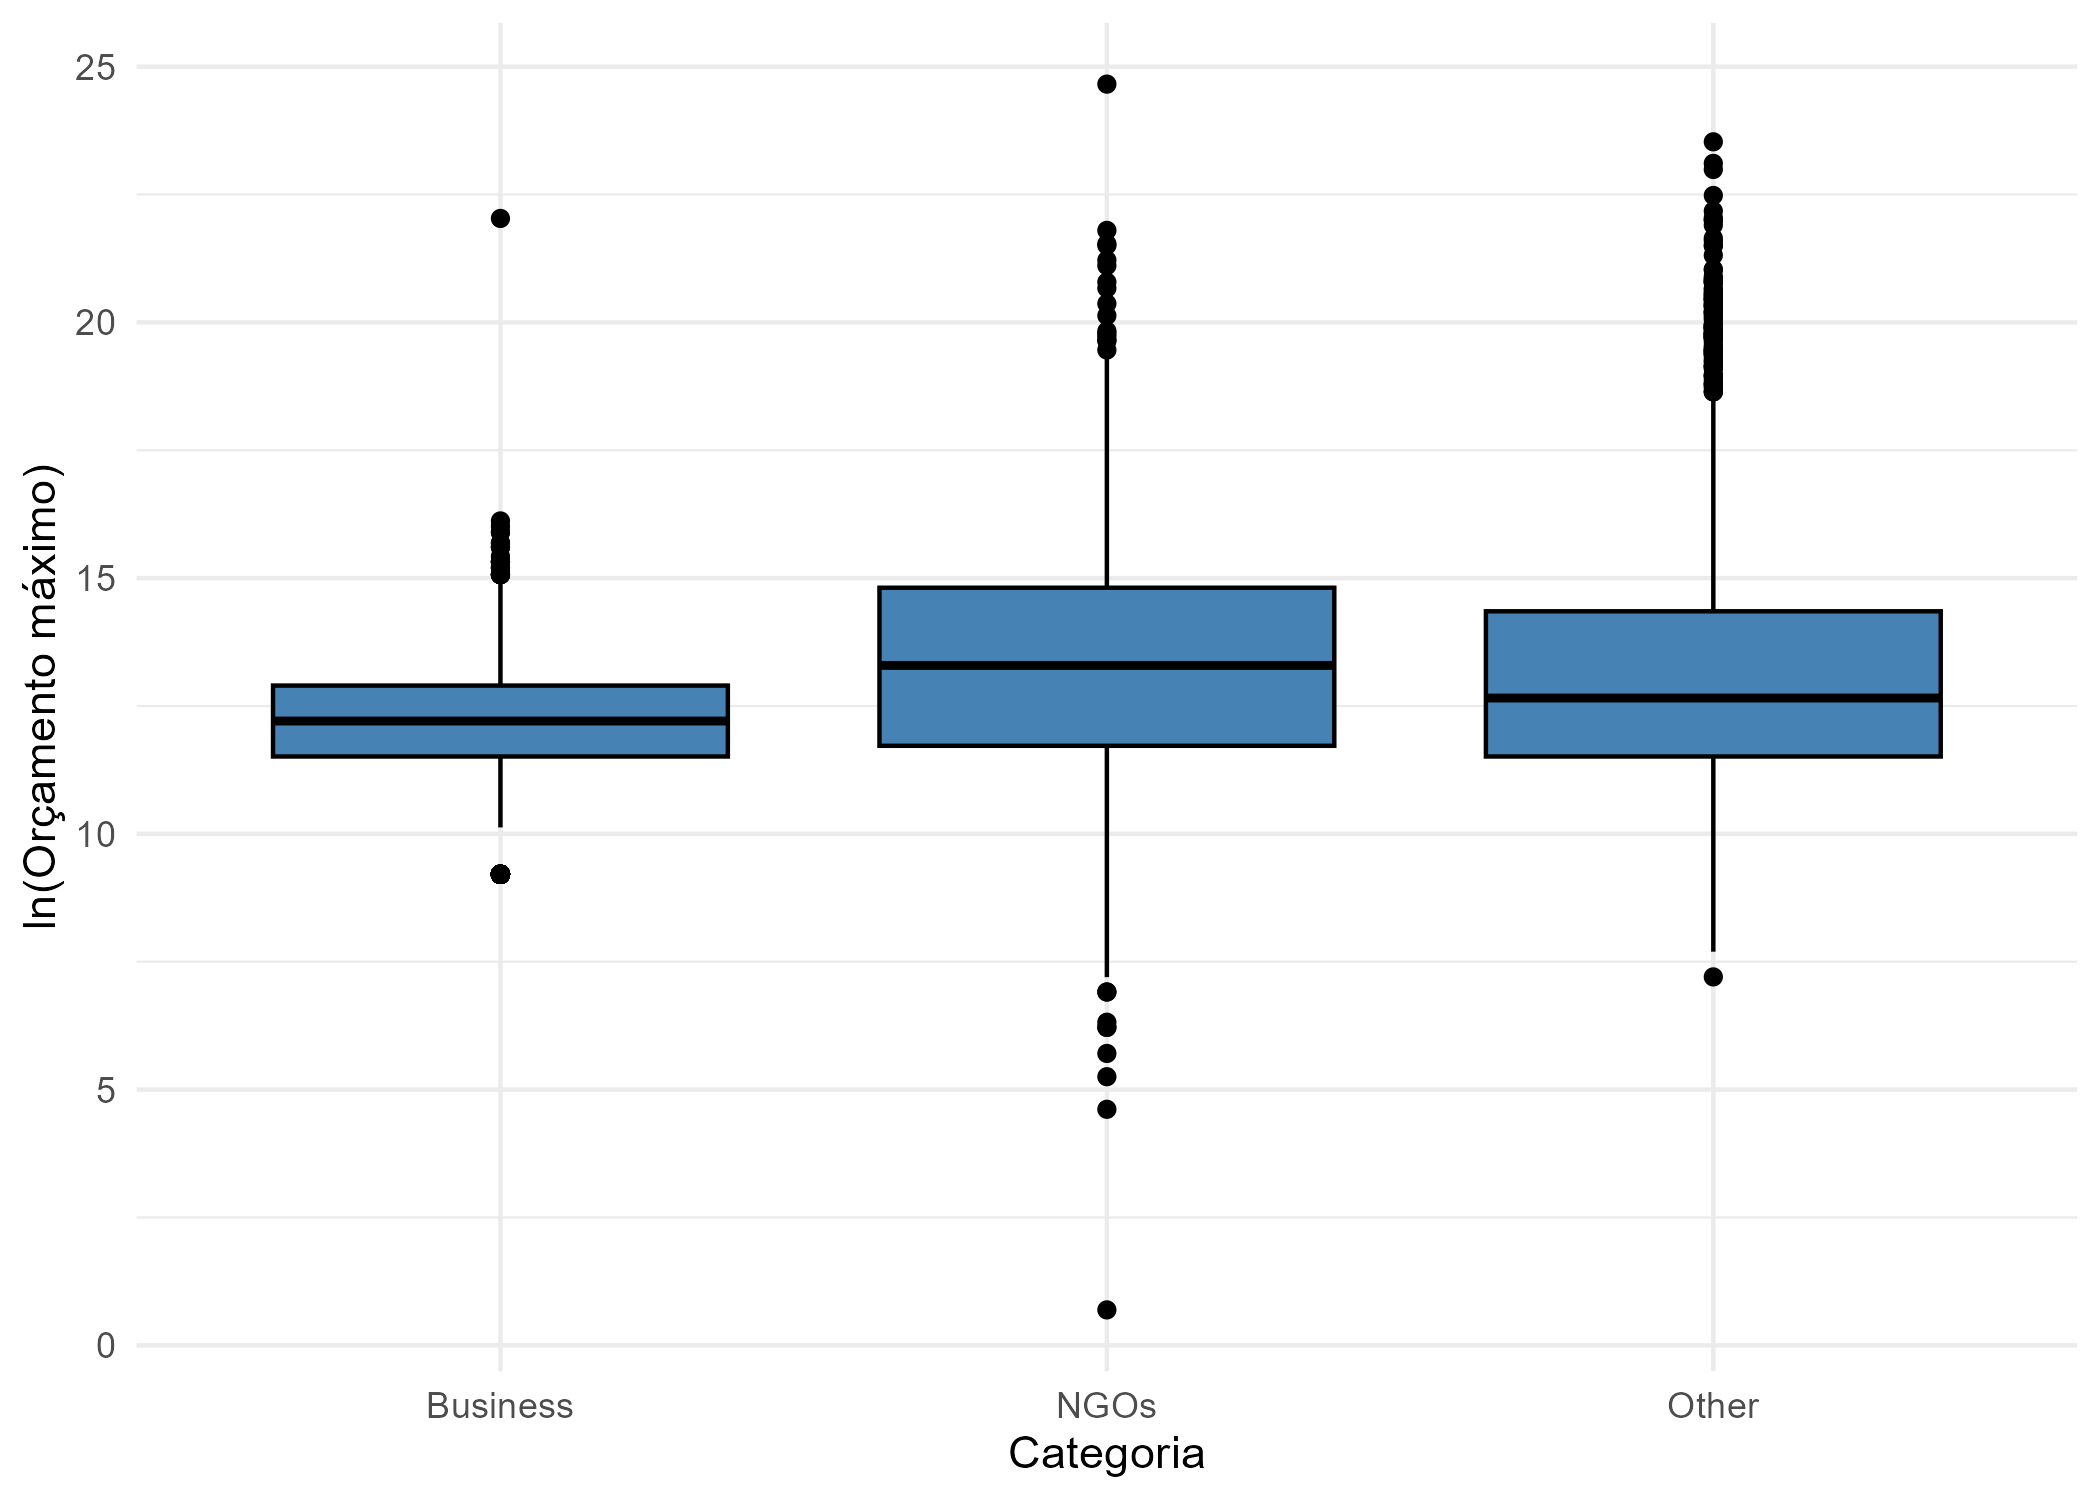
\includegraphics[width=0.75\textwidth]{figures/descriptives_lobbyists/boxplot_max_budget_by_category.png}
\caption{Distribuição de orçamento máximo declarado (\textit{ln(Orçamento Máximo Declarado)}) por categoria}
\label{fig:budget_ln_boxplot}
\end{figure}

Este achado é particularmente interessante, pois parece tensionar a premissa da literatura de que interesses empresariais dominam em termos de recursos financeiros \cite{de_figueiredo_advancing_2014, dur20212wholobbies}. Uma interpretação possível é que a categoria empresarial seja composta por um grande número de atores com gastos mais padronizados, enquanto as categorias de ONGs e "Outros" contêm algumas organizações muito grandes, cujos orçamentos massivos podem refletir campanhas de alto custo ou estruturas de financiamento distintas. A alta variância pode, ainda, ser um reflexo de diferentes estratégias: enquanto empresas podem ter um dispêndio mais constante, ONGs podem mobilizar grandes somas para temas de alta saliência, onde a opinião pública é um fator crucial \cite{mahoney_lobbying_2007}.

Adicionalmente, a concentração no grupo empresarial pode estar relacionada ao problema da ação coletiva \cite{olson1971logic}, onde muitas empresas optam por atuar por meio de associações — que podem estar classificadas na categoria "Outros". De todo modo, os dados reforçam que a relação entre recursos financeiros e influência não é direta \cite{simon_notes_1953}, e que a capacidade de mobilizar diferentes tipos de recursos — não apenas financeiros, mas também de legitimidade e informação \cite{Coen2019} — é central para a dinâmica do lobby na \acrshort{ue}.


% Distribuição geográfica
A análise da distribuição geográfica dos lobistas (Figura \ref{fig:country_distribution}) revela uma acentuada concentração em polos institucionais da União Europeia, com Bélgica (24,2\%), Alemanha (15,3\%) e França (10,1\%) abrigando a maioria das organizações. Este padrão corrobora a tese da vantagem da proximidade institucional: a presença massiva na Bélgica, sede da Comissão Europeia e de grande parte das atividades do Parlamento, e na França, que sedia as sessões plenárias do Parlamento em Estrasburgo, é uma resposta estratégica à complexa governança multinível da \acrshort{ue} \cite{richardson2000government}.

\begin{figure}[!htbp]
\centering
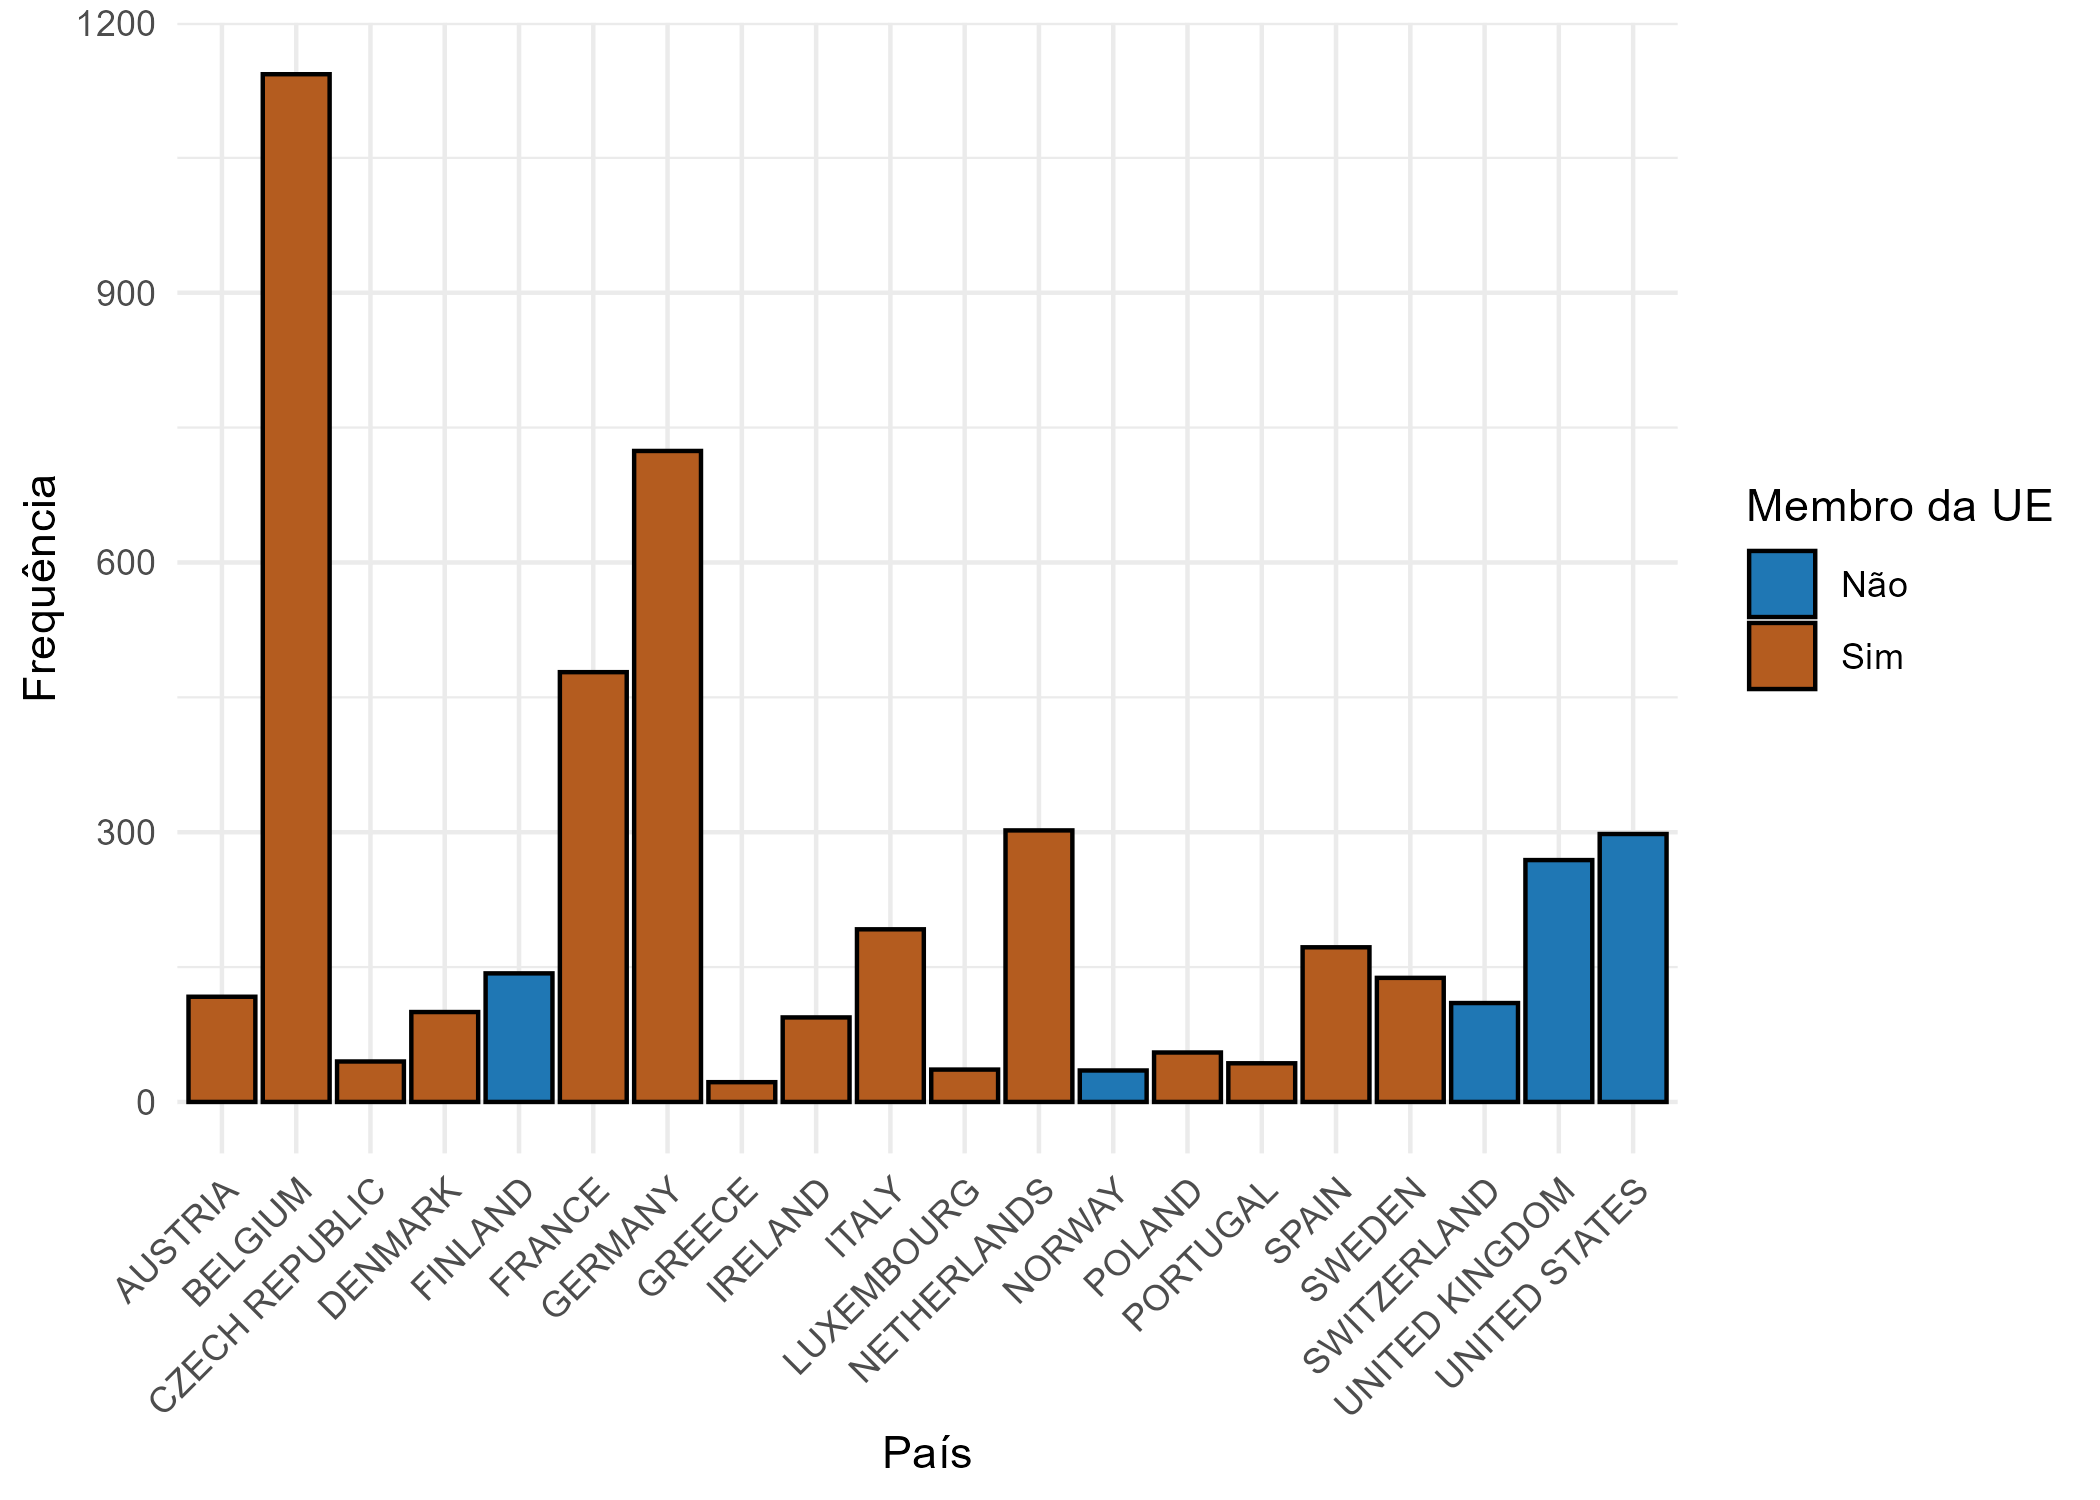
\includegraphics[width=0.9\textwidth]{figures/descriptives_lobbyists/barplot_country_distribution.png}
\caption{Top 20 países-sede (n = 4.516 organizações, totalizando 95,6\% do total de organizações)}
\label{fig:country_distribution}
\end{figure}

O fenômeno do \textit{venue-shopping} — a escolha estratégica do fórum mais favorável para exercer pressão — é central para entender essa distribuição \cite{kluver2015legislative}. A estrutura institucional da \acrshort{ue}, com poder decisório partilhado entre a Comissão, o Conselho e o Parlamento, incentiva os grupos de interesse a se estabelecerem nos locais onde podem monitorar e intervir mais eficazmente no ciclo político. A proeminência de países como Alemanha e França reflete não apenas a proximidade, mas também o peso político e econômico que exercem dentro da \acrshort{ue}.

Adicionalmente, a presença significativa de atores extracomunitários, que representam cerca de 20\% do total de organizações com sedes em 70 países (com destaque para os Estados Unidos, com 6,3\%), evidencia a importância da \acrshort{ue} como arena regulatória global. A atratividade do mercado europeu e o impacto de suas decisões incentivam atores internacionais a investir em uma presença local para influenciar a formulação de políticas que afetarão seus interesses. 

O recorte do top 20, que mostra uma cauda longa com muitos países de baixa frequência, reforça a ideia de que, embora o sistema seja permeável, os altos custos de manter uma operação de lobby eficaz na Europa centralizam a influência em atores com maiores recursos e localização estratégica.

% Distribuição temporal dos registros
Temporalmente, observa-se aceleração do registro de entidades após meados da década de 2010, com 2023 concentrando 17,9\% do total. Picos intermediários (2015--2016; 2020--2022) são compatíveis com ciclos legislativos, janelas regulatórias e alterações incrementais nos mecanismos de transparência.

\begin{figure}[!htbp]
\centering
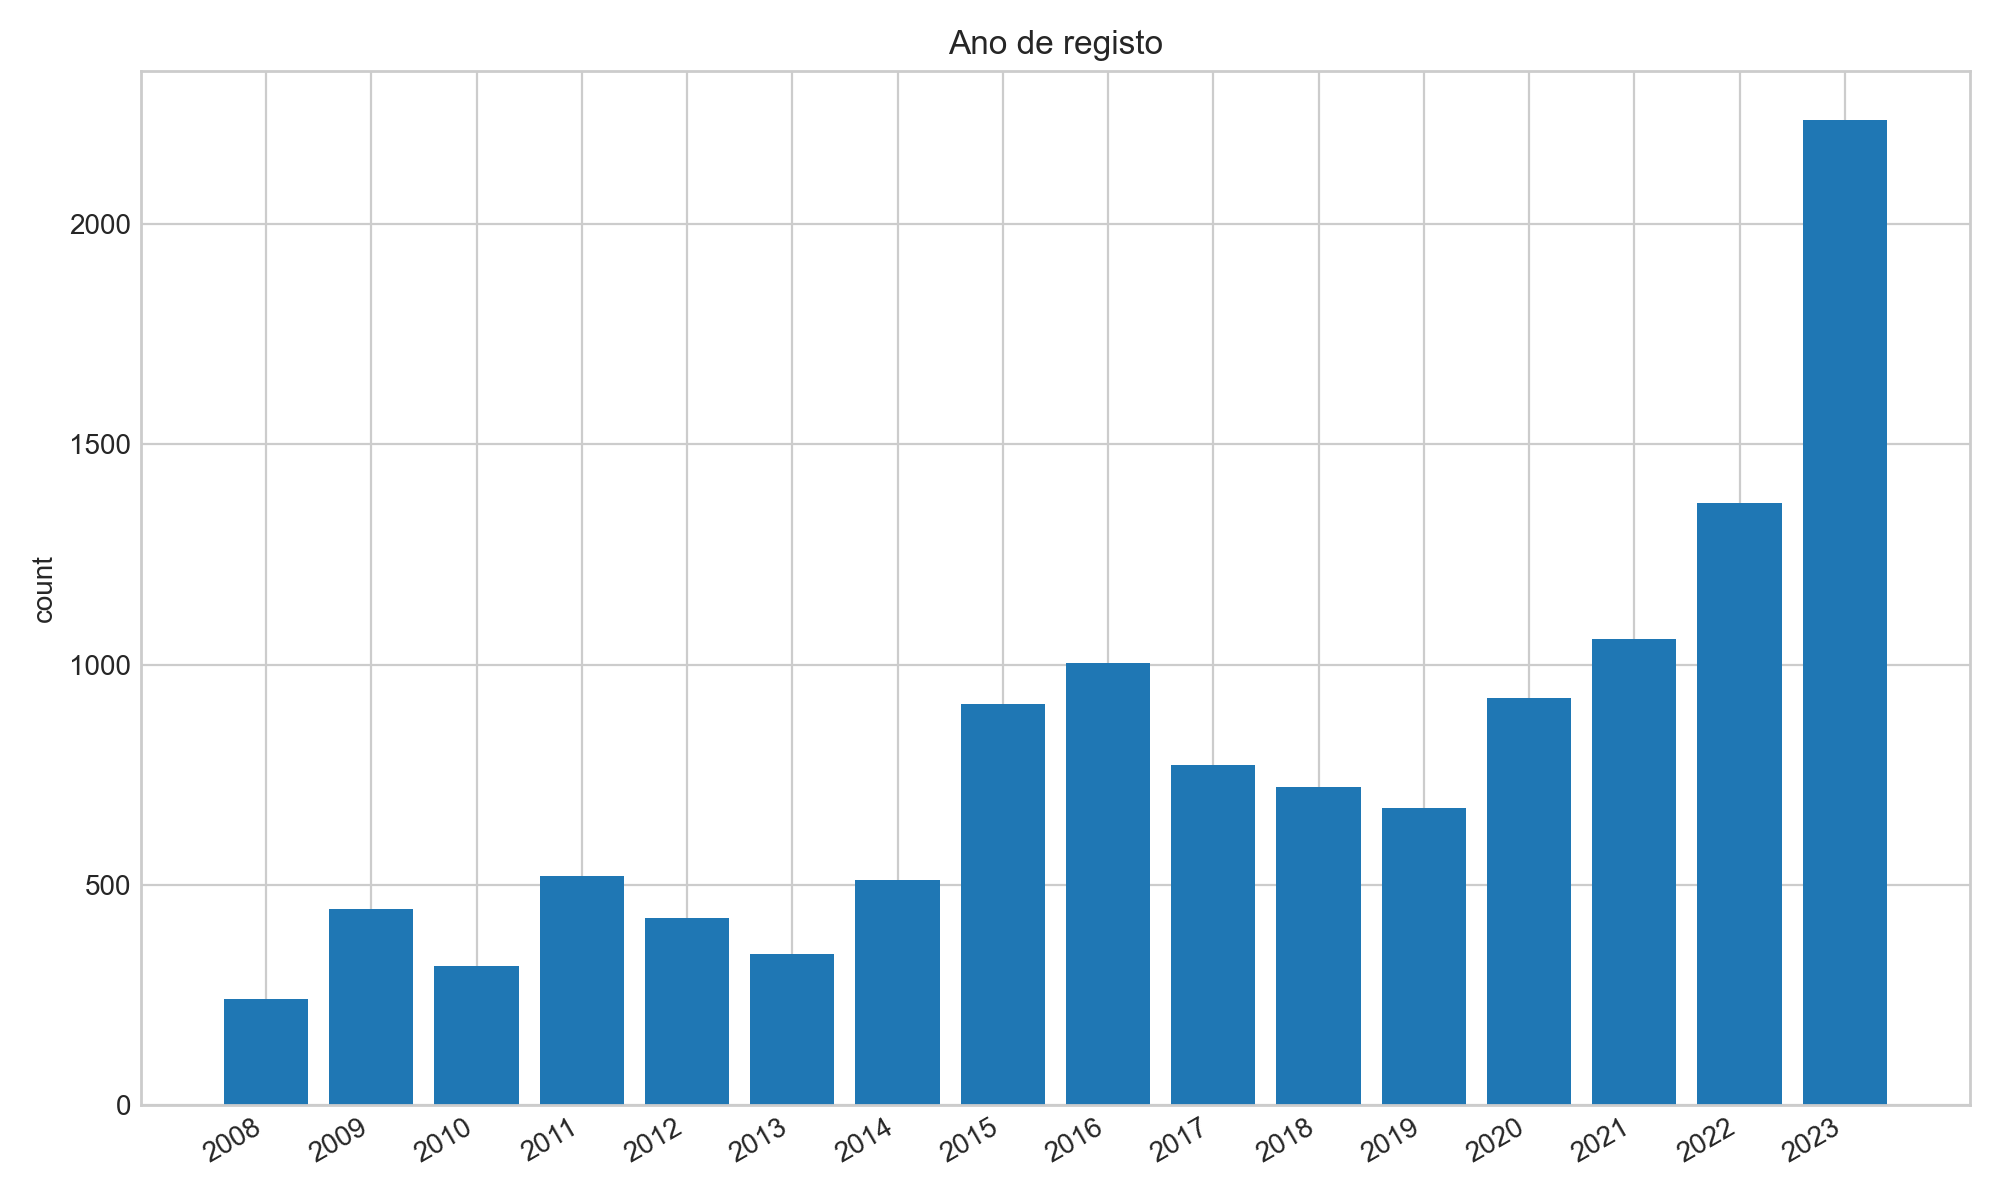
\includegraphics[width=0.75\textwidth]{figures/year_distribution.png}
\caption{Ano de registo}
\end{figure}

O padrão visual sugere crescimento estrutural recente do ecossistema de representação de interesses, possivelmente associado às agendas de transição digital e verde e à recomposição pós-pandemia.

% Distribuição temática
As incidências por domínio (Figura \ref{fig:theme_coverage}) destacam \textit{Economia e Comércio} (15\%), \textit{Tecnologia} (14,9\%) e \textit{Infraestrutura e Indústria} (14,4\%), seguidas por \textit{Tecnologia} (14,2\%) e \textit{Meio Ambiente e Clima} (13,8\%). Temas como \textit{Saúde} (9,8\%) e \textit{Educação} (8,1\%) são intermediários; \textit{Agricultura} (7,2\%) e \textit{Direitos Humanos} (6,2\%) têm menor incidência relativa.

\begin{figure}[!htbp]
\centering
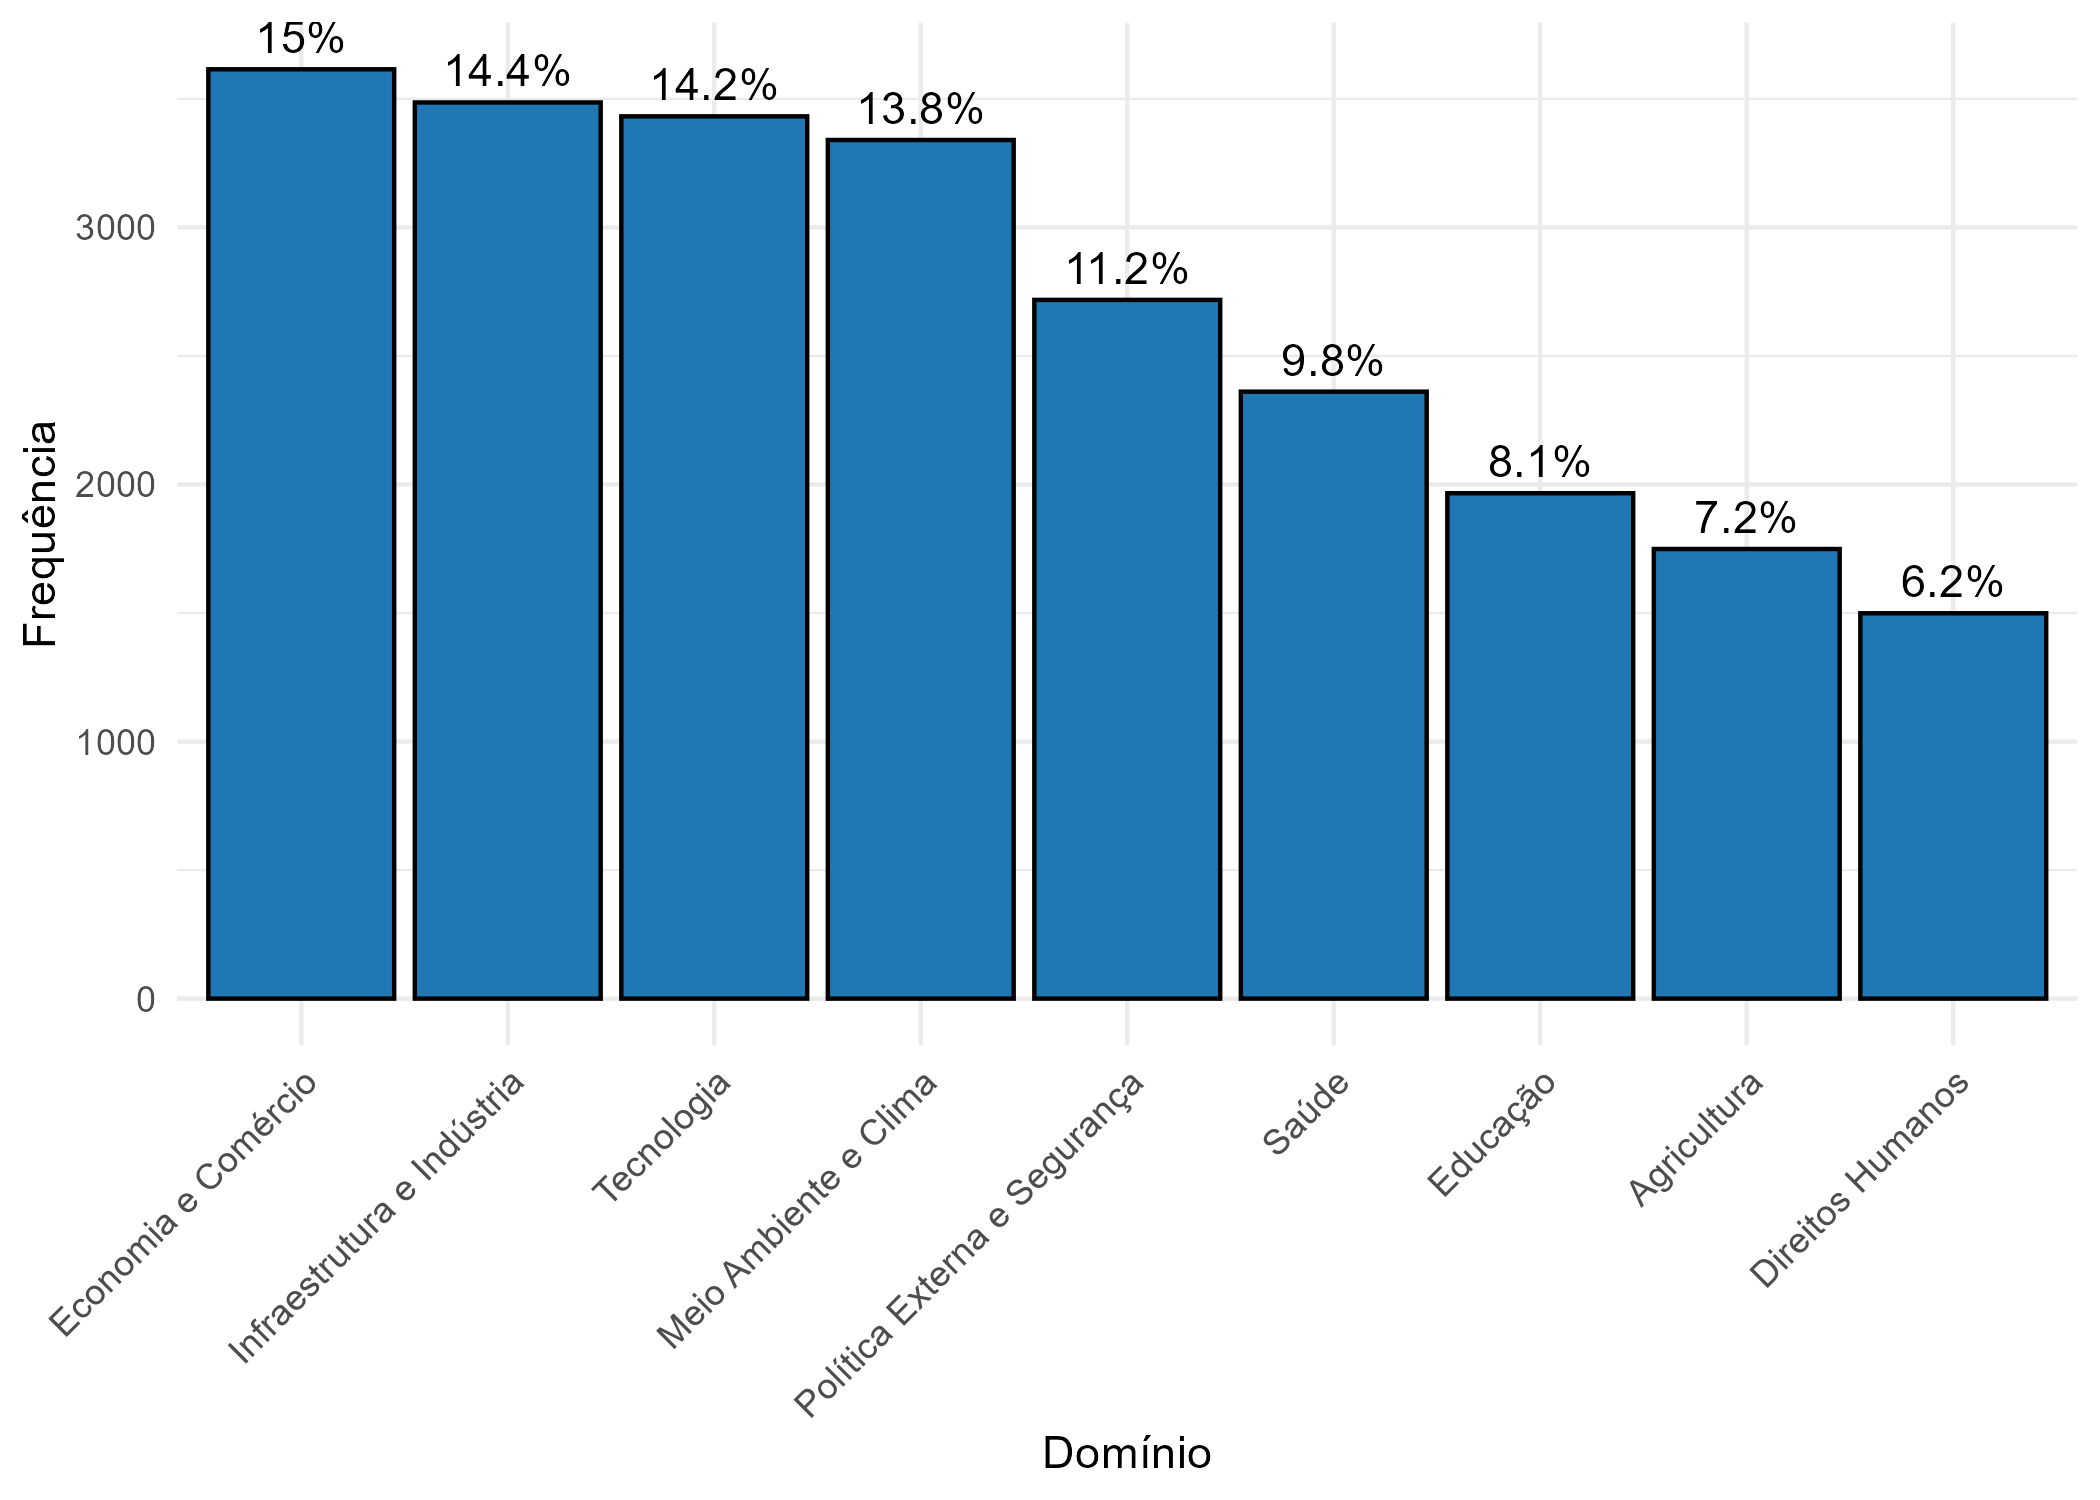
\includegraphics[width=0.9\textwidth]{figures/descriptives_lobbyists/barplot_domain_distribution.png}
\caption{Cobertura temática (proporção de entidades)}
\label{fig:theme_coverage}
\end{figure}

A distribuição temática (Figura \ref{fig:theme_coverage}) reflete uma concentração estratégica de esforços de lobby nas arenas de maior peso econômico e regulatório da União Europeia. A proeminência de domínios como "Economia e Comércio", "Infraestrutura e Indústria" e "Tecnologia" está alinhada com a literatura que demonstra uma correlação positiva entre a atividade de lobby e a saliência de um tema \cite{caldeira2000lobbying, baumgartner2010agendas}. São áreas onde as decisões políticas implicam altas consequências financeiras, mobilizando um volume expressivo de atores.

Adicionalmente, esses temas são caracterizados por uma elevada complexidade técnica. Este fator aumenta a demanda por informação especializada por parte dos decisores políticos, criando um vácuo que os lobistas buscam preencher para ganhar acesso e exercer influência, conforme sugere a literatura sobre o papel informacional do lobby \cite{kluver_informational_2012}. A própria agenda política da \acrshort{ue}, com iniciativas centrais como o Mercado Único Digital e o Pacto Ecológico Europeu, transforma esses domínios em focos de intensa atividade, corroborando a ideia de que os grupos de interesse são mais ativos nos temas em que o Estado também é mais atuante \cite{mahoney2008brussels}.

Em contraste, temas como "Direitos Humanos" e "Agricultura", embora relevantes, apresentam menor incidência relativa. Isso pode indicar que os interesses difusos ou setoriais dessas áreas enfrentam maiores desafios de ação coletiva ou utilizam estratégias de influência distintas, que não se refletem com a mesma intensidade no lobby direto. O padrão observado, portanto, sugere um ecossistema de lobby que responde de forma racional tanto aos incentivos econômicos quanto às necessidades informacionais geradas pela agenda regulatória da UE.

\begin{figure}[!htbp]
\centering
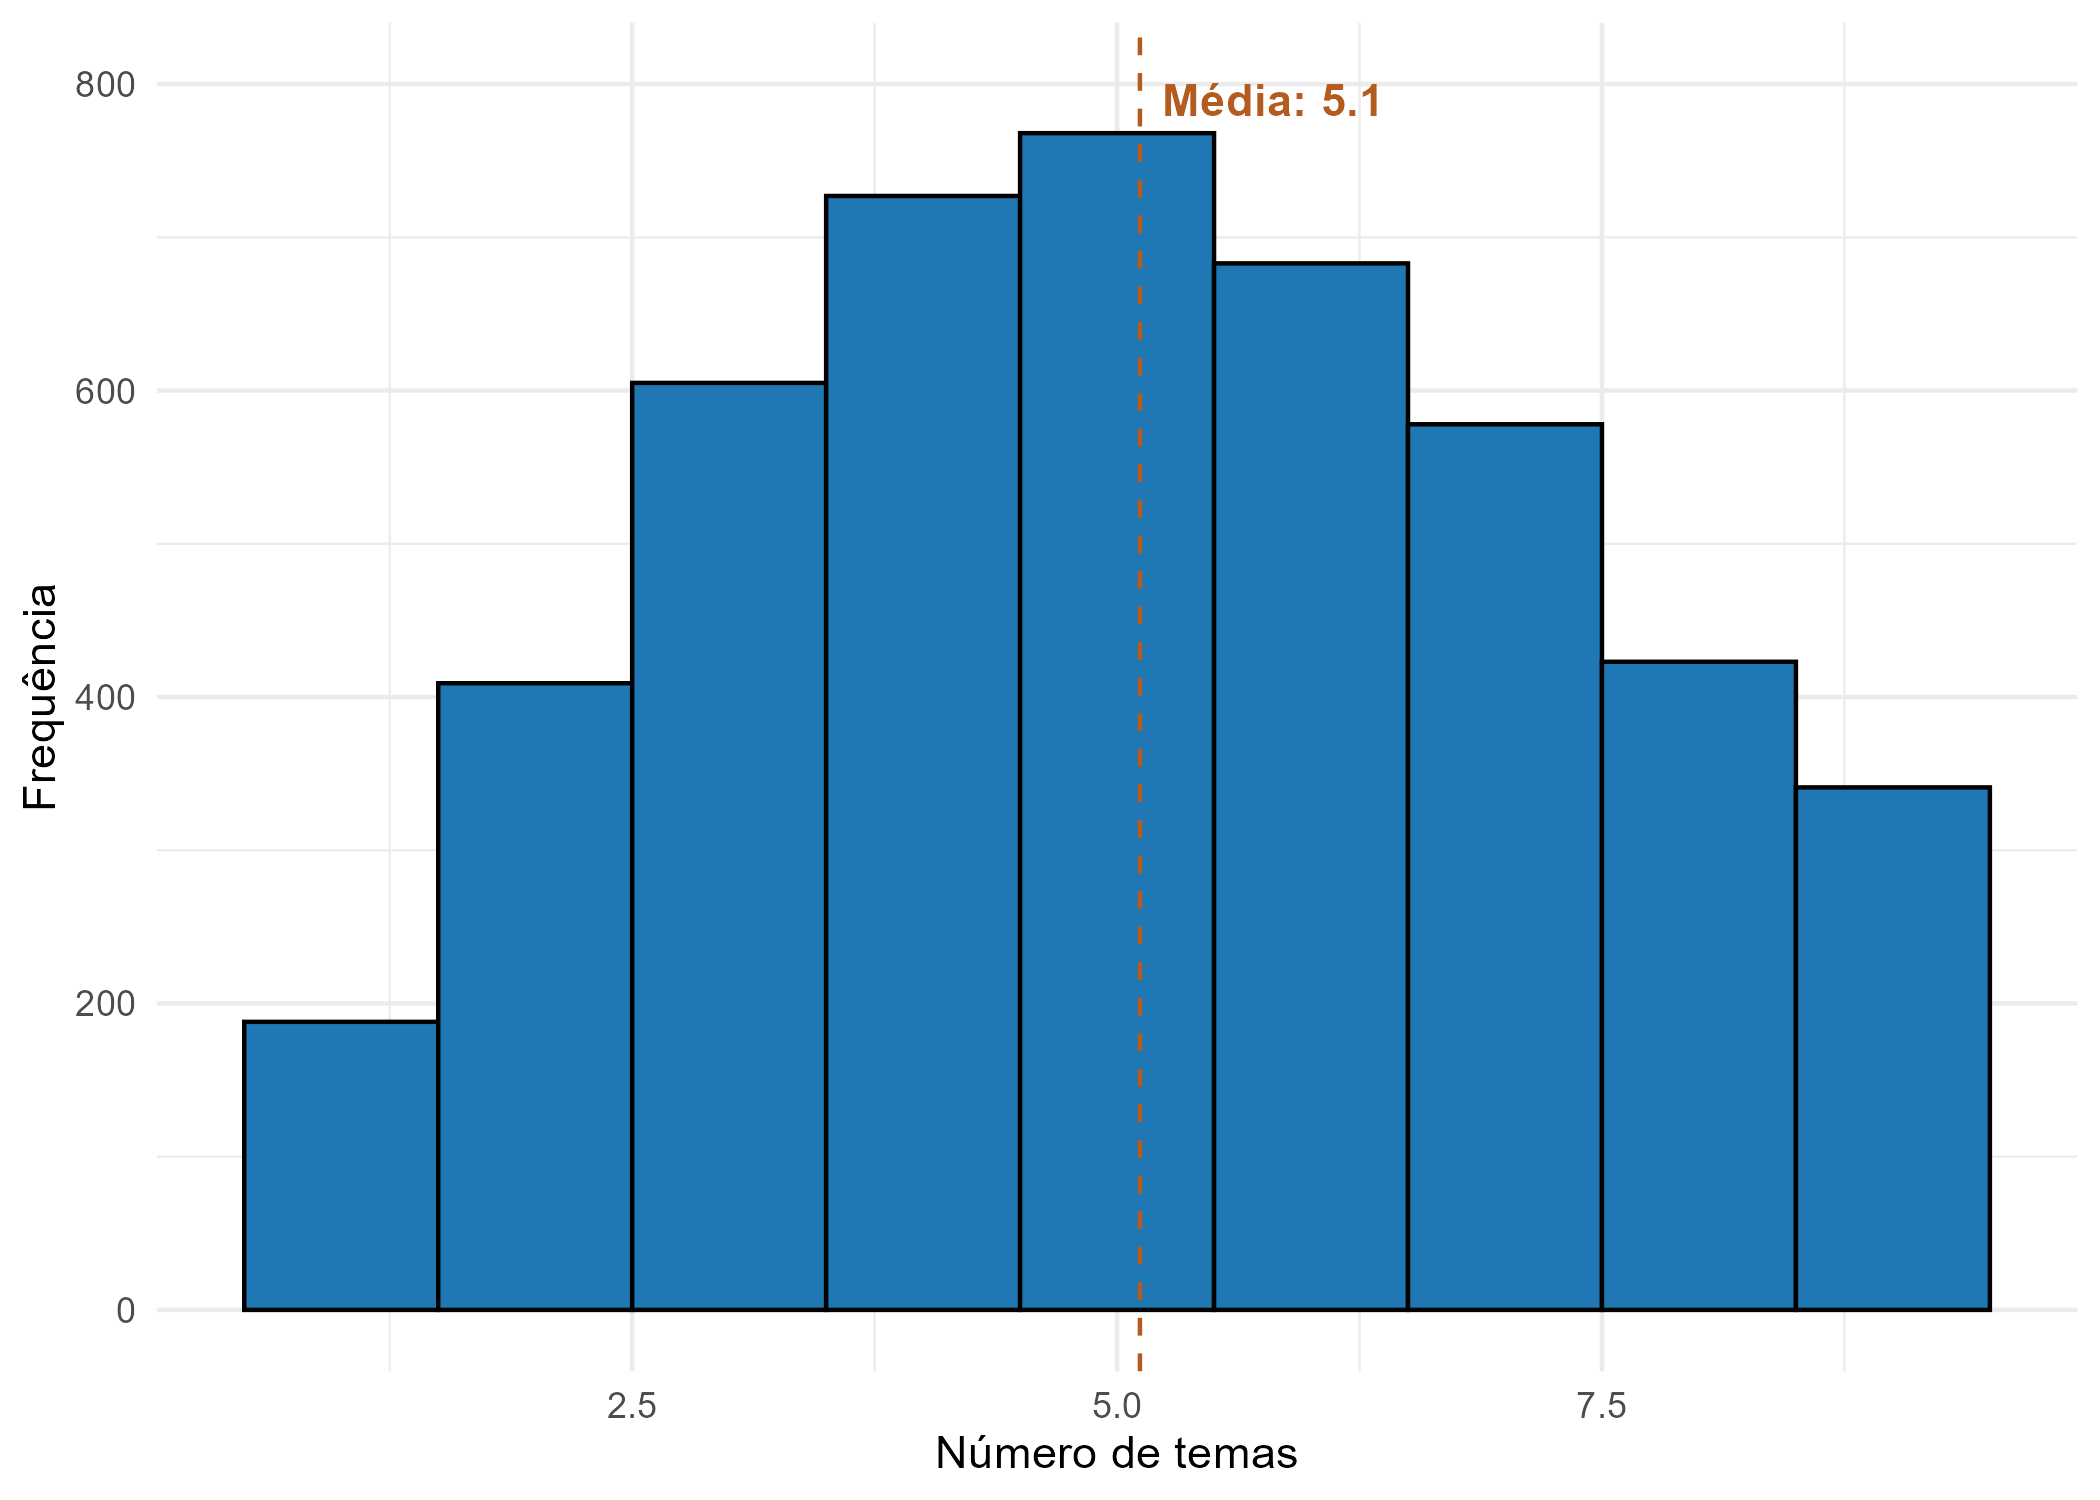
\includegraphics[width=0.75\textwidth]{figures/descriptives_lobbyists/histogram_themes_per_lobbyist.png}
\caption{Número de temas por lobista}
\label{fig:themes_per_lobbyist_hist}
\end{figure}

A análise da diversidade temática das organizações (Figura \ref{fig:themes_per_lobbyist_hist}) revela que a maioria dos lobistas atua em múltiplas frentes. A distribuição, que se assemelha a uma curva normal com média de 5,1 temas por organização, demonstra a coexistência de estratégias especializadas (focadas em poucos temas) e generalistas. Contudo, o padrão dominante é o de uma abordagem multi-temática, onde as organizações cobrem um portfólio de 3 a 7 áreas de interesse.

Este achado dialoga diretamente com o debate na literatura sobre os recursos mais valiosos para o lobby: expertise ("o que você sabe") versus conexões ("quem você conhece") \cite{bertrand2014whom}. A presença de atores especializados sugere uma aposta na expertise técnica como via de influência, especialmente em domínios de alta complexidade \cite{kluver_informational_2012}. Por outro lado, a predominância de atores multi-temáticos indica que uma estratégia mais ampla, possivelmente baseada em redes de contatos e na capacidade de adaptação a diferentes arenas políticas, é a norma no complexo ambiente institucional da \acrshort{ue}. A governança multinível e a interconexão de políticas na Europa podem incentivar as organizações a não se limitarem a um único nicho, buscando pontos de acesso em diferentes comissões e agências \cite{coen2019legislative}.

Em conjunto, os resultados descritivos apontam para um ecossistema plural, geograficamente ancorado em polos institucionais centrais, com dinamismo temporal recente e agendas orientadas por digitalização, competitividade industrial e sustentabilidade. Esses padrões informam as escolhas de especificação nos capítulos seguintes, notadamente a estratificação por perfis organizacionais, a construção de domínios temáticos e o controle para tendências temporais.


Os resultados descritivos delineiam um panorama abrangente do universo de lobistas registados junto às instituições europeias. Em primeiro lugar, a distribuição por categoria revela a coexistência de diferentes perfis organizacionais (\textit{Empresas}, \textit{\acrshort{ong}s} e \textit{Outros}), com magnitudes comparáveis entre atores empresariais e organizações da sociedade civil. Essa composição é compatível com a literatura sobre pluralismo organizacional e competição por acesso institucional no contexto da \acrshort{ue}, sugerindo um campo de ação onde interesses difusos e concentrados buscam simultaneamente agenda e influência.

Em síntese, as evidências descritivas apontam para um ecossistema plural, geograficamente ancorado em polos institucionais centrais, com dinamismo temporal recente e agendas orientadas por digitalização, competitividade industrial e sustentabilidade. Esses padrões informam as escolhas de especificação nos capítulos seguintes, notadamente a estratificação por perfis organizacionais, a construção de domínios temáticos e o controle para tendências temporais.


\section{Análise descritiva do tratamento}
\label{sec:resultados_descritica}

Esta seção apresenta uma análise descritiva sistemática dos dados utilizados para investigar os efeitos do lobbying na atividade parlamentar dos deputados do Parlamento Europeu. A abordagem adotada segue uma estratégia analítica multinível, iniciando com padrões agregados gerais e progredindo para análises desagregadas mais específicas. Esta progressão metodológica permite compreender tanto as tendências globais quanto os mecanismos específicos que operam no nível individual e temporal.

O conjunto de dados constitui um painel balanceado que combina informações sobre atividade parlamentar (perguntas) e intensidade de lobbying (reuniões) para 1.353 deputados ao longo de 63 meses, de julho de 2019 a novembro de 2024 em 9 domínios de política pública. Esta estrutura temporal permite capturar variações tanto na dimensão \textit{cross-sectional} (entre deputados e domínios) quanto longitudinal (evolução temporal), fornecendo a base empírica necessária para estratégias de identificação causal robustas.

Considerando a unidade de análise a tríade MEP-domínio-mês, temos 767.151 observações com taxa de completude de 100\%. Esta estrutura balanceada é metodologicamente vantajosa, pois elimina preocupações com viés de seleção decorrente de atrito amostral e garante que as estimativas não sejam distorcidas por padrões de observações ausentes.

A cobertura temporal de julho de 2019 a novembro de 2024 é particularmente relevante por abranger períodos de intensa atividade legislativa europeia, incluindo a transição entre legislaturas e eventos político-econômicos significativos. Destaca-se, nesse intervalo, o impacto da pandemia de COVID-19, que afetou profundamente tanto a dinâmica da atividade parlamentar quanto as estratégias de lobbying. A pandemia resultou em mudanças substanciais nos modos de trabalho do Parlamento Europeu, com a adoção de sessões remotas e restrições a reuniões presenciais, o que pode ter alterado padrões de interação entre deputados e grupos de interesse. Assim, a análise cobre não apenas períodos de normalidade institucional, mas também um contexto de crise sanitária global, permitindo investigar como choques exógenos desse tipo influenciam o comportamento político e o lobbying.

A \autoref{fig:time_series} apresenta a evolução temporal das variáveis principais no nível mais agregado, revelando padrões que são fundamentais para compreender a dinâmica do sistema político europeu ao longo do período estudado.

\begin{figure}[htbp]
\centering
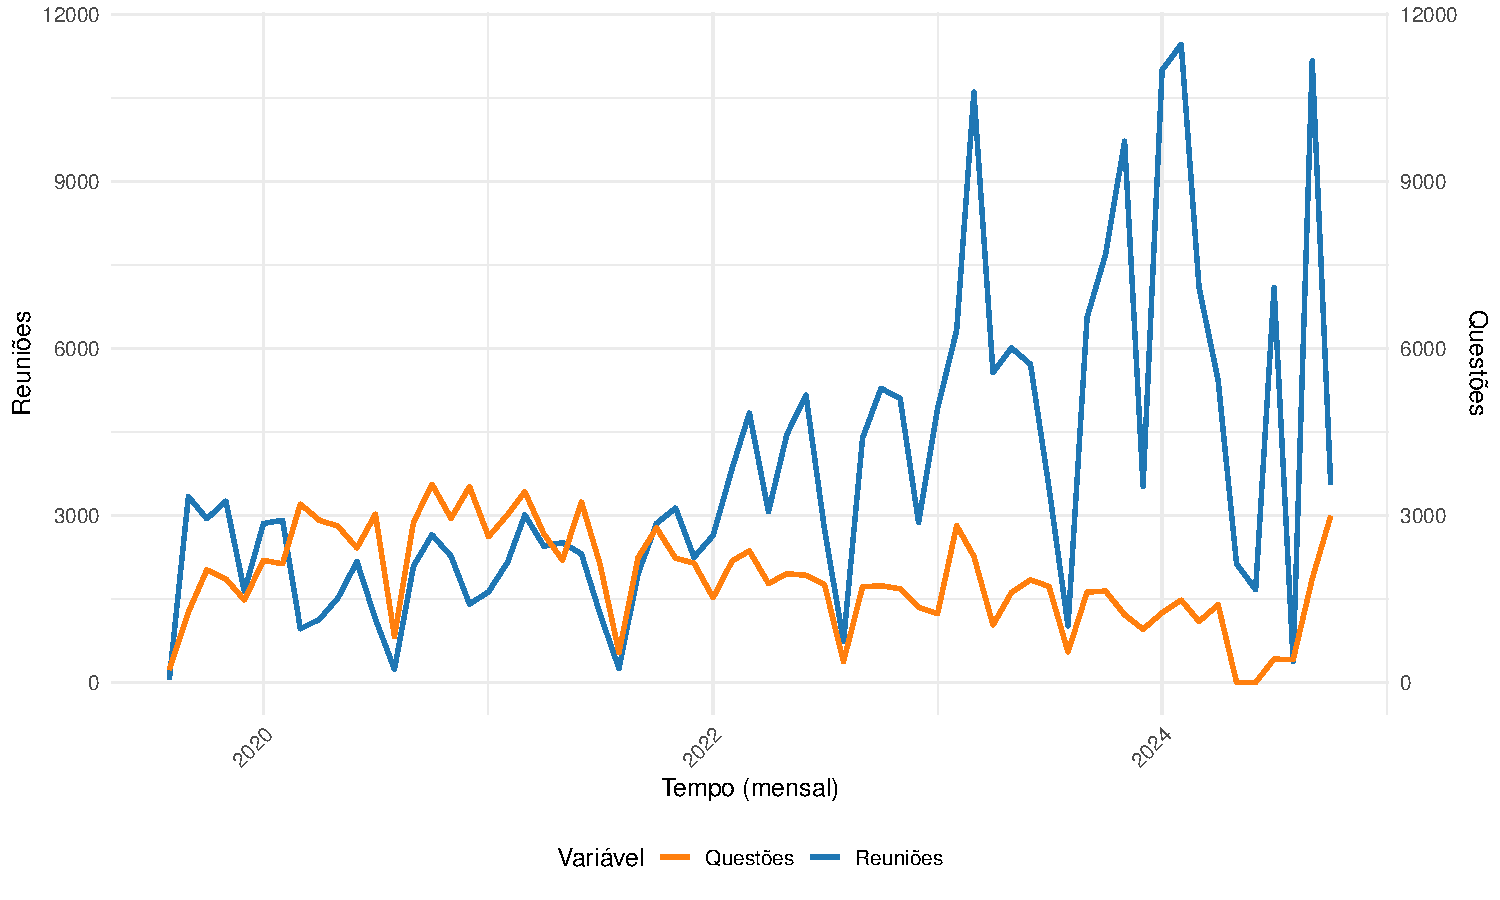
\includegraphics[width=\textwidth]{figures/fig1_time_series_meetings_questions.pdf}
\caption{Evolução temporal da atividade parlamentar e de lobbying}
\label{fig:time_series}
% \note{O painel superior esquerdo mostra os totais mensais agregados de perguntas e reuniões. O painel superior direito apresenta as médias mensais por observação MEP-domínio. O painel inferior esquerdo mostra a evolução da proporção de observações com atividade de lobbying. O painel inferior direito apresenta a estabilidade da correlação contemporânea entre as variáveis ao longo do tempo.}
\end{figure}

A análise temporal revela quatro padrões empiricamente relevantes. Primeiro, observa-se uma \textbf{tendência crescente} em ambas as variáveis ao longo do período, sugerindo intensificação tanto da atividade parlamentar quanto do lobbying. Segundo, existe clara \textbf{sazonalidade} relacionada ao calendário parlamentar, com reduções sistemáticas durante períodos de recesso. Terceiro, identificam-se \textbf{picos de atividade} que coincidem com discussões de legislação relevante em domínios específicos, indicando resposta coordenada do sistema político. Quarto, a \textbf{correlação contemporânea} entre perguntas e reuniões permanece relativamente estável ao longo do tempo, sugerindo estabilidade estrutural na relação entre as variáveis.

% não há exatamente essa tendência cerescente...


Estes padrões temporais têm implicações metodológicas importantes. A presença de tendências temporais justifica a inclusão de efeitos fixos de tempo nas especificações econométricas para controlar choques temporais comuns. A sazonalidade observada valida a escolha da frequência mensal como unidade temporal, capturando variações de curto prazo sem introduzir ruído excessivo. A estabilidade da correlação fornece evidência preliminar contra quebras estruturais que poderiam comprometer a validade das estimativas.

% \subsection{Padrões de participação: análise agregada por deputado}

Complementando a análise temporal, é fundamental examinar os padrões de participação no nível individual dos deputados. Esta perspectiva agregada revela a distribuição da atividade de lobbying entre os parlamentares e fornece insights sobre a concentração e heterogeneidade dos fenômenos estudados.



As \autoref{fig:proportion_meetings}, \autoref{fig:correlation_meetings_questions} e \autoref{fig:meetings_hist} apresentam uma análise dos padrões de participação agregados por deputado, revelando aspectos da distribuição da atividade de lobbying no Parlamento Europeu que impactam a identificação causal.

% \begin{figure}[htbp]
% \centering
% 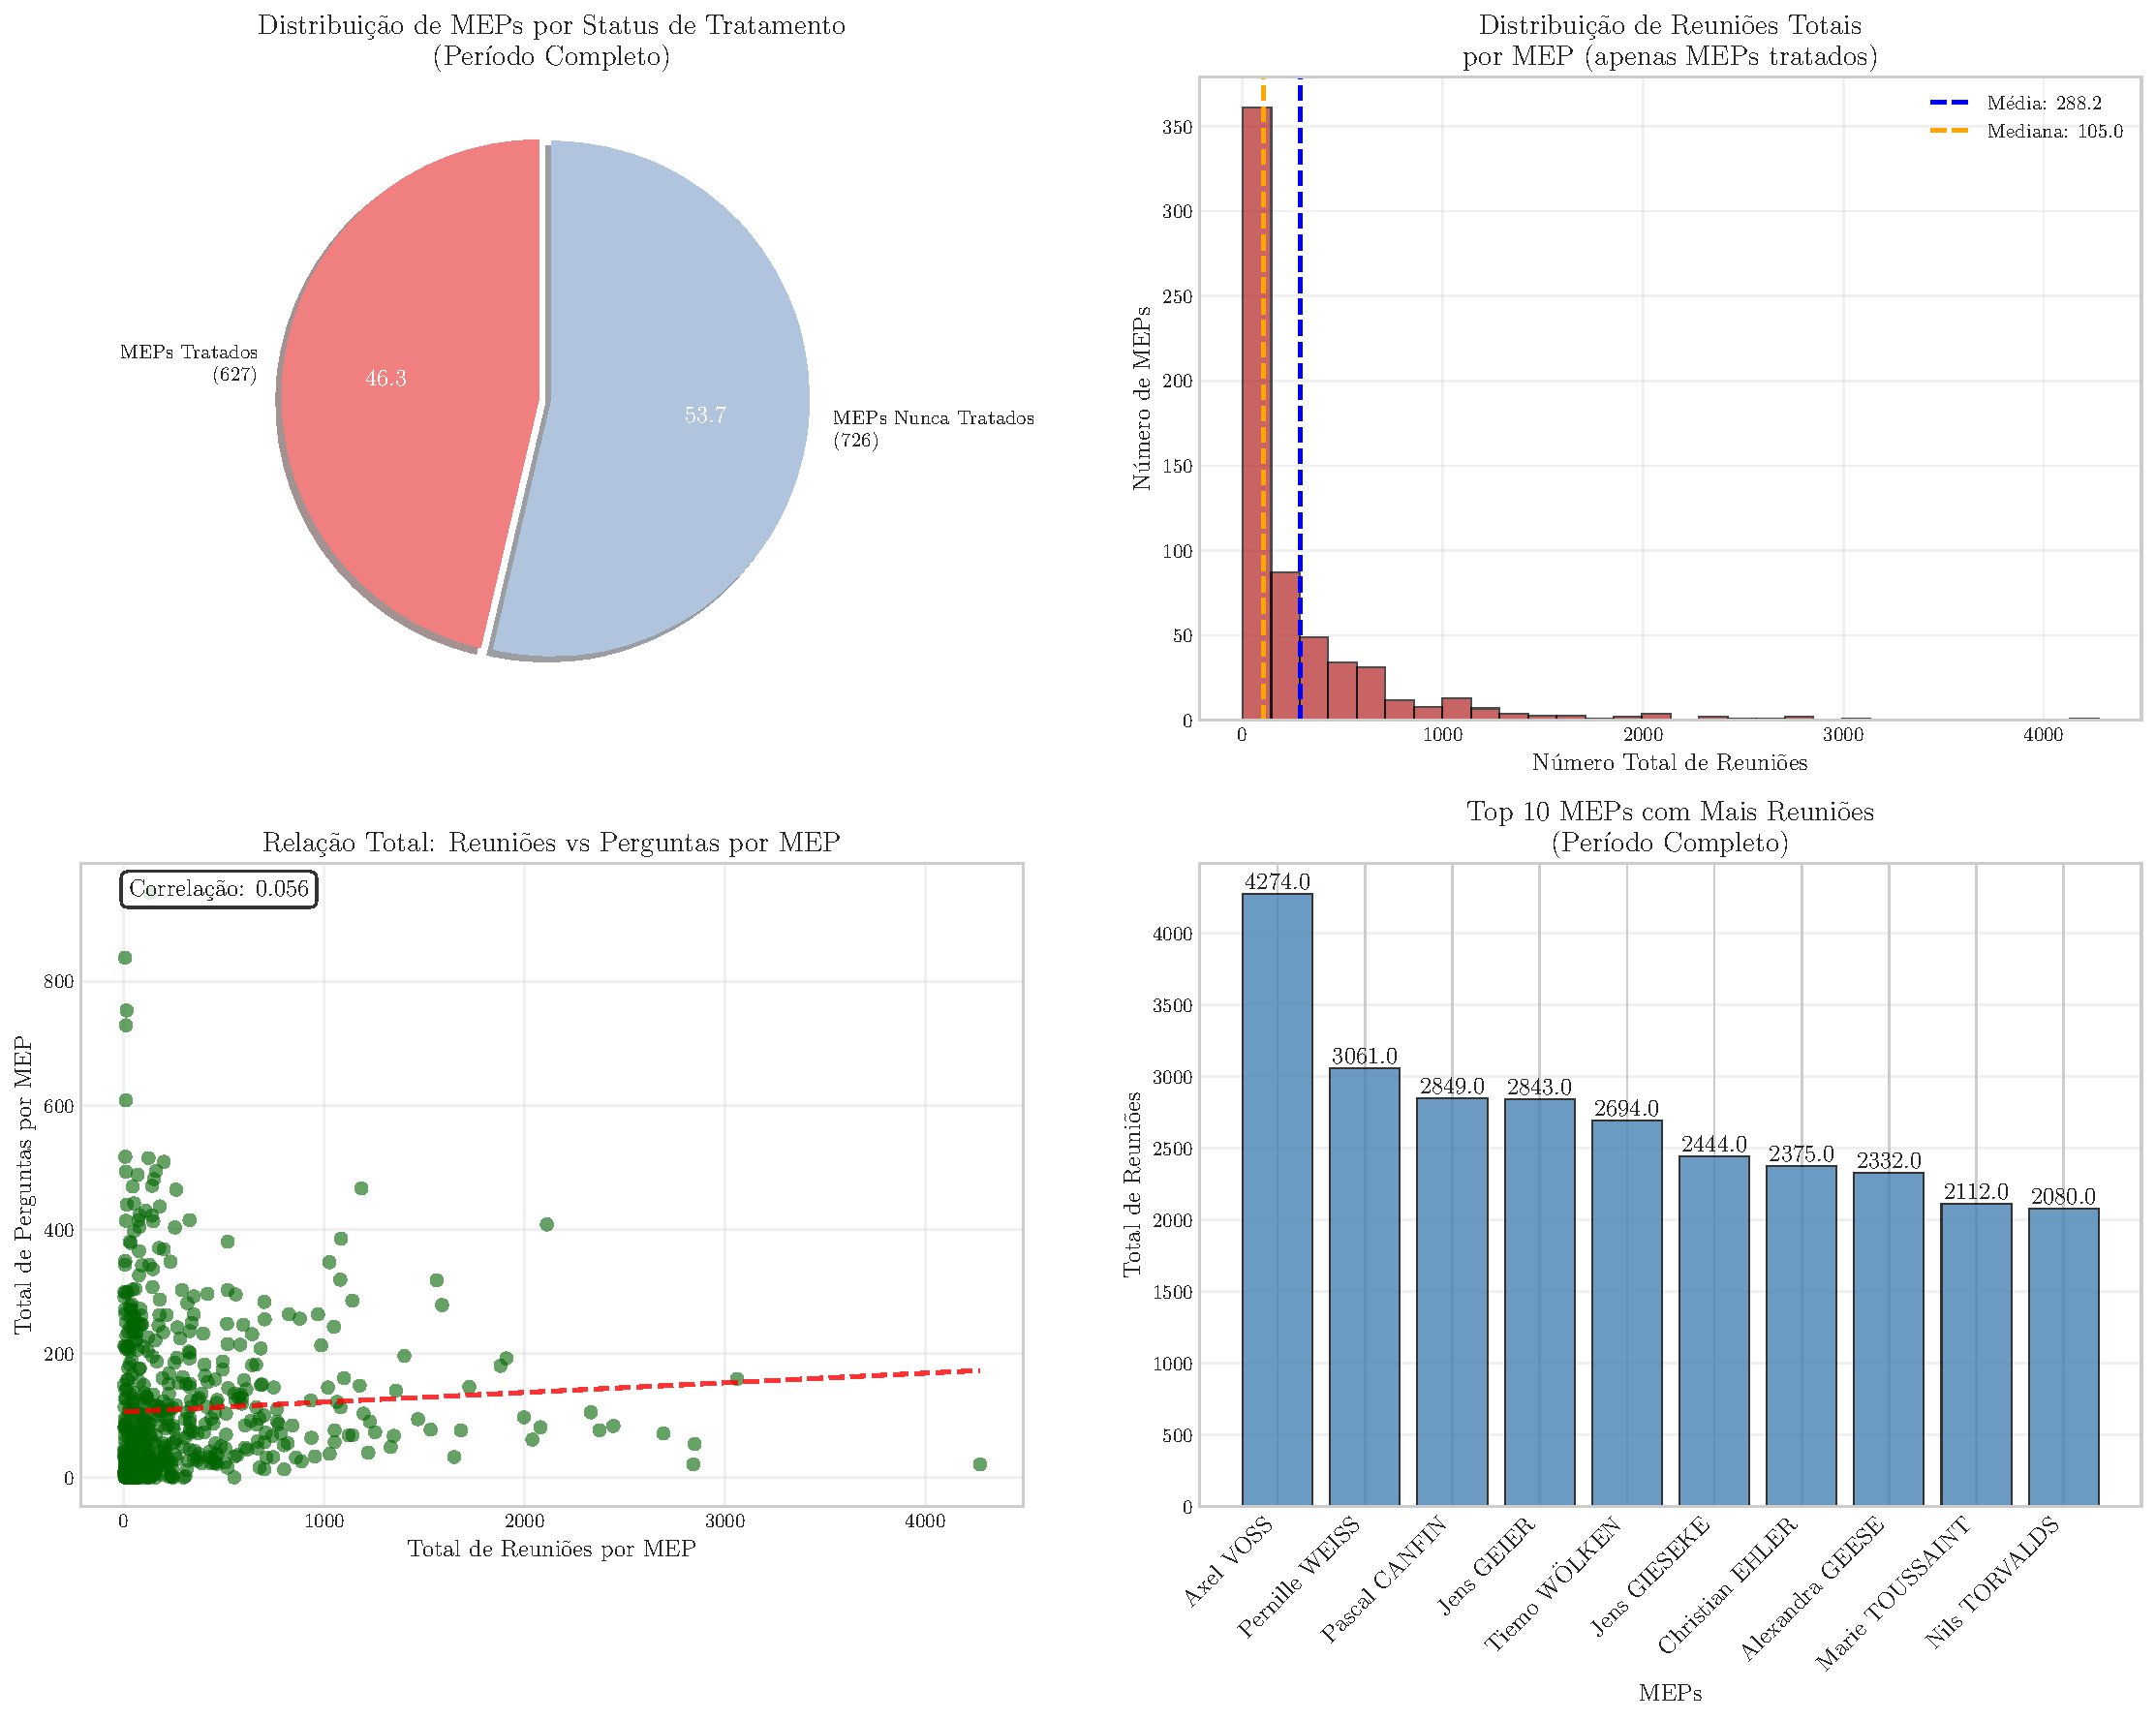
\includegraphics[width=\textwidth]{figures/fig6_mep_aggregated_analysis.pdf}
% \caption{Análise agregada por MEP: distribuição e intensidade do tratamento}
% \label{fig:mep_aggregated}
% \note{O painel superior esquerdo mostra a proporção de deputados que receberam pelo menos uma reunião de lobbying durante todo o período. O painel superior direito apresenta a distribuição da intensidade total de reuniões entre deputados tratados. O painel inferior esquerdo examina a relação agregada entre reuniões e perguntas totais por deputado. O painel inferior direito identifica os deputados mais ativos em termos de recepção de lobbying.}
% \end{figure}



% \subsubsection{Distribuição do tratamento entre deputados}

\begin{figure}[htbp]
    \centering
    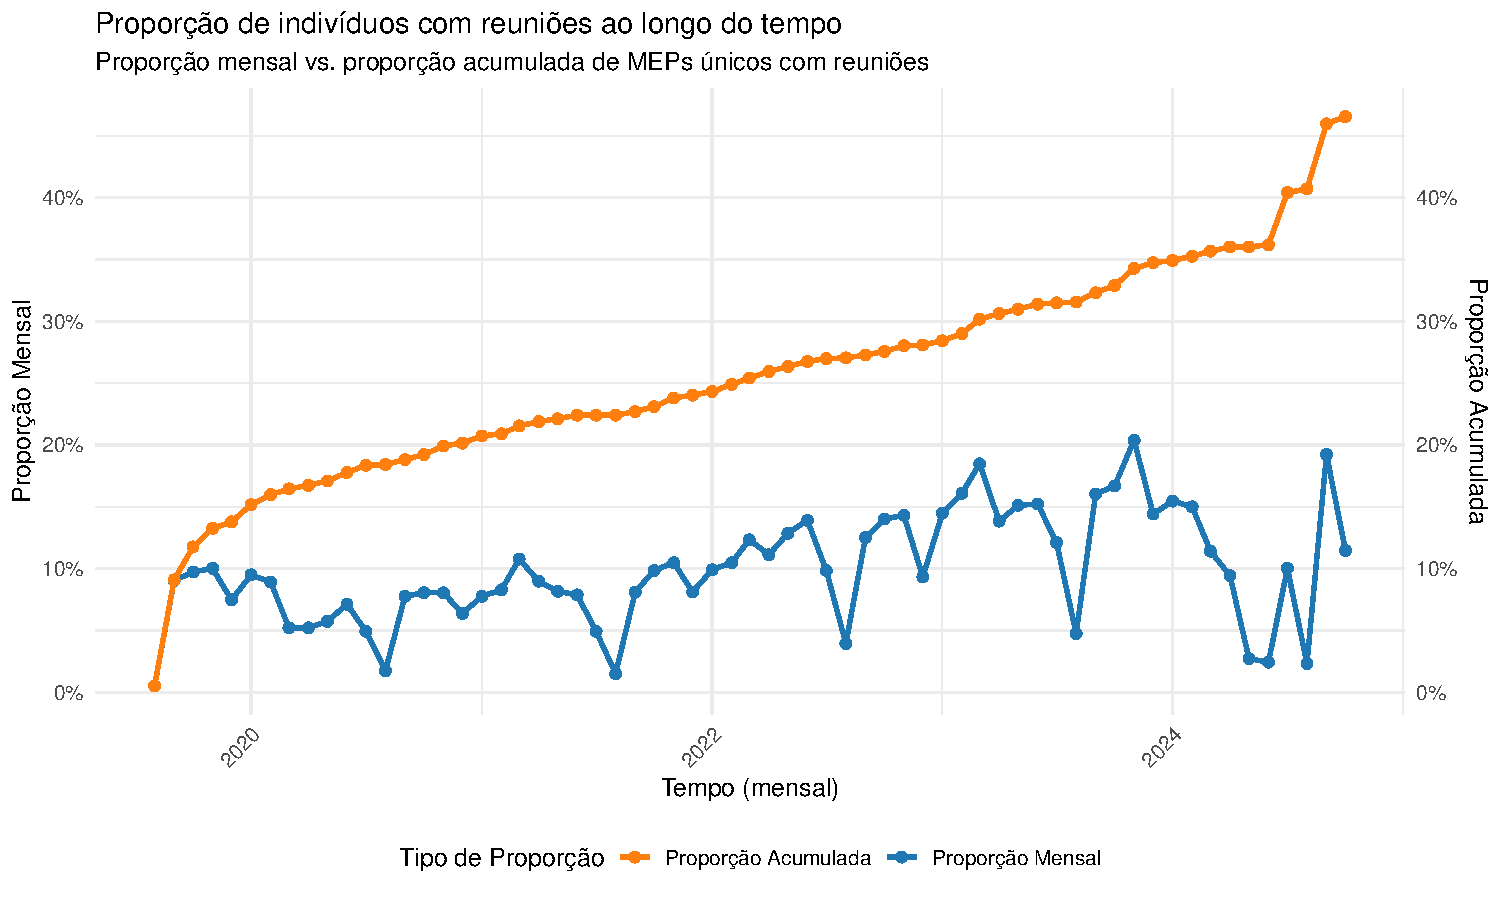
\includegraphics[width=\textwidth]{figures/fig2_proportion_meetings.pdf}
    \caption{Evolução temporal da proporção de \acrshort{mpe}s que participaram de reuniões de lobbying}
    \label{fig:proportion_meetings}
    % \note{O painel superior esquerdo mostra os totais mensais agregados de perguntas e reuniões. O painel superior direito apresenta as médias mensais por observação MEP-domínio. O painel inferior esquerdo mostra a evolução da proporção de observações com atividade de lobbying. O painel inferior direito apresenta a estabilidade da correlação contemporânea entre as variáveis ao longo do tempo.}
\end{figure}

\begin{figure}[htbp]
    \centering
    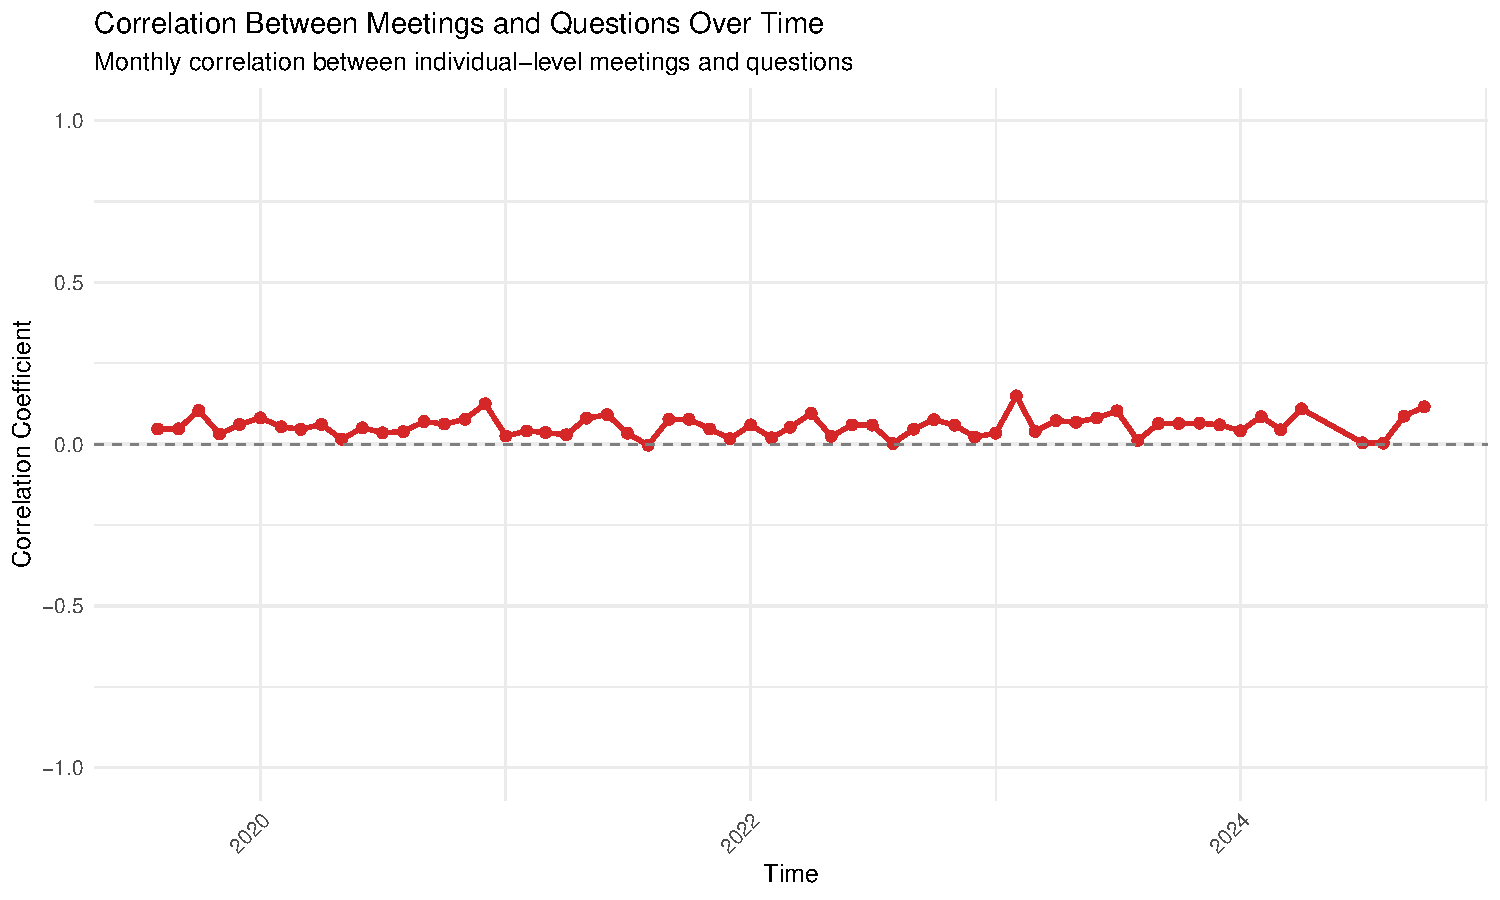
\includegraphics[width=\textwidth]{figures/fig3_correlation_meetings_questions.pdf}
    \caption{Evolução temporal da correlação entre reuniões e perguntas}
    \label{fig:correlation_meetings_questions}
    % \note{O painel superior esquerdo mostra os totais mensais agregados de perguntas e reuniões. O painel superior direito apresenta as médias mensais por observação MEP-domínio. O painel inferior esquerdo mostra a evolução da proporção de observações com atividade de lobbying. O painel inferior direito apresenta a estabilidade da correlação contemporânea entre as variáveis ao longo do tempo.}
\end{figure}

\begin{figure}[htbp]
    \centering
    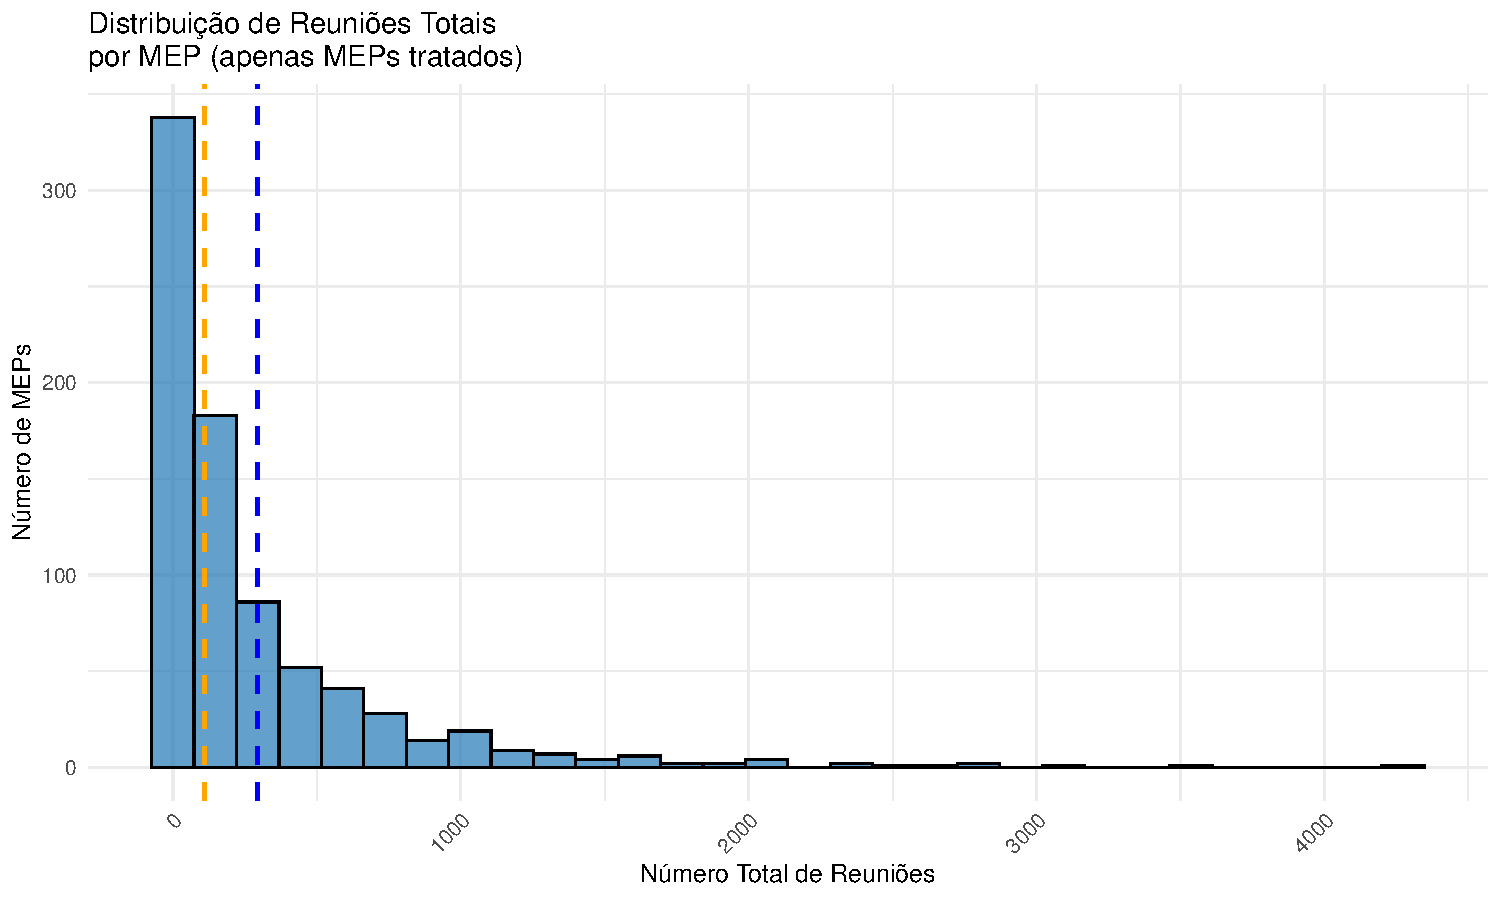
\includegraphics[width=\textwidth]{figures/fig3.1_meetings_hist.pdf}
    \caption{Distribuição de reuniões por \acrshort{mpe}}
    \label{fig:meetings_hist}
    % \note{O painel superior esquerdo mostra os totais mensais agregados de perguntas e reuniões. O painel superior direito apresenta as médias mensais por observação MEP-domínio. O painel inferior esquerdo mostra a evolução da proporção de observações com atividade de lobbying. O painel inferior direito apresenta a estabilidade da correlação contemporânea entre as variáveis ao longo do tempo.}
\end{figure}


A análise revela três características fundamentais da distribuição de tratamento. Primeiro, existe \textbf{participação substancial mas não universal}: 46,3\% dos deputados (637 de 1.353) receberam pelo menos uma reunião de lobbying durante o período estudado. Esta proporção indica que o lobbying é um fenômeno disseminado mas não ubíquo no sistema parlamentar europeu.

Segundo, observa-se \textbf{concentração extrema} na intensidade de tratamento. Entre os deputados que receberam lobbying, a distribuição é altamente assimétrica: enquanto a mediana é de 105 reuniões por deputado, a média é de 288,2 reuniões, indicando que uma minoria de parlamentares concentra uma proporção desproporcional da atividade lobista. O caso extremo de um deputado com 4.274 reuniões ilustra esta concentração.

Terceiro, a \textbf{correlação agregada} entre reuniões e perguntas totais por deputado é surpreendentemente baixa (0,056), contrastando com correlações mais elevadas observadas no nível temporal. Este padrão sugere que os efeitos do lobbying podem ser mais evidentes em frequências temporais específicas do que em padrões de atividade agregados de longo prazo.

% \paragraph{Implicações para a estratégia empírica}

Estes padrões agregados têm implicações importantes para a identificação causal. A concentração do tratamento em uma minoria de deputados sugere que estratégias de identificação baseadas em variação cross-sectional podem sofrer de poder estatístico limitado. Simultaneamente, a variação substancial na intensidade de tratamento entre deputados tratados fornece fonte valiosa de identificação para estimativas de dose-resposta.

A baixa correlação agregada, combinada com correlações temporais mais elevadas, indica que a identificação causal pode beneficiar-se de estratégias que explorem variação temporal within-individual rather than cross-sectional between-individual. Esta evidência preliminar orienta a especificação de modelos com efeitos fixos de deputado para controlar heterogeneidade não observada time-invariant.

\begin{table}[htbp]
\centering
\caption{Estatísticas agregadas de tratamento por deputado}
\label{tab:mep_treatment_stats}
\begin{tabular}{lr}
\toprule
\textbf{Estatística} & \textbf{Valor} \\
\midrule
Total de deputados únicos & 1{,}353 \\
Deputados que receberam tratamento & 627 \\
Taxa de tratamento por deputado (\%) & 46{,}3\% \\
\midrule
\textbf{Entre deputados tratados:} & \\
Reuniões médias por deputado & 288{,}2 \\
Reuniões medianas por deputado & 105{,}0 \\
Desvio padrão & 468{,}9 \\
Deputado mais ativo (reuniões) & 4{,}274 \\
\midrule
\textbf{Correlação agregada:} & \\
Correlação reuniões-perguntas & 0{,}056 \\
\bottomrule
\end{tabular}
\end{table}

\subsection{Heterogeneidade entre domínios de política pública}

A terceira dimensão da análise agregada examina a variação entre domínios de política pública. Esta heterogeneidade setorial é teoricamente relevante porque diferentes áreas de política podem apresentar características distintas em termos de complexidade técnica, interesse econômico e organização de grupos de pressão, afetando tanto a demanda por lobbying quanto a responsividade parlamentar.

% \paragraph{Padrões de tratamento por domínio}

A \autoref{fig:domain_treatment} apresenta uma análise sistemática da variação inter-domínios em múltiplas dimensões: penetração, volume e intensidade do tratamento, bem como padrões temporais de iniciação.


\begin{table}[htbp]
    \centering
    \caption{Taxa de tratamento por domínio: deputados únicos que receberam lobbying}
    \label{tab:domain_treatment_rates}
    \begin{tabular}{lrrr}
    \toprule
    \textbf{Domínio} & \textbf{Deputados Tratados} & \textbf{Total Deputados} & \textbf{Taxa (\%)} \\
    \midrule
    Economia e Comércio & 615 & 1{,}353 & 45{,}5 \\
    Tecnologia & 615 & 1{,}353 & 45{,}5 \\
    Política Externa e Segurança & 611 & 1{,}353 & 45{,}2 \\
    Infraestrutura e Indústria & 610 & 1{,}353 & 45{,}1 \\
    Meio Ambiente e Clima & 607 & 1{,}353 & 44{,}9 \\
    Saúde & 599 & 1{,}353 & 44{,}3 \\
    Educação & 578 & 1{,}353 & 42{,}7 \\
    Direitos Humanos & 564 & 1{,}353 & 41{,}7 \\
    Agricultura & 554 & 1{,}353 & 40{,}9 \\
    \bottomrule
    \end{tabular}
    \end{table}

A análise revela heterogeneidade sistemática mas moderada entre domínios. Em termos de \textbf{penetração}, as taxas variam de 40,9\% (agricultura) a 45,5\% (economia e tecnologia), uma amplitude de apenas 4,6 pontos percentuais. Esta variação relativamente pequena sugere que o lobbying possui caráter transversal, não concentrando-se drasticamente em setores específicos.

Contudo, emergem padrões teoricamente consistentes. Domínios relacionados à \textbf{regulação econômica} (economia e comércio, tecnologia, infraestrutura) apresentam sistematicamente maiores taxas de penetração, refletindo os elevados interesses econômicos e a complexidade regulatória que incentivam investimento em atividades de lobbying. Este padrão é especialmente relevante considerando que a promoção da integração econômica é o foco principal de um bloco como a União Europeia, o que naturalmente direciona maior atenção e mobilização de grupos de interesse para essas áreas. Inversamente, domínios com características de bem público (agricultura, direitos humanos) apresentam menores taxas, consistente com problemas de ação coletiva e menor capacidade organizacional de grupos difusos.


\begin{figure}[htbp]
    \centering
    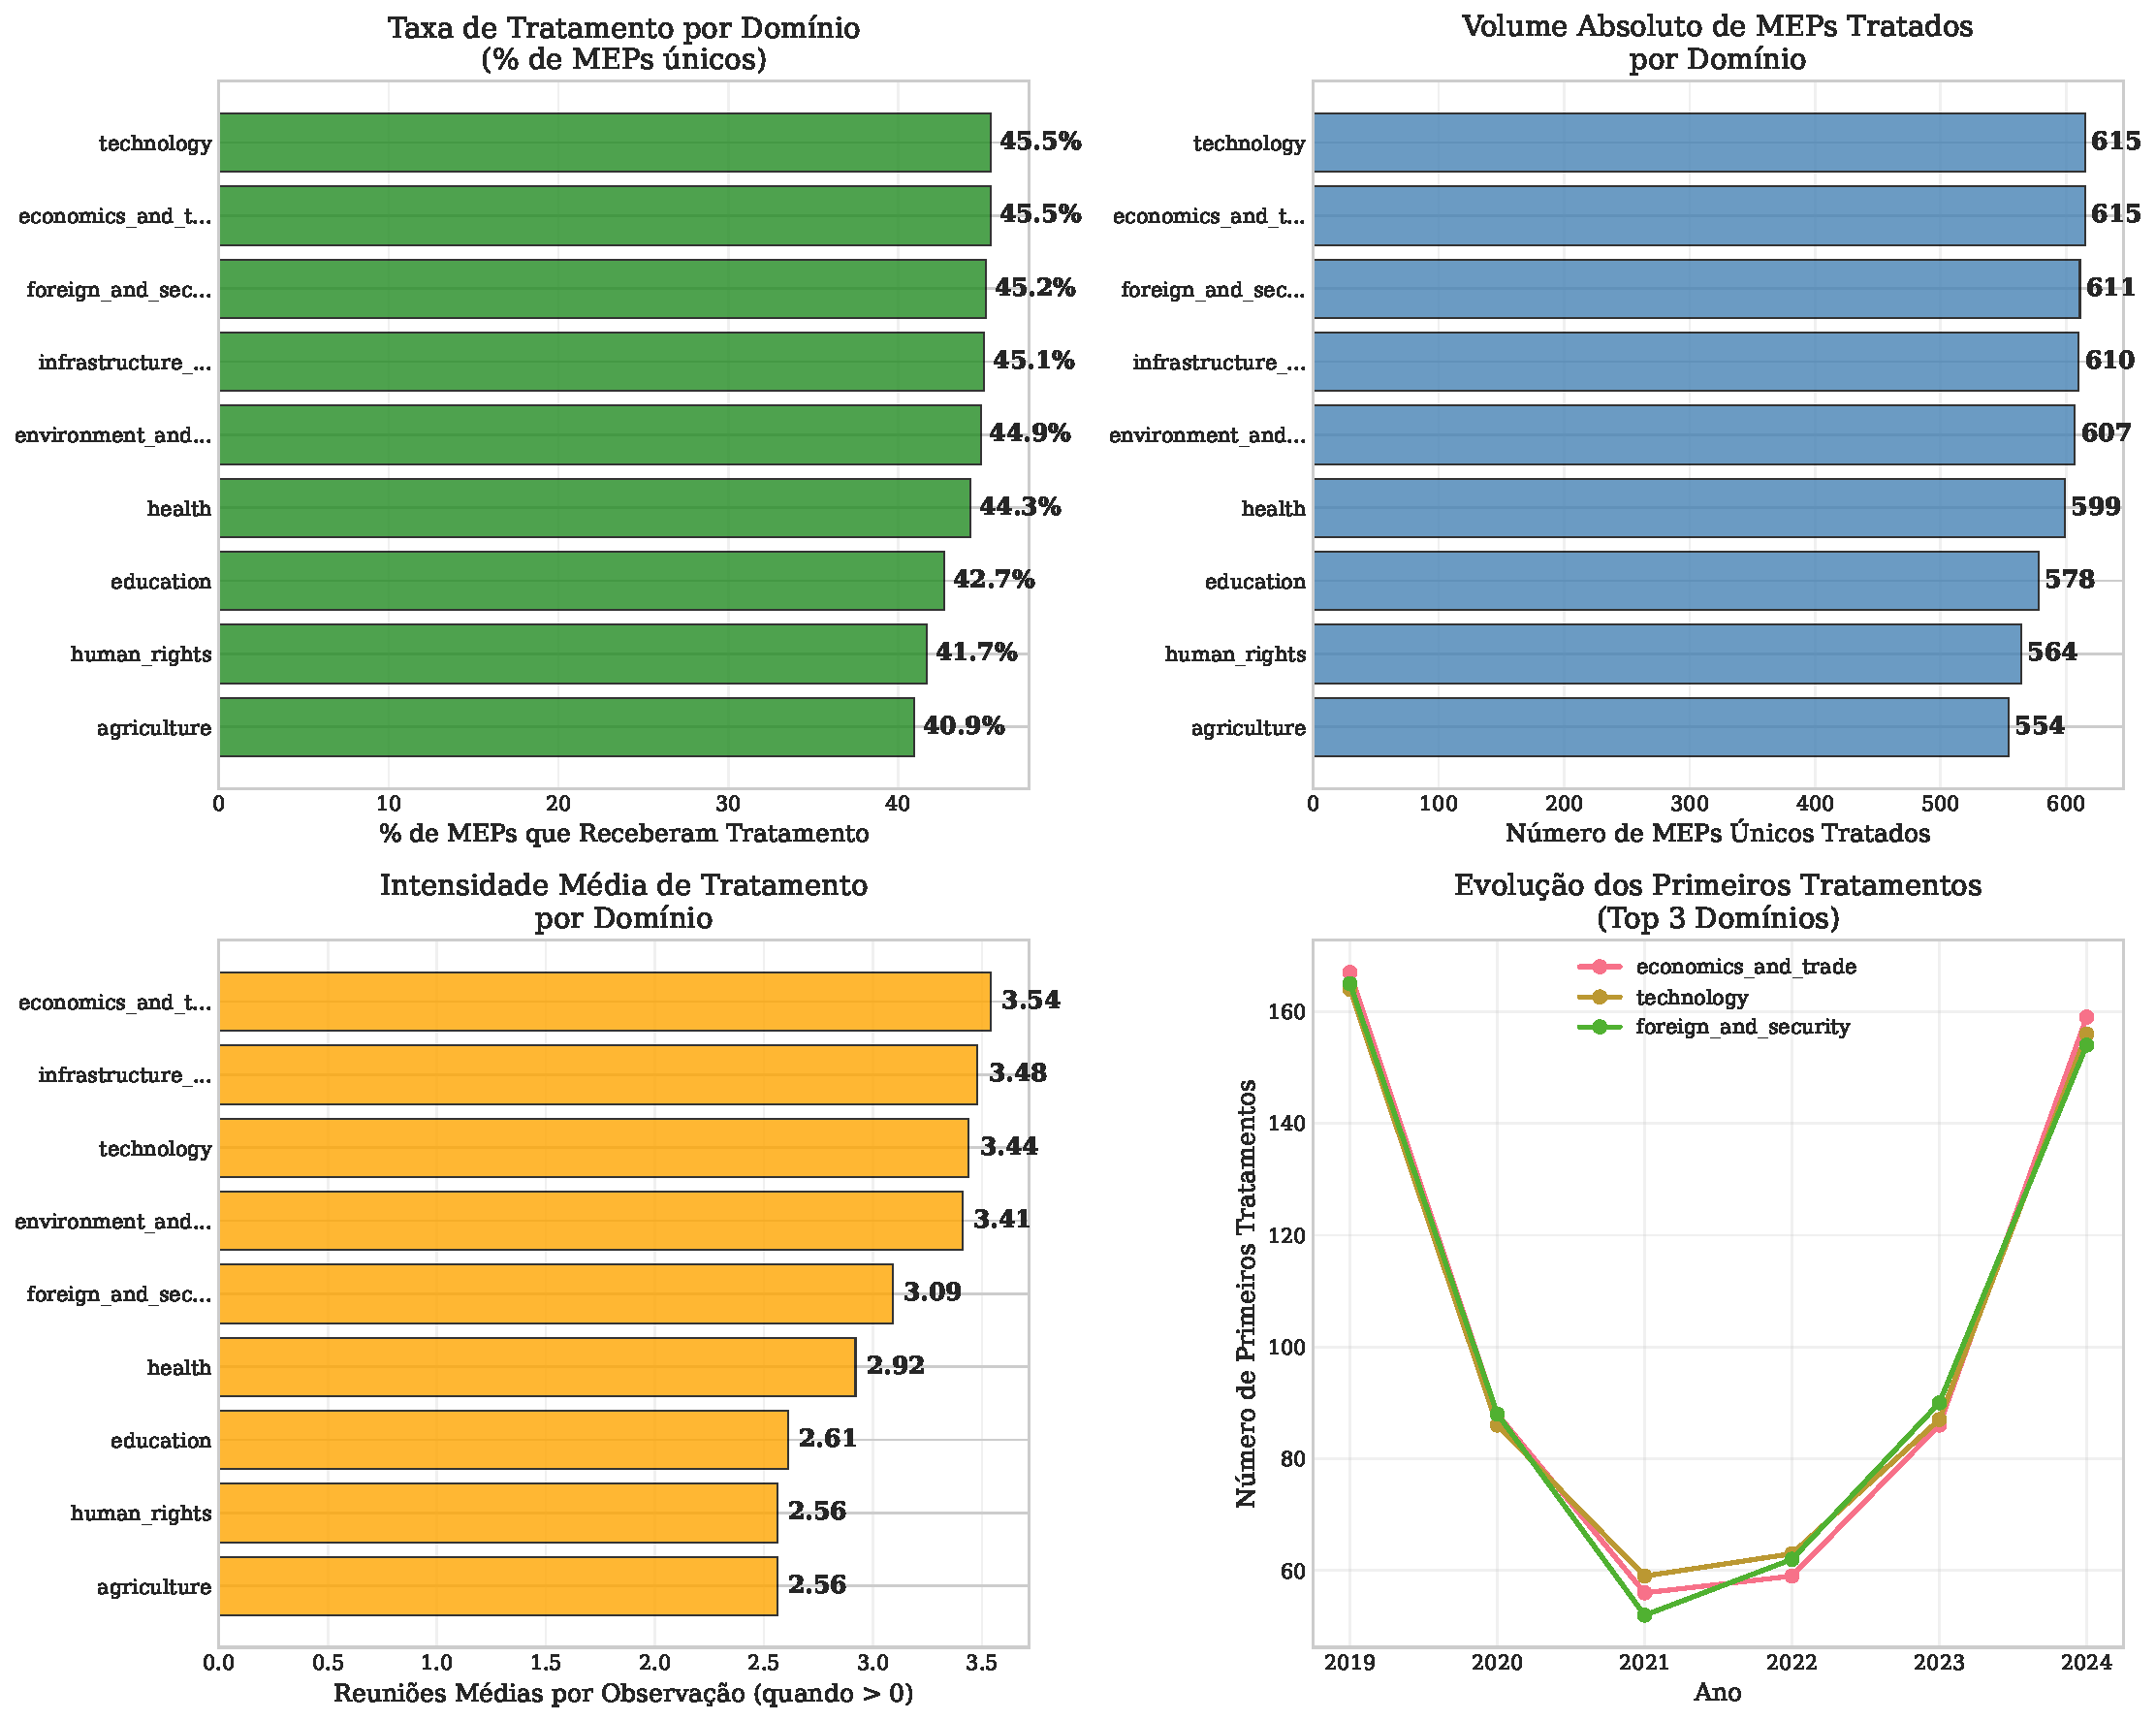
\includegraphics[width=\textwidth]{figures/fig7_domain_treatment_analysis.pdf}
    \caption{Análise detalhada de tratamento por domínio de política pública}
    \label{fig:domain_treatment}
    \note{O painel superior esquerdo mostra a taxa de penetração (percentual de deputados únicos que receberam pelo menos uma reunião em cada domínio). O painel superior direito apresenta o volume absoluto de deputados tratados. O painel inferior esquerdo mostra a intensidade média condicional de tratamento. O painel inferior direito apresenta a evolução temporal dos primeiros tratamentos para os três domínios mais ativos.}
\end{figure}


A heterogeneidade observada entre domínios tem duas implicações metodológicas importantes. Primeiro, a variação sistemática sugere que estimativas de efeito médio podem mascarar diferenças substantivas entre setores, justificando análises de heterogeneidade de efeitos por domínio. Segundo, a ordenação consistente dos domínios por múltiplas métricas (penetração, volume, intensidade) sugere que esta heterogeneidade reflete características estruturais dos setores ao invés de variação aleatória, aumentando a credibilidade de interpretações causais diferenciadas.

% \begin{figure}[htbp]
% \centering
% 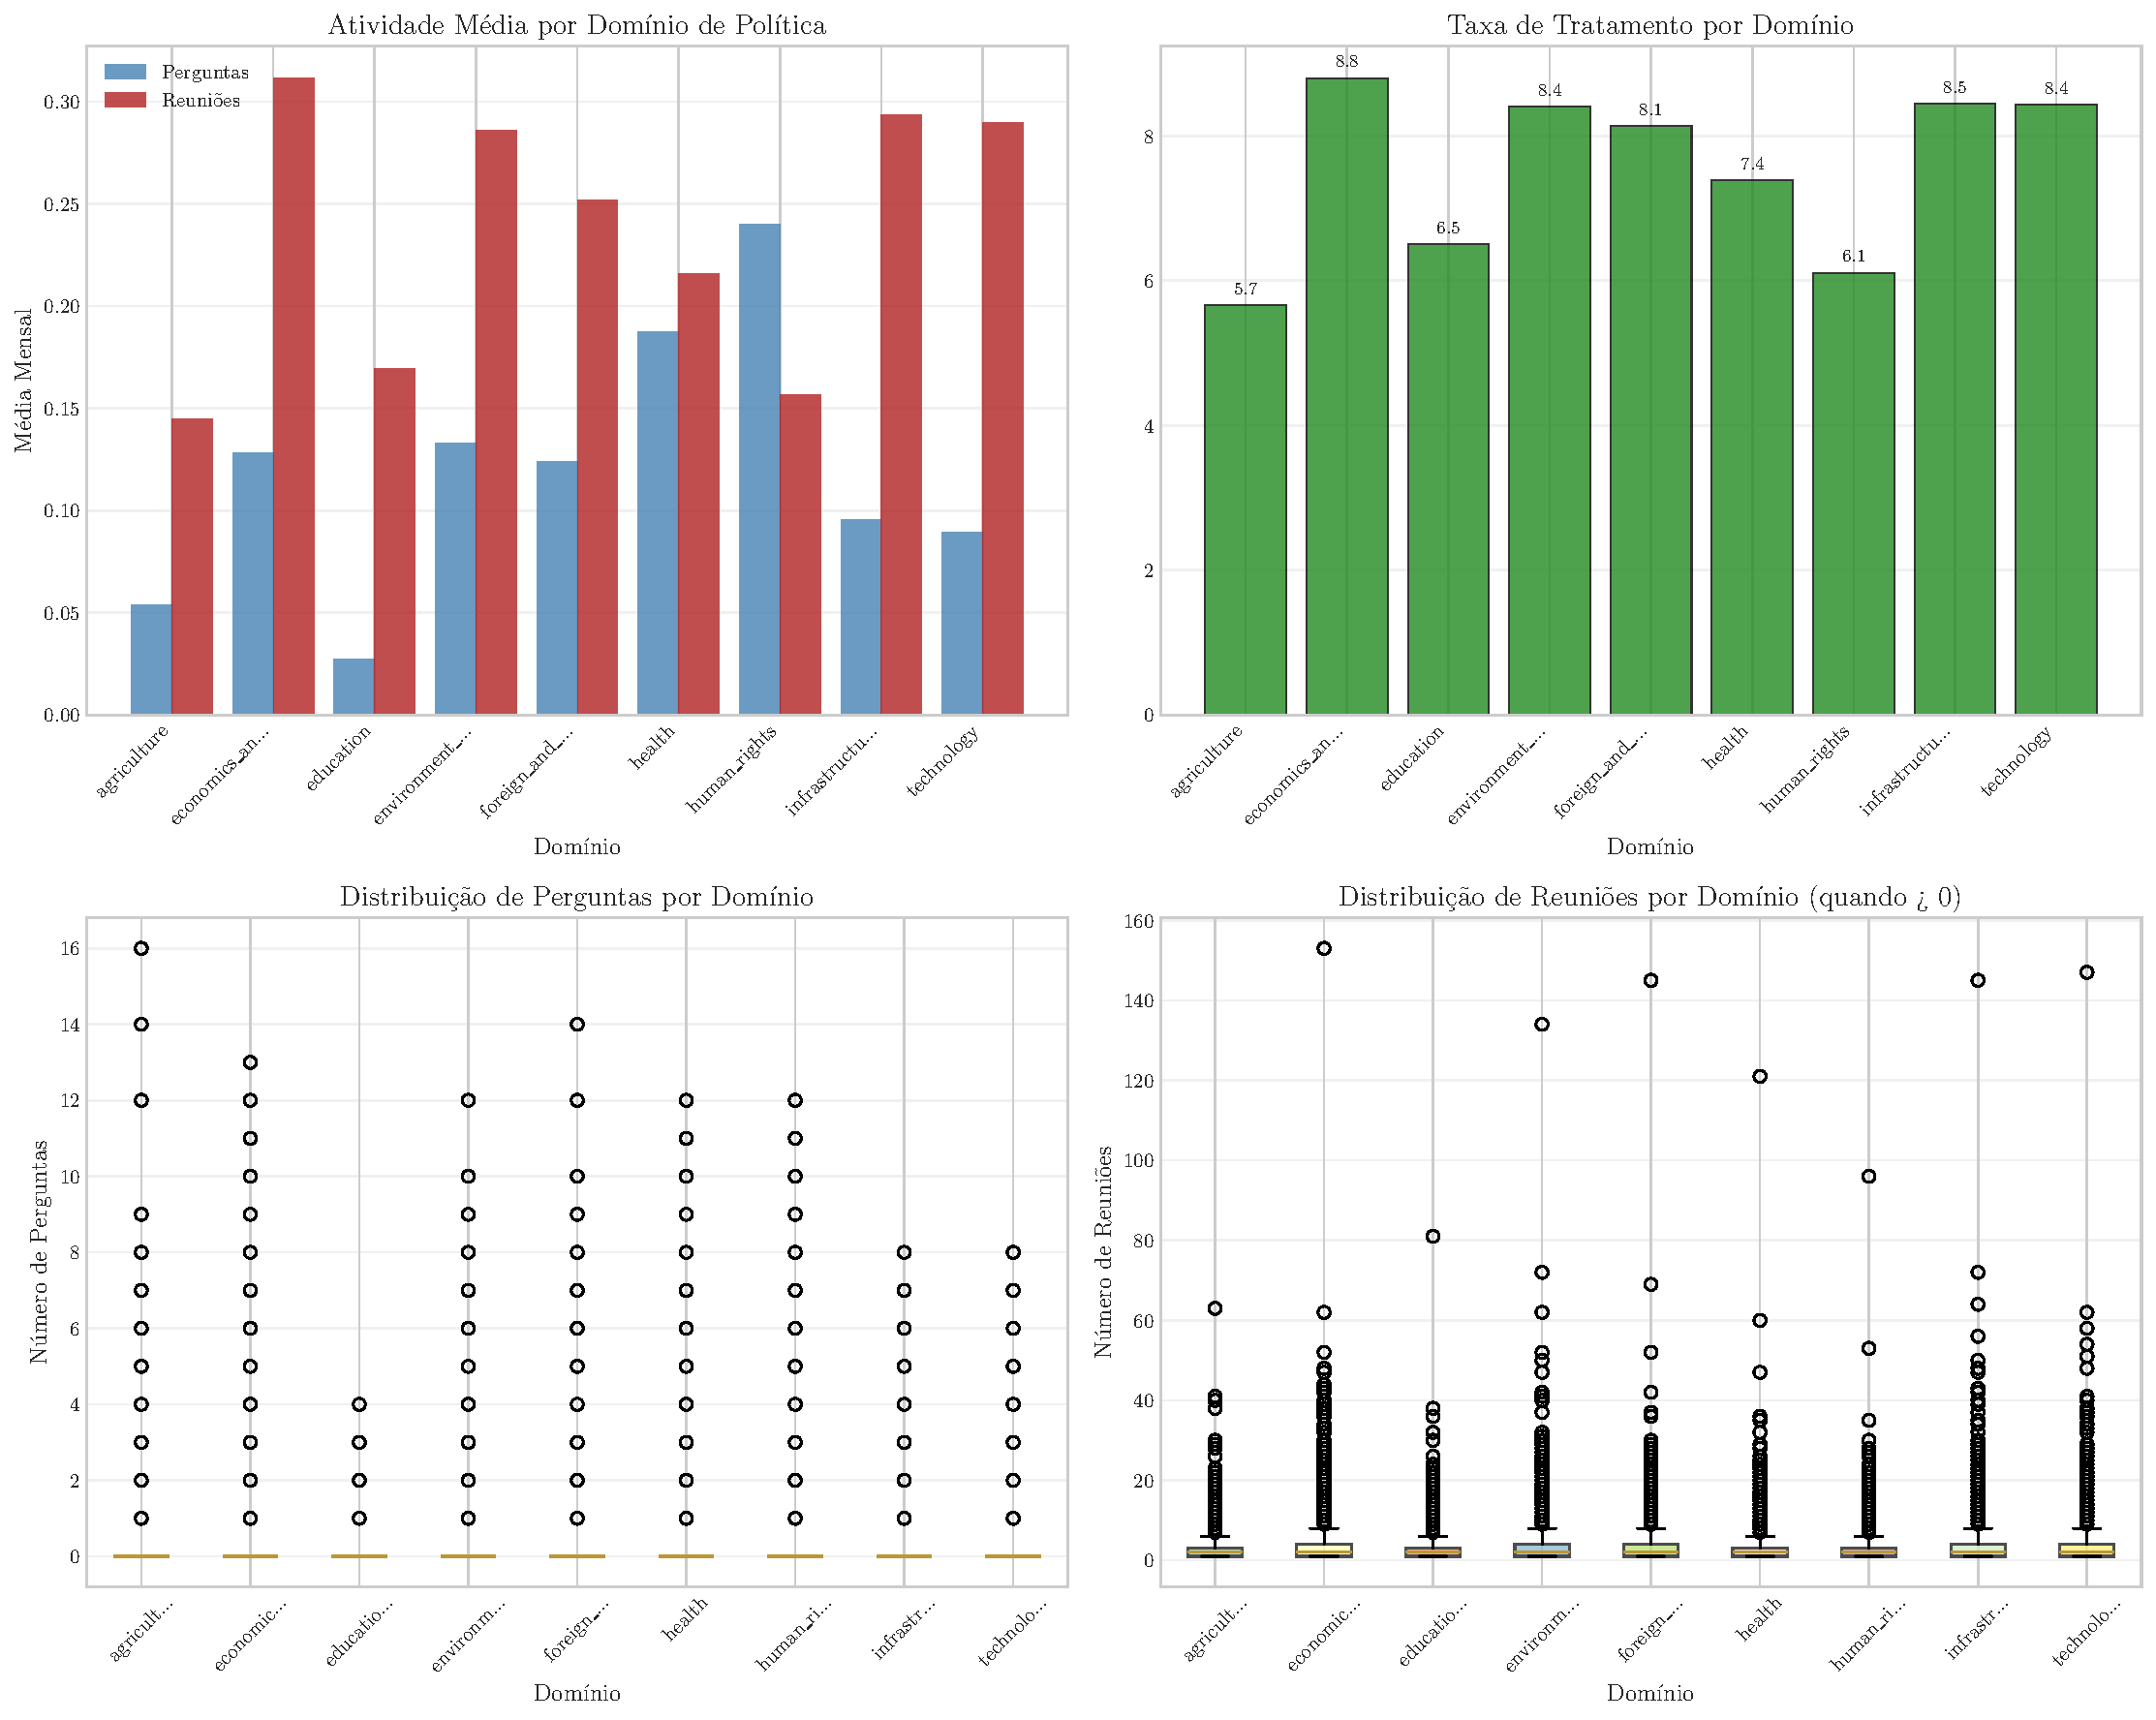
\includegraphics[width=.9\textwidth]{figures/fig3_domain_heterogeneity.pdf}
% \caption{Heterogeneidade por domínio: atividade média e distribuições}
% \label{fig:domain_heterogeneity}
% \note{O painel superior esquerdo mostra a atividade média mensal por domínio para ambas as variáveis. O painel superior direito apresenta as taxas de tratamento mensais. Os painéis inferiores mostram box plots das distribuições completas por domínio, evidenciando tanto diferenças de localização quanto de dispersão entre áreas de política pública.}
% \end{figure}

% \subsection{Análise detalhada: observações MEP-domínio-período}

% Após estabelecer os padrões agregados gerais, temporais e setoriais, esta seção examina as características específicas dos dados no nível mais desagregado: observações MEP-domínio-mês. Esta análise é crucial porque a unidade de observação constitui a base para as estimações econométricas e suas características distribucionais determinam as escolhas metodológicas apropriadas.

% \paragraph{Especialização temática e o problema da inflação artificial de zeros}

A análise da inflação de zeros requer cuidado metodológico particular, pois a unidade de observação MEP-domínio-mês pode gerar inflação \textbf{artificial} de zeros. Como documentado na literatura sobre comportamento parlamentar \cite{example}, deputados tendem a especializar-se tematicamente, concentrando atividade em subconjuntos específicos de domínios. Consequentemente, grupos de interesse, cientes desta especialização, direcionam esforços de lobbying apenas para deputados ativos em suas áreas de interesse.

\textbf{Evidência de especialização temática:} A análise da atividade parlamentar agregada por deputado revela que 97,6\% dos MEPs são \textbf{generalistas} (Índice Herfindahl < 0,4), atuando em média em 7,47 dos 9 domínios disponíveis. Contudo, identificam-se 22 MEPs altamente especializados (HHI > 0,8) que concentram perguntas em domínios únicos, e 26 moderadamente especializados (HHI 0,4-0,8), demonstrando que a especialização, embora limitada, é empiricamente relevante.

\paragraph{Análise corrigida da inflação de zeros}

Para evitar viés na interpretação, a análise da inflação de zeros deve considerar níveis de agregação teoricamente apropriados. A \autoref{tab:zero_inflation_comparison} apresenta uma comparação sistemática entre diferentes níveis de agregação.

\begin{table}[htbp]
\centering
\caption{Inflação de zeros por nível de agregação}
\label{tab:zero_inflation_comparison}
% Usar tabularx para permitir quebra de linha na primeira coluna e evitar overfull hbox
\begin{tabularx}{\textwidth}{>{\raggedright\arraybackslash}X r r r}
\toprule
\textbf{Nível de Agregação} & \textbf{Observações} & \textbf{Zeros Perguntas} & \textbf{Zeros Reuniões} \\
\midrule
MEP-Domínio-Mês (original) & 767{.}151 & 92{,}2\% & 92{,}5\% \\
MEP-Mês (domínios ativos) & 54{.}117 & 70{,}9\% & 85{,}2\% \\
Domínio-Mês (agregado) & 567 & 3{,}2\% & 0{,}0\% \\
\bottomrule
\end{tabularx}
\end{table}

Os resultados revelam que a inflação de zeros é \textbf{sensível ao nível de agregação} e parcialmente \textbf{artificial} quando consideramos especializações temáticas:

\begin{enumerate}
    \item \textbf{Nível MEP-domínio-mês}: A inflação aparentemente extrema (>92\%) reflete em grande parte combinações MEP-domínio onde não se espera atividade sistemática devido à especialização.
    
    \item \textbf{Nível MEP-mês} (agregando apenas domínios onde o MEP demonstra atividade parlamentar): A inflação reduz substancialmente para 70,9\% (perguntas) e 85,2\% (reuniões), revelando que a atividade é \textit{episódica} mas não \textit{ausente}.
    
    \item \textbf{Nível domínio-mês} (agregando todos os MEPs ativos): A inflação torna-se negligível (3,2\% para perguntas, 0\% para reuniões), indicando que há atividade consistente em todos os domínios quando consideramos o conjunto de deputados relevantes.
\end{enumerate}

% A \autoref{fig:corrected_zero_inflation} apresenta uma comparação visual sistemática entre os diferentes níveis de agregação, evidenciando como a especialização temática afeta a interpretação da inflação de zeros.

% \begin{figure}[htbp]
% \centering
% 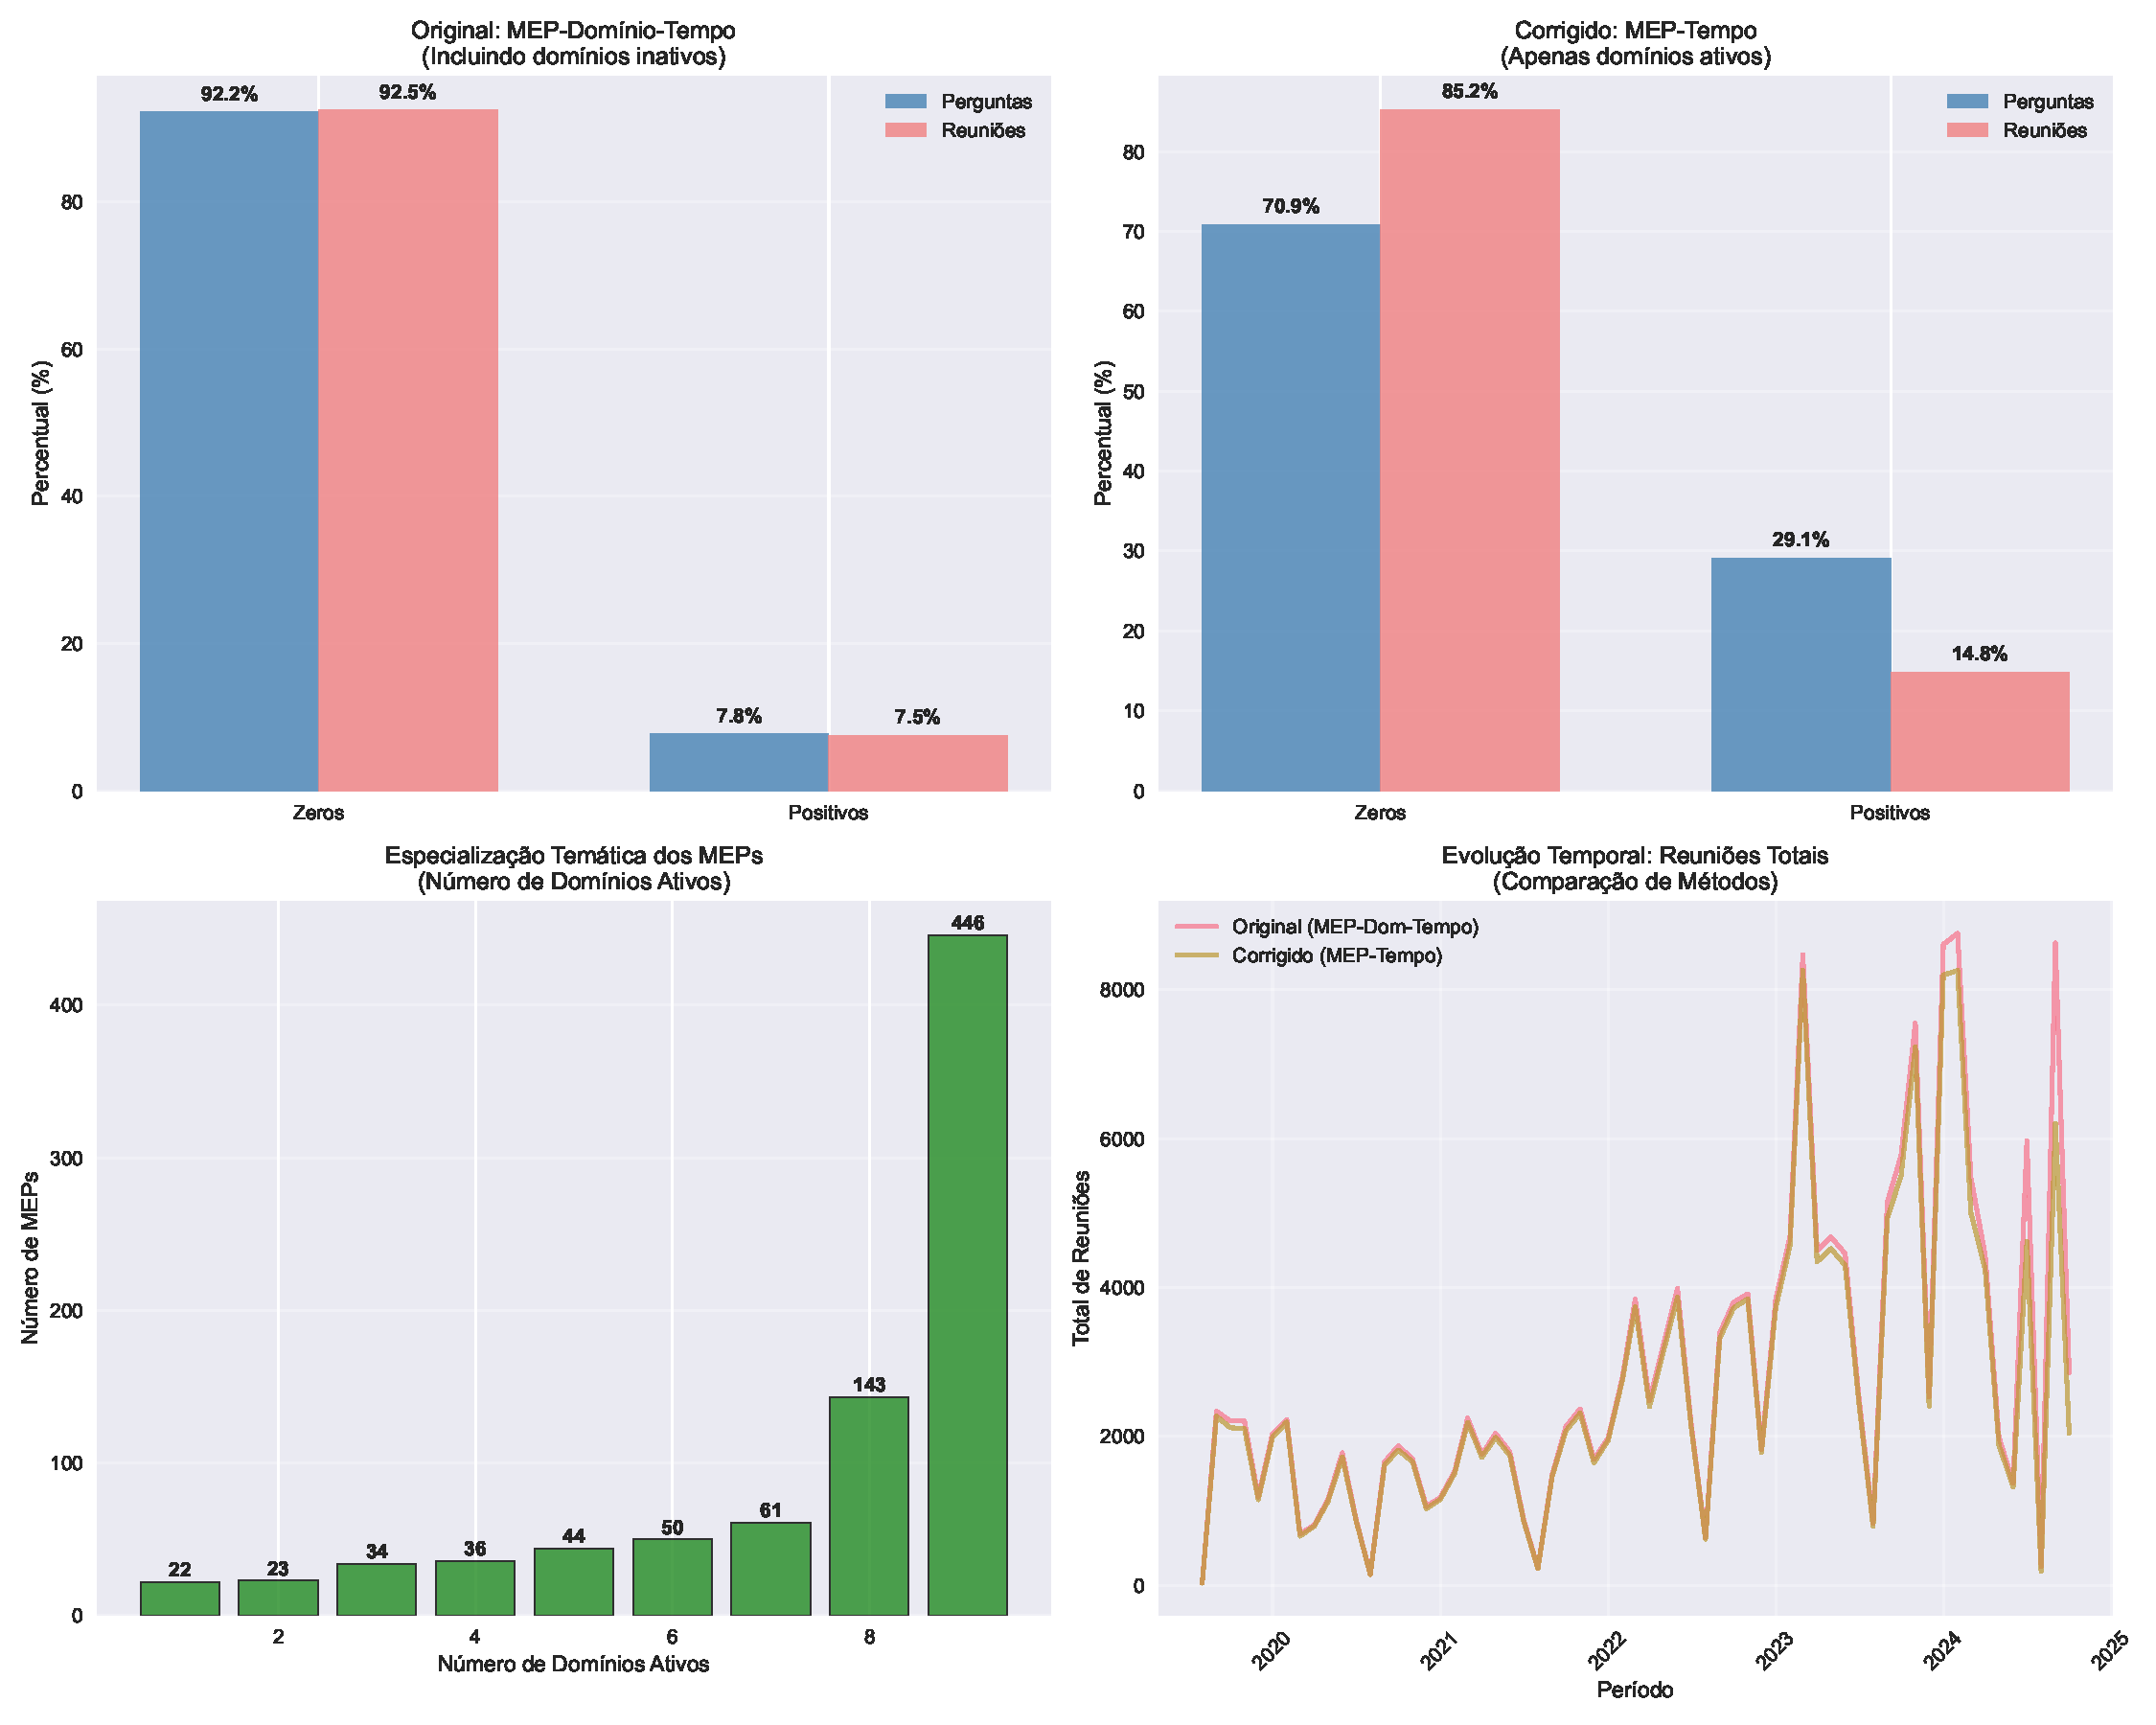
\includegraphics[width=\textwidth]{figures/fig_corrected_zero_inflation_analysis.pdf}
% \caption{Análise corrigida da inflação de zeros considerando especialização temática}
% \label{fig:corrected_zero_inflation}
% \note{O painel superior esquerdo mostra a inflação aparente no nível MEP-domínio-mês original. O painel superior direito apresenta a inflação corrigida no nível MEP-mês considerando apenas domínios ativos. O painel inferior esquerdo mostra a distribuição de especialização temática dos MEPs. O painel inferior direito compara a evolução temporal dos totais mensais entre os métodos original e corrigido.}
% \end{figure}

% \paragraph{Implicações metodológicas revisadas}

Esta análise corrigida tem implicações fundamentais para a estratégia econométrica:

\begin{enumerate}
    \item \textbf{Falso problema de inflação de zeros}: A aparente inflação extrema (>92\%) é em grande parte \textbf{artificial}, resultante da inclusão de combinações MEP-domínio teoricamente implausíveis. A inflação \textbf{real} no nível MEP-mês é substancialmente menor (70,9\%-85,2\%).
    
    \item \textbf{Justificativa para efeitos fixos}: A especialização temática documentada justifica ainda mais fortemente o uso de efeitos fixos MEP×domínio, pois captura heterogeneidade não observada na propensão à atividade em áreas específicas.
    
    \item \textbf{Modelos econométricos apropriados}: Enquanto a inflação moderada (70,9\%) ainda sugere benefícios de modelos de contagem (PPML), a inflação não é tão extrema a ponto de requerer modelos zero-inflated especializados.
    
    \item \textbf{Unidade de análise}: A evidência sustenta a escolha da unidade MEP-domínio-mês para análise causal, pois captura a granularidade necessária para identificação, desde que acompanhada de controles apropriados para especialização.
    
    \item \textbf{Interpretação de resultados}: Efeitos estimados devem ser interpretados condicionalmente à especialização temática, com atenção particular às margens extensiva (entrada em novos domínios) versus intensiva (aumento de atividade em domínios existentes).
\end{enumerate}

% \paragraph{Decomposição em margens extensiva e intensiva}

% A extrema inflação de zeros torna analiticamente vantajoso decompor o fenômeno em duas margens conceituais distintas: a \textbf{margem extensiva} (decisão de participar) e a \textbf{margem intensiva} (nível de atividade condicional à participação). Esta decomposição é teoricamente relevante porque diferentes mecanismos causais podem operar em cada margem.

% A \autoref{fig:extensive_intensive} apresenta uma análise detalhada desta decomposição, incluindo a sobreposição entre atividades parlamentares e de lobbying.

% \begin{figure}[htbp]
% \centering
% 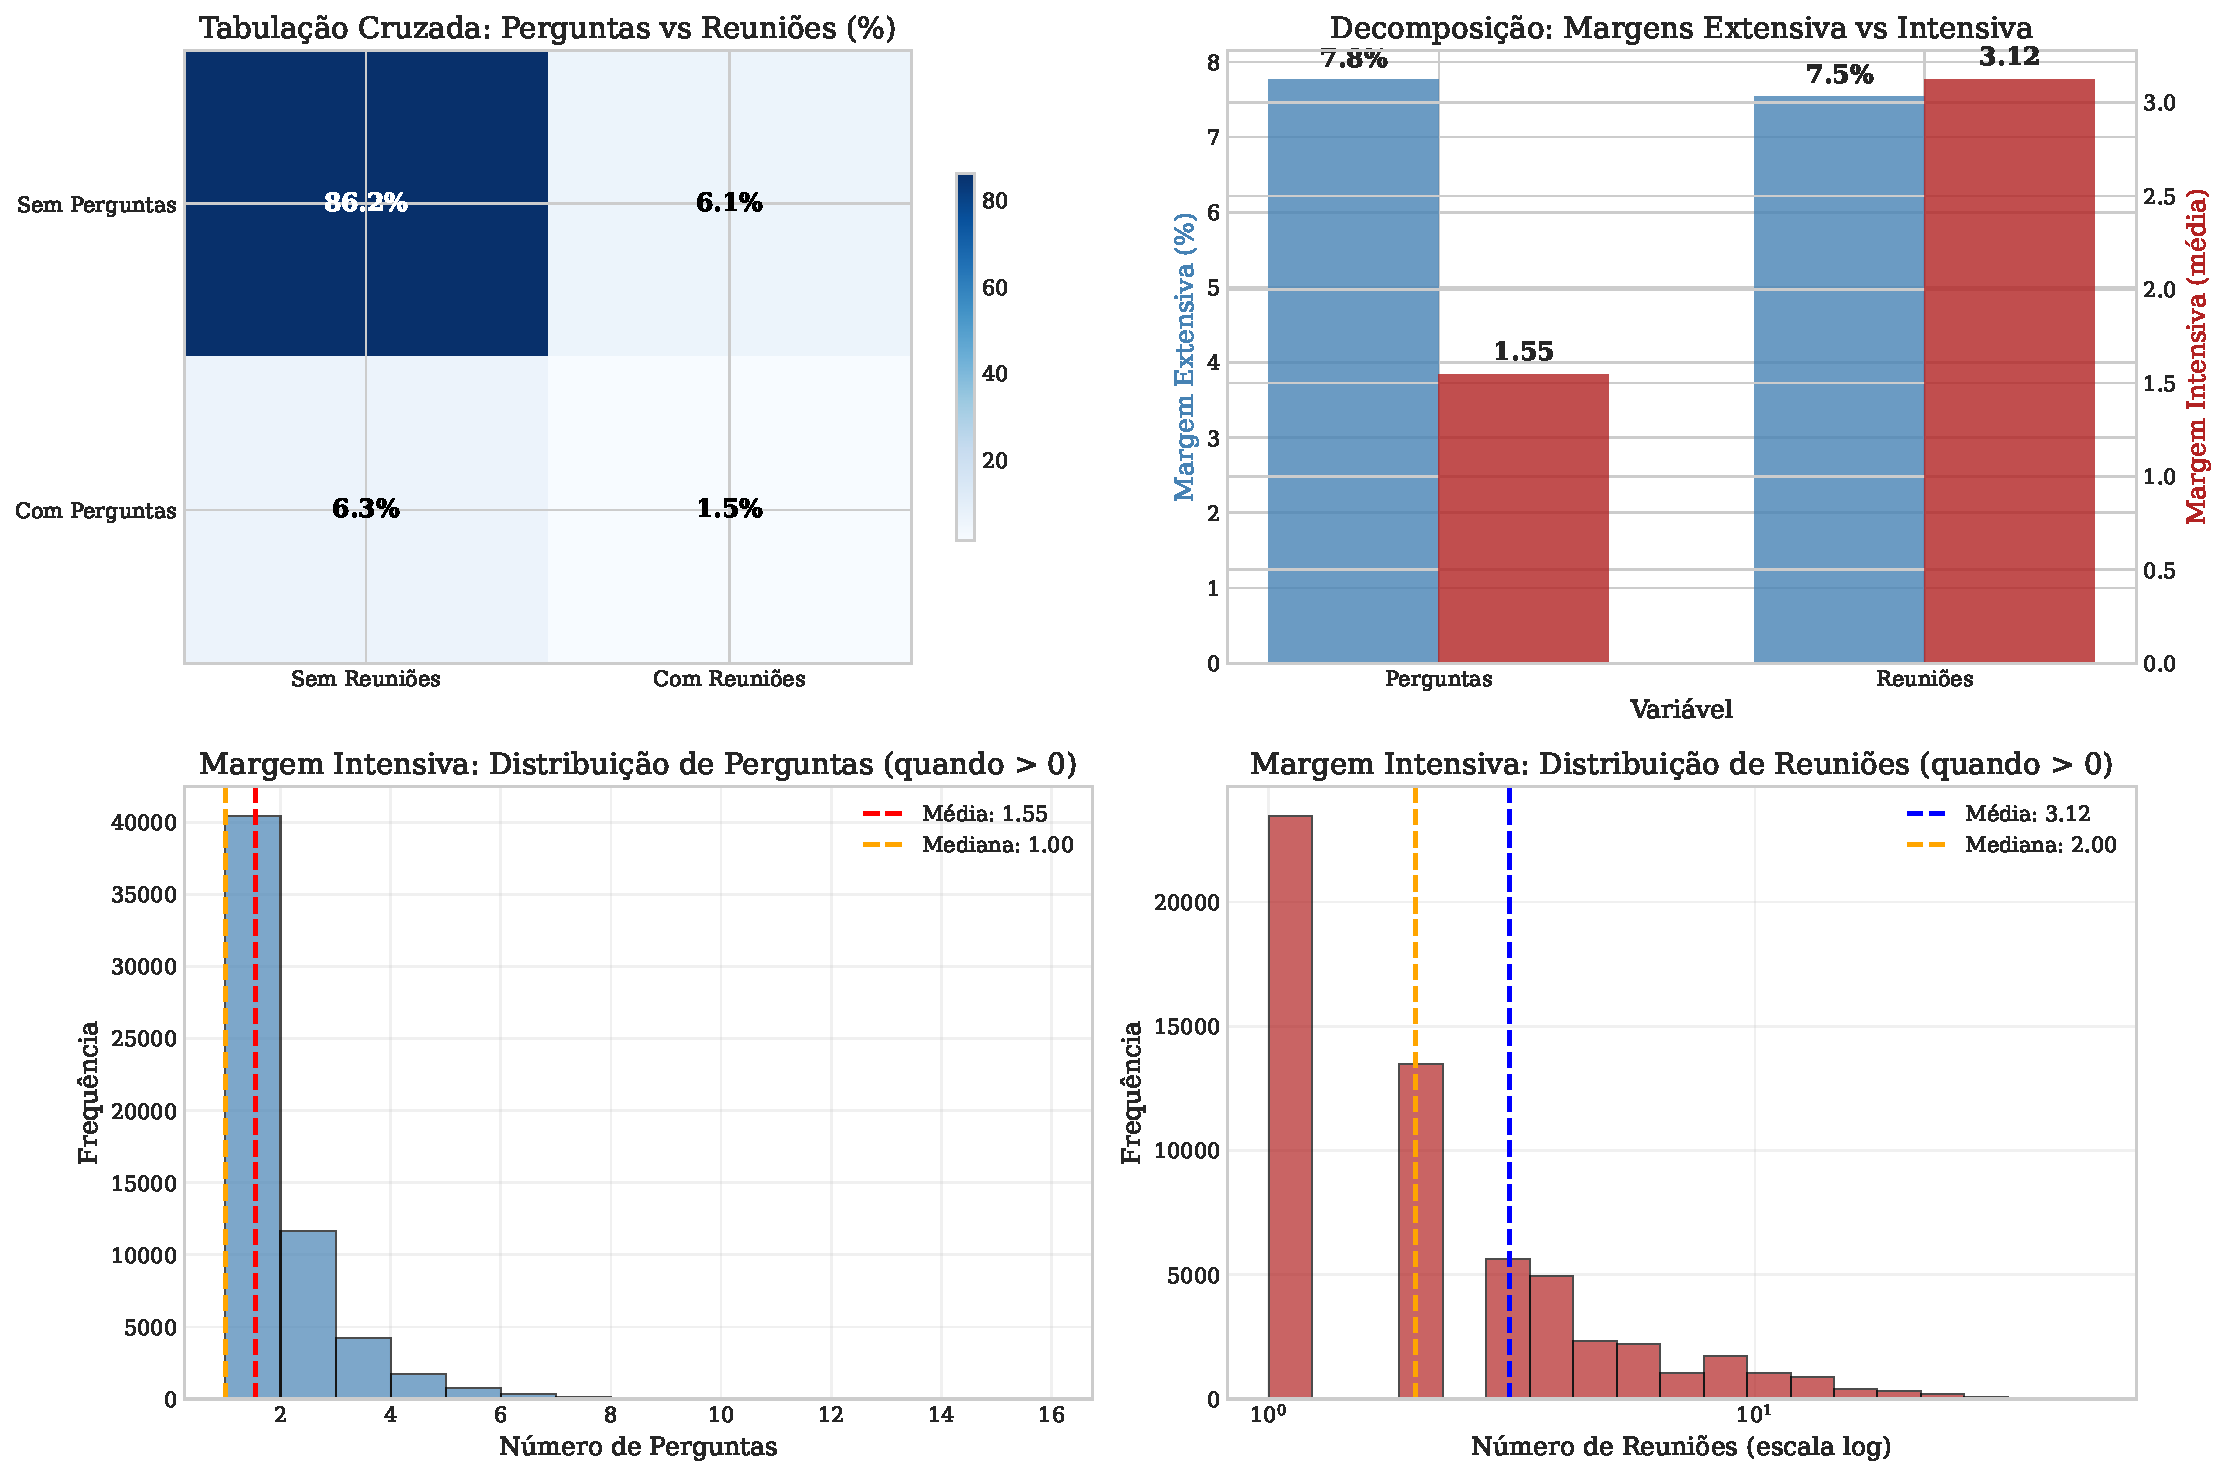
\includegraphics[width=\textwidth]{figures/fig5_extensive_intensive_margins.pdf}
% \caption{Análise das margens extensiva e intensiva}
% \label{fig:extensive_intensive}
% \note{O painel superior esquerdo apresenta a tabulação cruzada entre atividade parlamentar e de lobbying, revelando padrões de sobreposição. O painel superior direito decompõe as margens extensiva (participação) e intensiva (intensidade condicional). Os painéis inferiores mostram as distribuições condicionais completas para ambas as variáveis na margem intensiva.}
% \end{figure}

% A tabulação cruzada revela um padrão notável: apenas \textbf{0,4\%} das observações apresentam simultaneamente perguntas parlamentares e reuniões de lobbying. Esta baixa sobreposição indica que atividade parlamentar e lobbying são largamente \textbf{independentes} no nível temporal mensal, sugerindo que potenciais efeitos causais podem operar através de canais indiretos ou com defasagens temporais que não são captadas na correlação contemporânea.

% Na margem extensiva, 7,8\% das observações apresentam atividade parlamentar e 7,5\% apresentam atividade de lobbying. Na margem intensiva, condicionalmente à participação, as médias são 1,54 perguntas e 3,15 reuniões por observação, com distribuições altamente assimétricas evidenciando concentração mesmo dentro do subconjunto de observações ativas.

% \paragraph{Correlações e relações entre variáveis}

% Para completar a caracterização dos dados, a \autoref{fig:correlation_analysis} examina as relações diretas entre as variáveis principais através de múltiplas perspectivas analíticas.

% \begin{figure}[htbp]
% \centering
% 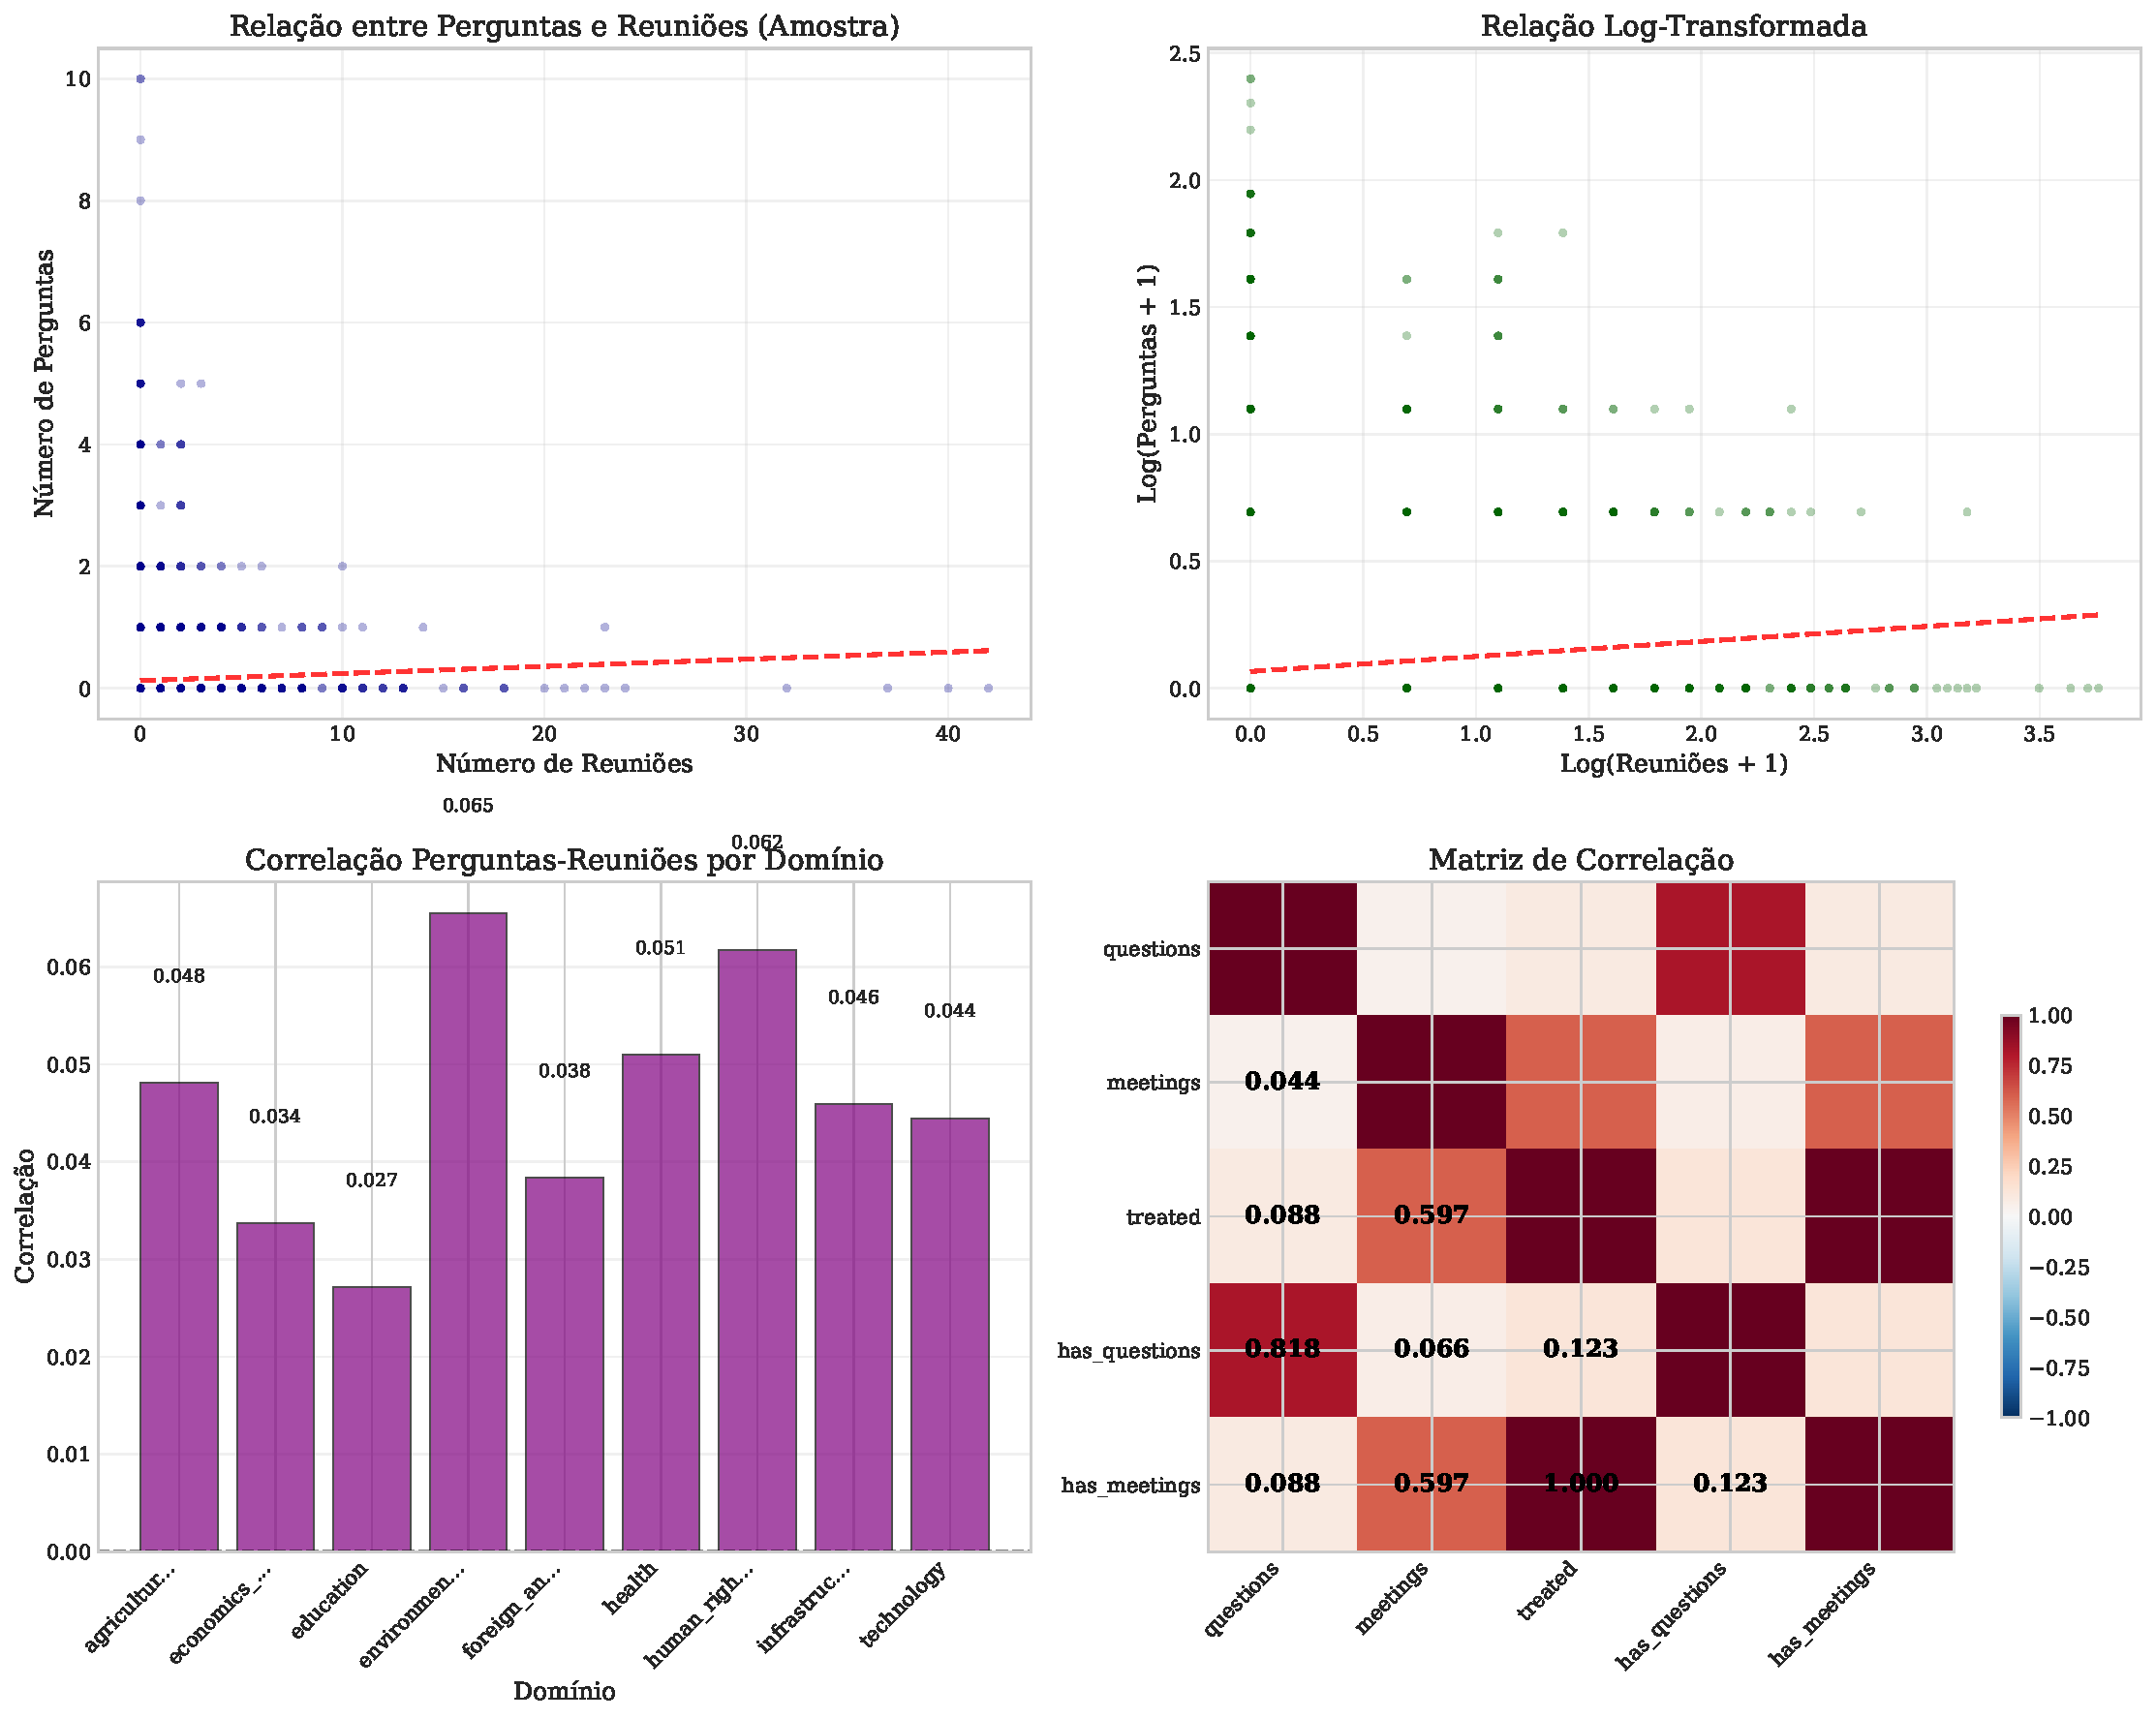
\includegraphics[width=\textwidth]{figures/fig4_correlation_analysis.pdf}
% \caption{Análise de correlações e relações entre variáveis}
% \label{fig:correlation_analysis}
% \note{O painel superior esquerdo mostra a relação geral entre perguntas e reuniões no nível MEP-domínio-mês. O painel superior direito apresenta a mesma relação em escala logarítmica. O painel inferior esquerdo mostra as correlações por domínio. O painel inferior direito apresenta a matriz de correlação entre as variáveis principais.}
% \end{figure}

% A análise de correlações revela padrões consistentes com a baixa sobreposição contemporânea observada anteriormente. No nível agregado MEP-domínio-mês, a correlação é positiva mas modesta. Interessantemente, existe heterogeneidade sistemática nas correlações entre domínios, sugerindo que a força da relação varia com características setoriais específicas.

\subsection{Síntese e implicações metodológicas}

A análise descritiva multinível revela um conjunto coerente de \textit{stylized facts} que informam tanto a compreensão teórica quanto as escolhas metodológicas para a análise causal subsequente.

% \paragraph{Características empíricas principais}

Primeiro, o \textbf{lobbying é um fenômeno disseminado mas episódico}. Enquanto 46,3\% dos deputados recebem lobbying durante o período estudado, a atividade temporal é concentrada: considerando apenas domínios onde MEPs demonstram atividade parlamentar, 70,9\% das observações MEP-mês não apresentam perguntas e 85,2\% não apresentam reuniões, indicando que a influência opera através de interações concentradas temporalmente.

Segundo, existe \textbf{concentração extrema} em múltiplas dimensões. No nível individual, a distribuição de reuniões é altamente assimétrica (mediana 105, média 288, máximo 4.274). Crucialmente, a aparente inflação extrema de zeros (>92\%) no nível MEP-domínio-mês é em grande parte artificial, refletindo combinações onde não se espera atividade devido à especialização temática.

Terceiro, observa-se \textbf{heterogeneidade sistemática entre domínios} em todas as métricas analisadas. Domínios de regulação econômica apresentam consistentemente maior atividade de lobbying, refletindo diferenças estruturais em stakes econômicos e capacidade organizacional. Esta heterogeneidade é consistente com a especialização temática documentada.

Quarto, a \textbf{especialização temática é limitada mas empiricamente relevante}: enquanto 97,6\% dos MEPs atuam como generalistas (HHI < 0,4), existem 22 deputados altamente especializados e 26 moderadamente especializados, com padrões claros de concentração que informam estratégias de lobbying e justificam controles econométricos específicos.

Quinto, a \textbf{correlação contemporânea entre lobbying e atividade parlamentar é baixa} no nível temporal mensal, mas padrões agregados sugerem relações mais complexas que podem envolver defasagens temporais ou mecanismos indiretos.

% \paragraph{Implicações para estratégia econométrica}

Estas características empíricas têm implicações diretas para a escolha da estratégia econométrica:

\begin{enumerate}
    \item \textbf{Especificação funcional}: A inflação moderada de zeros (70,9\%-85,2\% após correção) e natureza de contagem das variáveis justificam o uso de estimadores Poisson Pseudo-Maximum Likelihood (PPML), mas não requerem modelos zero-inflated especializados.
    
    \item \textbf{Estrutura de efeitos fixos}: A evidência de especialização temática justifica fortemente efeitos fixos MEP×domínio para controlar heterogeneidade não observada na propensão à atividade em áreas específicas, complementados por efeitos fixos temporais.
    
    \item \textbf{Correção de viés de seleção}: A especialização temática implica que observações MEP-domínio-mês com probabilidade zero de atividade podem distorcer estimativas. Controles ou exclusões baseadas em atividade histórica podem ser apropriados.
    
    \item \textbf{Estrutura de erros}: A concentração temporal da atividade e especialização justificam erros-padrão agrupados no nível MEP×domínio para capturar correlação serial específica por área de atuação.
    
    \item \textbf{Análise de heterogeneidade}: A variação sistemática entre domínios, combinada com especialização, justifica análises diferenciadas por setor e investigação de efeitos nas margens extensiva (entrada em novos domínios) versus intensiva.
    
    \item \textbf{Interpretação causal}: Efeitos estimados devem ser interpretados condicionalmente à especialização temática existente, distinguindo entre expansão de atividade em domínios familiares versus diversificação para novas áreas.
\end{enumerate}

Finalmente, a \textbf{estrutura balanceada do painel} e a \textbf{cobertura temporal substancial} fornecem condições ideais para estratégias de identificação baseadas em variação temporal within-individual, maximizando o poder estatístico while minimizando preocupações com confounding não observado time-invariant.

Esta análise descritiva abrangente estabelece as bases empíricas sólidas para a estratégia de identificação causal apresentada na seção seguinte, demonstrando que os dados possuem as características necessárias para investigar rigorosamente os efeitos do lobbying na atividade parlamentar dos deputados europeus.

% !TeX root = ../../main.tex
\section{Análise de efeitos do lobby}
\label{sec:resultados_efeitos}

Optamos por estimar modelos de contagem via \acrshort{ppml} com \textit{link} logaritmo por três razões principais. Primeiro, as variáveis de interesse (perguntas e reuniões) são contagens, com forte assimetria e alta incidência de zeros no nível MEP–domínio–mês. O \acrshort{ppml} lida naturalmente com zeros sem exigir transformações logarítmicas \textit{ad hoc} que descartam observações. Segundo, o \acrshort{ppml} é consistente sob especificação correta da média condicional mesmo na presença de sobredispersão e heterocedasticidade não especificada, fornecendo erros-padrão robustos quando combinados com \textit{clustering}. Terceiro, a implementação com efeitos fixos de alta dimensão é estável e amplamente utilizada na literatura aplicada (estimador \texttt{fepois} do pacote \texttt{fixest}).

No \acrshort{ppml} com \textit{link} log, a expectativa condicional é \(\mathbb{E}[y\mid X] = \exp(X\beta)\). Assim, para um regressor contínuo \(x_k\) (por exemplo, \textit{meetings} em nível), o coeficiente \(\beta_k\) tem interpretação multiplicativa: um aumento de uma unidade em \(x_k\) está associado a uma variação percentual de \(100\times(\mathrm{e}^{\beta_k}-1)\%\) na média de \(y\), \textit{ceteris paribus}.

A especificação segue o \textit{framework} analítico delineado no capítulo: controlamos por heterogeneidade não observada ao nível do membro e por choques comuns estruturados por partido, país e domínio ao longo do tempo. Concretamente, estimamos modelos com efeitos fixos de membro (\texttt{member\_id}) e efeitos fixos tempo-variantes por país (\texttt{country\_time}), por partido (\texttt{party\_time}) e por domínio (\texttt{domain\_time}). Os erros-padrão são agrupados em \textit{domínio×tempo} e \textit{membro}, capturando correlação serial e choques idiossincráticos nesse nível, conforme implementado nos scripts empíricos.

Essa modelagem garante três propriedades fundamentais para a identificação dos efeitos: (i) permite comparar a evolução da atividade do mesmo \acrshort{mpe} ao longo do tempo, controlando por características não observadas e invariantes como preferências individuais, capital político e produtividade; (ii) elimina a influência de choques ou tendências comuns a todos os \acrshort{mpe}s de um mesmo país ou partido em cada mês, por meio dos efeitos fixos específicos de país$\times$tempo e partido$\times$tempo; e (iii) assegura robustez frente a choques específicos de cada setor ou área temática ao incorporar efeitos fixos de domínio$\times$tempo (\texttt{domain\_time}), isolando variações idiossincráticas desses contextos.

Para testar a Hipótese 1, utilizamos o painel agregado MEP–domínio–mês em amostra combinada (\textit{pooled}) e estimamos PPML com a estrutura de efeitos fixos descrita acima. O coeficiente associado às reuniões (\textit{meetings}) é \textbf{positivo}, indicando que aumentos na intensidade de lobbying estão associados a maior atividade parlamentar em termos de perguntas. Esse resultado é consistente em especificações alternativas, incluindo a versão com termo quadrático para capturar possíveis não linearidades e a inclusão de efeitos fixos \textit{domínio×tempo}, sugerindo robustez do sinal e da magnitude qualitativa do efeito.

Em termos de interpretação, mantidos constantes os efeitos fixos, um incremento marginal em reuniões está associado a um aumento proporcional na média de perguntas dado por \(\mathrm{e}^{\hat{\beta}}-1\). Reportamos os efeitos como variações percentuais estimadas na seção de tabelas de resultados, com intervalos de confiança baseados em erros-padrão agrupados.

\begin{table}[htbp]
\centering
\caption{Resumo dos modelos \acrshort{ppml} para a Hipótese 1}
\label{tab:ppml_h1_both}
\begin{tabularx}{\textwidth}{>{\raggedright\arraybackslash}p{.22\textwidth} >{\raggedright\arraybackslash}X >{\raggedright\arraybackslash}X}
\toprule
  & PPML & PPML (Quad.) \\
\midrule
Reuni\~oes & 0.013*** (0.002) & 0.037*** (0.005) \\
Reuni\~oes$^2$ &  & -0.001*** (0.000) \\
\midrule
Observa\c{c}\~oes & 711,855 & 711,855 \\
Efeitos fixos & \multicolumn{2}{p{.72\textwidth}}{\raggedright pa\'is$\times$tempo; partido$\times$tempo; dom\'inio$\times$tempo} \\
Cluster & \multicolumn{2}{p{.72\textwidth}}{\raggedright dom\'inio$\times$tempo; membro} \\
\bottomrule
\end{tabularx}

\note{A coluna ``PPML'' reporta o modelo principal com efeito linear em \textit{meetings}. A coluna ``PPML (Quadrático)'' adiciona \(\textit{meetings}^2\) para capturar retornos marginais decrescentes. Efeitos fixos: membro; país$\times$tempo; partido$\times$tempo. Erros-padrão agrupados em domínio$\times$tempo e membro.}
\end{table}

\begin{figure}[htbp]
\centering
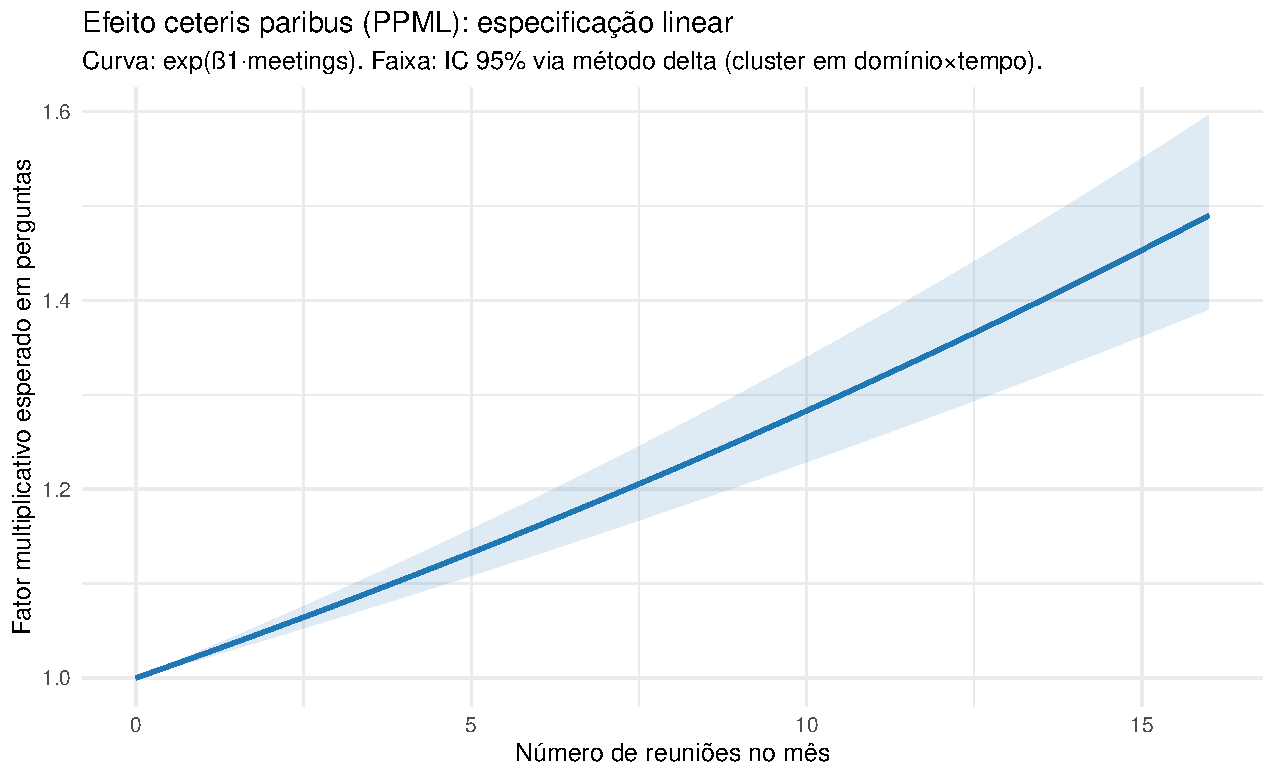
\includegraphics[width=\textwidth]{figures/h1_test/fig_effect_linear_ppml.pdf}
\caption{Efeito esperado ceteris paribus: especificação linear (\acrshort{ppml})}
\label{fig:effect_linear_ppml}
\note{A curva apresenta o fator multiplicativo esperado em perguntas como função do número de reuniões no mês, mantendo constantes os efeitos fixos (\(\exp(\hat{\beta}_1\cdot \textit{meetings})\)). A faixa sombreada corresponde ao intervalo de 95\% obtido via método delta com erros-padrão agrupados em domínio×tempo.}
\end{figure}

\begin{figure}[htbp]
\centering
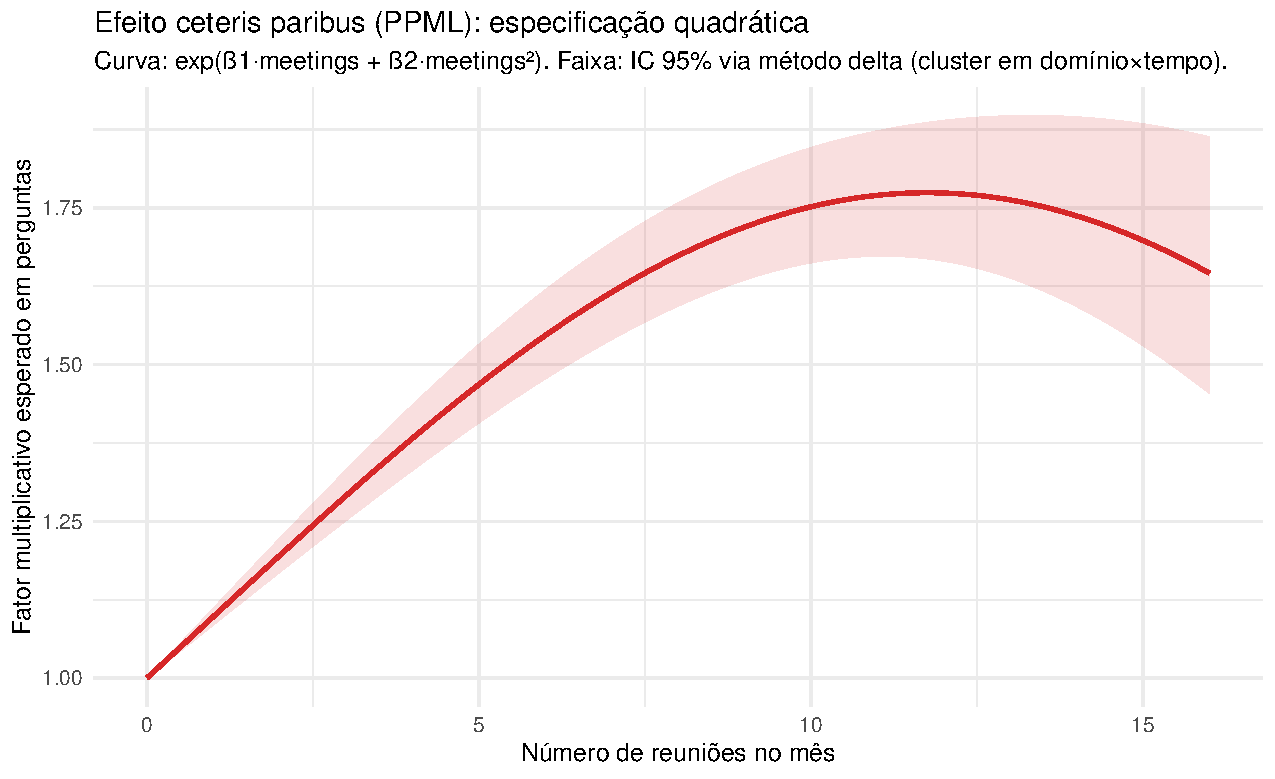
\includegraphics[width=\textwidth]{figures/h1_test/fig_effect_quadratic_ppml.pdf}
\caption{Efeito esperado ceteris paribus: especificação quadrática (\acrshort{ppml})}
\label{fig:effect_quadratic_ppml}
\note{A curva apresenta o fator multiplicativo esperado em perguntas como função do número de reuniões, permitindo retornos marginais decrescentes (\(\exp(\hat{\beta}_1\cdot \textit{meetings} + \hat{\beta}_2\cdot \textit{meetings}^2)\)). A faixa sombreada representa o IC de 95\% via método delta com a matriz de variância-covariância agrupada.}
\end{figure}

\autoref{tab:ppml_h1_both} mostra que o coeficiente de \textit{meetings} no modelo \acrshort{ppml} linear é positivo e estatisticamente significativo, evidenciando que aumentos na intensidade de lobbying associam-se a maior número de perguntas, \textit{ceteris paribus}. Na especificação quadrática, o termo linear permanece positivo enquanto o termo quadrático é negativo, indicando retornos marginais decrescentes: o impacto adicional de reuniões sobre perguntas diminui à medida que o volume de reuniões cresce.

Essa interpretação decorre da forma funcional do \acrshort{ppml} (\(\mathbb{E}[y\mid X]=\exp(X\beta)\)). No modelo linear, um acréscimo de uma unidade em \textit{meetings} altera a média condicional de perguntas em \(100\times(\mathrm{e}^{\hat{\beta}_1}-1)\%\). No modelo quadrático, o efeito marginal em log-média é \(\partial\log\mathbb{E}[y\mid X]/\partial\,\textit{meetings}=\hat{\beta}_1+2\hat{\beta}_2\,\textit{meetings}\). Com \(\hat{\beta}_2<0\), esse efeito declina com o nível de \textit{meetings}, isto é, há retornos marginais decrescentes. 

Em particular, a magnitude do termo quadrático é muito inferior ao efeito linear (0,098 vs. 0,004), o que indica retornos marginais decrescentes pequenos na faixa observada. Isso implica que atores com maior disponibilidade de recursos enfrentam pouca perda de eficácia ao intensificar o número de reuniões e, portanto, podem sustentar níveis muito mais altos de lobbying; tal padrão é consistente com a hipótese de que grandes players conseguem alavancar sua capacidade financeira para obter influência relativamente maior, mesmo diante de retornos marginais decrescentes.

% importante mencionar que esse efeito esperado é considerando o número de reuniões com apenas um parlamentar dentro de um único mês. Não considera o efeito total das reuniões que podem ser realizadas em meses diferentes. Não captura a dinâmica de uma organização realizar diversas reuniões com diversos parlamentares em meses diferents. Essa análise foi realizada para testar as hipóteses 2 e 3.

As curvas em \autoref{fig:effect_linear_ppml} e \autoref{fig:effect_quadratic_ppml} tornam essa dinâmica visual. A primeira apresenta um efeito multiplicativo crescente de forma monotônica (\(\exp(\hat{\beta}_1\,\allowbreak\textit{meetings})\)), com faixas de incerteza (IC 95\%) obtidas por método delta usando a matriz de variância-covariância com \textit{clustering} em domínio$\times$tempo e membro. A segunda permite curvatura (\(\exp(\hat{\beta}_1\,\allowbreak\textit{meetings}+\hat{\beta}_2\,\allowbreak\textit{meetings}^2)\)) e revela concavidade compatível com saturação de agenda: para níveis altos de \textit{meetings}, o ganho marginal em perguntas é menor. Em ambas as figuras, o eixo horizontal é mantido dentro do suporte observado dos dados para evitar extrapolações.

Do ponto de vista de identificação, os efeitos fixos por membro, país$\times$tempo e partido$\times$tempo controlam heterogeneidade não observada invariável e choques comuns, permitindo comparação \textit{within} do mesmo \acrshort{mpe} ao longo do tempo. A inferência usa erros-padrão agrupados em duas dimensões (domínio$\times$tempo; membro), acomodando dependência serial e seções cruzadas.

Em síntese, os resultados corroboram a Hipótese 1: há associação positiva entre lobbying e atividade de fiscalização medida por perguntas parlamentares, com evidência de retornos marginais decrescentes em níveis mais altos de \textit{meetings}. Essa conclusão é robusta a especificações alternativas consideradas.

A análise desagregada por domínios de políticas públicas revela que o efeito positivo das reuniões sobre a atividade parlamentar é consistente em praticamente todas as áreas temáticas consideradas. Conforme ilustrado na \autoref{fig:effect_linear_ppml_domains}, a estimativa do coeficiente associado a \textit{meetings} permanece positiva em todos os domínios, ainda que a magnitude do efeito varie entre eles. Por exemplo, domínios como "Agricultura" e "Educação" apresentam efeitos mais pronunciados, sugerindo que nesses setores o lobbying pode ser particularmente eficaz em estimular a apresentação de perguntas parlamentares. Já em áreas como "Economia e Comércio" ou "Tecnologia", embora o efeito também seja positivo, sua magnitude é ligeiramente inferior, o que pode refletir diferenças na dinâmica de atuação dos grupos de interesse ou na agenda dos parlamentares nesses temas.

\begin{figure}[htbp]
\centering
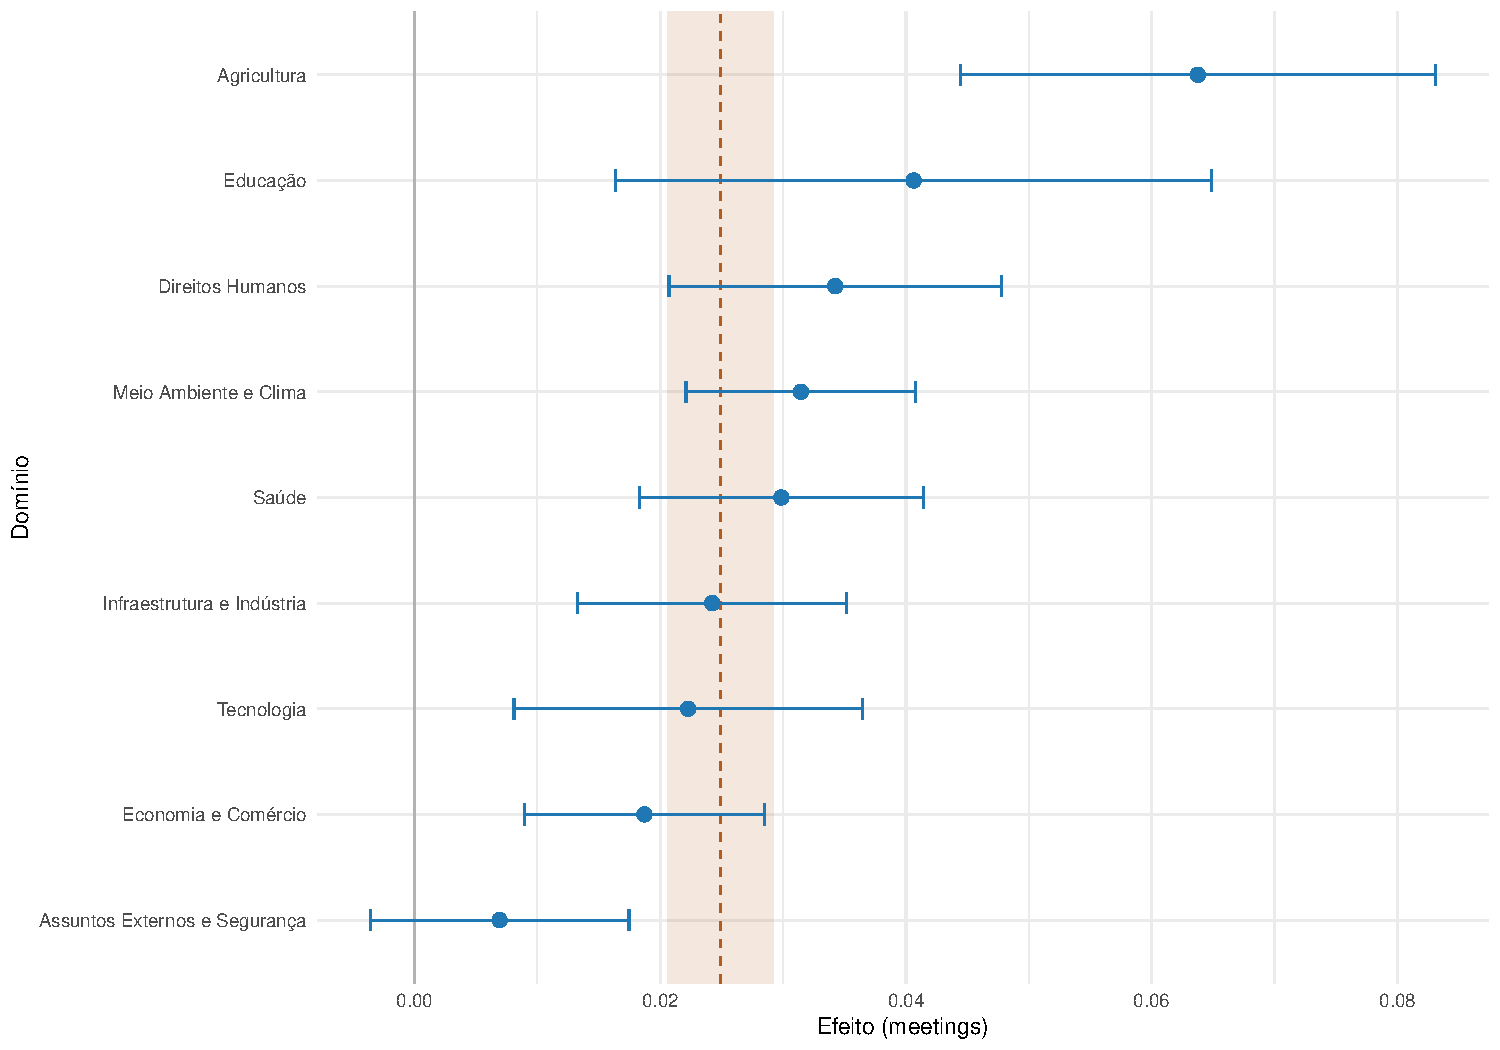
\includegraphics[width=\textwidth]{figures/fig_coeff_domains.pdf}
\caption{Efeito esperado \textit{ceteris paribus}: especificação linear (\acrshort{ppml}) para cada domínio}
\label{fig:effect_linear_ppml_domains}
\note{Cada ponto azul representa a estimativa do coeficiente associado a \textit{meetings} para um domínio específico de políticas públicas, refletindo o efeito marginal esperado de reuniões sobre o número de perguntas parlamentares naquele domínio, mantidos constantes os efeitos fixos. As linhas horizontais correspondem aos intervalos de confiança de 95\% para cada estimativa, indicando a incerteza estatística. A linha tracejada vermelha indica o efeito médio estimado para todos os domínios, servindo como referência para comparação entre áreas temáticas.}
\end{figure}

Além disso, os intervalos de confiança indicam que, apesar de variações na precisão das estimativas entre domínios, o sinal positivo do efeito é robusto e estatisticamente distinto de zero na maioria dos casos. Isso reforça a conclusão de que a associação entre intensidade de lobbying e atividade de fiscalização parlamentar não se restringe a um setor específico, mas se manifesta de forma generalizada no Parlamento Europeu, ainda que com intensidades distintas conforme o contexto temático.

De modo geral, esses resultados sugerem que o impacto do lobbying sobre a produção de perguntas parlamentares é um fenômeno transversal aos diferentes campos de políticas públicas, evidenciando a relevância desse mecanismo de influência em múltiplas agendas legislativas.


% \begin{figure}[htbp]
%     \centering
%     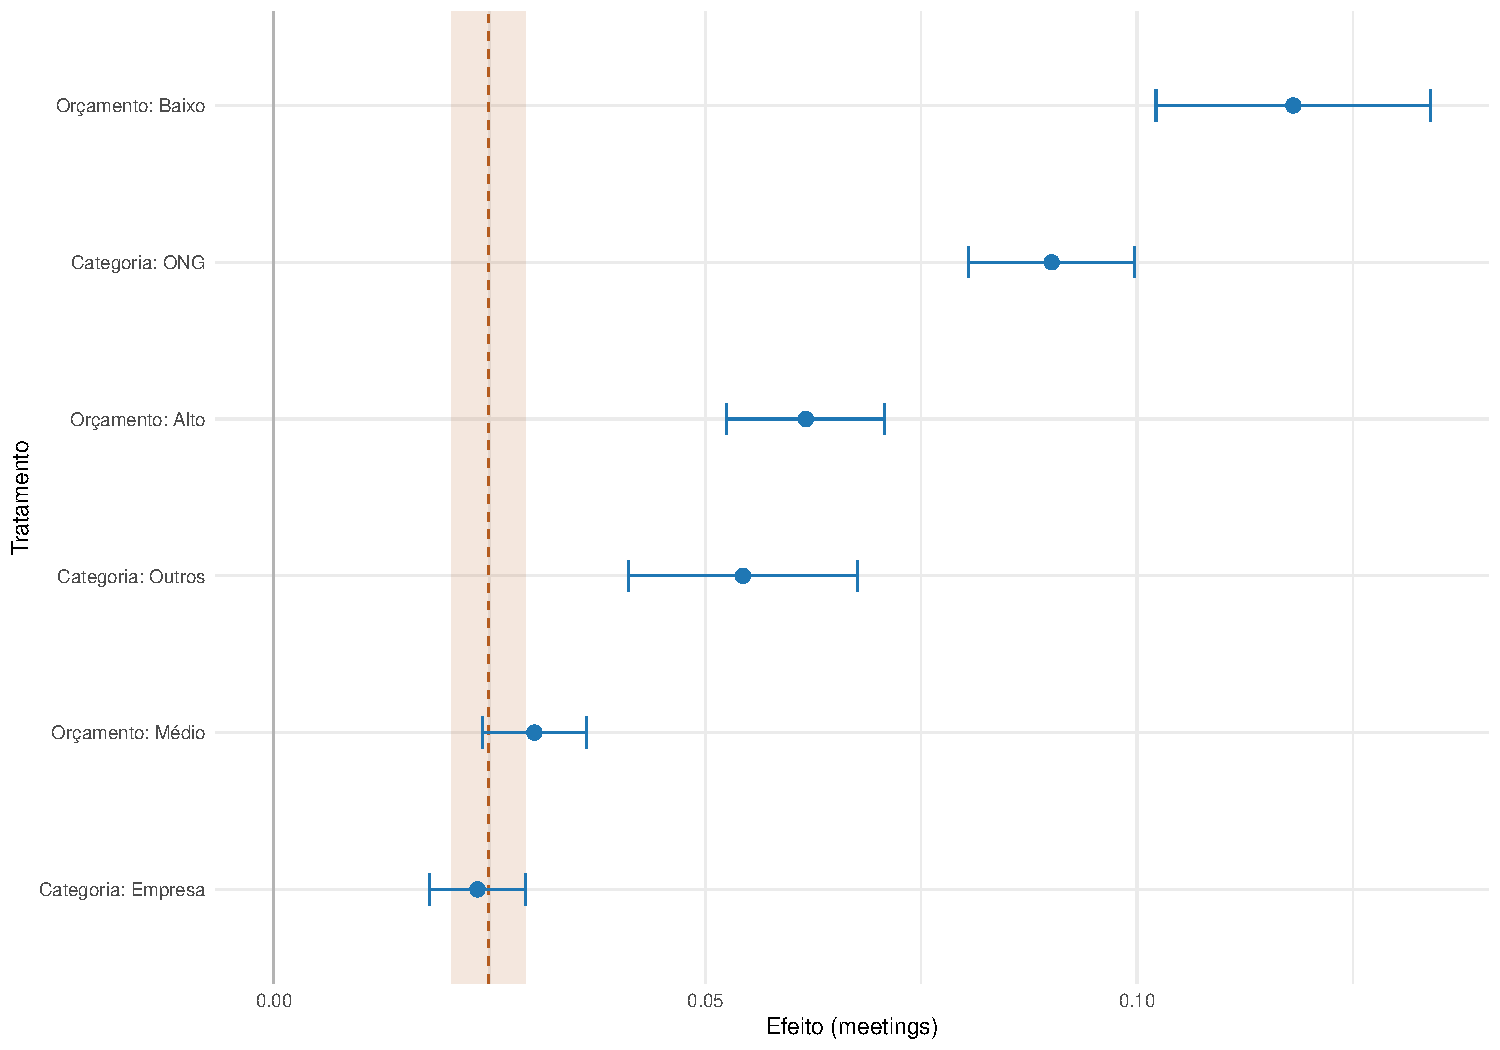
\includegraphics[width=\textwidth]{figures/fig_coeff_treatments_overall.pdf}
%     \caption{Efeito esperado \textit{ceteris paribus}: especificação linear (\acrshort{ppml}) para cada tratamento}
%     \label{fig:effect_linear_ppml_treatments}
%     \note{Cada ponto azul representa a estimativa do coeficiente associado a \textit{meetings} para um tratamento específico, refletindo o efeito marginal esperado de reuniões sobre o número de perguntas parlamentares, mantidos constantes os efeitos fixos. As linhas horizontais correspondem aos intervalos de confiança de 95\% para cada estimativa, indicando a incerteza estatística. A linha tracejada vermelha indica o efeito médio estimado para todos os tratamentos, servindo como referência para comparação entre tratamentos.}
% \end{figure}



\subsection{A Heterogeneidade do Efeito por Tipo de Ator}

A avaliação da Hipótese 2, que postula uma maior influência das empresas sobre a atividade parlamentar em comparação com outros atores, exige uma análise que transcenda a simples contagem de reuniões. Uma análise preliminar do efeito marginal por reunião, apresentada na Figura \ref{fig:effect_linear_ppml_treatments}, sugere que as \acrshort{ong}s, paradoxalmente, exercem uma influência maior por encontro. Este resultado, embora contraintuitivo, destaca a necessidade de um modelo mais completo que considere a heterogeneidade dos atores de lobby.

\begin{figure}[htbp]
    \centering
    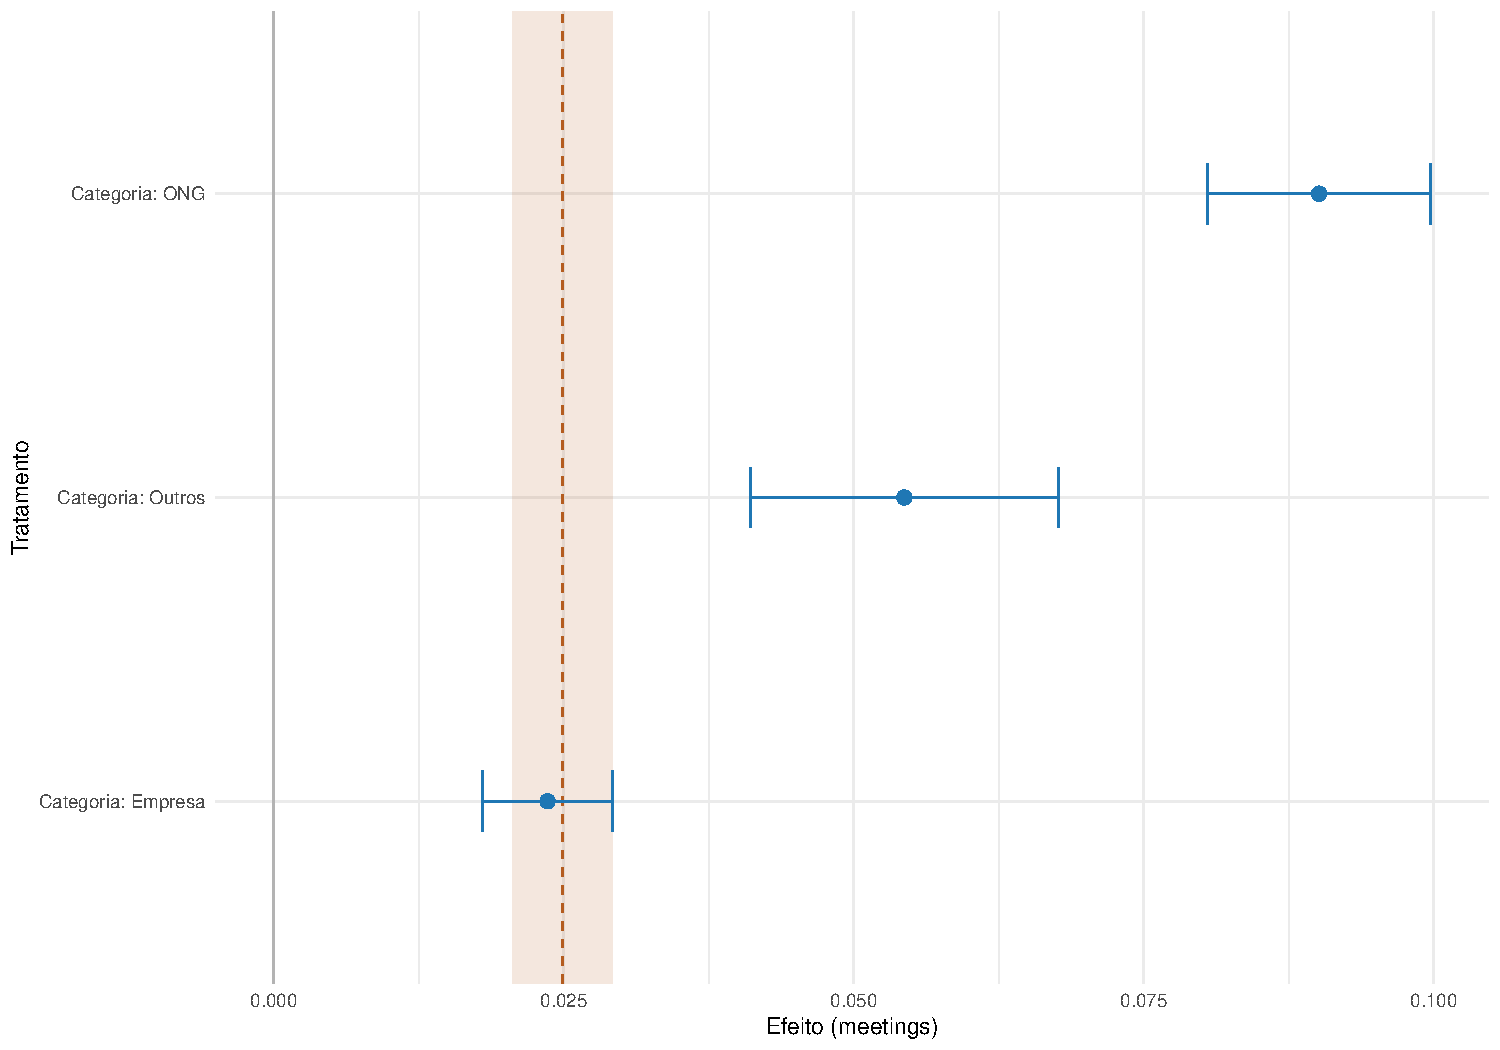
\includegraphics[width=\textwidth]{figures/h2_test/fig_coeff_treatments_overall.pdf}
    \caption{Efeito marginal por tipo de ator: especificação \acrshort{ppml}}
    \label{fig:effect_linear_ppml_treatments}
    \note{Cada ponto representa a estimativa do coeficiente para \textit{reuniões}, associado a um tipo de ator (tratamento), refletindo o efeito marginal esperado de uma única reunião sobre o número de perguntas parlamentares, mantendo os efeitos fixos constantes. As linhas horizontais indicam os intervalos de confiança de 95\%. A faixa vertical sombreada representa o intervalo de confiança do efeito médio geral, servindo como referência.}
\end{figure}

O efeito marginal isolado, contudo, é insuficiente para um teste robusto da hipótese. A influência total de um grupo de interesse não depende apenas da \textit{eficácia} de cada reunião, mas também da sua capacidade de assegurar \textit{acesso} -- isto é, o volume de reuniões que consegue realizar. Argumentamos que o impacto total é uma função dessas duas componentes: a frequência do acesso e a eficácia da persuasão em cada encontro.

Para capturar essa dualidade, adotamos uma estratégia de modelagem em duas etapas que decompõe o processo de lobby da seguinte forma:
\begin{itemize}
    \item \textbf{Acesso (Frequência):} O processo pelo qual um lobista garante reuniões com os \acrshort{mpe}s. Esta etapa, modelada com uma regressão Binomial Negativa, responde à pergunta: \textit{"Quantas reuniões um determinado lobista consegue obter?"}
    \item \textbf{Persuasão (Eficácia):} O processo pelo qual um lobista utiliza uma reunião para influenciar a atividade de um \acrshort{mpe}. Esta etapa, modelada com \acrshort{ppml}, responde à pergunta: \textit{"Quão eficaz é uma única reunião para gerar atividade parlamentar?"}
\end{itemize}

Esta abordagem permite-nos decompor e compreender os mecanismos através dos quais diferentes atores exercem influência.

Para estimar o volume de reuniões (Acesso) - Etapa 1 -, utilizamos um modelo de regressão Binomial Negativo, apropriado para dados de contagem com sobredispersão. A variável dependente é o número de reuniões que um lobista realiza, e as variáveis explicativas incluem o orçamento de lobby, a categoria do ator (\acrshort{ong}, Empresa, Outros) e um termo de interação entre orçamento e categoria, além de controles setoriais e geográficos.

O coeficiente de interação entre ser uma empresa e o orçamento de lobby é particularmente revelador. Um resultado positivo e estatisticamente significativo para este termo indica que as empresas não só tendem a realizar mais reuniões em média, mas também demonstram uma "eficiência alocativa" superior: cada aumento percentual no seu orçamento se traduz num aumento maior no número de reuniões em comparação com as \acrshort{ong}s. A Figura \ref{fig:h2_pred_meetings} ilustra essa dinâmica, mostrando o número esperado de reuniões em função do orçamento.

\begin{figure}[htbp]
    \centering
    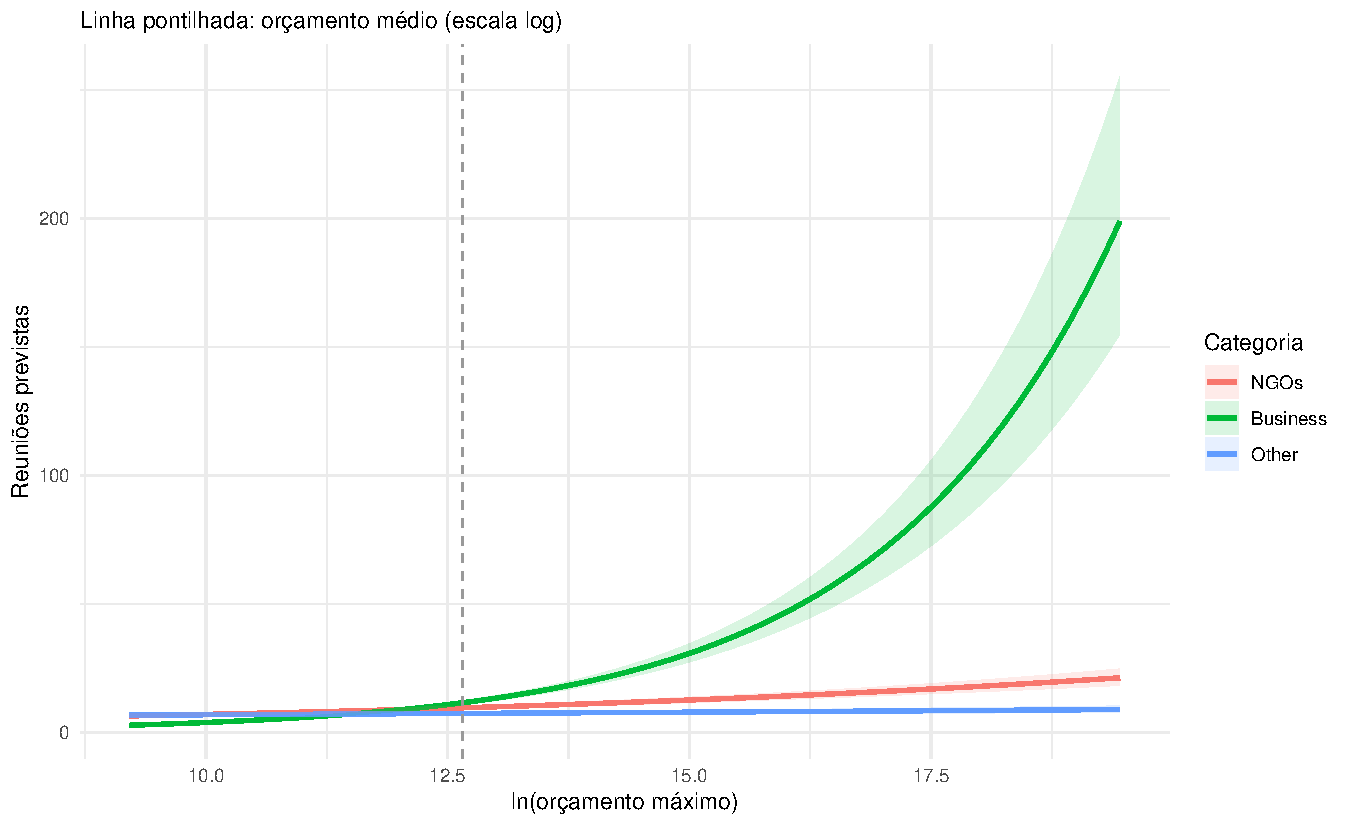
\includegraphics[width=\textwidth]{figures/h2_test/fig_pred_meetings_vs_budget_centered_by_category.pdf}
    \caption{Previsão do número de reuniões por categoria e orçamento}
    \label{fig:h2_pred_meetings}
    \note{O gráfico exibe o número esperado de reuniões (eixo Y) em função do logaritmo do orçamento de lobby (eixo X), com base no modelo Binomial Negativo. As curvas representam a previsão para cada categoria de ator, mantendo as demais variáveis em seus valores médios ou modais. A linha tracejada vertical indica o orçamento médio na amostra. As áreas sombreadas correspondem aos intervalos de confiança de 95\%.}
\end{figure}

Observa-se um ponto de inflexão: abaixo de um orçamento de aproximadamente \$27.000 ($\approx e^{10.2}$), as \acrshort{ong}s tendem a realizar mais reuniões. Acima desse limiar, a capacidade das empresas de converter recursos financeiros em acesso torna-se proeminente, e a disparidade cresce exponencialmente com o orçamento.

Para estimar o efeito agregado (Etapa 2), combinamos os resultados das duas etapas, multiplicando o número esperado de reuniões (o \textit{Acesso}, da Etapa 1) pelo efeito marginal por reunião (a \textit{Persuasão}, da Figura \ref{fig:effect_linear_ppml_treatments}) para cada categoria de ator e nível de orçamento. O resultado, ilustrado na Figura \ref{fig:h2_total_effects}, representa uma aproximação de primeira ordem do impacto total do lobby.

\begin{figure}[htbp]
    \centering
    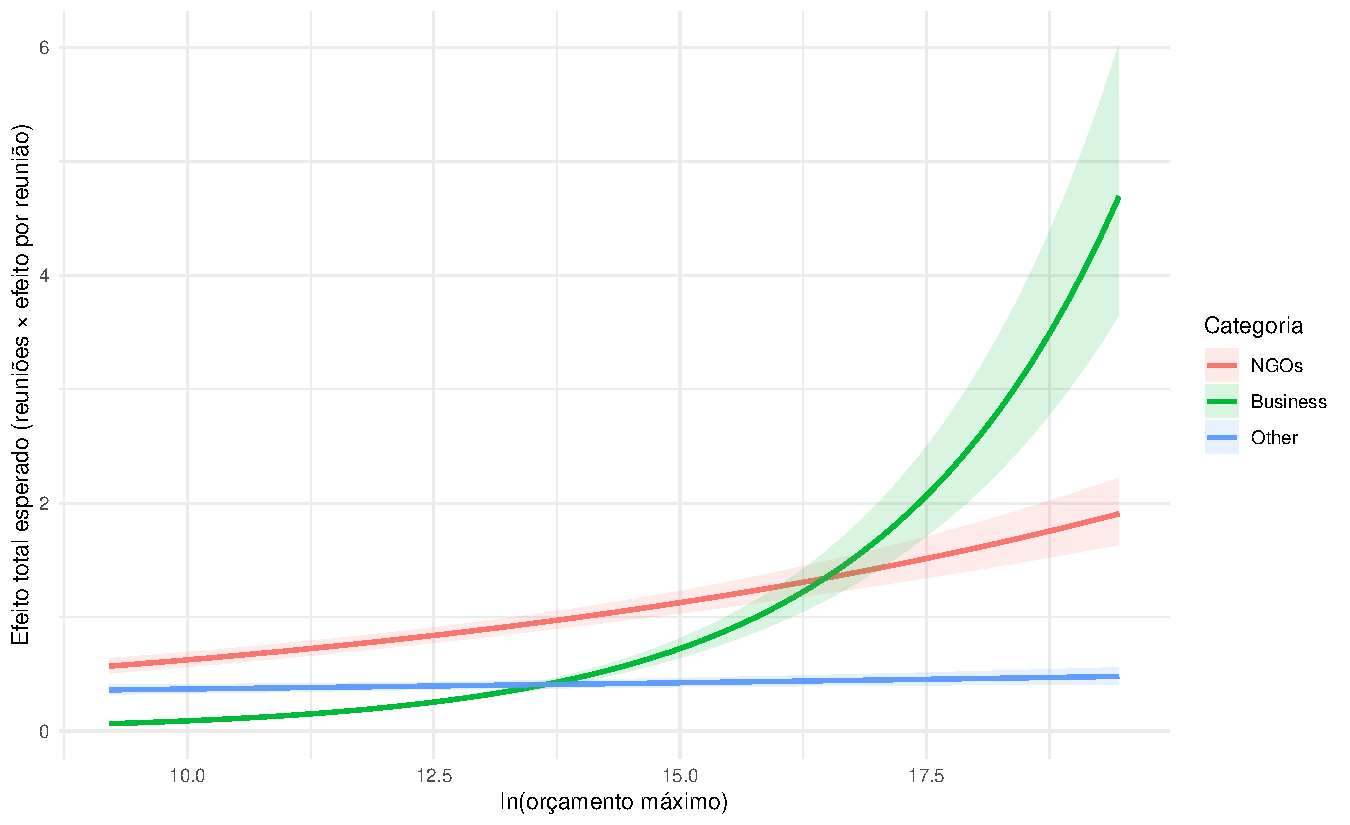
\includegraphics[width=\textwidth]{figures/h2_test/fig_total_effect_vs_budget_by_category.pdf}
    \caption{Efeito total estimado por categoria e orçamento}
    \label{fig:h2_total_effects}
    \note{O gráfico representa o efeito total esperado, calculado como o produto do número previsto de reuniões (da Figura \ref{fig:h2_pred_meetings}) e do coeficiente de efeito marginal por reunião (da Figura \ref{fig:effect_linear_ppml_treatments}). O eixo Y representa o aumento esperado no número de perguntas parlamentares.}
\end{figure}

A análise do efeito total revela uma relação complexa e não-linear. Embora uma única reunião com uma \acrshort{ong} seja, em média, mais influente, a superioridade das empresas em garantir um grande volume de acesso, especialmente quando dispõem de orçamentos elevados, reverte essa vantagem. Para orçamentos abaixo de \$8,8 milhões ($\approx e^{16}$), o efeito total das \acrshort{ong}s permanece superior. No entanto, acima de \$40 milhões ($\approx e^{17.5}$), o efeito agregado das empresas torna-se substancialmente maior.

Estes resultados oferecem um suporte nuançado à Hipótese 2 e dialogam diretamente com a literatura sobre os mecanismos de influência do lobby. A influência das empresas não é incondicionalmente superior, mas torna-se dominante quando alavancada por vastos recursos financeiros, um achado que se alinha com a discussão sobre a desigualdade de representação \cite{mahoney_lobbying_2007}. A decomposição do efeito em "acesso" e "persuasão" permite-nos explorar as diferentes naturezas dos recursos mobilizados pelos atores, conforme aponta a literatura \cite{de_figueiredo_advancing_2014, Pop2013Lobbying}.

A maior eficácia marginal por reunião das \acrshort{ong}s pode ser interpretada à luz do seu capital reputacional e da sua legitimidade percebida \cite{bunea2018legitimacy}. Do ponto de vista do comportamento parlamentar, interagir com \acrshort{ong}s pode ser uma estratégia de \textit{vote-seeking} para os \acrshort{mpe}s, que buscam sinalizar alinhamento com causas de interesse público e, assim, aumentar seu apelo eleitoral \cite{Ibenskas2021, mayhew2004congress}.

Por outro lado, a capacidade das grandes corporações de converter recursos financeiros em um volume massivo de acesso aponta para outro mecanismo de influência: a subsidiação de informação. Para atingir seus objetivos de carreira (\textit{career-seeking}) e de formulação de políticas (\textit{policy-seeking}), os parlamentares necessitam de informação técnica e especializada \cite{daniel2015career, kluver_informational_2012}. As grandes empresas, com seus recursos, estão em posição privilegiada para fornecer este subsídio informacional, estabelecendo uma relação de troca \cite{huwyler_no_2023} que lhes garante um acesso privilegiado e contínuo. Assim, a capacidade de "saturar" o ambiente informacional com interações frequentes parece ser um fator decisivo para a sua influência agregada.

É importante notar que esta abordagem metodológica assenta na premissa de \textit{separabilidade} entre os processos de "acesso" e "persuasão". Esta premissa implica que, após controlarmos pelas variáveis observáveis (como o orçamento), os fatores não observados que tornam um lobista eficaz em garantir reuniões são estatisticamente independentes dos fatores não observados que o tornam influente durante essas reuniões. A suposição de separabilidade poderia ser violada se, por exemplo, uma "qualidade" ou "reputação" intrínseca do lobista, não capturada pelo modelo, afetasse simultaneamente a sua capacidade de agendar reuniões e a recetividade dos parlamentares às suas propostas. Nesse cenário, a multiplicação dos efeitos poderia levar a uma estimativa enviesada do impacto total.

Em suma, os resultados indicam que, embora o discurso das \acrshort{ong}s possa ter maior ressonância por interação, a capacidade financeira das grandes empresas permite-lhes superar essa desvantagem através de uma presença quantitativamente esmagadora, confirmando a importância crítica dos recursos na determinação da influência política.
\subsubsection{Teste da hipótese 3: O Efeito do Lobby em Temas Salientes}

A Hipótese 3 postula que, em temas de maior saliência, o lobby exercido por organizações não empresariais (como as \acrshort{ong}s) tem uma maior probabilidade de influenciar a atividade legislativa dos \acrshort{mpe}s em comparação com o lobby de organizações empresariais. A lógica subjacente é que, quando um tema está sob intenso escrutínio público, os parlamentares se tornam mais sensíveis a argumentos que ressoam com a opinião pública e a interesses difusos, frequentemente representados por \acrshort{ong}s.

Para testar esta hipótese, mantivemos a estrutura do modelo \acrshort{ppml} com efeitos fixos, garantindo a consistência com as análises anteriores. A principal diferença metodológica foi a introdução de uma variável para capturar a saliência de um tema e a sua interação com os diferentes tipos de lobistas.

A saliência foi operacionalizada como uma proxy baseada na intensidade da atividade de lobby, uma abordagem que encontra respaldo na literatura \cite{baumgartner2010agendas}. Especificamente, criamos uma variável (salience\_std) que mede o volume total de reuniões de lobby dentro de cada domínio temático para cada período mensal, padronizada para ter média zero e desvio padrão um. Um valor mais alto nesta variável indica que um tema atraiu mais atenção de todos os grupos de interesse, sendo, portanto, considerado mais saliente.

O modelo econométrico foi então especificado para incluir termos de interação entre cada categoria de lobista (Empresa, \acrshort{ong}, Outros) e a variável de saliência, apresentado na Equação \ref{eq:modelo_h3}. Esta especificação permite-nos estimar como o efeito marginal de uma reunião de cada tipo de ator varia em função do nível de saliência do tema. Os resultados da regressão estão sumarizados na Tabela \ref{tab:h3_interaction} e visualizados no gráfico de efeitos marginais na Figura \ref{fig:h3_marginal_effects}.

\begin{table}
\centering
\begin{talltblr}[         %% tabularray outer open
entry=none,label=none,
note{}={+ p \num{< 0.1}, * p \num{< 0.05}, ** p \num{< 0.01}, *** p \num{< 0.001}},
]                     %% tabularray outer close
{                     %% tabularray inner open
colspec={Q[]Q[]},
column{2}={}{halign=c,},
column{1}={}{halign=l,},
hline{10}={1-2}{solid, black, 0.05em},
}                     %% tabularray inner close
\toprule
& PPML com Interação (H3) \\ \midrule %% TinyTableHeader
Empresa (base) & \num{0.035}*** \\
& (\num{0.006}) \\
ONG (base) & \num{0.090}*** \\
& (\num{0.006}) \\
Outros (base) & \num{0.032}** \\
& (\num{0.010}) \\
Empresa x Saliência & \num{-0.022}*** \\
& (\num{0.005}) \\
Num.Obs. & \num{600237} \\
R2 & \num{0.253} \\
RMSE & \num{0.56} \\
Std.Errors & by: cl\_dt \\
FE: fe\_ct & X \\
FE: fe\_pt & X \\
FE: fe\_dt & X \\
\bottomrule
\end{talltblr}
\end{table}



\begin{figure}[htbp]
    \centering
    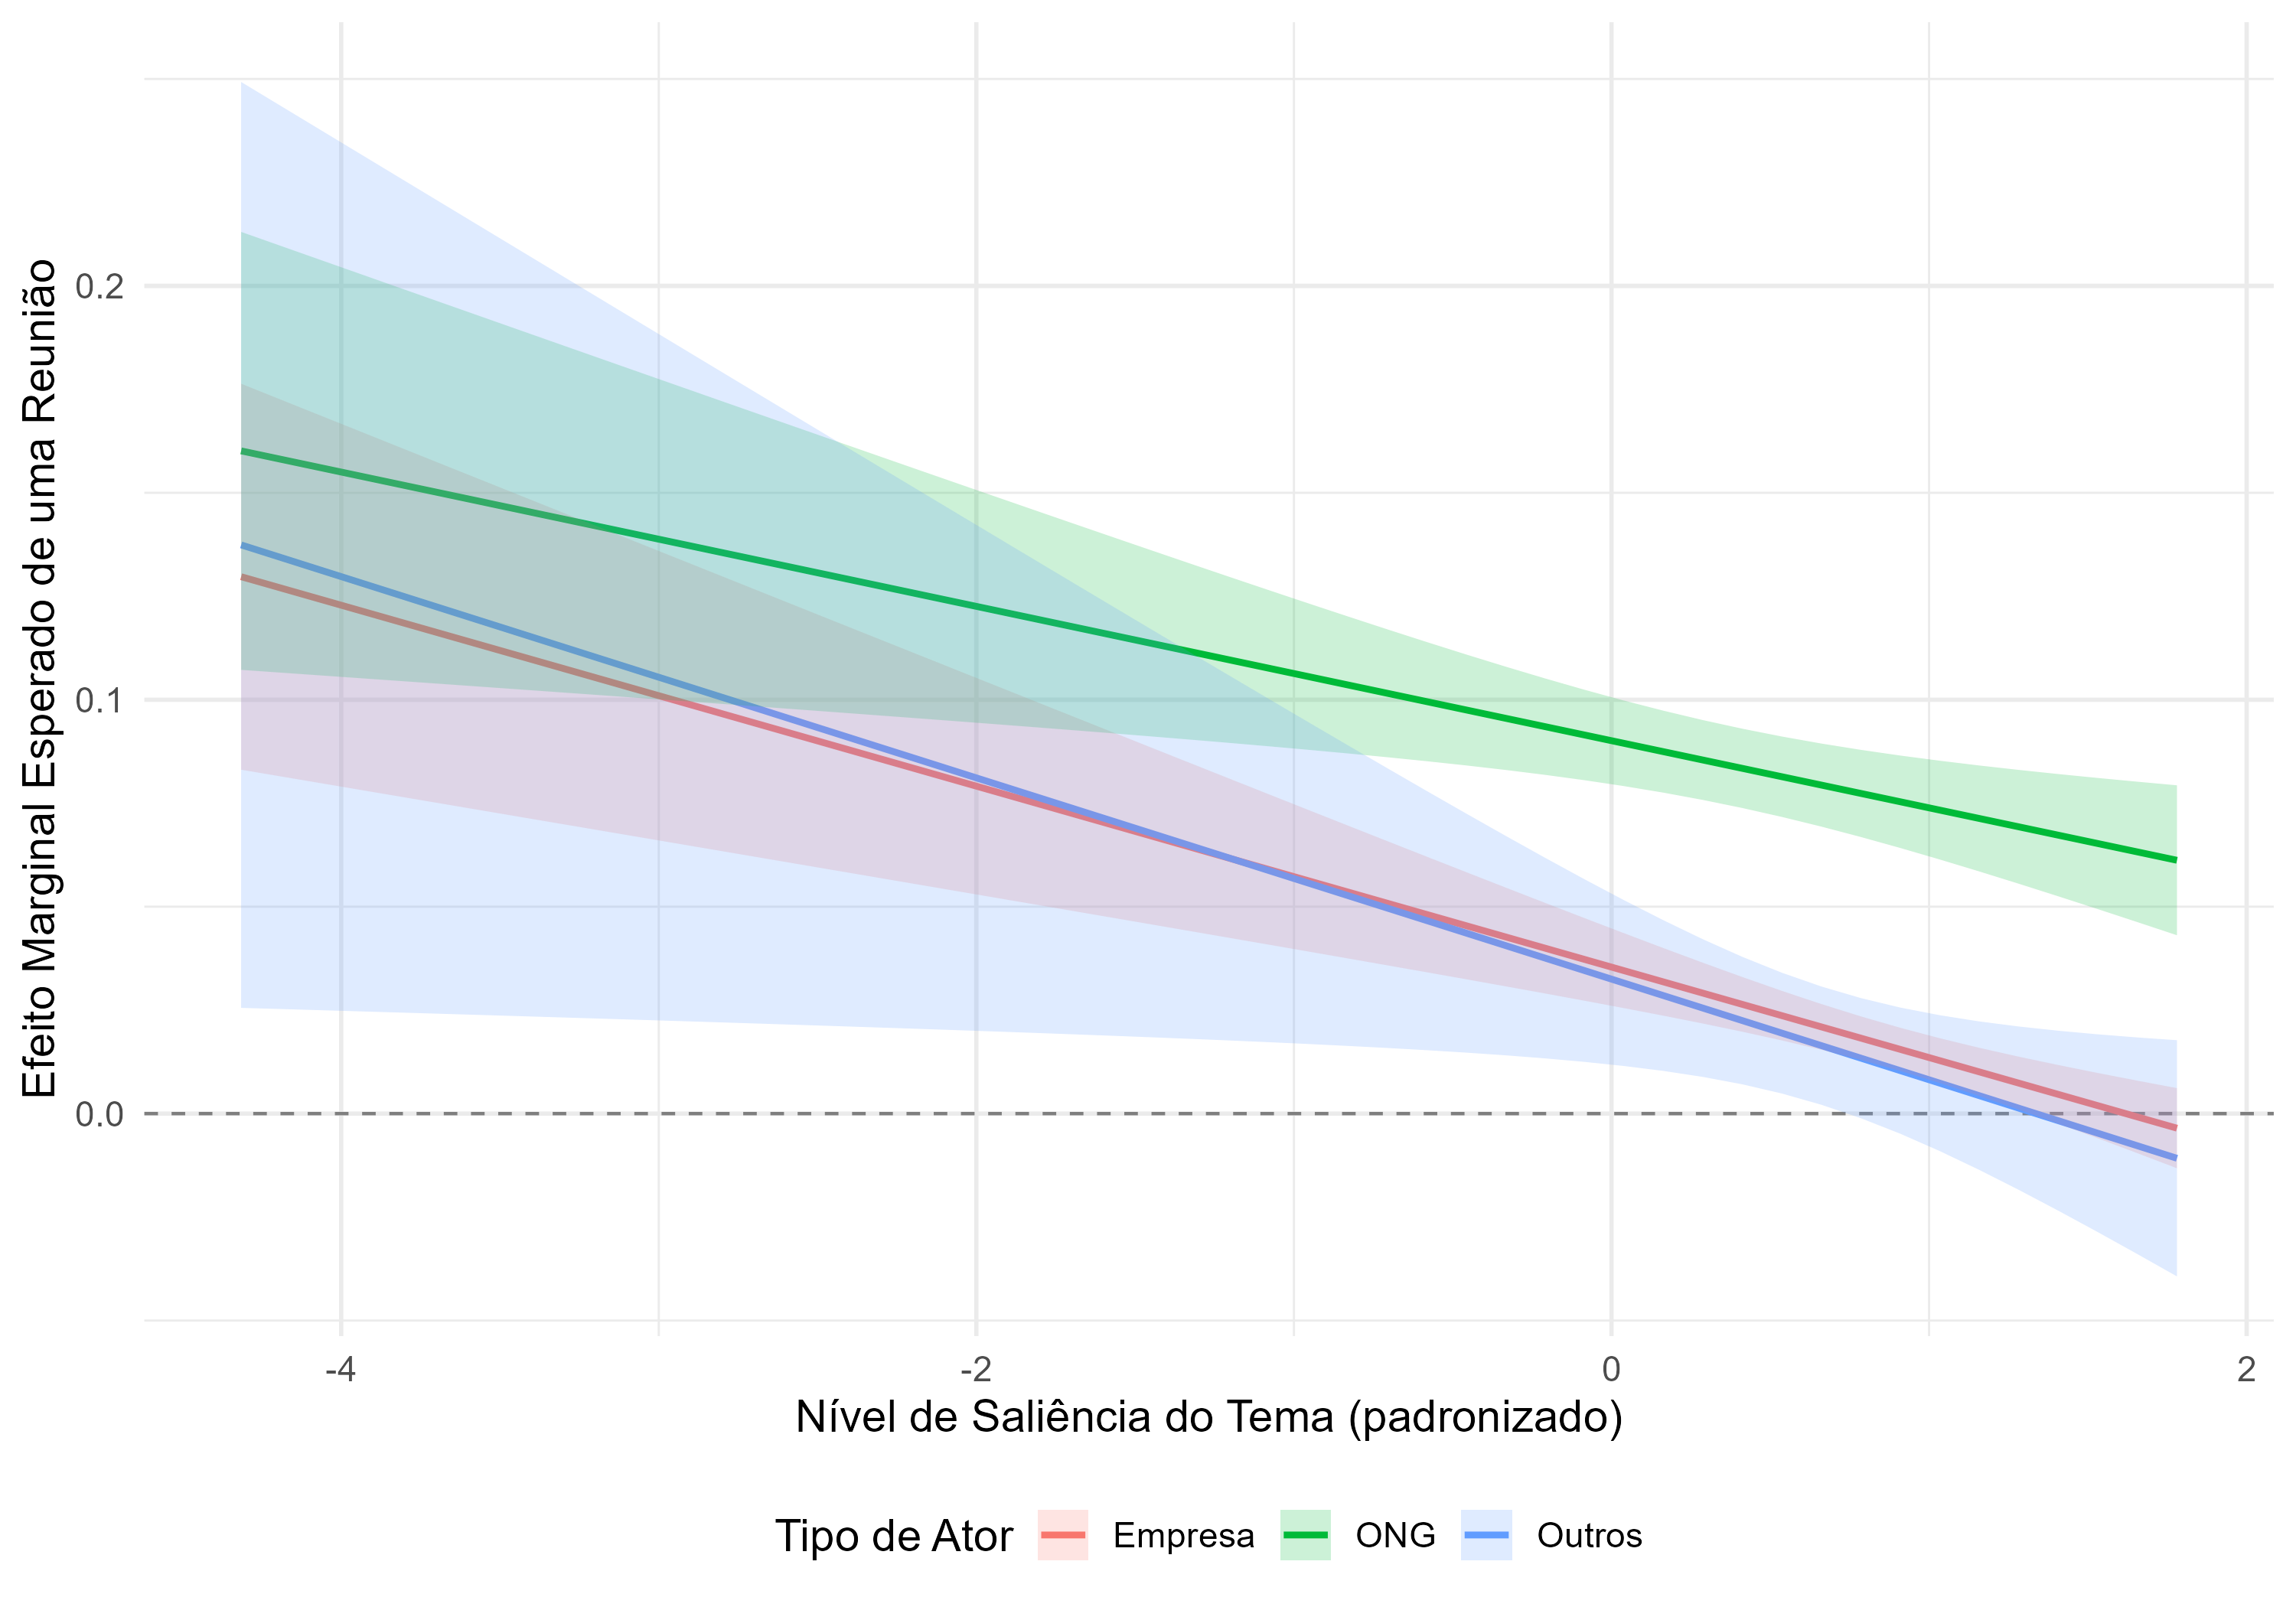
\includegraphics[width=\textwidth]{figures/h3_test/fig_h3_marginal_effects_manual.png}
    \caption{Efeito do Lobby Condicional à Saliência do Tema}
    \label{fig:h3_marginal_effects}
    \note{O gráfico exibe o efeito marginal esperado de uma única reunião sobre o número de perguntas parlamentares (eixo Y) em diferentes níveis de saliência do tema (eixo X). As linhas representam a estimativa para cada categoria de ator, e as áreas sombreadas correspondem aos intervalos de confiança de 95\%, calculados via bootstrap.}
\end{figure}

A análise revela um padrão complexo que contradiz parcialmente, mas também enriquece, a Hipótese 3. Contrariamente à expectativa de que o efeito das \acrshort{ong}s aumentaria com a saliência, observamos que o efeito marginal de uma reunião \textbf{diminui} para todos os grupos à medida que um tema se torna mais saliente (coeficiente negativo para todos os grupos nas variáveis de interação). Este achado está em forte alinhamento com a literatura, que sugere que a influência do lobby direto decresce quando a opinião pública e a atenção da mídia se intensificam, forçando os parlamentares a se alinharem a considerações eleitorais mais amplas \cite{mahoney_lobbying_2007, kollman1998outside}.

No entanto, a análise revela uma heterogeneidade crucial na taxa dessa diminuição. Três pontos principais se destacam na Figura \ref{fig:h3_marginal_effects}. Em temas de baixa saliência (à esquerda do gráfico), o efeito das \acrshort{ong}s é similar estatisticamente ao de empresas e outros atores. Isso pode ser observado pela intersecção das áreas sombreadas das linhas, que indicam o intervalo de confiança de 95\% das estimativas.
    
À medida que a saliência aumenta (movendo-se para a direita no gráfico), a vantagem comparativa das \acrshort{ong}s se acentua significativamente. O efeito do lobby de empresas e de outros atores decai rapidamente, enquanto o efeito das \acrshort{ong}s se mostra muito mais resiliente, diminuindo a uma taxa consideravelmente menor.
    
Em temas de alta saliência, onde a influência de empresas e outros grupos se torna estatisticamente indistinguível de zero (seus intervalos de confiança cruzam a linha pontilhada), o efeito das \acrshort{ong}s permanece positivo, robusto e estatisticamente significativo. É precisamente neste contexto de maior escrutínio público que a sua influência relativa se torna mais pronunciada.

Os resultados validam a Hipótese 3. Em temas de maior saliência, o lobby de organizações não empresariais é, de fato, mais eficaz em aumentar a atividade parlamentar em comparação com o lobby empresarial. A nuance importante é que essa maior eficácia não se manifesta como um aumento absoluto do efeito, mas sim como uma resiliência superior à pressão do escrutínio público, o que amplia a sua vantagem comparativa.

Esta descoberta dialoga diretamente com a teoria sobre os recursos do lobby e os incentivos parlamentares. Em temas de baixa saliência, os parlamentares, focados em seus objetivos de formulação de políticas (\textit{policy-seeking}), podem valorizar o subsídio informacional técnico fornecido por empresas. Contudo, quando um tema ganha visibilidade, os incentivos de reeleição (\textit{vote-seeking}) tornam-se dominantes \cite{mayhew2004congress}. Nesse contexto, alinhar-se a interesses empresariais pode ter um custo político elevado, enquanto responder a \acrshort{ong}s, que detêm maior capital de legitimidade \cite{bunea2018legitimacy}, reforça a imagem pública do parlamentar.

Os achados confirmam que a influência do lobby é altamente contextual e que, sob o escrutínio público, a vantagem se desloca para os atores percebidos como representantes de interesses mais amplos e difusos.

        \chapter{Resultados}
\label{chapter:resultados}
Este capítulo tem como objetivo apresentar e discutir os principais resultados empíricos da tese, respondendo às hipóteses formuladas e avaliando o impacto do lobby sobre a atividade legislativa no Parlamento Europeu. Inicialmente, são descritas as características dos lobistas e dos parlamentares presentes na amostra, bem como padrões descritivos das reuniões e perguntas parlamentares. Em seguida, são apresentados os resultados dos testes das hipóteses centrais, com análise dos efeitos estimados, heterogeneidades e mecanismos identificados. Por fim, o capítulo discute as implicações dos achados para o debate sobre influência política e transparência institucional.

\section{Lobby no Parlamento: atores, recursos e agendas}
\label{sec:resultados_descritica_lobistas}
A Tabela \ref{tab:dist_orgs_reunioes} apresenta a distribuição de lobistas e sua atividade (mensurada pelo número de reuniões) por categoria organizacional. Os dados revelam uma predominância de interesses empresariais, que constituem o maior grupo tanto em número de organizações (2.409) quanto em volume de reuniões (22.427). Em média, cada organização empresarial realizou 9,31 reuniões, a maior taxa entre as categorias. As ONGs figuram como o segundo grupo mais ativo, seguidas pela categoria "Outros".

\begin{table}[!htbp]
\centering
\caption{Distribuição de organizações, reuniões e reuniões por lobista, por categoria de organização}
\label{tab:dist_orgs_reunioes}
\begin{tabular}{lccc}
\hline
Categoria & Organizações & Reuniões & Reuniões por Organização \\
\hline
Empresarial & 2.409 & 22.427 & 9,31 \\
ONGs & 1.271 & 10.966 & 8,63 \\
Outros & 1.042 & 6.950 & 6,67 \\
\hline
Total & 4.722 & 40.343 & 8,54 \\
\hline  
\end{tabular}
\end{table}

Esses resultados corroboram uma vasta literatura que aponta para a assimetria de recursos e representação no universo do lobby. Interesses empresariais, que dispõem de maiores recursos financeiros, tendem a predominar na atividade de lobby \cite{de_figueiredo_advancing_2014}. No contexto específico da União Europeia, estudos demonstram que grupos empresariais e associações nacionais são os mais presentes \cite{dur20212wholobbies, eising2007institutional}, o que levou alguns autores a caracterizarem o sistema como um "pluralismo de elite" \cite{coen1997evolution, schmidt2006procedural}.

A intensidade da atividade, refletida no elevado número total de reuniões (40.343), sinaliza uma forte competição pelo acesso aos tomadores de decisão, um recurso considerado escasso pela literatura \cite{hall1990buying}. Embora os atores empresariais detenham mais acesso, a presença expressiva de ONGs indica um ambiente competitivo, e não monolítico. Essa coexistência sugere que diferentes tipos de organizações mobilizam recursos distintos para influenciar o processo político. Enquanto interesses empresariais podem alavancar recursos financeiros e expertise técnica, ONGs e outros grupos da sociedade civil podem recorrer a recursos como legitimidade, representatividade e apoio público para defender suas causas \cite{Coen2019, dur_measuring_2008}.

Portanto, a análise descritiva inicial já delineia uma das tensões centrais investigadas neste trabalho: o desequilíbrio de poder e recursos entre interesses empresariais e outros setores da sociedade, e como essa assimetria se manifesta na competição por influência política no \acrshort{pe}.


% Análise do orçamento máximo declarado
A análise do orçamento máximo declarado por categoria (Figura \ref{fig:budget_ln_boxplot}), em escala logarítmica, revela padrões distributivos distintos. O grupo empresarial, embora mais numeroso em quantidade de organizações, exibe a menor mediana de orçamento e uma distribuição notavelmente mais concentrada, o que sugere uma maior homogeneidade nos gastos com lobby declarados por essas entidades.

Em contrapartida, as ONGs e a categoria "Outros" apresentam medianas mais elevadas e uma variância substancialmente maior. Essa dispersão indica uma forte heterogeneidade interna, sugerindo a coexistência de organizações com recursos modestos e outras com orçamentos muito elevados, que influenciam a distribuição.

\begin{figure}[!htbp]
\centering
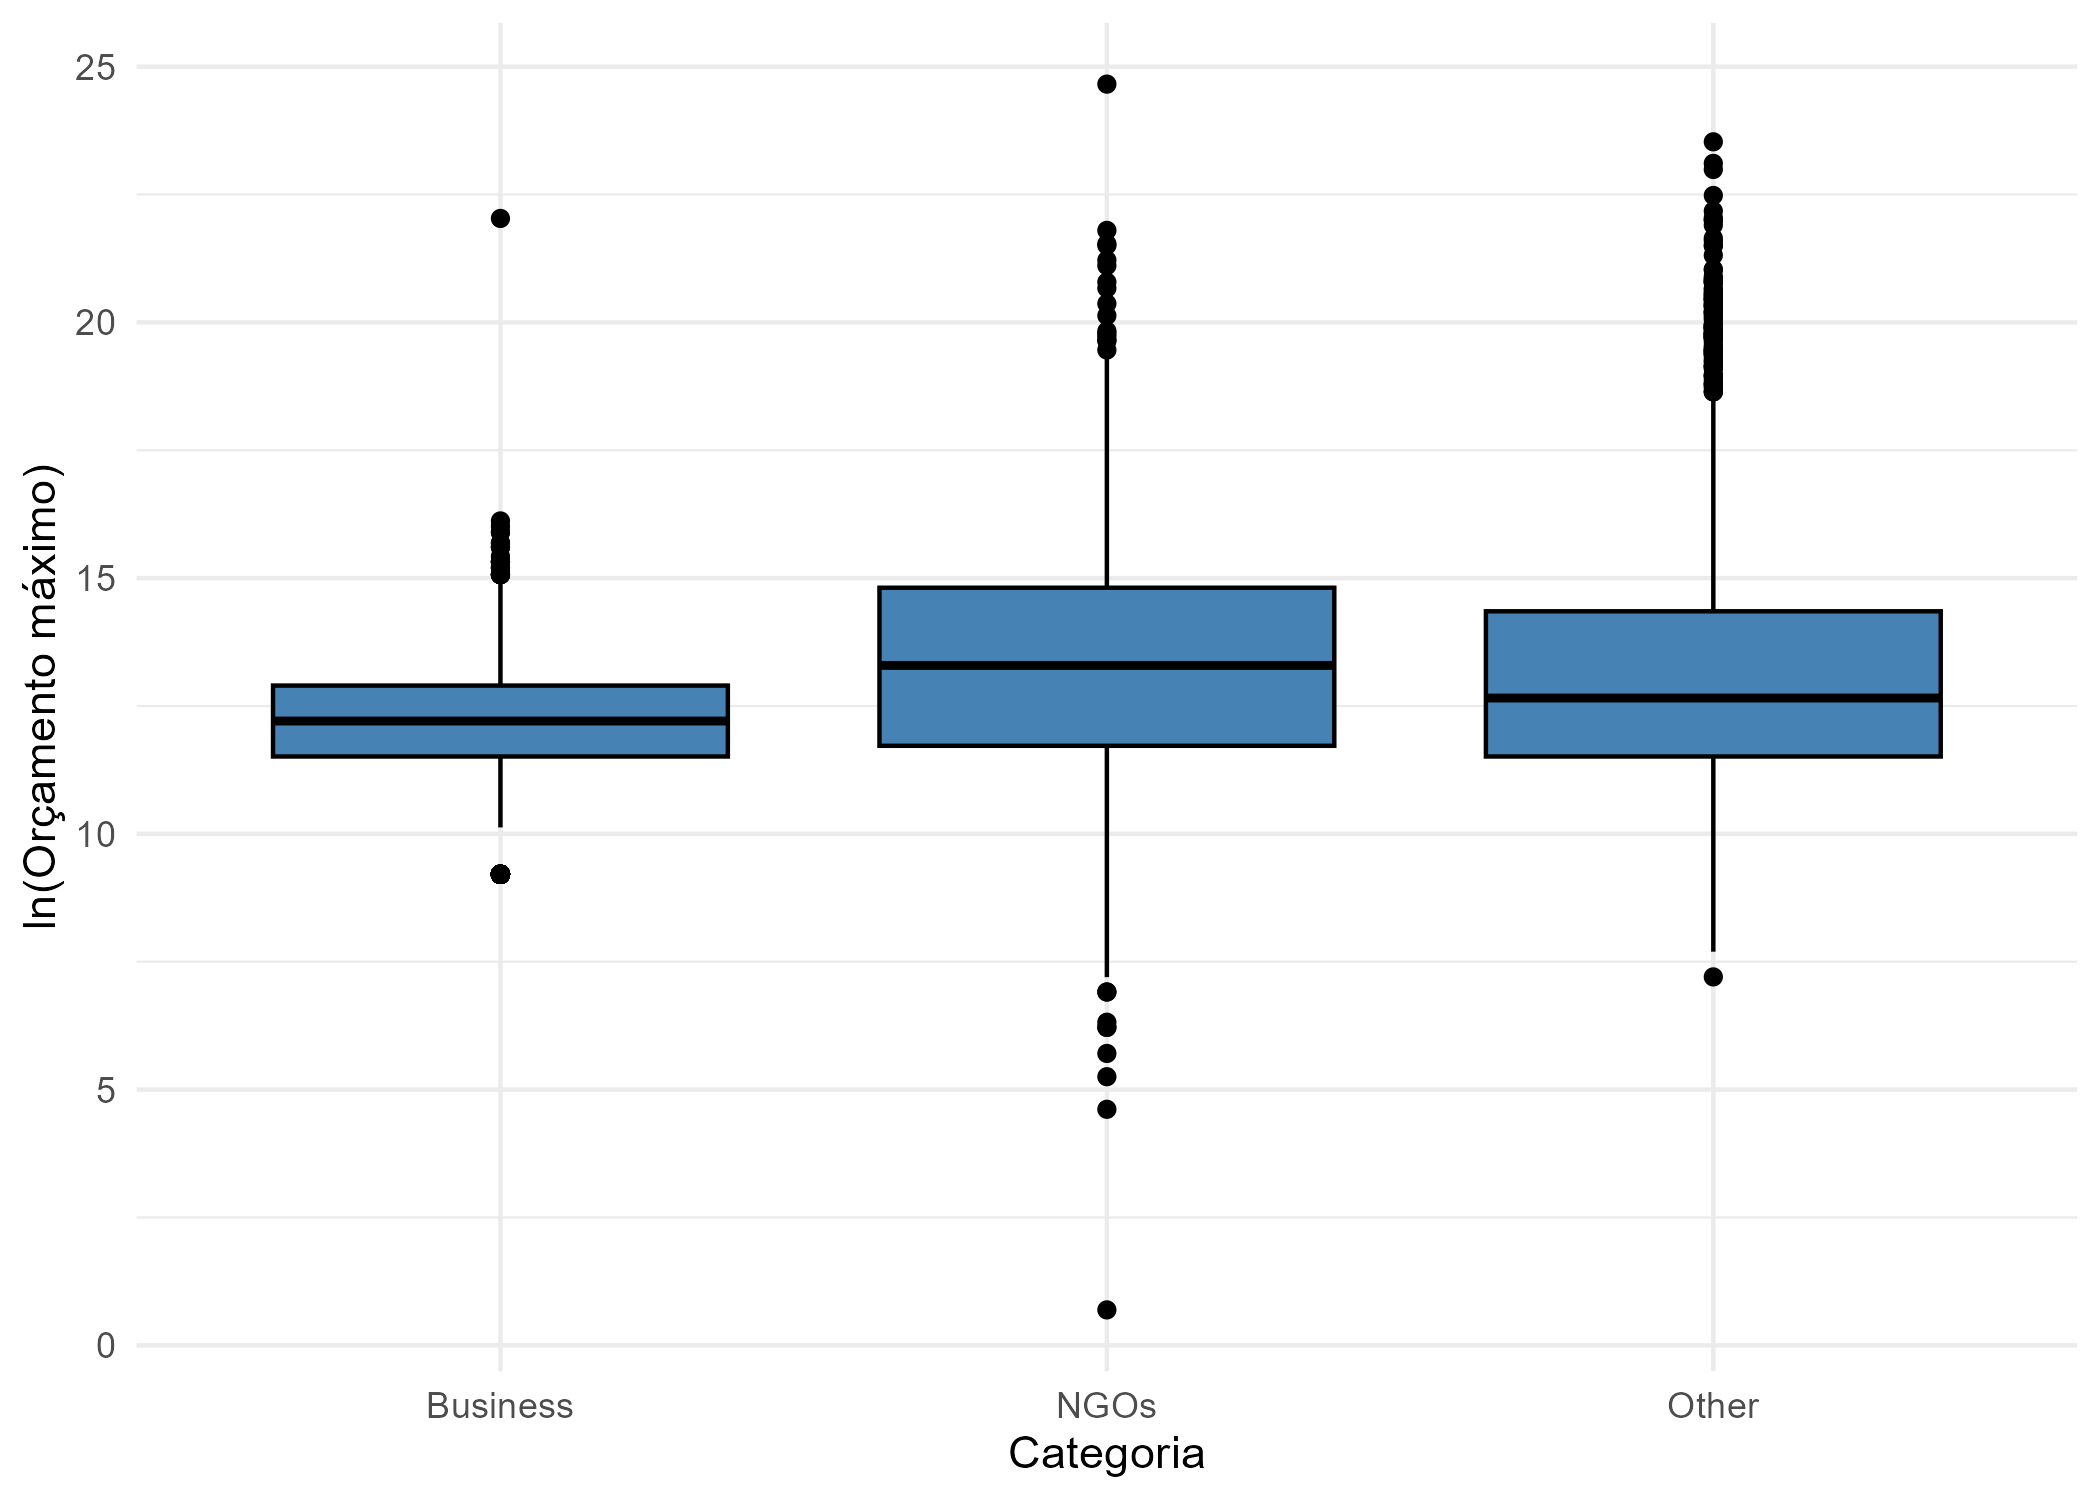
\includegraphics[width=0.75\textwidth]{figures/descriptives_lobbyists/boxplot_max_budget_by_category.png}
\caption{Distribuição de orçamento máximo declarado (\textit{ln(Orçamento Máximo Declarado)}) por categoria}
\label{fig:budget_ln_boxplot}
\end{figure}

Este achado é particularmente interessante, pois parece tensionar a premissa da literatura de que interesses empresariais dominam em termos de recursos financeiros \cite{de_figueiredo_advancing_2014, dur20212wholobbies}. Uma interpretação possível é que a categoria empresarial seja composta por um grande número de atores com gastos mais padronizados, enquanto as categorias de ONGs e "Outros" contêm algumas organizações muito grandes, cujos orçamentos massivos podem refletir campanhas de alto custo ou estruturas de financiamento distintas. A alta variância pode, ainda, ser um reflexo de diferentes estratégias: enquanto empresas podem ter um dispêndio mais constante, ONGs podem mobilizar grandes somas para temas de alta saliência, onde a opinião pública é um fator crucial \cite{mahoney_lobbying_2007}.

Adicionalmente, a concentração no grupo empresarial pode estar relacionada ao problema da ação coletiva \cite{olson1971logic}, onde muitas empresas optam por atuar por meio de associações — que podem estar classificadas na categoria "Outros". De todo modo, os dados reforçam que a relação entre recursos financeiros e influência não é direta \cite{simon_notes_1953}, e que a capacidade de mobilizar diferentes tipos de recursos — não apenas financeiros, mas também de legitimidade e informação \cite{Coen2019} — é central para a dinâmica do lobby na \acrshort{ue}.


% Distribuição geográfica
A análise da distribuição geográfica dos lobistas (Figura \ref{fig:country_distribution}) revela uma acentuada concentração em polos institucionais da União Europeia, com Bélgica (24,2\%), Alemanha (15,3\%) e França (10,1\%) abrigando a maioria das organizações. Este padrão corrobora a tese da vantagem da proximidade institucional: a presença massiva na Bélgica, sede da Comissão Europeia e de grande parte das atividades do Parlamento, e na França, que sedia as sessões plenárias do Parlamento em Estrasburgo, é uma resposta estratégica à complexa governança multinível da \acrshort{ue} \cite{richardson2000government}.

\begin{figure}[!htbp]
\centering
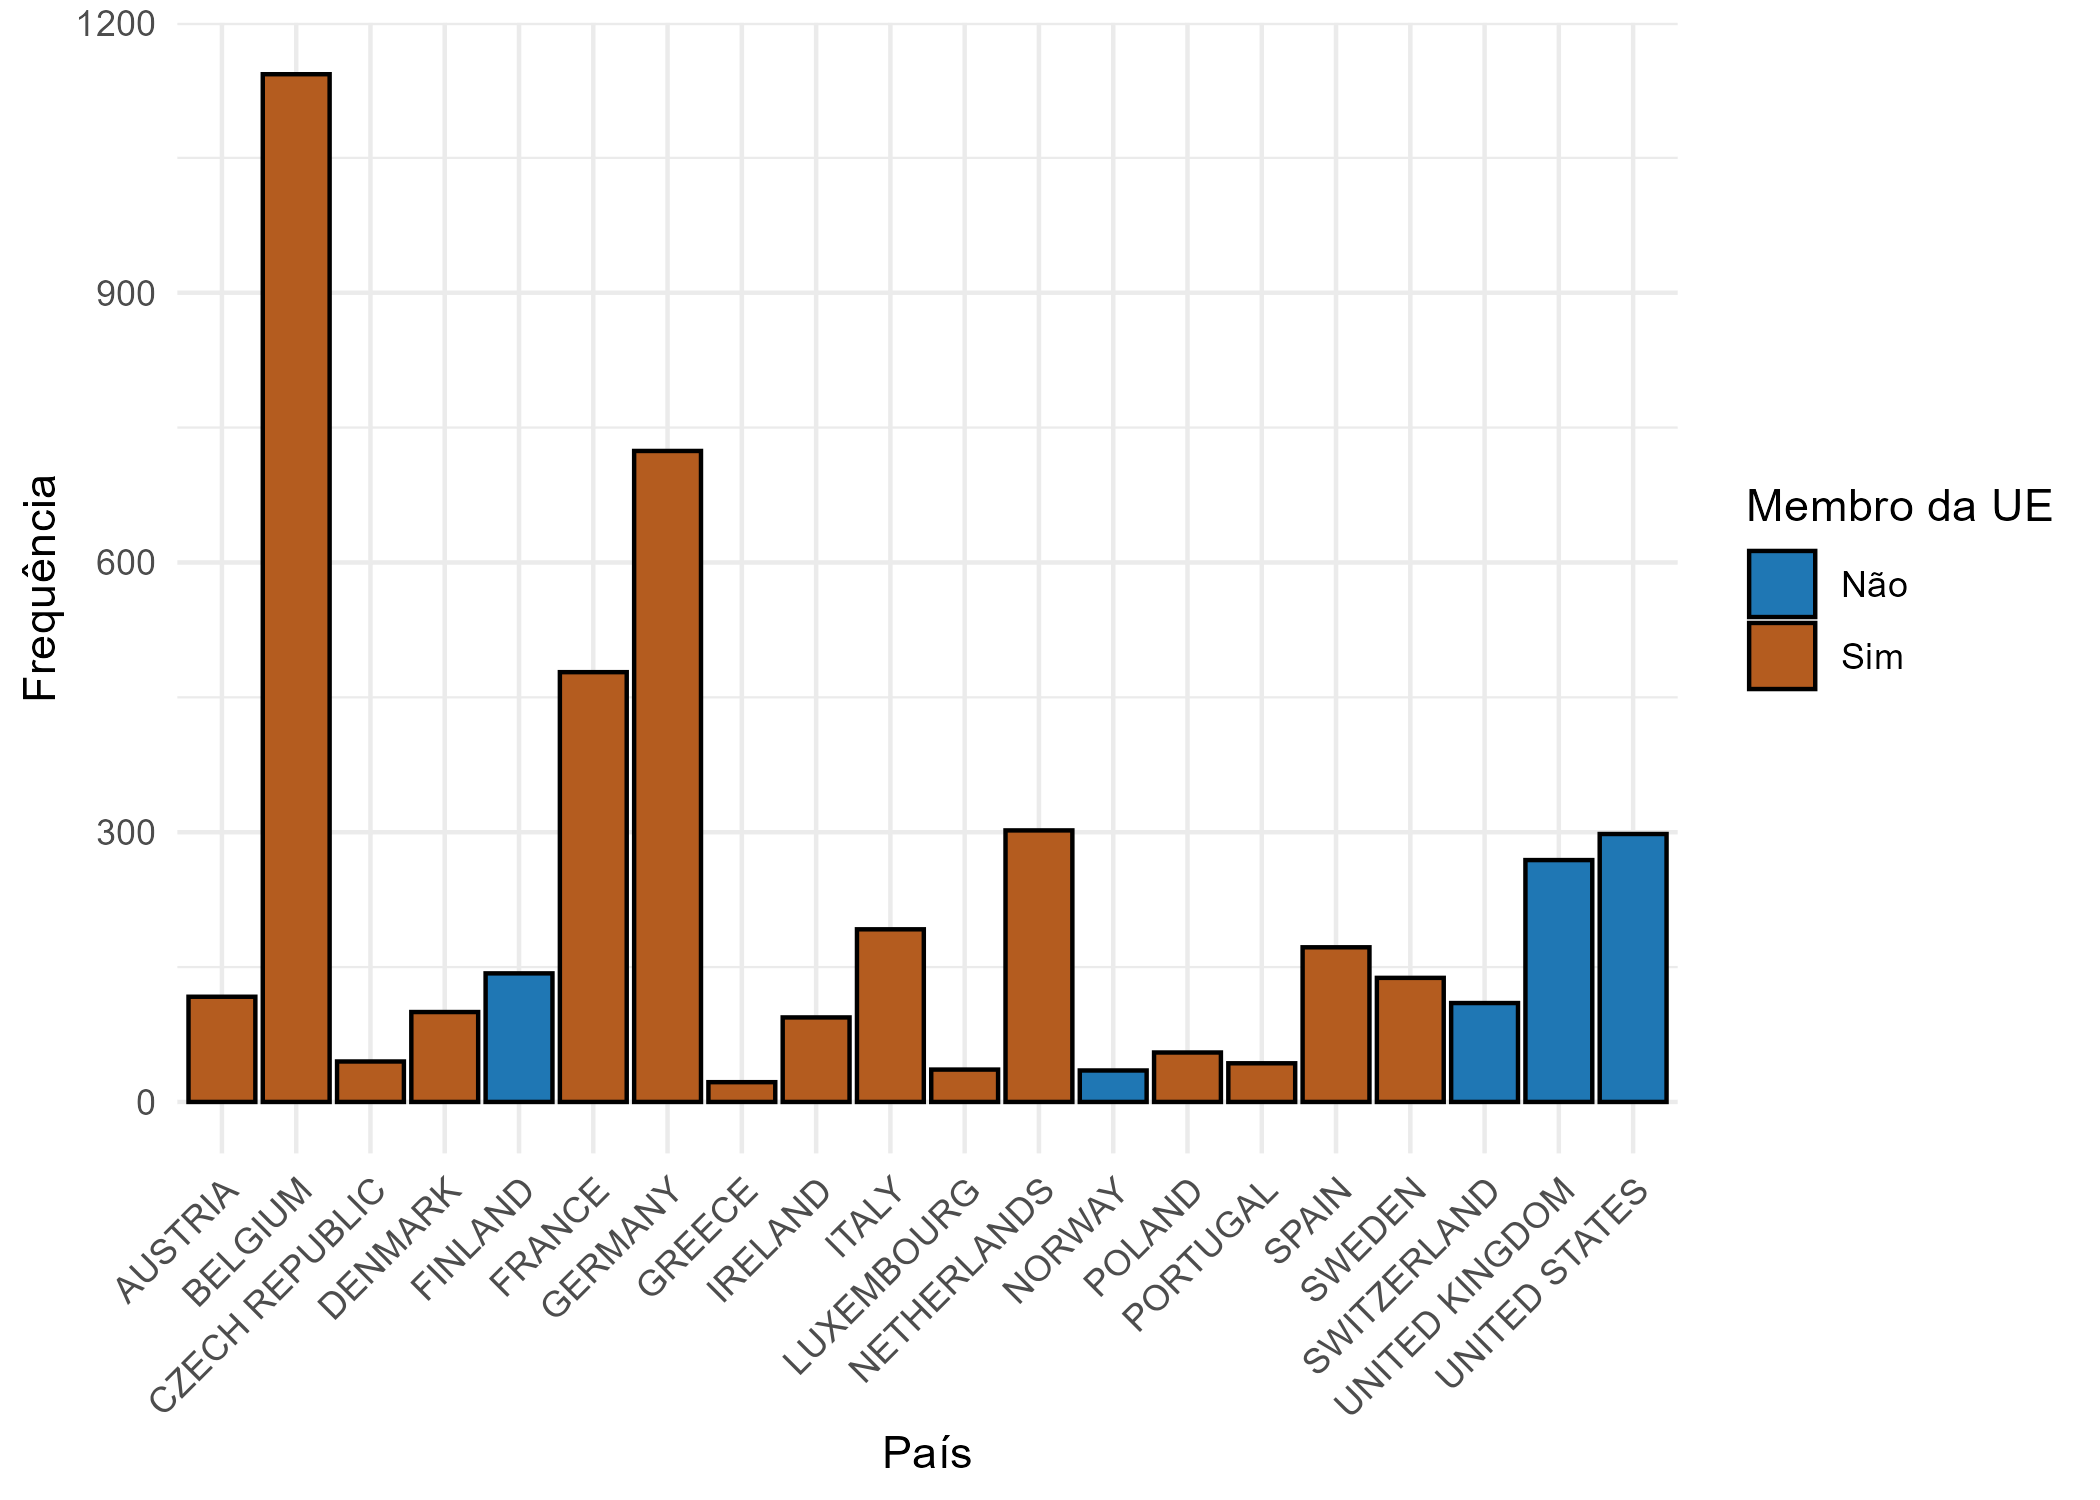
\includegraphics[width=0.9\textwidth]{figures/descriptives_lobbyists/barplot_country_distribution.png}
\caption{Top 20 países-sede (n = 4.516 organizações, totalizando 95,6\% do total de organizações)}
\label{fig:country_distribution}
\end{figure}

O fenômeno do \textit{venue-shopping} — a escolha estratégica do fórum mais favorável para exercer pressão — é central para entender essa distribuição \cite{kluver2015legislative}. A estrutura institucional da \acrshort{ue}, com poder decisório partilhado entre a Comissão, o Conselho e o Parlamento, incentiva os grupos de interesse a se estabelecerem nos locais onde podem monitorar e intervir mais eficazmente no ciclo político. A proeminência de países como Alemanha e França reflete não apenas a proximidade, mas também o peso político e econômico que exercem dentro da \acrshort{ue}.

Adicionalmente, a presença significativa de atores extracomunitários, que representam cerca de 20\% do total de organizações com sedes em 70 países (com destaque para os Estados Unidos, com 6,3\%), evidencia a importância da \acrshort{ue} como arena regulatória global. A atratividade do mercado europeu e o impacto de suas decisões incentivam atores internacionais a investir em uma presença local para influenciar a formulação de políticas que afetarão seus interesses. 

O recorte do top 20, que mostra uma cauda longa com muitos países de baixa frequência, reforça a ideia de que, embora o sistema seja permeável, os altos custos de manter uma operação de lobby eficaz na Europa centralizam a influência em atores com maiores recursos e localização estratégica.

% Distribuição temporal dos registros
Temporalmente, observa-se aceleração do registro de entidades após meados da década de 2010, com 2023 concentrando 17,9\% do total. Picos intermediários (2015--2016; 2020--2022) são compatíveis com ciclos legislativos, janelas regulatórias e alterações incrementais nos mecanismos de transparência.

\begin{figure}[!htbp]
\centering
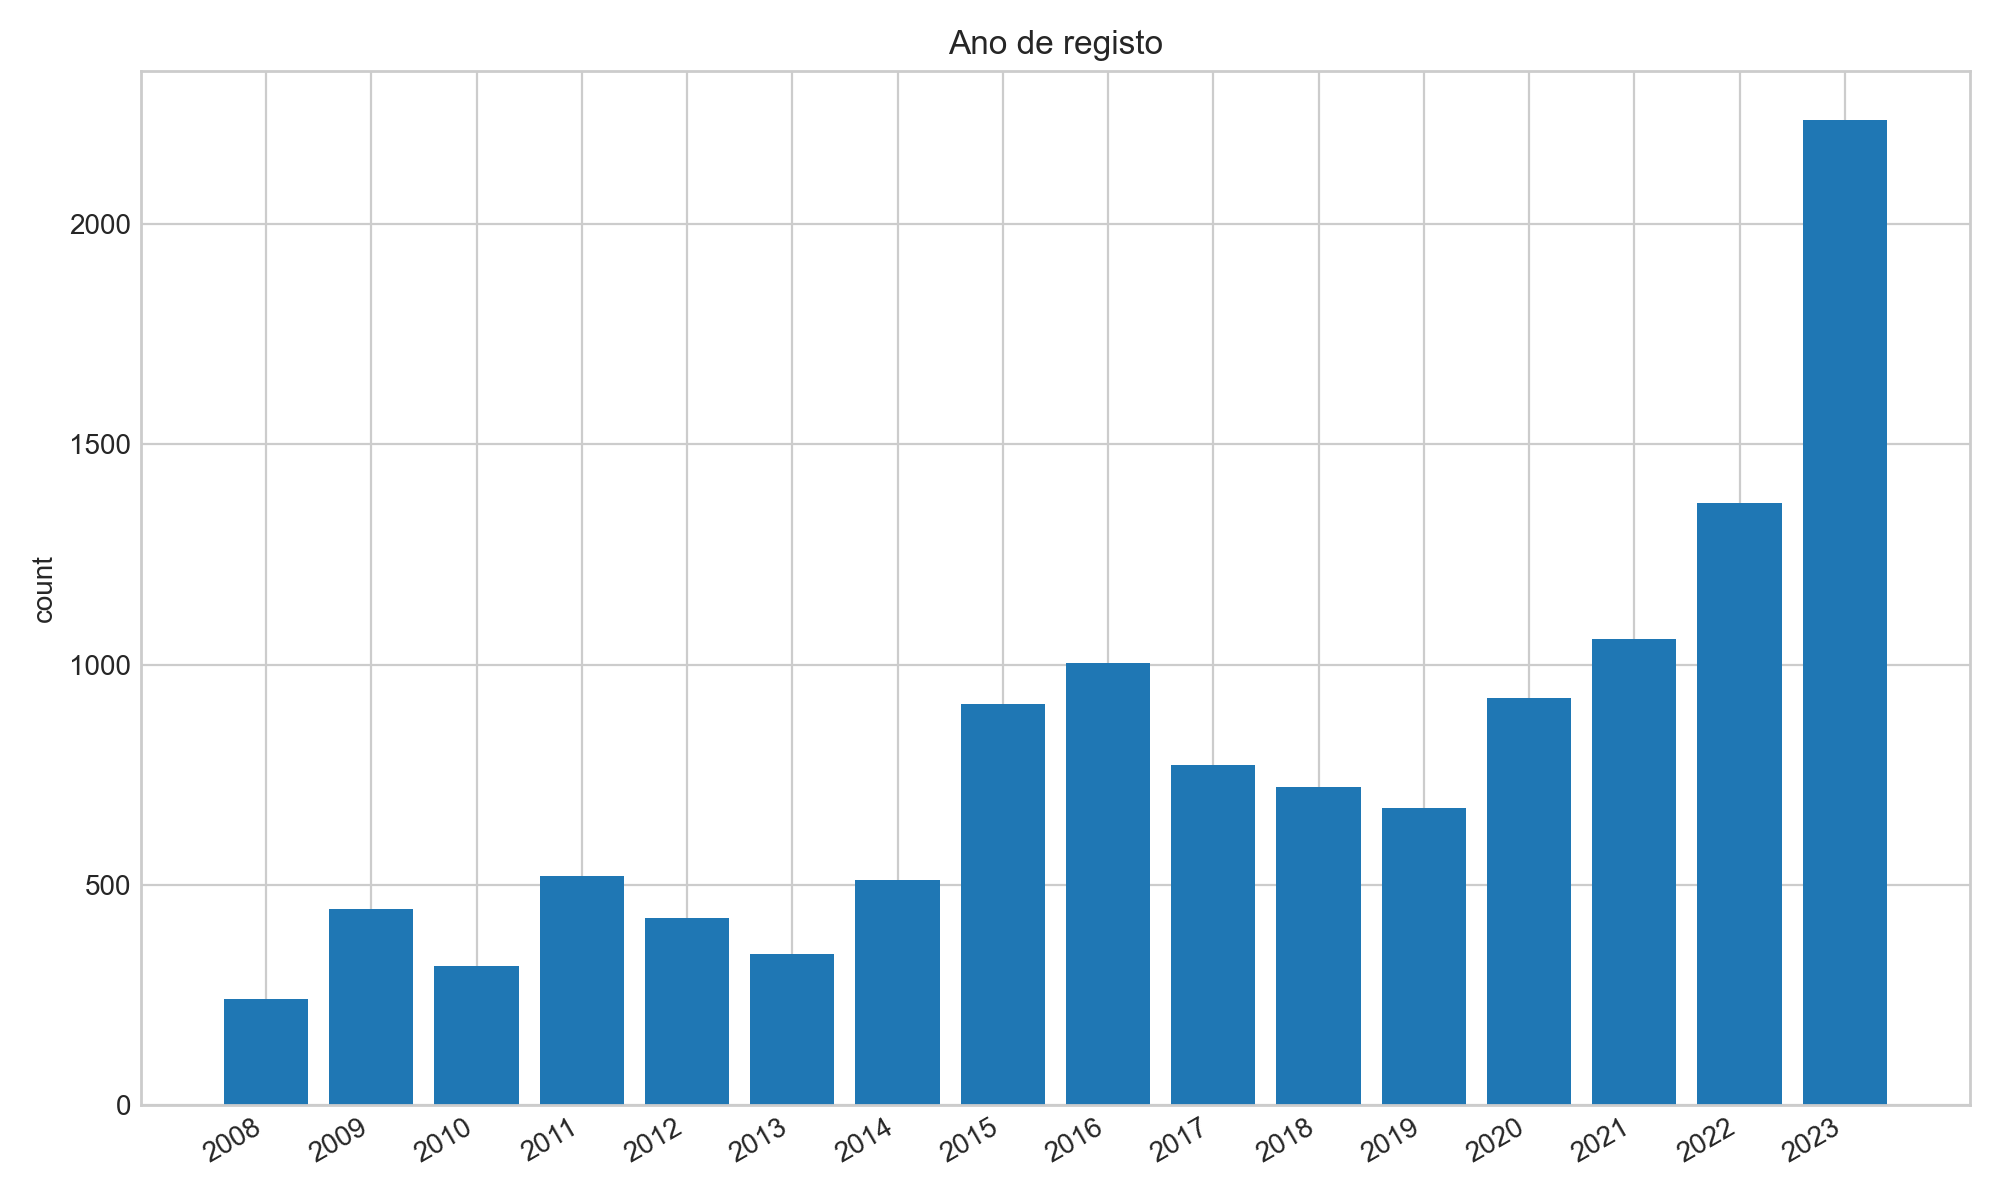
\includegraphics[width=0.75\textwidth]{figures/year_distribution.png}
\caption{Ano de registo}
\end{figure}

O padrão visual sugere crescimento estrutural recente do ecossistema de representação de interesses, possivelmente associado às agendas de transição digital e verde e à recomposição pós-pandemia.

% Distribuição temática
As incidências por domínio (Figura \ref{fig:theme_coverage}) destacam \textit{Economia e Comércio} (15\%), \textit{Tecnologia} (14,9\%) e \textit{Infraestrutura e Indústria} (14,4\%), seguidas por \textit{Tecnologia} (14,2\%) e \textit{Meio Ambiente e Clima} (13,8\%). Temas como \textit{Saúde} (9,8\%) e \textit{Educação} (8,1\%) são intermediários; \textit{Agricultura} (7,2\%) e \textit{Direitos Humanos} (6,2\%) têm menor incidência relativa.

\begin{figure}[!htbp]
\centering
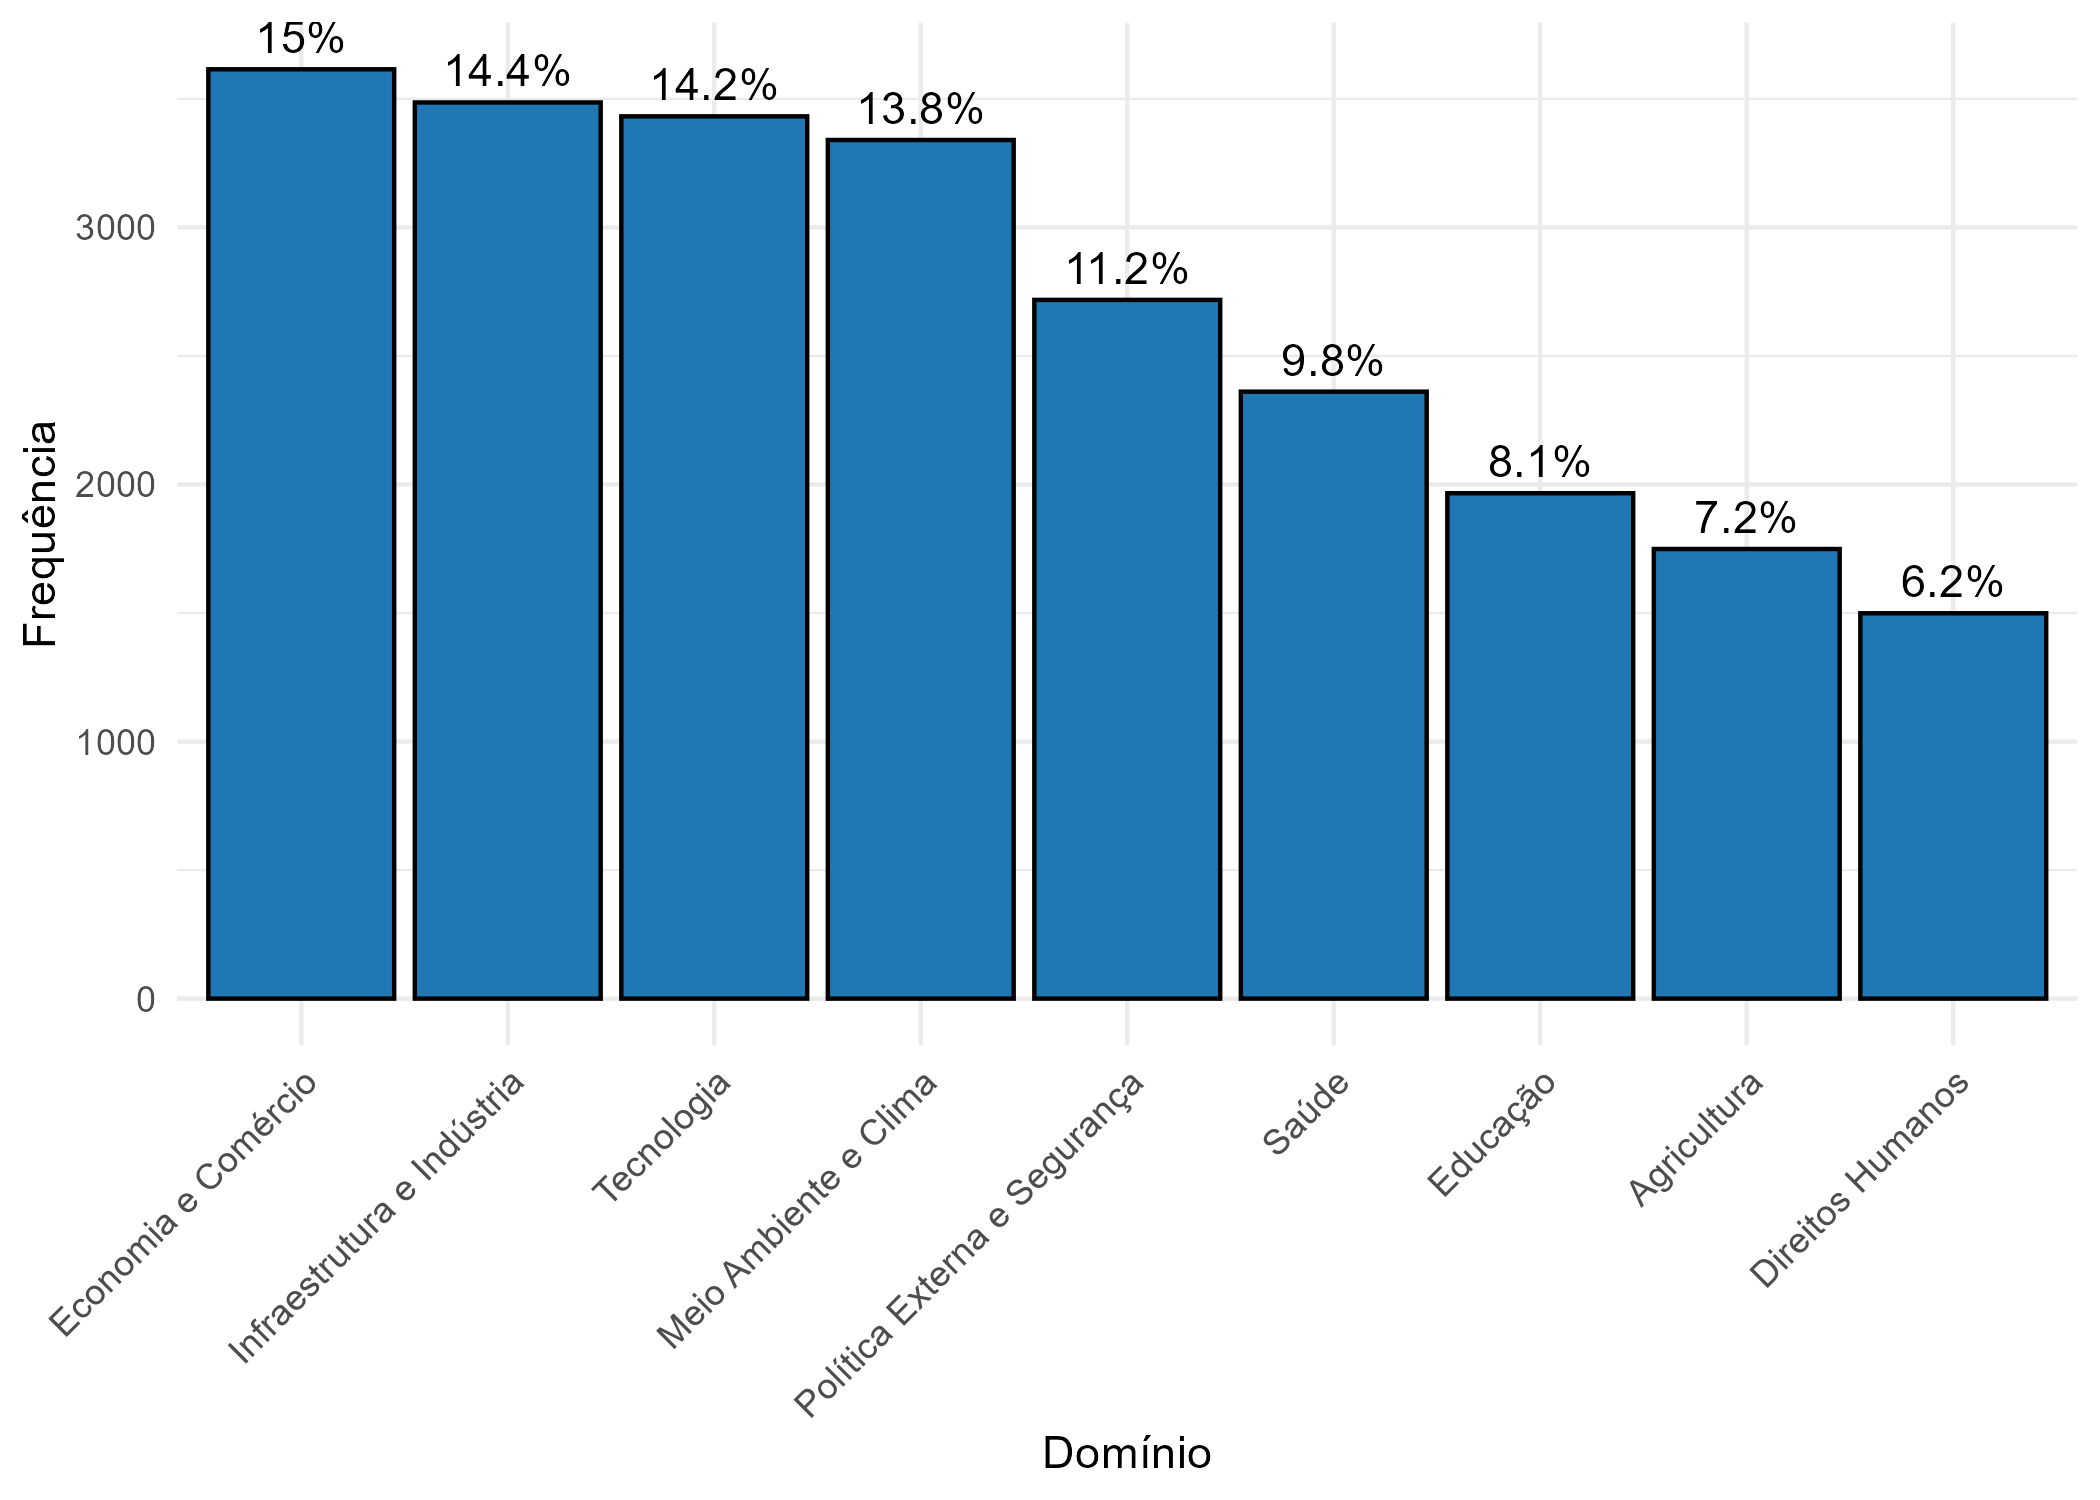
\includegraphics[width=0.9\textwidth]{figures/descriptives_lobbyists/barplot_domain_distribution.png}
\caption{Cobertura temática (proporção de entidades)}
\label{fig:theme_coverage}
\end{figure}

A distribuição temática (Figura \ref{fig:theme_coverage}) reflete uma concentração estratégica de esforços de lobby nas arenas de maior peso econômico e regulatório da União Europeia. A proeminência de domínios como "Economia e Comércio", "Infraestrutura e Indústria" e "Tecnologia" está alinhada com a literatura que demonstra uma correlação positiva entre a atividade de lobby e a saliência de um tema \cite{caldeira2000lobbying, baumgartner2010agendas}. São áreas onde as decisões políticas implicam altas consequências financeiras, mobilizando um volume expressivo de atores.

Adicionalmente, esses temas são caracterizados por uma elevada complexidade técnica. Este fator aumenta a demanda por informação especializada por parte dos decisores políticos, criando um vácuo que os lobistas buscam preencher para ganhar acesso e exercer influência, conforme sugere a literatura sobre o papel informacional do lobby \cite{kluver_informational_2012}. A própria agenda política da \acrshort{ue}, com iniciativas centrais como o Mercado Único Digital e o Pacto Ecológico Europeu, transforma esses domínios em focos de intensa atividade, corroborando a ideia de que os grupos de interesse são mais ativos nos temas em que o Estado também é mais atuante \cite{mahoney2008brussels}.

Em contraste, temas como "Direitos Humanos" e "Agricultura", embora relevantes, apresentam menor incidência relativa. Isso pode indicar que os interesses difusos ou setoriais dessas áreas enfrentam maiores desafios de ação coletiva ou utilizam estratégias de influência distintas, que não se refletem com a mesma intensidade no lobby direto. O padrão observado, portanto, sugere um ecossistema de lobby que responde de forma racional tanto aos incentivos econômicos quanto às necessidades informacionais geradas pela agenda regulatória da UE.

\begin{figure}[!htbp]
\centering
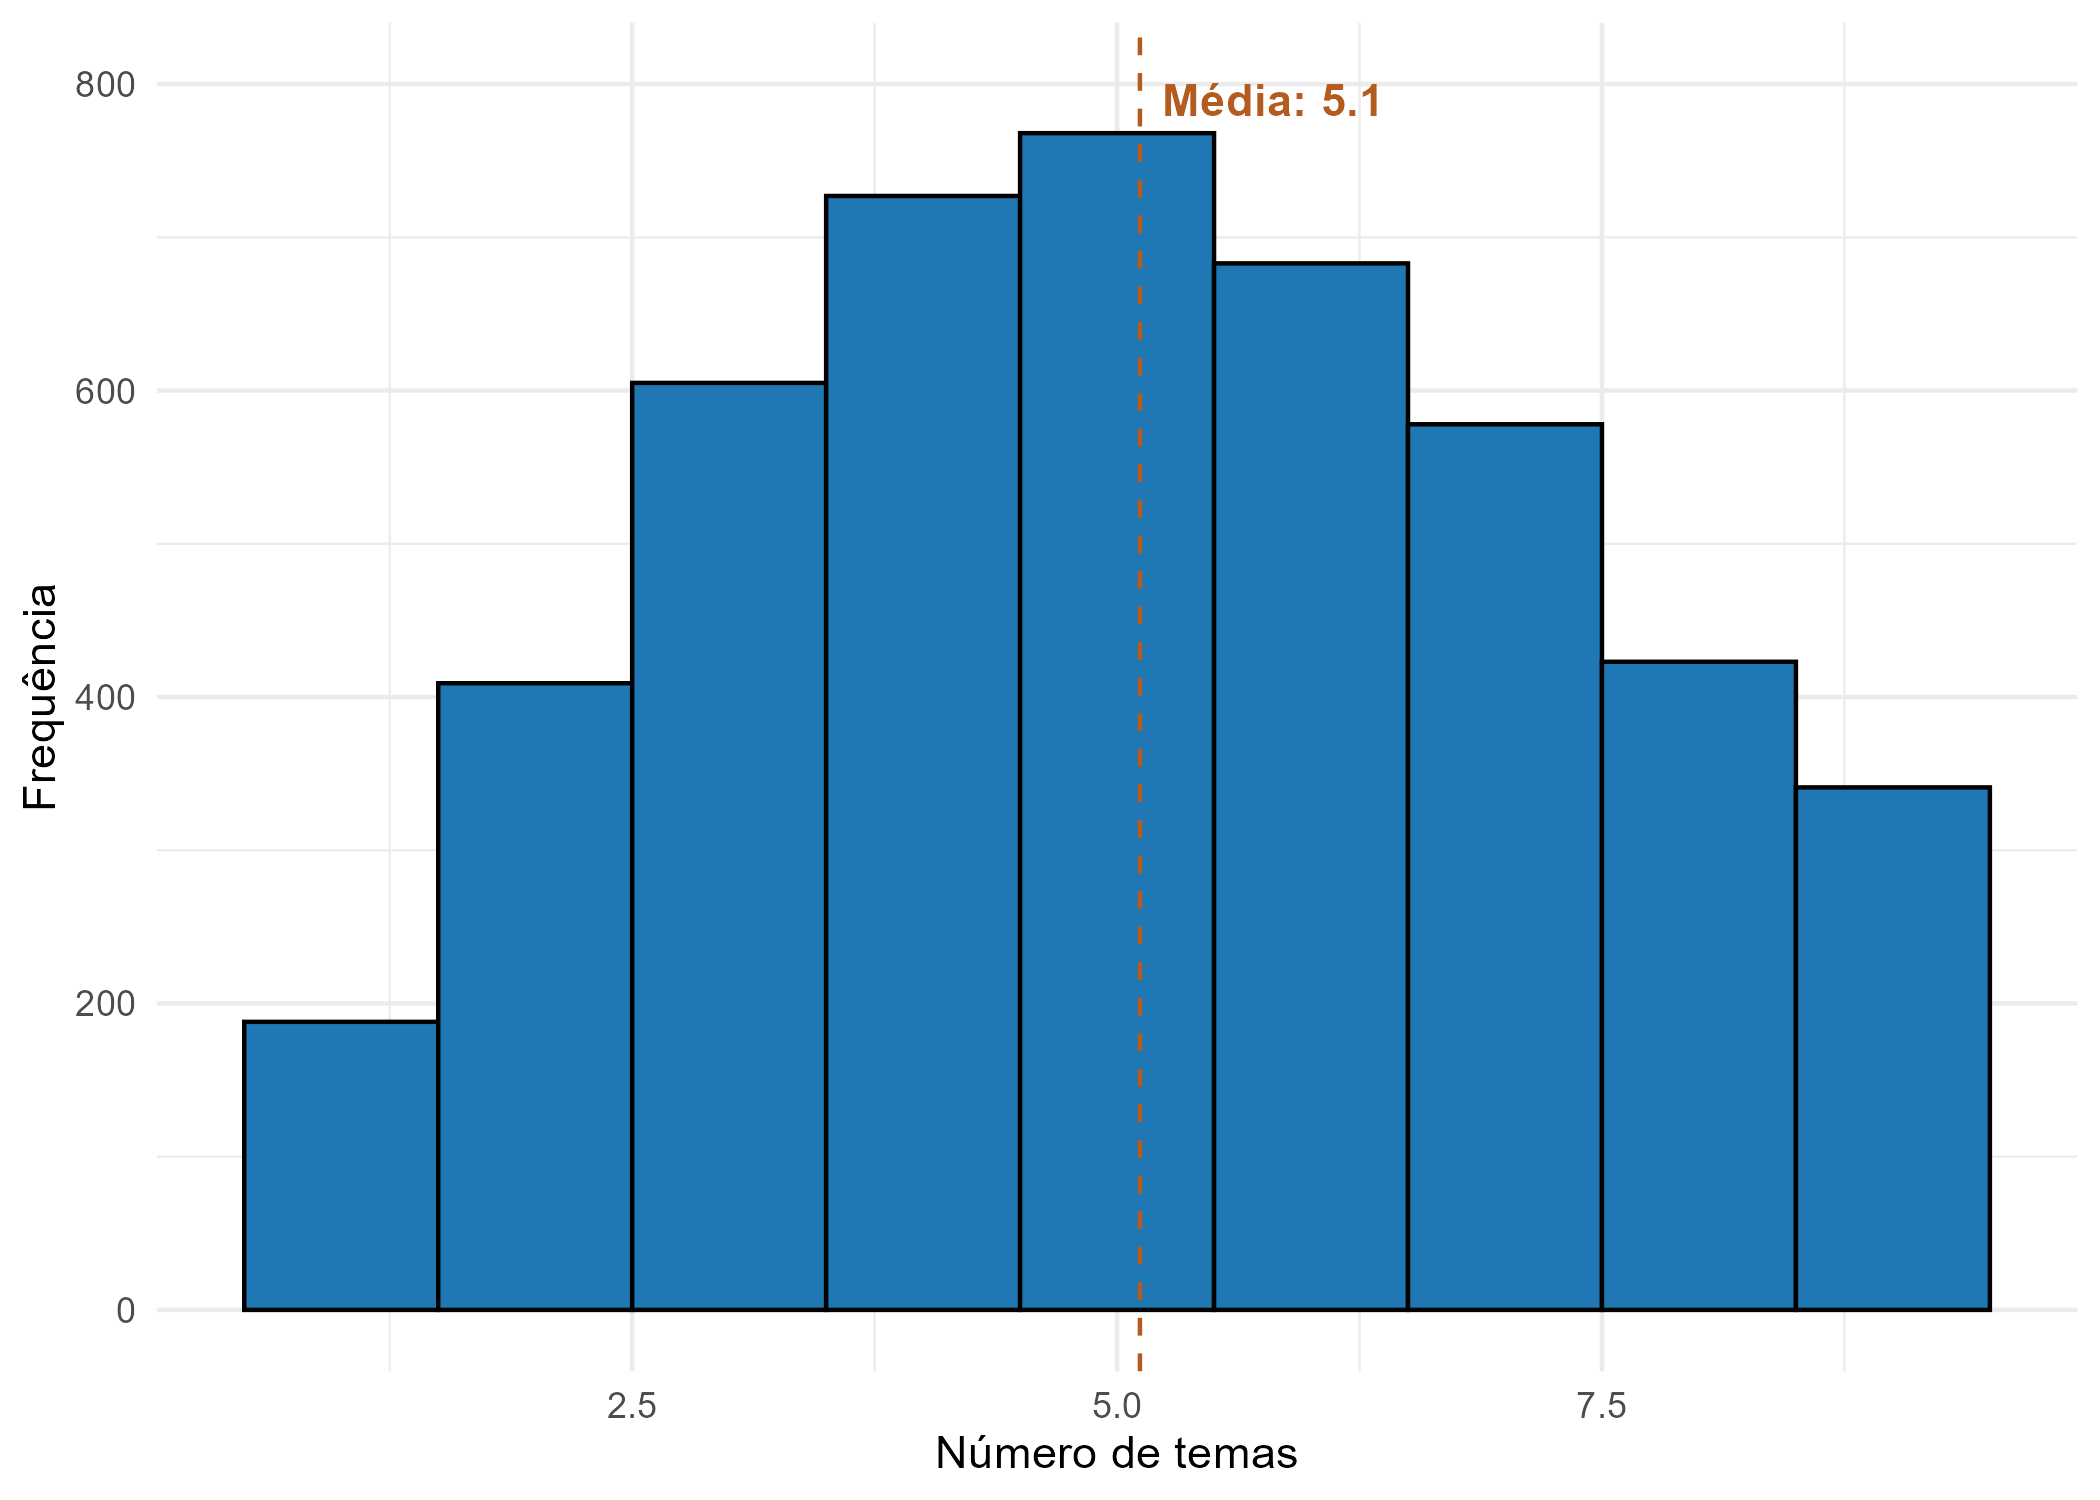
\includegraphics[width=0.75\textwidth]{figures/descriptives_lobbyists/histogram_themes_per_lobbyist.png}
\caption{Número de temas por lobista}
\label{fig:themes_per_lobbyist_hist}
\end{figure}

A análise da diversidade temática das organizações (Figura \ref{fig:themes_per_lobbyist_hist}) revela que a maioria dos lobistas atua em múltiplas frentes. A distribuição, que se assemelha a uma curva normal com média de 5,1 temas por organização, demonstra a coexistência de estratégias especializadas (focadas em poucos temas) e generalistas. Contudo, o padrão dominante é o de uma abordagem multi-temática, onde as organizações cobrem um portfólio de 3 a 7 áreas de interesse.

Este achado dialoga diretamente com o debate na literatura sobre os recursos mais valiosos para o lobby: expertise ("o que você sabe") versus conexões ("quem você conhece") \cite{bertrand2014whom}. A presença de atores especializados sugere uma aposta na expertise técnica como via de influência, especialmente em domínios de alta complexidade \cite{kluver_informational_2012}. Por outro lado, a predominância de atores multi-temáticos indica que uma estratégia mais ampla, possivelmente baseada em redes de contatos e na capacidade de adaptação a diferentes arenas políticas, é a norma no complexo ambiente institucional da \acrshort{ue}. A governança multinível e a interconexão de políticas na Europa podem incentivar as organizações a não se limitarem a um único nicho, buscando pontos de acesso em diferentes comissões e agências \cite{coen2019legislative}.

Em conjunto, os resultados descritivos apontam para um ecossistema plural, geograficamente ancorado em polos institucionais centrais, com dinamismo temporal recente e agendas orientadas por digitalização, competitividade industrial e sustentabilidade. Esses padrões informam as escolhas de especificação nos capítulos seguintes, notadamente a estratificação por perfis organizacionais, a construção de domínios temáticos e o controle para tendências temporais.


Os resultados descritivos delineiam um panorama abrangente do universo de lobistas registados junto às instituições europeias. Em primeiro lugar, a distribuição por categoria revela a coexistência de diferentes perfis organizacionais (\textit{Empresas}, \textit{\acrshort{ong}s} e \textit{Outros}), com magnitudes comparáveis entre atores empresariais e organizações da sociedade civil. Essa composição é compatível com a literatura sobre pluralismo organizacional e competição por acesso institucional no contexto da \acrshort{ue}, sugerindo um campo de ação onde interesses difusos e concentrados buscam simultaneamente agenda e influência.

Em síntese, as evidências descritivas apontam para um ecossistema plural, geograficamente ancorado em polos institucionais centrais, com dinamismo temporal recente e agendas orientadas por digitalização, competitividade industrial e sustentabilidade. Esses padrões informam as escolhas de especificação nos capítulos seguintes, notadamente a estratificação por perfis organizacionais, a construção de domínios temáticos e o controle para tendências temporais.


\section{Análise descritiva do tratamento}
\label{sec:resultados_descritica}

Esta seção apresenta uma análise descritiva sistemática dos dados utilizados para investigar os efeitos do lobbying na atividade parlamentar dos deputados do Parlamento Europeu. A abordagem adotada segue uma estratégia analítica multinível, iniciando com padrões agregados gerais e progredindo para análises desagregadas mais específicas. Esta progressão metodológica permite compreender tanto as tendências globais quanto os mecanismos específicos que operam no nível individual e temporal.

O conjunto de dados constitui um painel balanceado que combina informações sobre atividade parlamentar (perguntas) e intensidade de lobbying (reuniões) para 1.353 deputados ao longo de 63 meses, de julho de 2019 a novembro de 2024 em 9 domínios de política pública. Esta estrutura temporal permite capturar variações tanto na dimensão \textit{cross-sectional} (entre deputados e domínios) quanto longitudinal (evolução temporal), fornecendo a base empírica necessária para estratégias de identificação causal robustas.

Considerando a unidade de análise a tríade MEP-domínio-mês, temos 767.151 observações com taxa de completude de 100\%. Esta estrutura balanceada é metodologicamente vantajosa, pois elimina preocupações com viés de seleção decorrente de atrito amostral e garante que as estimativas não sejam distorcidas por padrões de observações ausentes.

A cobertura temporal de julho de 2019 a novembro de 2024 é particularmente relevante por abranger períodos de intensa atividade legislativa europeia, incluindo a transição entre legislaturas e eventos político-econômicos significativos. Destaca-se, nesse intervalo, o impacto da pandemia de COVID-19, que afetou profundamente tanto a dinâmica da atividade parlamentar quanto as estratégias de lobbying. A pandemia resultou em mudanças substanciais nos modos de trabalho do Parlamento Europeu, com a adoção de sessões remotas e restrições a reuniões presenciais, o que pode ter alterado padrões de interação entre deputados e grupos de interesse. Assim, a análise cobre não apenas períodos de normalidade institucional, mas também um contexto de crise sanitária global, permitindo investigar como choques exógenos desse tipo influenciam o comportamento político e o lobbying.

A \autoref{fig:time_series} apresenta a evolução temporal das variáveis principais no nível mais agregado, revelando padrões que são fundamentais para compreender a dinâmica do sistema político europeu ao longo do período estudado.

\begin{figure}[htbp]
\centering
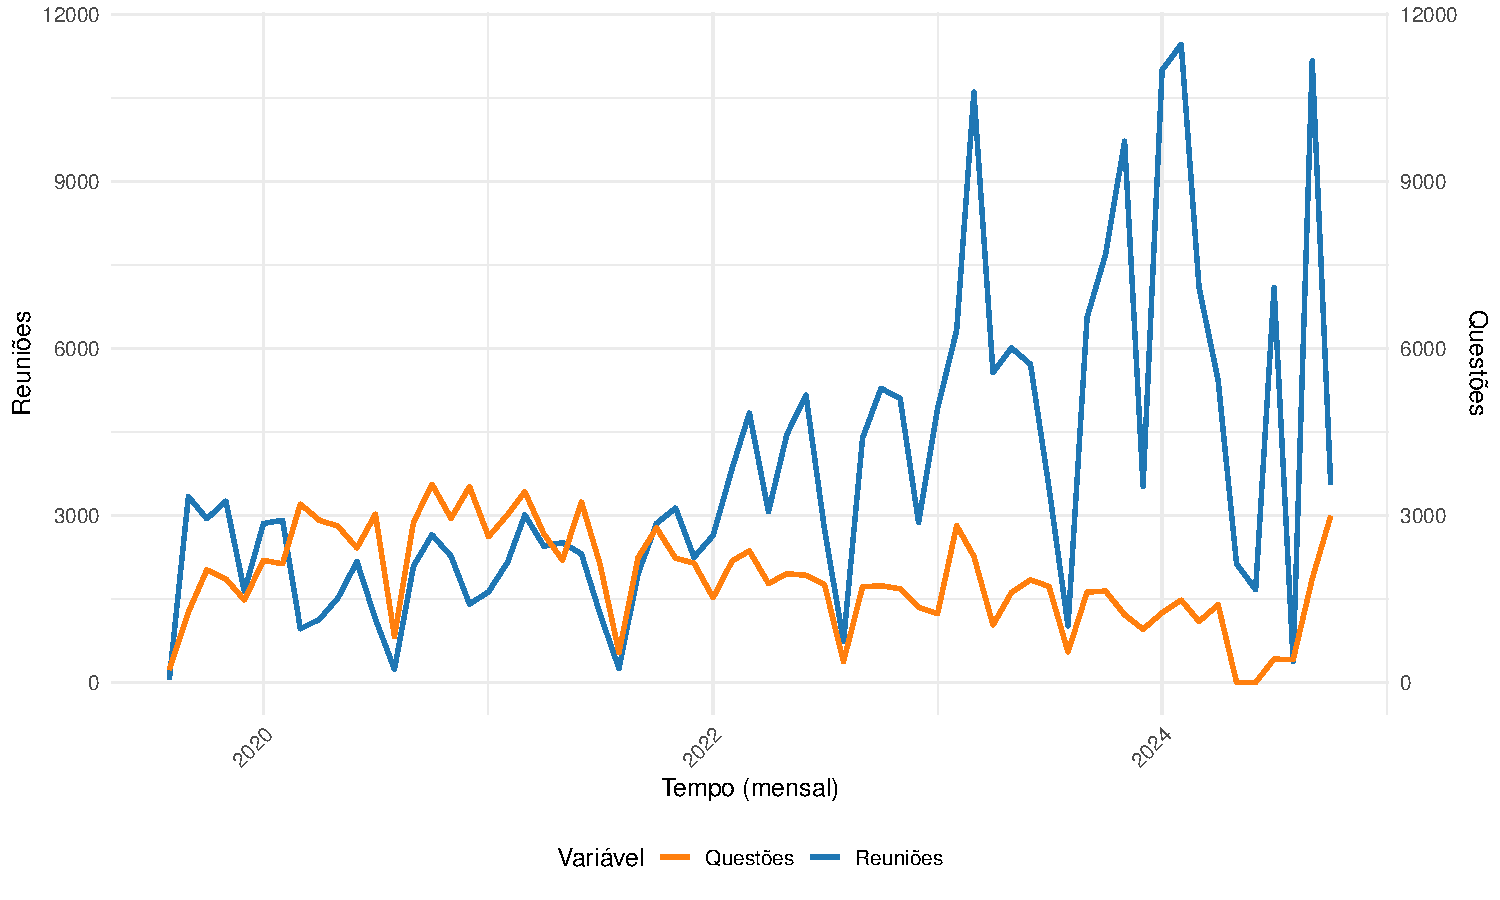
\includegraphics[width=\textwidth]{figures/fig1_time_series_meetings_questions.pdf}
\caption{Evolução temporal da atividade parlamentar e de lobbying}
\label{fig:time_series}
% \note{O painel superior esquerdo mostra os totais mensais agregados de perguntas e reuniões. O painel superior direito apresenta as médias mensais por observação MEP-domínio. O painel inferior esquerdo mostra a evolução da proporção de observações com atividade de lobbying. O painel inferior direito apresenta a estabilidade da correlação contemporânea entre as variáveis ao longo do tempo.}
\end{figure}

A análise temporal revela quatro padrões empiricamente relevantes. Primeiro, observa-se uma \textbf{tendência crescente} em ambas as variáveis ao longo do período, sugerindo intensificação tanto da atividade parlamentar quanto do lobbying. Segundo, existe clara \textbf{sazonalidade} relacionada ao calendário parlamentar, com reduções sistemáticas durante períodos de recesso. Terceiro, identificam-se \textbf{picos de atividade} que coincidem com discussões de legislação relevante em domínios específicos, indicando resposta coordenada do sistema político. Quarto, a \textbf{correlação contemporânea} entre perguntas e reuniões permanece relativamente estável ao longo do tempo, sugerindo estabilidade estrutural na relação entre as variáveis.

% não há exatamente essa tendência cerescente...


Estes padrões temporais têm implicações metodológicas importantes. A presença de tendências temporais justifica a inclusão de efeitos fixos de tempo nas especificações econométricas para controlar choques temporais comuns. A sazonalidade observada valida a escolha da frequência mensal como unidade temporal, capturando variações de curto prazo sem introduzir ruído excessivo. A estabilidade da correlação fornece evidência preliminar contra quebras estruturais que poderiam comprometer a validade das estimativas.

% \subsection{Padrões de participação: análise agregada por deputado}

Complementando a análise temporal, é fundamental examinar os padrões de participação no nível individual dos deputados. Esta perspectiva agregada revela a distribuição da atividade de lobbying entre os parlamentares e fornece insights sobre a concentração e heterogeneidade dos fenômenos estudados.



As \autoref{fig:proportion_meetings}, \autoref{fig:correlation_meetings_questions} e \autoref{fig:meetings_hist} apresentam uma análise dos padrões de participação agregados por deputado, revelando aspectos da distribuição da atividade de lobbying no Parlamento Europeu que impactam a identificação causal.

% \begin{figure}[htbp]
% \centering
% 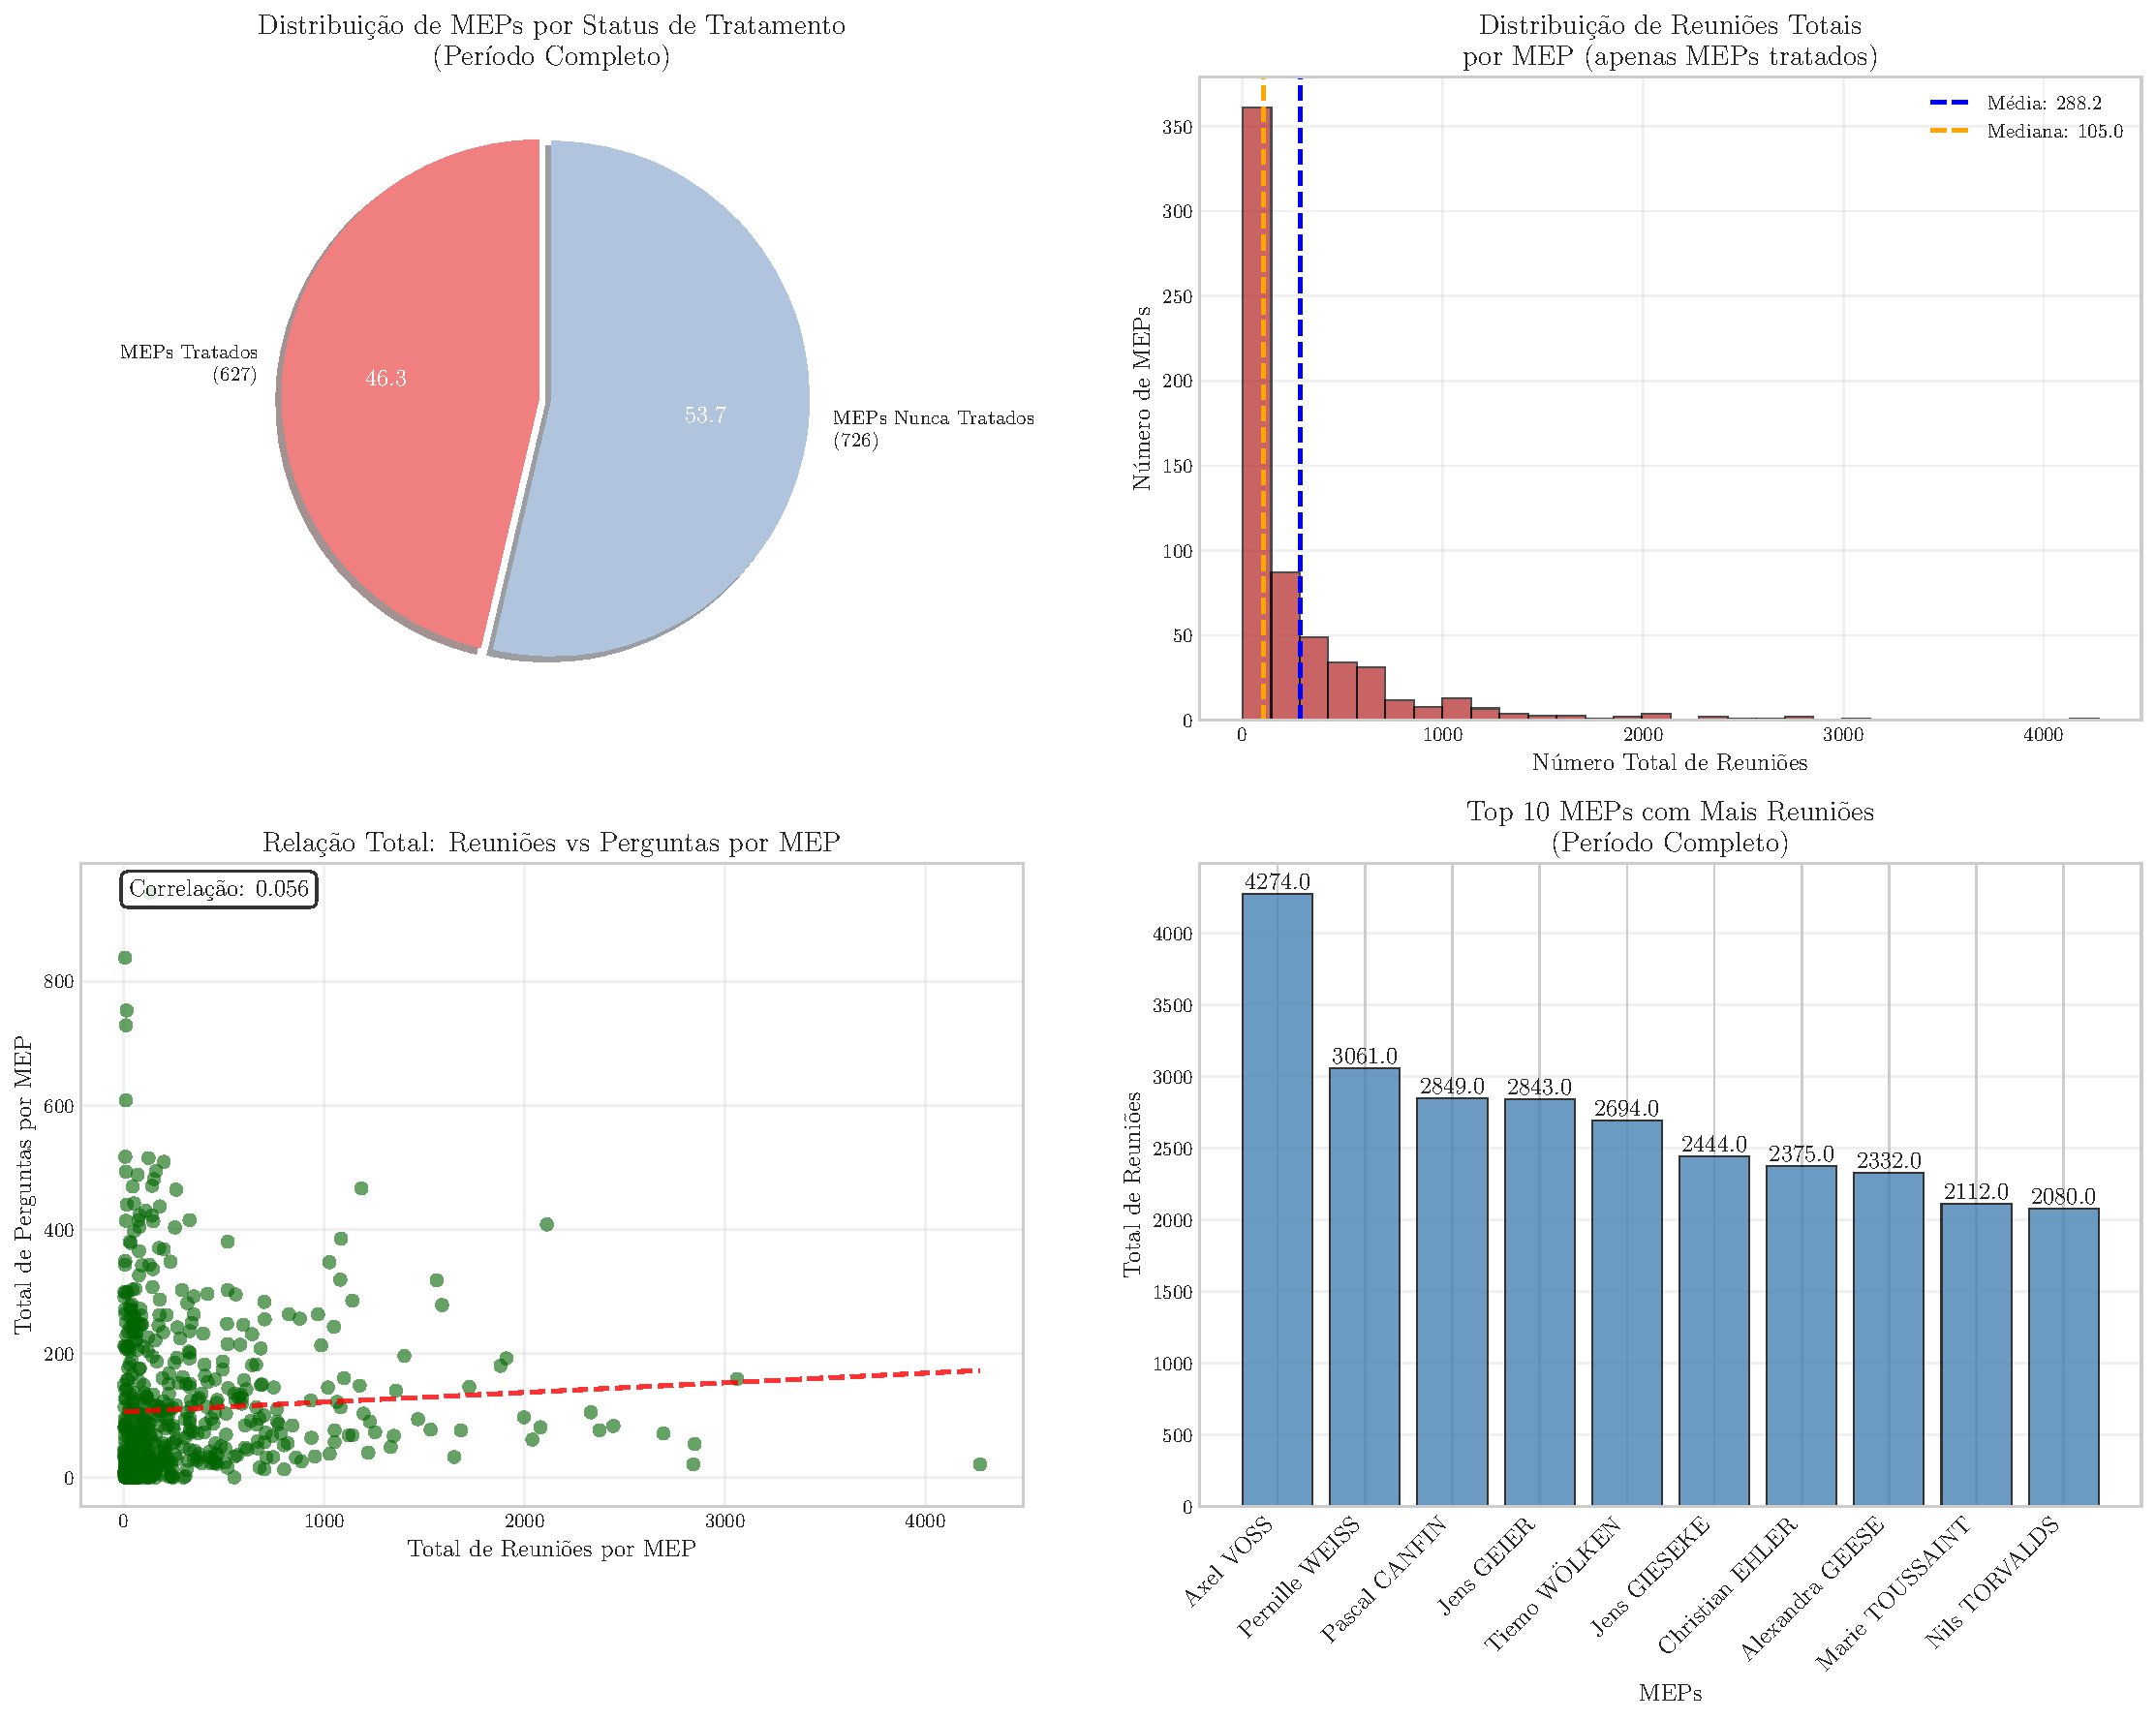
\includegraphics[width=\textwidth]{figures/fig6_mep_aggregated_analysis.pdf}
% \caption{Análise agregada por MEP: distribuição e intensidade do tratamento}
% \label{fig:mep_aggregated}
% \note{O painel superior esquerdo mostra a proporção de deputados que receberam pelo menos uma reunião de lobbying durante todo o período. O painel superior direito apresenta a distribuição da intensidade total de reuniões entre deputados tratados. O painel inferior esquerdo examina a relação agregada entre reuniões e perguntas totais por deputado. O painel inferior direito identifica os deputados mais ativos em termos de recepção de lobbying.}
% \end{figure}



% \subsubsection{Distribuição do tratamento entre deputados}

\begin{figure}[htbp]
    \centering
    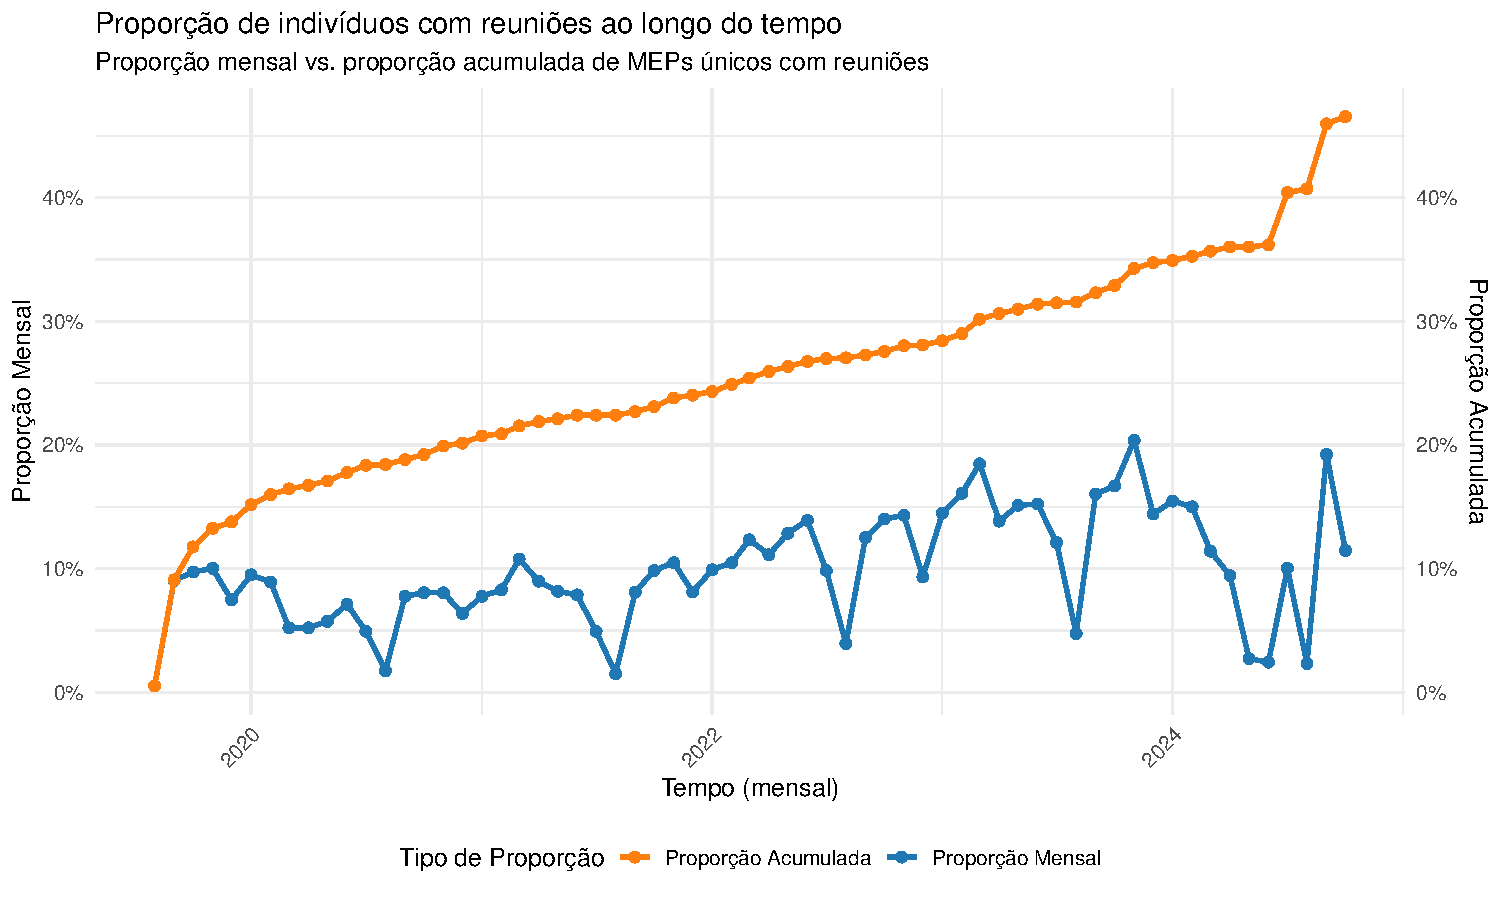
\includegraphics[width=\textwidth]{figures/fig2_proportion_meetings.pdf}
    \caption{Evolução temporal da proporção de \acrshort{mpe}s que participaram de reuniões de lobbying}
    \label{fig:proportion_meetings}
    % \note{O painel superior esquerdo mostra os totais mensais agregados de perguntas e reuniões. O painel superior direito apresenta as médias mensais por observação MEP-domínio. O painel inferior esquerdo mostra a evolução da proporção de observações com atividade de lobbying. O painel inferior direito apresenta a estabilidade da correlação contemporânea entre as variáveis ao longo do tempo.}
\end{figure}

\begin{figure}[htbp]
    \centering
    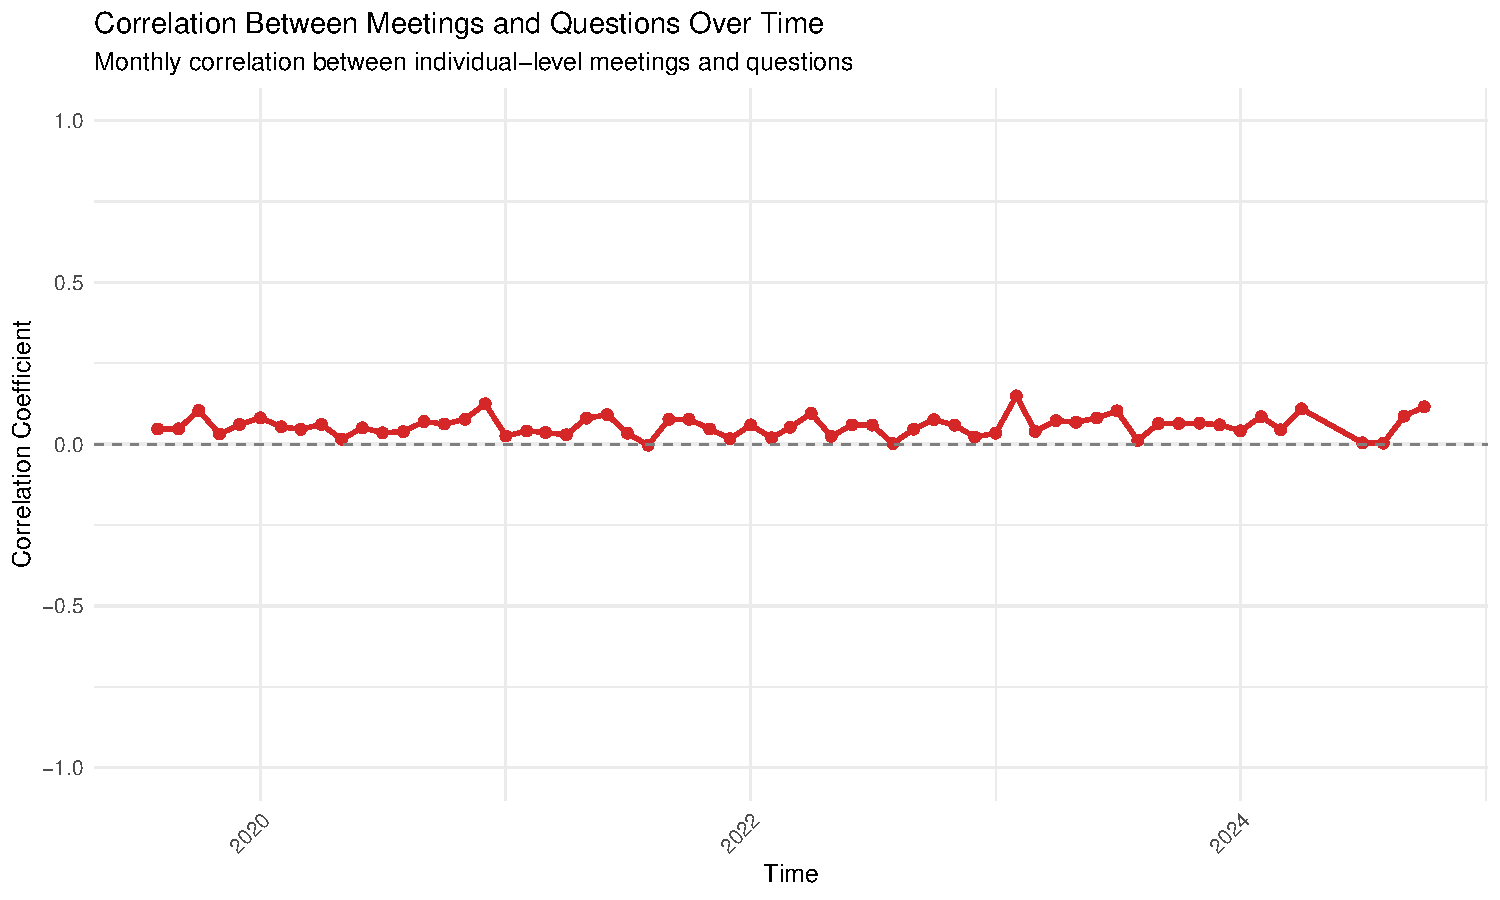
\includegraphics[width=\textwidth]{figures/fig3_correlation_meetings_questions.pdf}
    \caption{Evolução temporal da correlação entre reuniões e perguntas}
    \label{fig:correlation_meetings_questions}
    % \note{O painel superior esquerdo mostra os totais mensais agregados de perguntas e reuniões. O painel superior direito apresenta as médias mensais por observação MEP-domínio. O painel inferior esquerdo mostra a evolução da proporção de observações com atividade de lobbying. O painel inferior direito apresenta a estabilidade da correlação contemporânea entre as variáveis ao longo do tempo.}
\end{figure}

\begin{figure}[htbp]
    \centering
    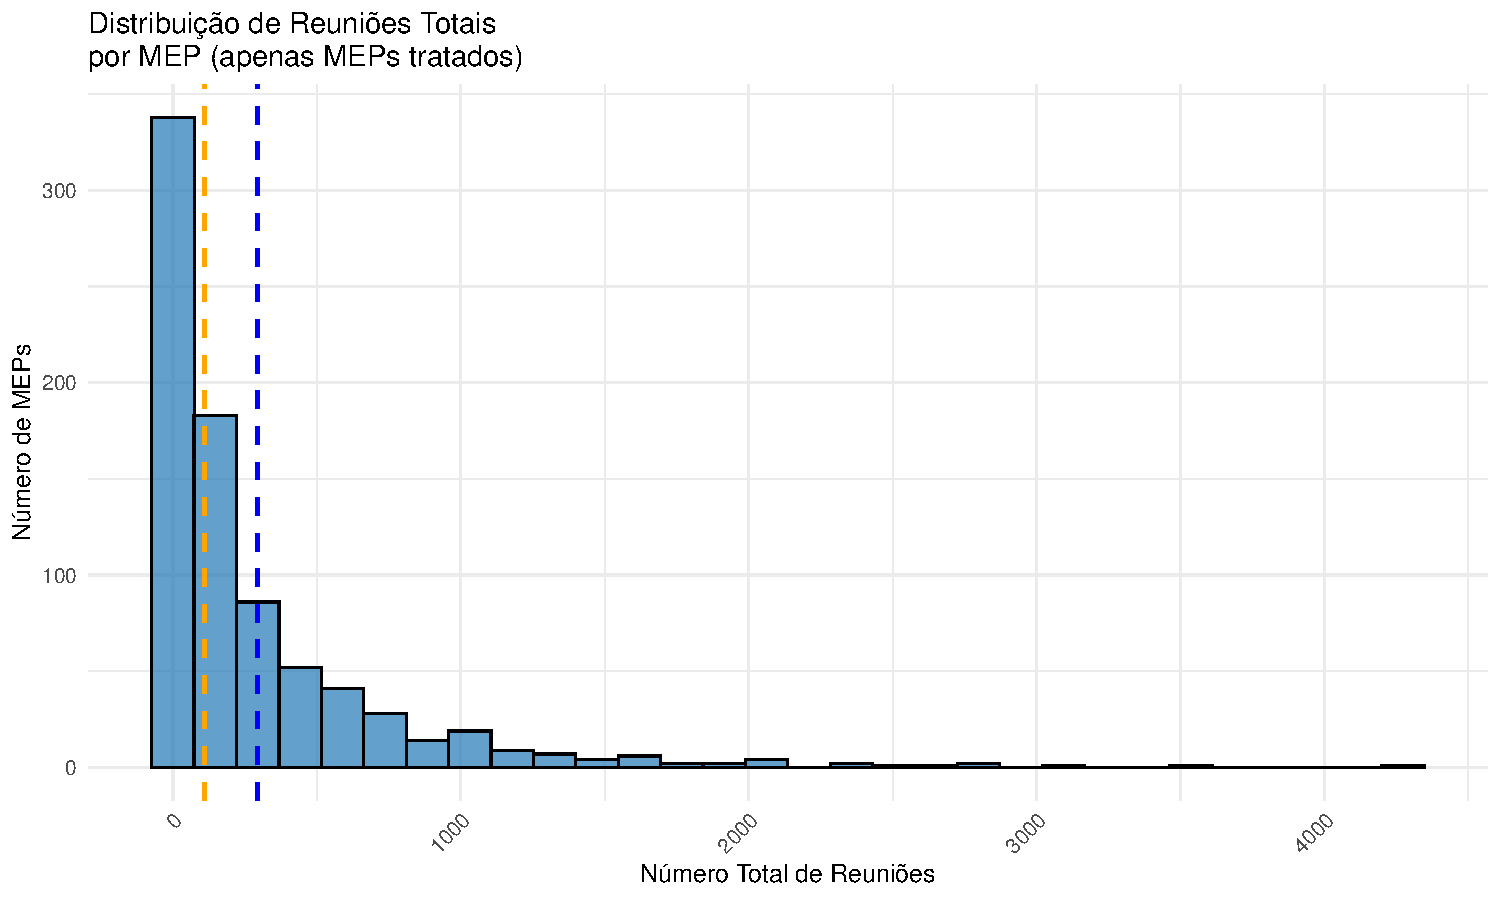
\includegraphics[width=\textwidth]{figures/fig3.1_meetings_hist.pdf}
    \caption{Distribuição de reuniões por \acrshort{mpe}}
    \label{fig:meetings_hist}
    % \note{O painel superior esquerdo mostra os totais mensais agregados de perguntas e reuniões. O painel superior direito apresenta as médias mensais por observação MEP-domínio. O painel inferior esquerdo mostra a evolução da proporção de observações com atividade de lobbying. O painel inferior direito apresenta a estabilidade da correlação contemporânea entre as variáveis ao longo do tempo.}
\end{figure}


A análise revela três características fundamentais da distribuição de tratamento. Primeiro, existe \textbf{participação substancial mas não universal}: 46,3\% dos deputados (637 de 1.353) receberam pelo menos uma reunião de lobbying durante o período estudado. Esta proporção indica que o lobbying é um fenômeno disseminado mas não ubíquo no sistema parlamentar europeu.

Segundo, observa-se \textbf{concentração extrema} na intensidade de tratamento. Entre os deputados que receberam lobbying, a distribuição é altamente assimétrica: enquanto a mediana é de 105 reuniões por deputado, a média é de 288,2 reuniões, indicando que uma minoria de parlamentares concentra uma proporção desproporcional da atividade lobista. O caso extremo de um deputado com 4.274 reuniões ilustra esta concentração.

Terceiro, a \textbf{correlação agregada} entre reuniões e perguntas totais por deputado é surpreendentemente baixa (0,056), contrastando com correlações mais elevadas observadas no nível temporal. Este padrão sugere que os efeitos do lobbying podem ser mais evidentes em frequências temporais específicas do que em padrões de atividade agregados de longo prazo.

% \paragraph{Implicações para a estratégia empírica}

Estes padrões agregados têm implicações importantes para a identificação causal. A concentração do tratamento em uma minoria de deputados sugere que estratégias de identificação baseadas em variação cross-sectional podem sofrer de poder estatístico limitado. Simultaneamente, a variação substancial na intensidade de tratamento entre deputados tratados fornece fonte valiosa de identificação para estimativas de dose-resposta.

A baixa correlação agregada, combinada com correlações temporais mais elevadas, indica que a identificação causal pode beneficiar-se de estratégias que explorem variação temporal within-individual rather than cross-sectional between-individual. Esta evidência preliminar orienta a especificação de modelos com efeitos fixos de deputado para controlar heterogeneidade não observada time-invariant.

\begin{table}[htbp]
\centering
\caption{Estatísticas agregadas de tratamento por deputado}
\label{tab:mep_treatment_stats}
\begin{tabular}{lr}
\toprule
\textbf{Estatística} & \textbf{Valor} \\
\midrule
Total de deputados únicos & 1{,}353 \\
Deputados que receberam tratamento & 627 \\
Taxa de tratamento por deputado (\%) & 46{,}3\% \\
\midrule
\textbf{Entre deputados tratados:} & \\
Reuniões médias por deputado & 288{,}2 \\
Reuniões medianas por deputado & 105{,}0 \\
Desvio padrão & 468{,}9 \\
Deputado mais ativo (reuniões) & 4{,}274 \\
\midrule
\textbf{Correlação agregada:} & \\
Correlação reuniões-perguntas & 0{,}056 \\
\bottomrule
\end{tabular}
\end{table}

\subsection{Heterogeneidade entre domínios de política pública}

A terceira dimensão da análise agregada examina a variação entre domínios de política pública. Esta heterogeneidade setorial é teoricamente relevante porque diferentes áreas de política podem apresentar características distintas em termos de complexidade técnica, interesse econômico e organização de grupos de pressão, afetando tanto a demanda por lobbying quanto a responsividade parlamentar.

% \paragraph{Padrões de tratamento por domínio}

A \autoref{fig:domain_treatment} apresenta uma análise sistemática da variação inter-domínios em múltiplas dimensões: penetração, volume e intensidade do tratamento, bem como padrões temporais de iniciação.


\begin{table}[htbp]
    \centering
    \caption{Taxa de tratamento por domínio: deputados únicos que receberam lobbying}
    \label{tab:domain_treatment_rates}
    \begin{tabular}{lrrr}
    \toprule
    \textbf{Domínio} & \textbf{Deputados Tratados} & \textbf{Total Deputados} & \textbf{Taxa (\%)} \\
    \midrule
    Economia e Comércio & 615 & 1{,}353 & 45{,}5 \\
    Tecnologia & 615 & 1{,}353 & 45{,}5 \\
    Política Externa e Segurança & 611 & 1{,}353 & 45{,}2 \\
    Infraestrutura e Indústria & 610 & 1{,}353 & 45{,}1 \\
    Meio Ambiente e Clima & 607 & 1{,}353 & 44{,}9 \\
    Saúde & 599 & 1{,}353 & 44{,}3 \\
    Educação & 578 & 1{,}353 & 42{,}7 \\
    Direitos Humanos & 564 & 1{,}353 & 41{,}7 \\
    Agricultura & 554 & 1{,}353 & 40{,}9 \\
    \bottomrule
    \end{tabular}
    \end{table}

A análise revela heterogeneidade sistemática mas moderada entre domínios. Em termos de \textbf{penetração}, as taxas variam de 40,9\% (agricultura) a 45,5\% (economia e tecnologia), uma amplitude de apenas 4,6 pontos percentuais. Esta variação relativamente pequena sugere que o lobbying possui caráter transversal, não concentrando-se drasticamente em setores específicos.

Contudo, emergem padrões teoricamente consistentes. Domínios relacionados à \textbf{regulação econômica} (economia e comércio, tecnologia, infraestrutura) apresentam sistematicamente maiores taxas de penetração, refletindo os elevados interesses econômicos e a complexidade regulatória que incentivam investimento em atividades de lobbying. Este padrão é especialmente relevante considerando que a promoção da integração econômica é o foco principal de um bloco como a União Europeia, o que naturalmente direciona maior atenção e mobilização de grupos de interesse para essas áreas. Inversamente, domínios com características de bem público (agricultura, direitos humanos) apresentam menores taxas, consistente com problemas de ação coletiva e menor capacidade organizacional de grupos difusos.


\begin{figure}[htbp]
    \centering
    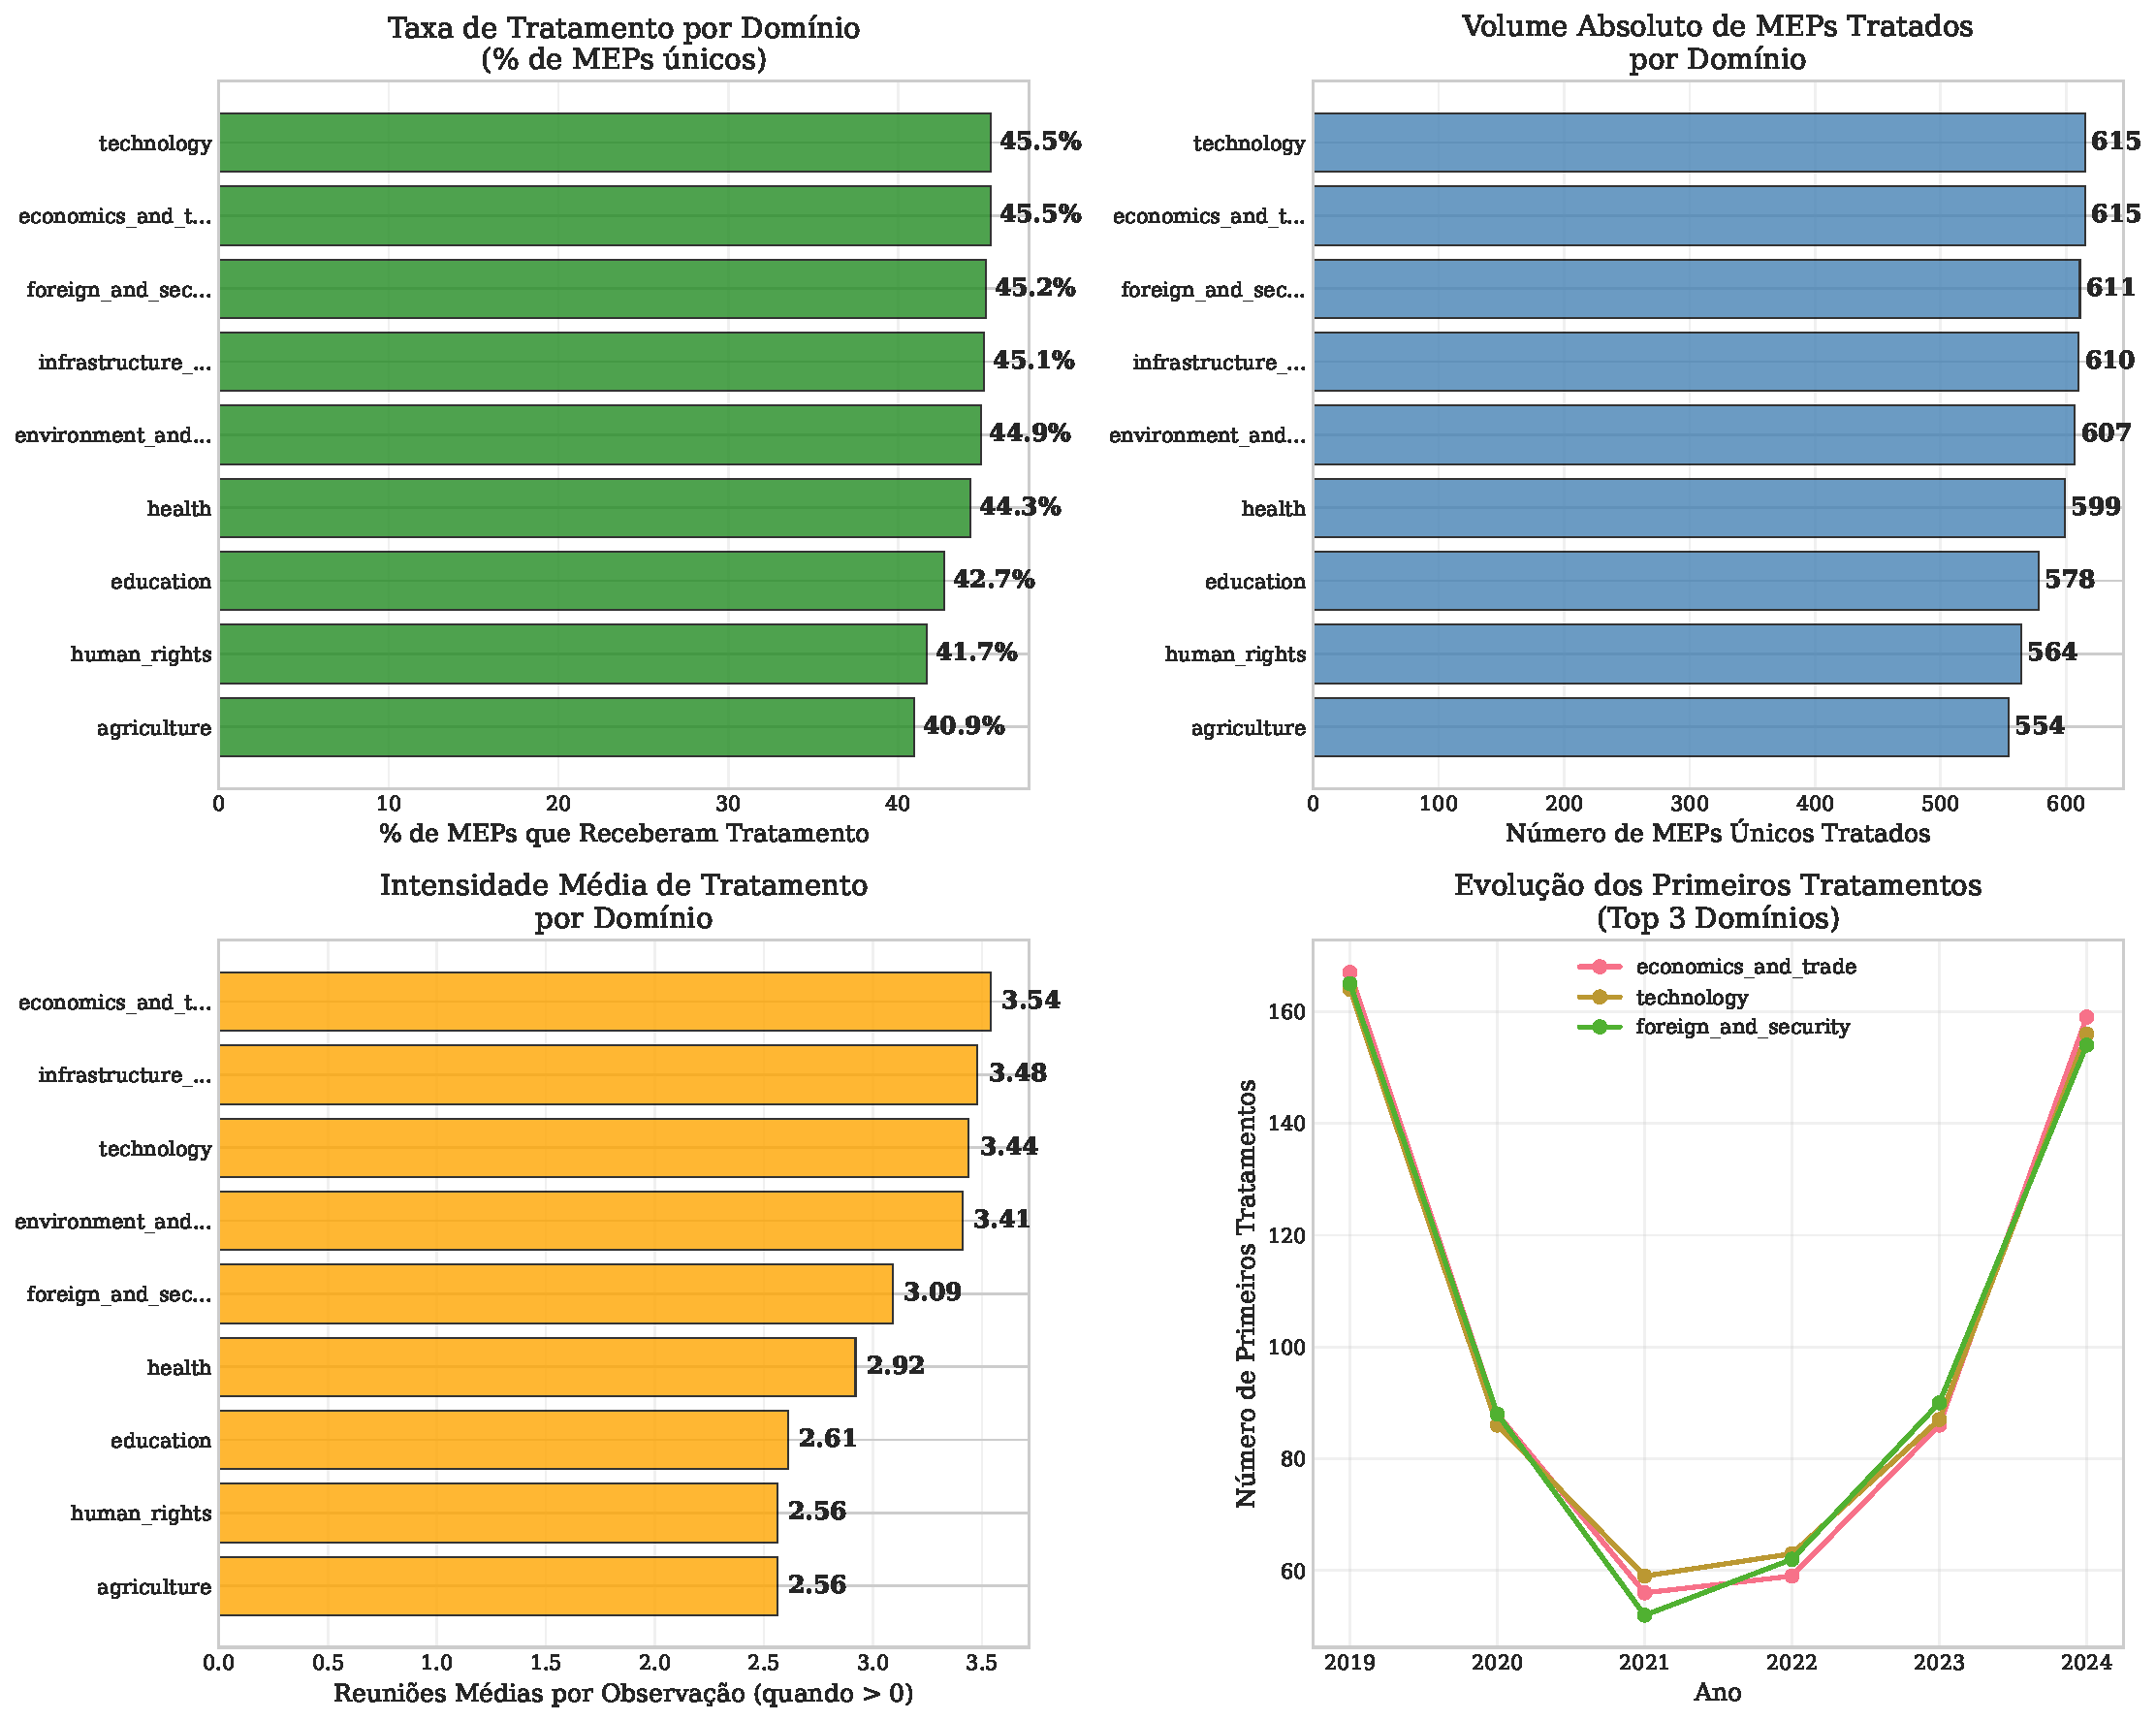
\includegraphics[width=\textwidth]{figures/fig7_domain_treatment_analysis.pdf}
    \caption{Análise detalhada de tratamento por domínio de política pública}
    \label{fig:domain_treatment}
    \note{O painel superior esquerdo mostra a taxa de penetração (percentual de deputados únicos que receberam pelo menos uma reunião em cada domínio). O painel superior direito apresenta o volume absoluto de deputados tratados. O painel inferior esquerdo mostra a intensidade média condicional de tratamento. O painel inferior direito apresenta a evolução temporal dos primeiros tratamentos para os três domínios mais ativos.}
\end{figure}


A heterogeneidade observada entre domínios tem duas implicações metodológicas importantes. Primeiro, a variação sistemática sugere que estimativas de efeito médio podem mascarar diferenças substantivas entre setores, justificando análises de heterogeneidade de efeitos por domínio. Segundo, a ordenação consistente dos domínios por múltiplas métricas (penetração, volume, intensidade) sugere que esta heterogeneidade reflete características estruturais dos setores ao invés de variação aleatória, aumentando a credibilidade de interpretações causais diferenciadas.

% \begin{figure}[htbp]
% \centering
% 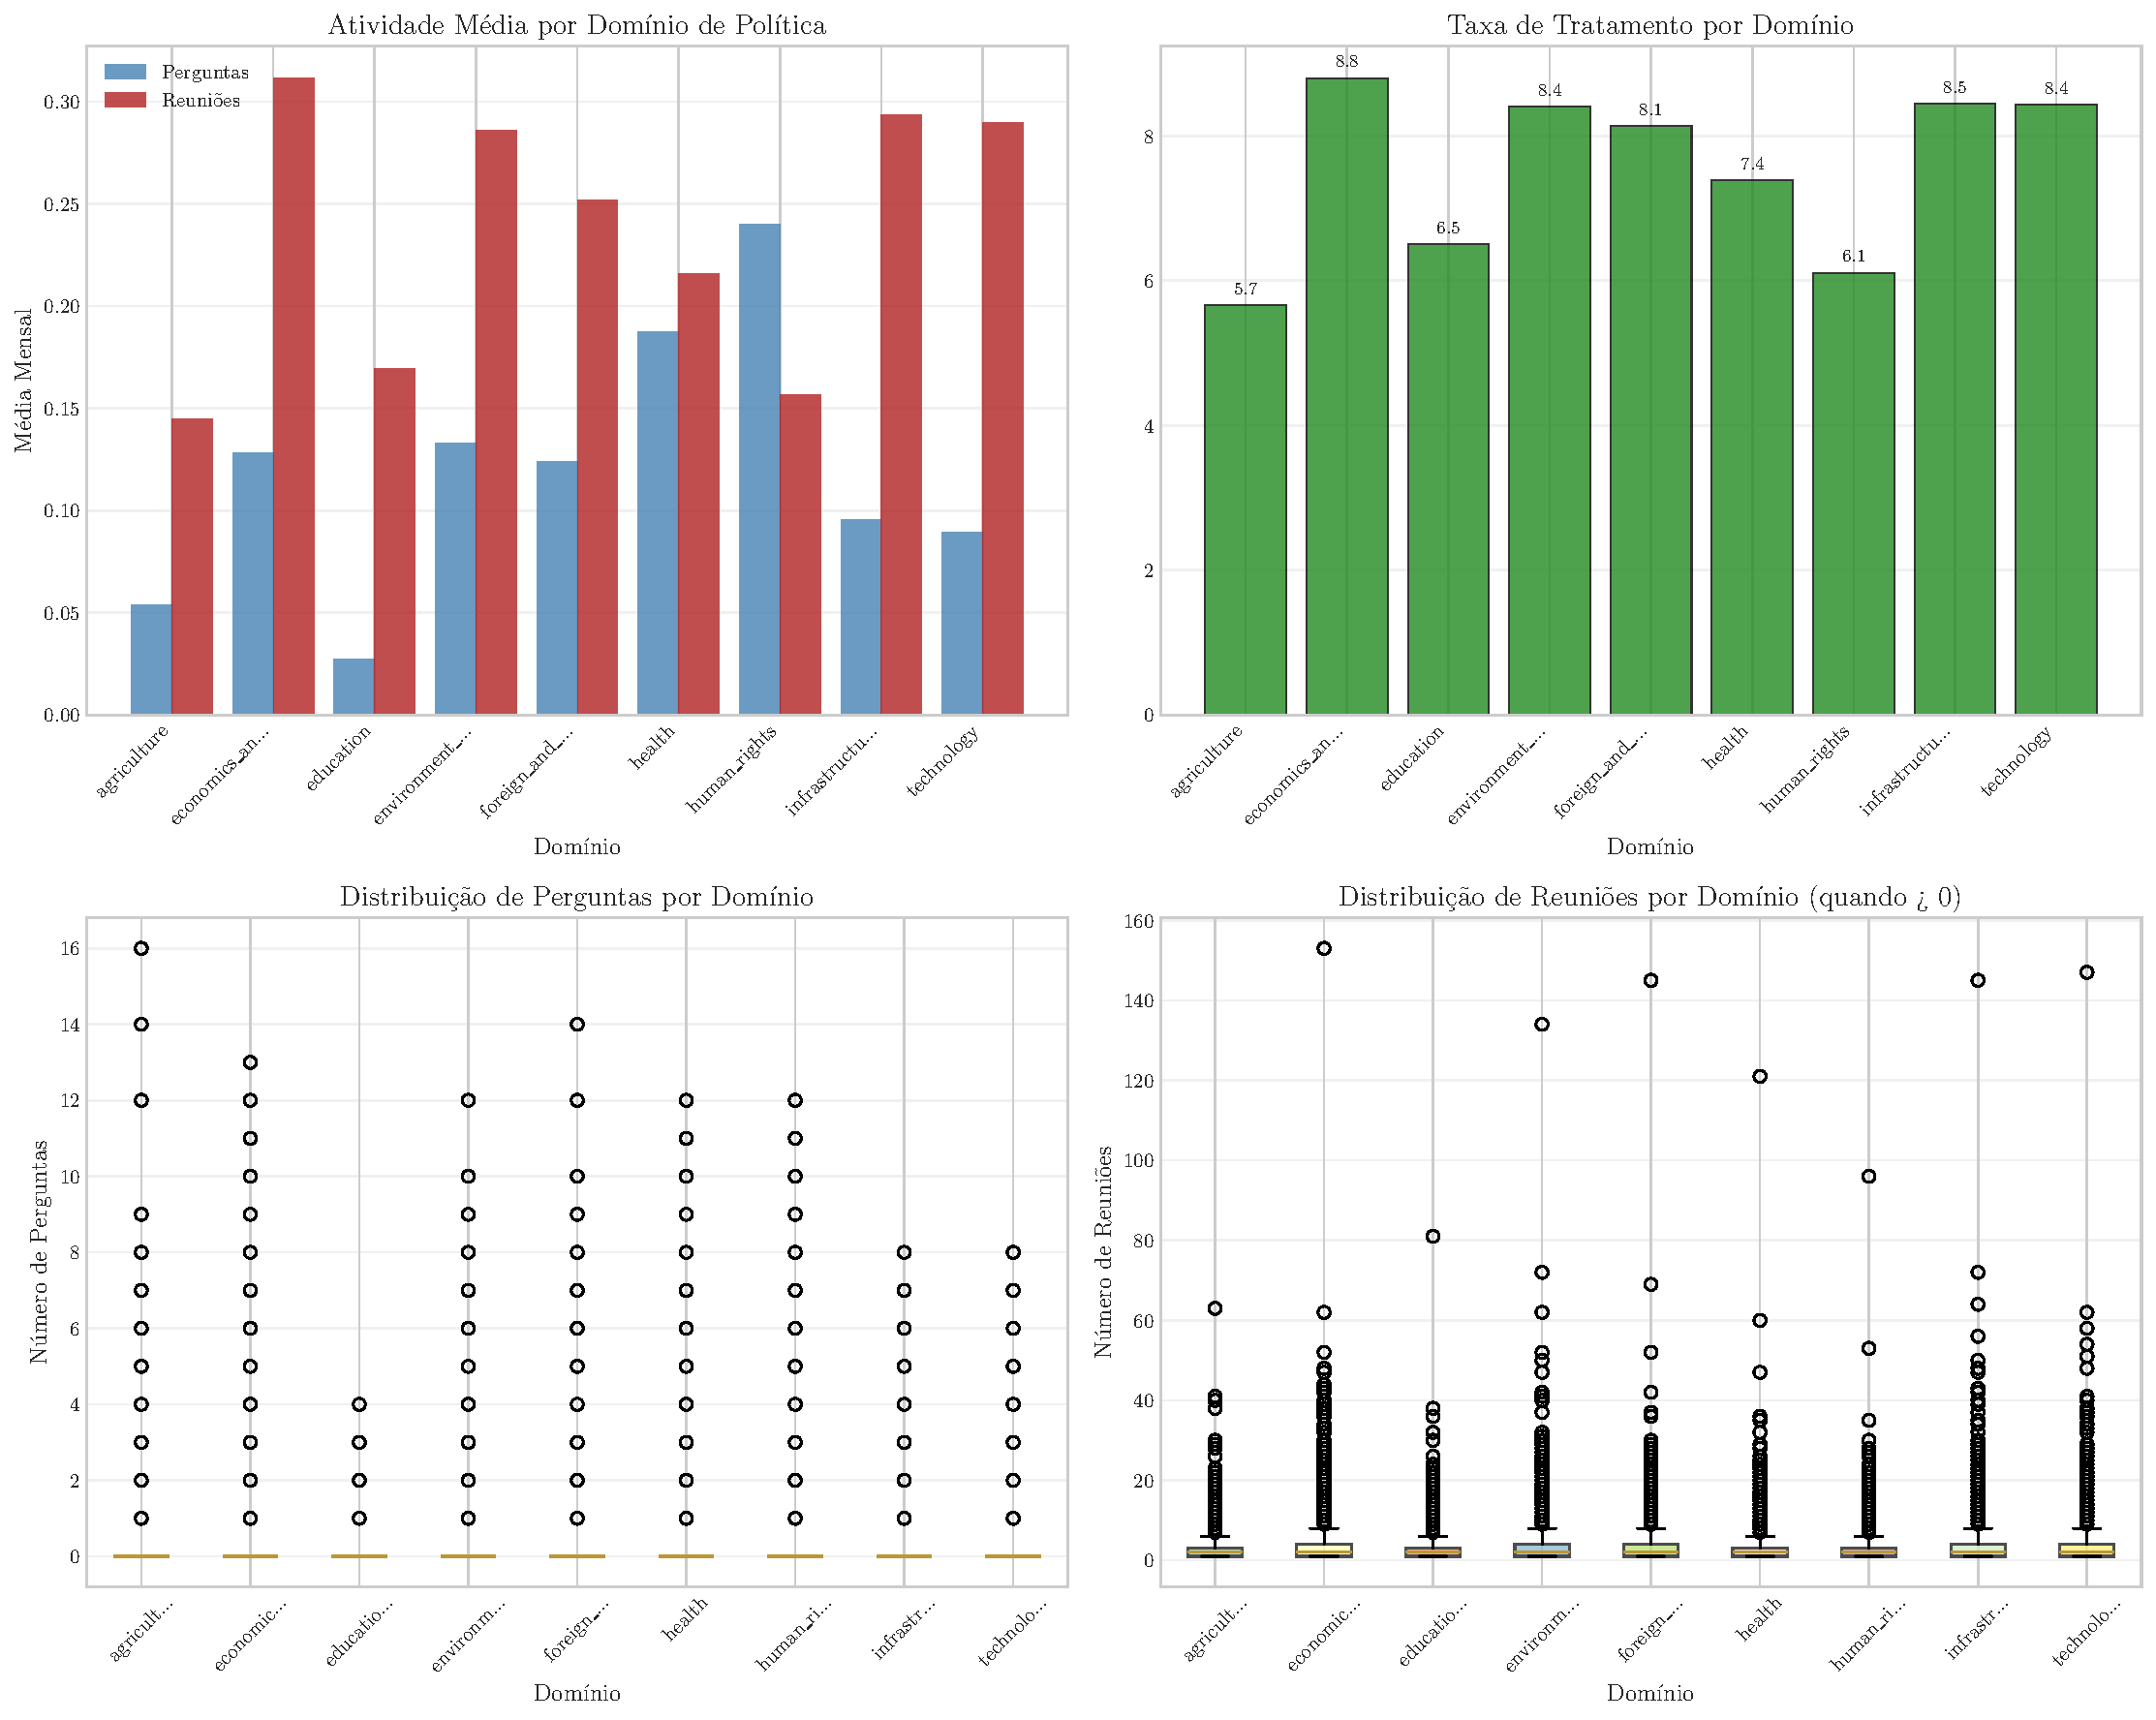
\includegraphics[width=.9\textwidth]{figures/fig3_domain_heterogeneity.pdf}
% \caption{Heterogeneidade por domínio: atividade média e distribuições}
% \label{fig:domain_heterogeneity}
% \note{O painel superior esquerdo mostra a atividade média mensal por domínio para ambas as variáveis. O painel superior direito apresenta as taxas de tratamento mensais. Os painéis inferiores mostram box plots das distribuições completas por domínio, evidenciando tanto diferenças de localização quanto de dispersão entre áreas de política pública.}
% \end{figure}

% \subsection{Análise detalhada: observações MEP-domínio-período}

% Após estabelecer os padrões agregados gerais, temporais e setoriais, esta seção examina as características específicas dos dados no nível mais desagregado: observações MEP-domínio-mês. Esta análise é crucial porque a unidade de observação constitui a base para as estimações econométricas e suas características distribucionais determinam as escolhas metodológicas apropriadas.

% \paragraph{Especialização temática e o problema da inflação artificial de zeros}

A análise da inflação de zeros requer cuidado metodológico particular, pois a unidade de observação MEP-domínio-mês pode gerar inflação \textbf{artificial} de zeros. Como documentado na literatura sobre comportamento parlamentar \cite{example}, deputados tendem a especializar-se tematicamente, concentrando atividade em subconjuntos específicos de domínios. Consequentemente, grupos de interesse, cientes desta especialização, direcionam esforços de lobbying apenas para deputados ativos em suas áreas de interesse.

\textbf{Evidência de especialização temática:} A análise da atividade parlamentar agregada por deputado revela que 97,6\% dos MEPs são \textbf{generalistas} (Índice Herfindahl < 0,4), atuando em média em 7,47 dos 9 domínios disponíveis. Contudo, identificam-se 22 MEPs altamente especializados (HHI > 0,8) que concentram perguntas em domínios únicos, e 26 moderadamente especializados (HHI 0,4-0,8), demonstrando que a especialização, embora limitada, é empiricamente relevante.

\paragraph{Análise corrigida da inflação de zeros}

Para evitar viés na interpretação, a análise da inflação de zeros deve considerar níveis de agregação teoricamente apropriados. A \autoref{tab:zero_inflation_comparison} apresenta uma comparação sistemática entre diferentes níveis de agregação.

\begin{table}[htbp]
\centering
\caption{Inflação de zeros por nível de agregação}
\label{tab:zero_inflation_comparison}
% Usar tabularx para permitir quebra de linha na primeira coluna e evitar overfull hbox
\begin{tabularx}{\textwidth}{>{\raggedright\arraybackslash}X r r r}
\toprule
\textbf{Nível de Agregação} & \textbf{Observações} & \textbf{Zeros Perguntas} & \textbf{Zeros Reuniões} \\
\midrule
MEP-Domínio-Mês (original) & 767{.}151 & 92{,}2\% & 92{,}5\% \\
MEP-Mês (domínios ativos) & 54{.}117 & 70{,}9\% & 85{,}2\% \\
Domínio-Mês (agregado) & 567 & 3{,}2\% & 0{,}0\% \\
\bottomrule
\end{tabularx}
\end{table}

Os resultados revelam que a inflação de zeros é \textbf{sensível ao nível de agregação} e parcialmente \textbf{artificial} quando consideramos especializações temáticas:

\begin{enumerate}
    \item \textbf{Nível MEP-domínio-mês}: A inflação aparentemente extrema (>92\%) reflete em grande parte combinações MEP-domínio onde não se espera atividade sistemática devido à especialização.
    
    \item \textbf{Nível MEP-mês} (agregando apenas domínios onde o MEP demonstra atividade parlamentar): A inflação reduz substancialmente para 70,9\% (perguntas) e 85,2\% (reuniões), revelando que a atividade é \textit{episódica} mas não \textit{ausente}.
    
    \item \textbf{Nível domínio-mês} (agregando todos os MEPs ativos): A inflação torna-se negligível (3,2\% para perguntas, 0\% para reuniões), indicando que há atividade consistente em todos os domínios quando consideramos o conjunto de deputados relevantes.
\end{enumerate}

% A \autoref{fig:corrected_zero_inflation} apresenta uma comparação visual sistemática entre os diferentes níveis de agregação, evidenciando como a especialização temática afeta a interpretação da inflação de zeros.

% \begin{figure}[htbp]
% \centering
% 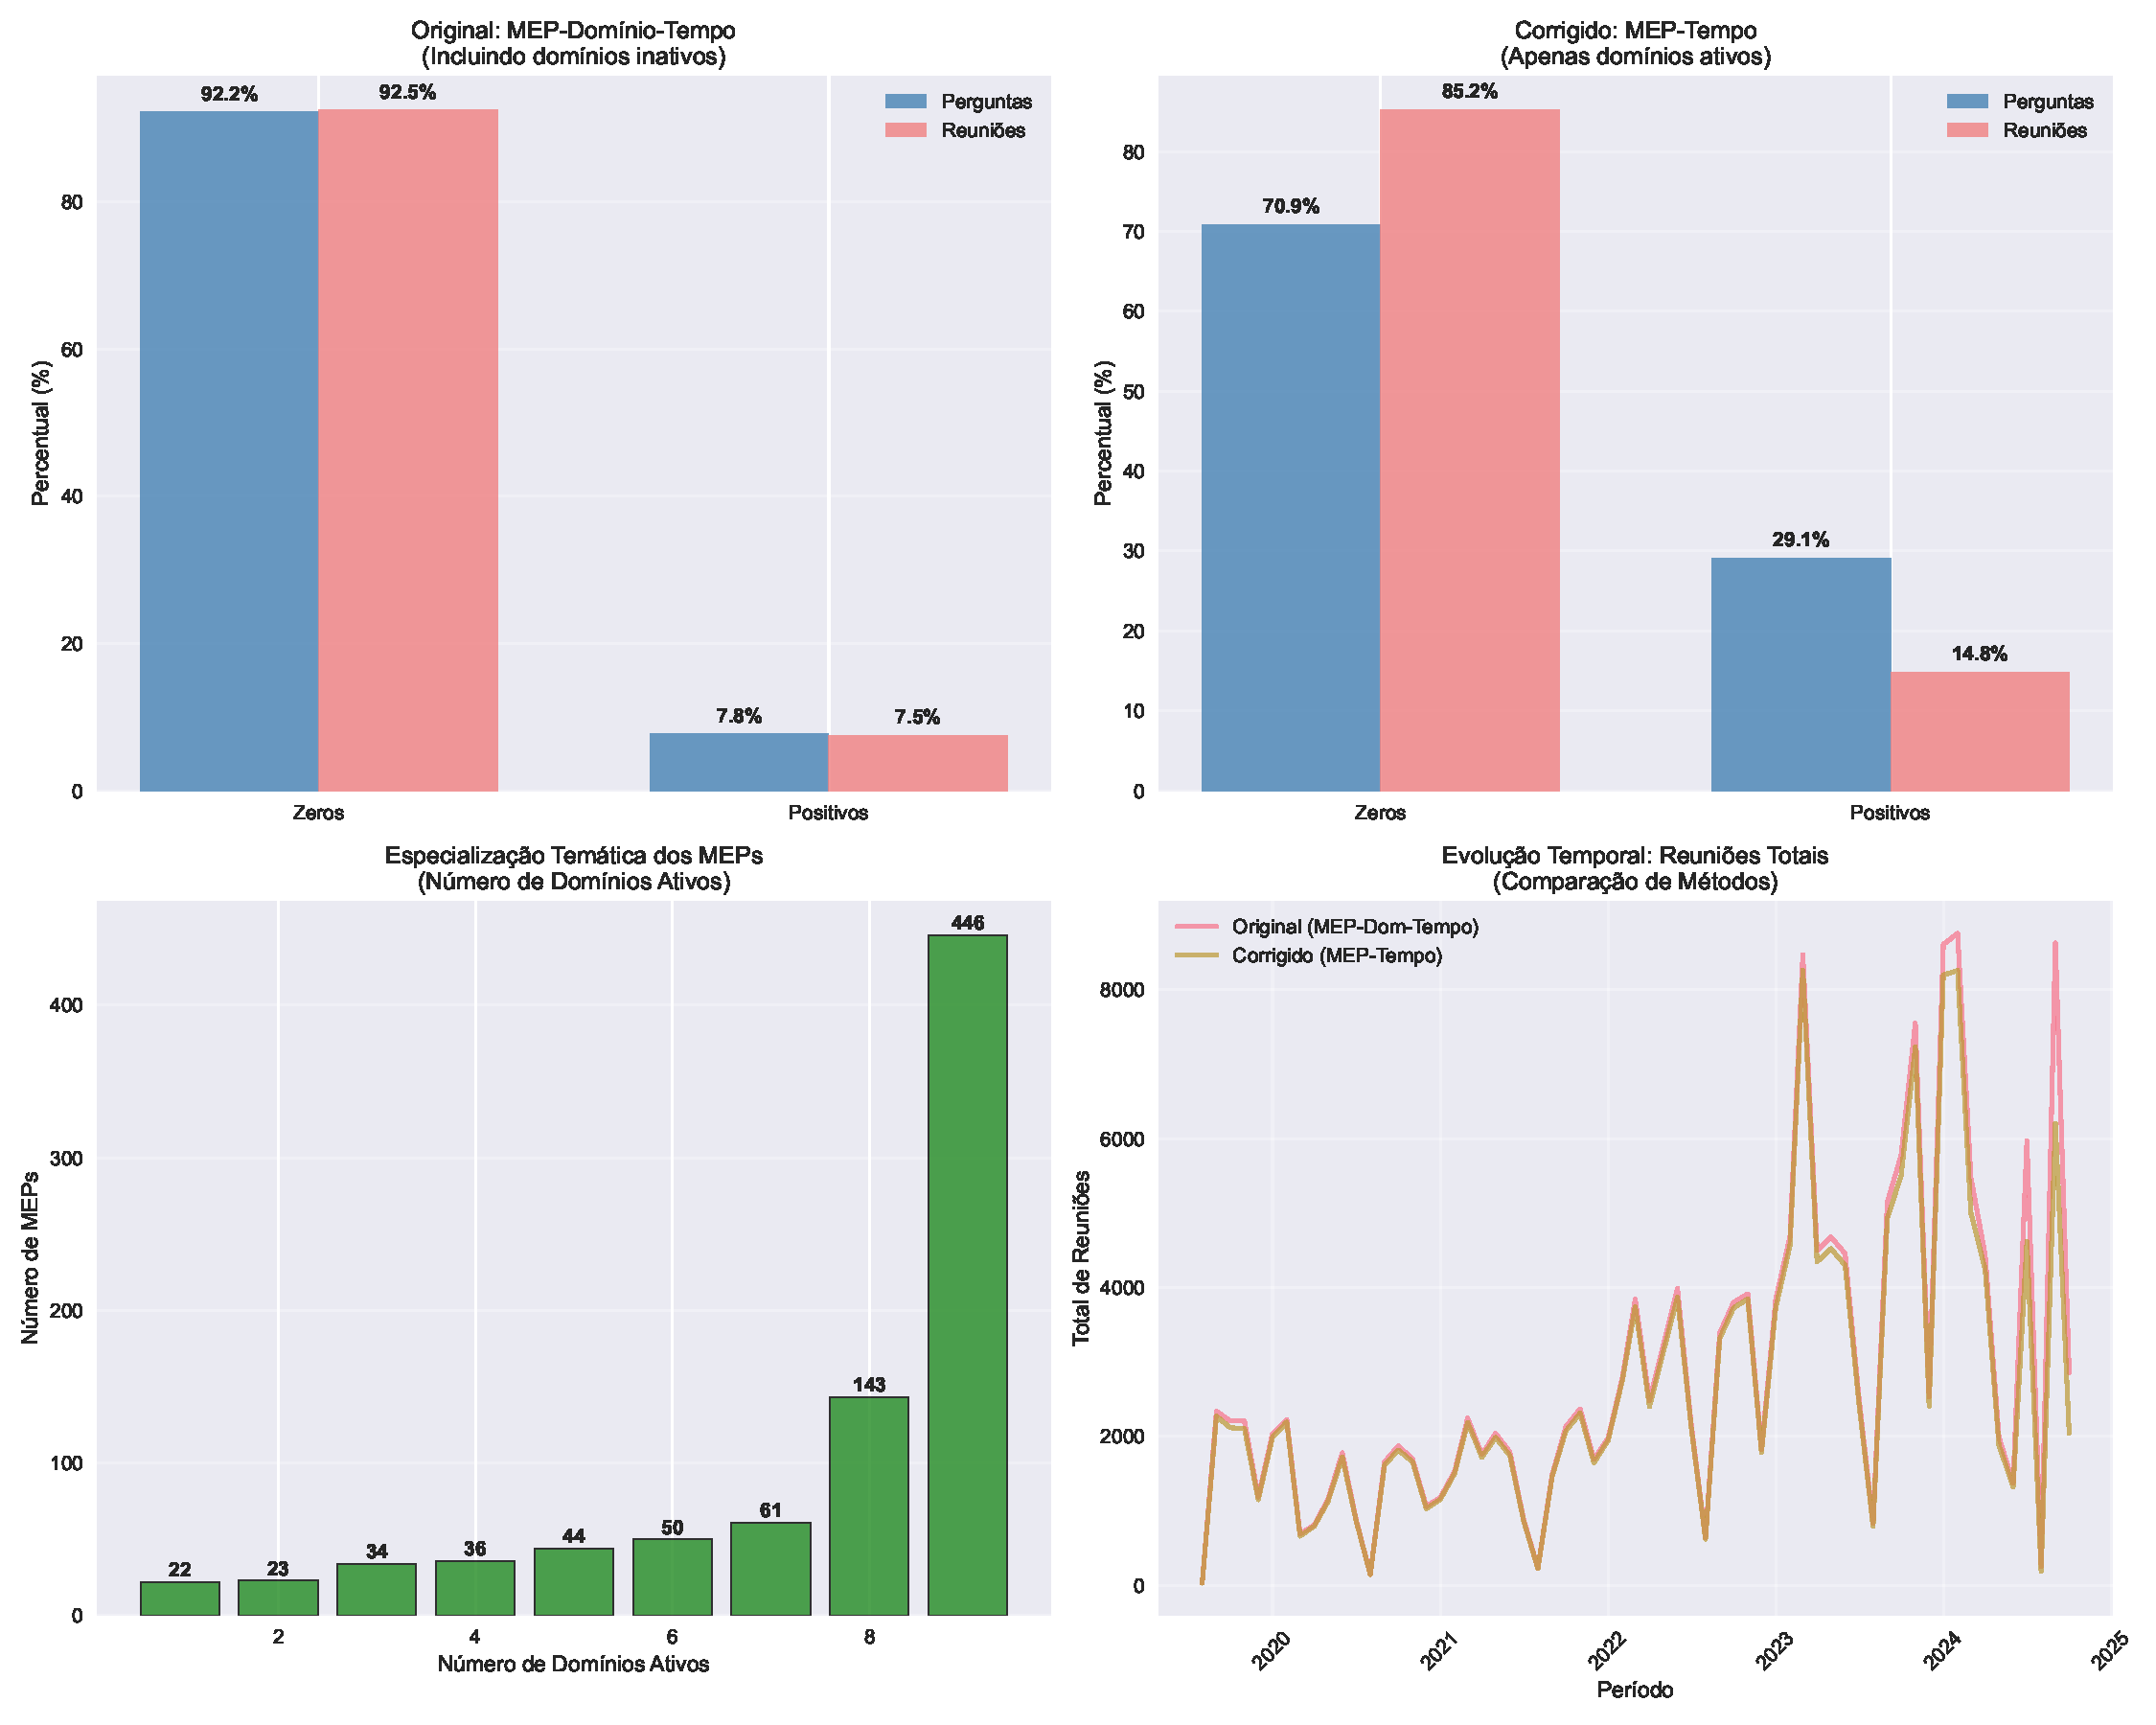
\includegraphics[width=\textwidth]{figures/fig_corrected_zero_inflation_analysis.pdf}
% \caption{Análise corrigida da inflação de zeros considerando especialização temática}
% \label{fig:corrected_zero_inflation}
% \note{O painel superior esquerdo mostra a inflação aparente no nível MEP-domínio-mês original. O painel superior direito apresenta a inflação corrigida no nível MEP-mês considerando apenas domínios ativos. O painel inferior esquerdo mostra a distribuição de especialização temática dos MEPs. O painel inferior direito compara a evolução temporal dos totais mensais entre os métodos original e corrigido.}
% \end{figure}

% \paragraph{Implicações metodológicas revisadas}

Esta análise corrigida tem implicações fundamentais para a estratégia econométrica:

\begin{enumerate}
    \item \textbf{Falso problema de inflação de zeros}: A aparente inflação extrema (>92\%) é em grande parte \textbf{artificial}, resultante da inclusão de combinações MEP-domínio teoricamente implausíveis. A inflação \textbf{real} no nível MEP-mês é substancialmente menor (70,9\%-85,2\%).
    
    \item \textbf{Justificativa para efeitos fixos}: A especialização temática documentada justifica ainda mais fortemente o uso de efeitos fixos MEP×domínio, pois captura heterogeneidade não observada na propensão à atividade em áreas específicas.
    
    \item \textbf{Modelos econométricos apropriados}: Enquanto a inflação moderada (70,9\%) ainda sugere benefícios de modelos de contagem (PPML), a inflação não é tão extrema a ponto de requerer modelos zero-inflated especializados.
    
    \item \textbf{Unidade de análise}: A evidência sustenta a escolha da unidade MEP-domínio-mês para análise causal, pois captura a granularidade necessária para identificação, desde que acompanhada de controles apropriados para especialização.
    
    \item \textbf{Interpretação de resultados}: Efeitos estimados devem ser interpretados condicionalmente à especialização temática, com atenção particular às margens extensiva (entrada em novos domínios) versus intensiva (aumento de atividade em domínios existentes).
\end{enumerate}

% \paragraph{Decomposição em margens extensiva e intensiva}

% A extrema inflação de zeros torna analiticamente vantajoso decompor o fenômeno em duas margens conceituais distintas: a \textbf{margem extensiva} (decisão de participar) e a \textbf{margem intensiva} (nível de atividade condicional à participação). Esta decomposição é teoricamente relevante porque diferentes mecanismos causais podem operar em cada margem.

% A \autoref{fig:extensive_intensive} apresenta uma análise detalhada desta decomposição, incluindo a sobreposição entre atividades parlamentares e de lobbying.

% \begin{figure}[htbp]
% \centering
% 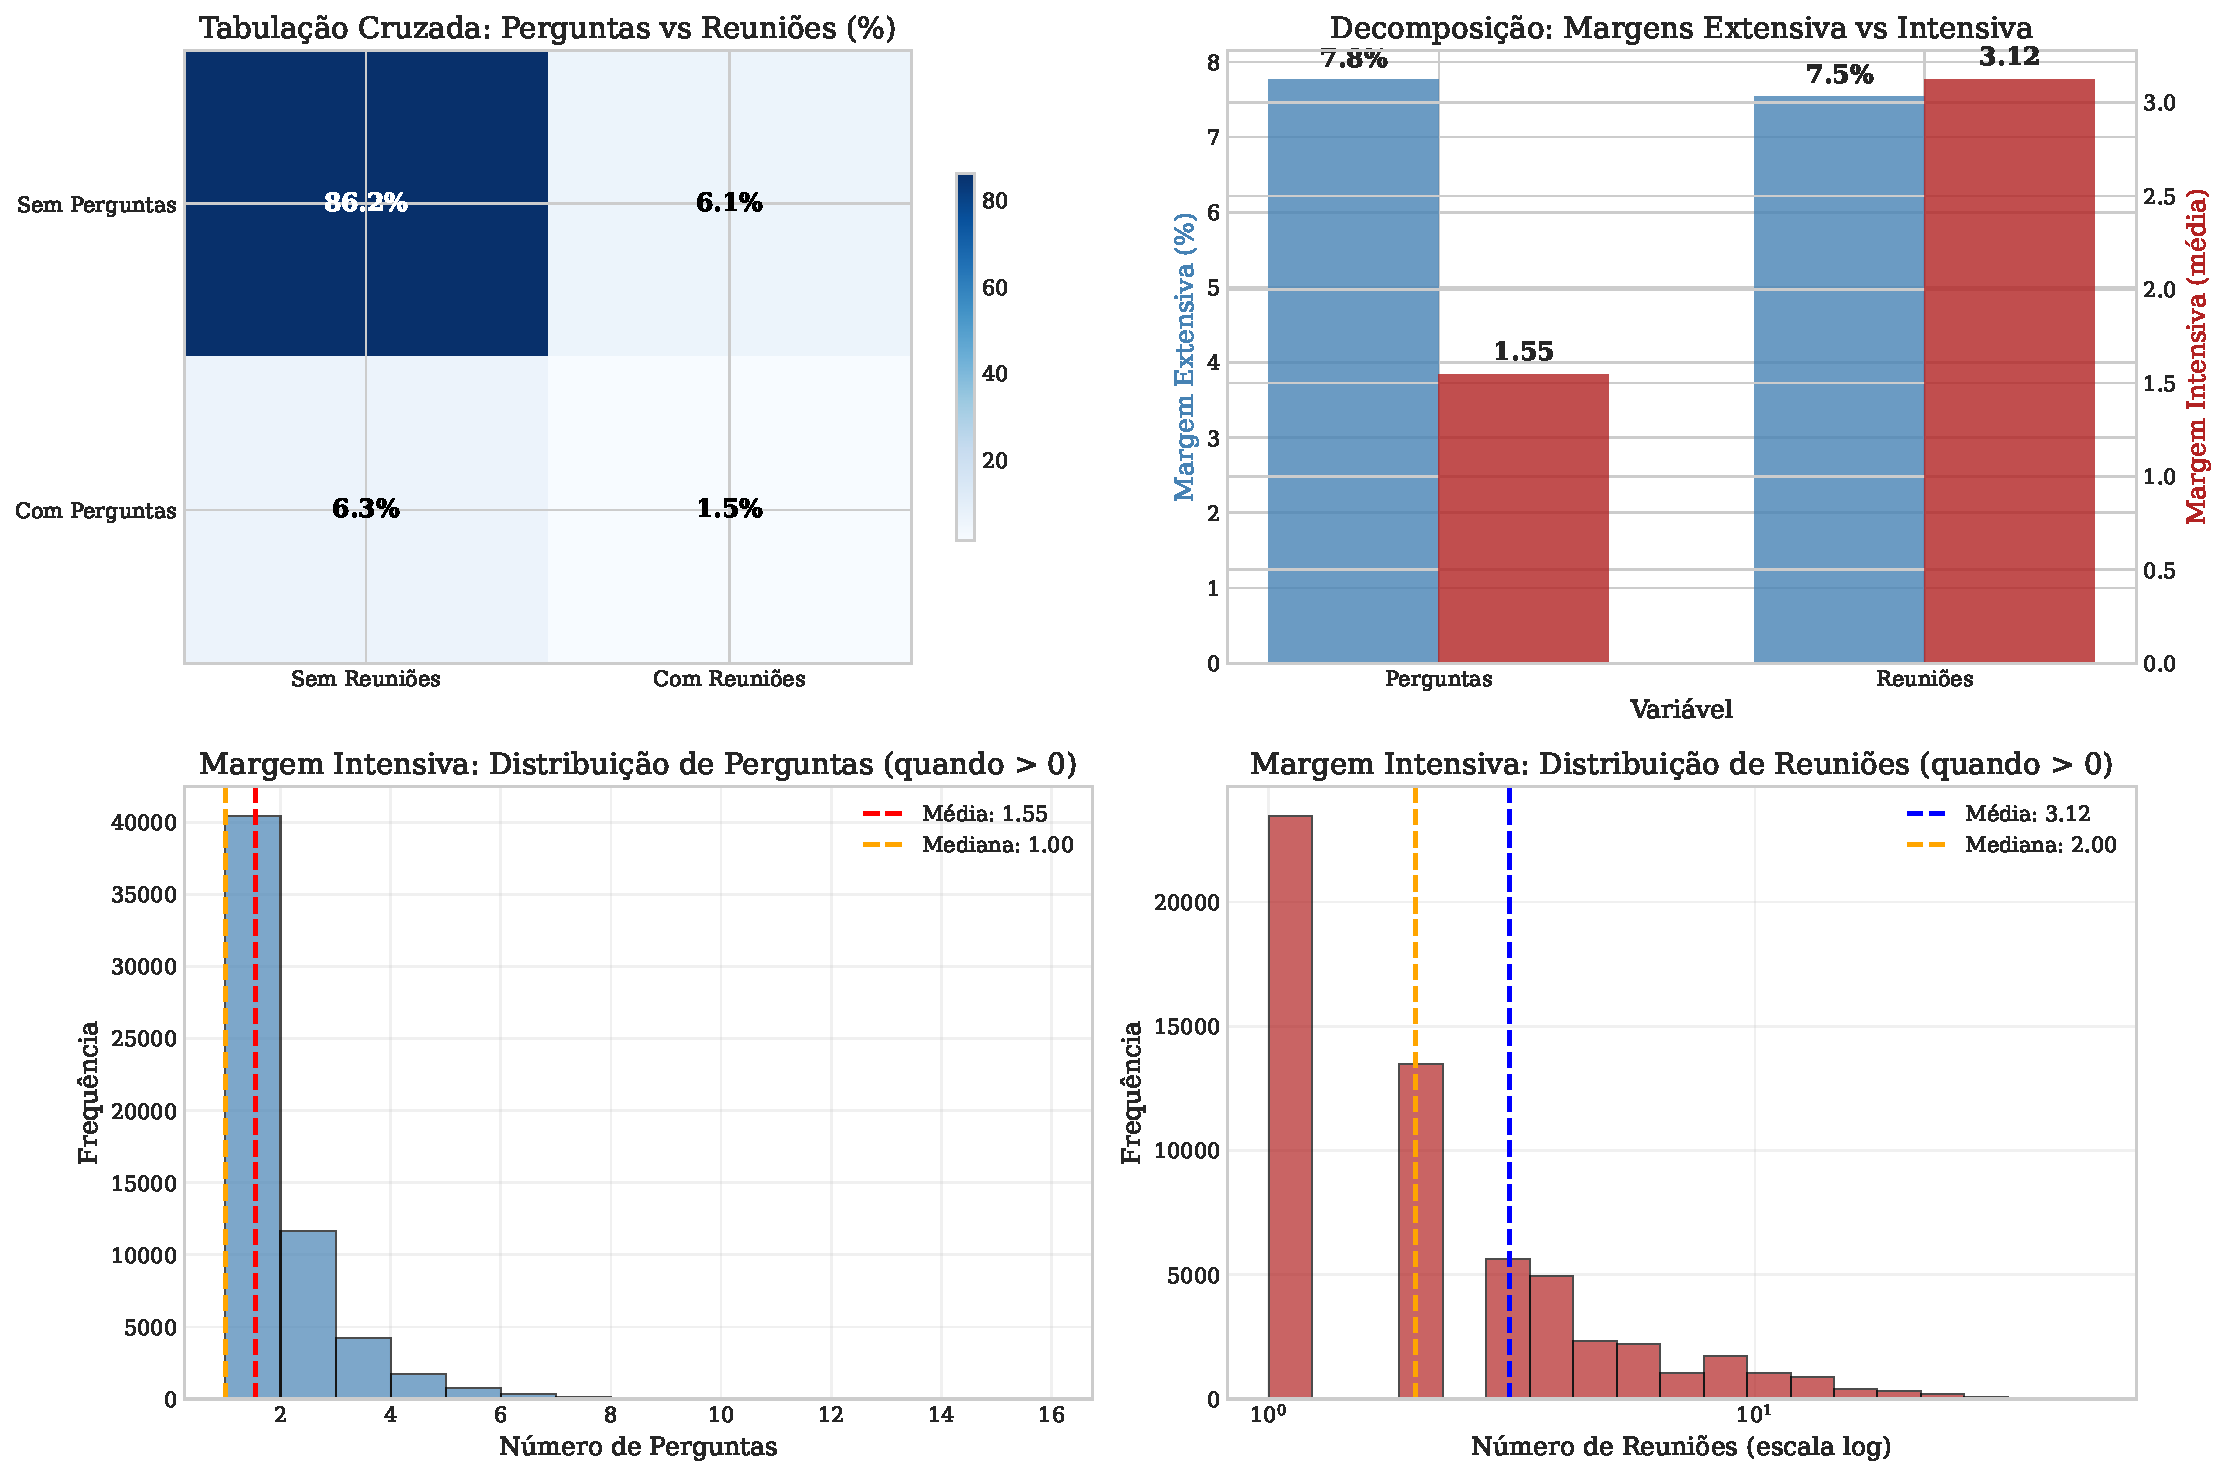
\includegraphics[width=\textwidth]{figures/fig5_extensive_intensive_margins.pdf}
% \caption{Análise das margens extensiva e intensiva}
% \label{fig:extensive_intensive}
% \note{O painel superior esquerdo apresenta a tabulação cruzada entre atividade parlamentar e de lobbying, revelando padrões de sobreposição. O painel superior direito decompõe as margens extensiva (participação) e intensiva (intensidade condicional). Os painéis inferiores mostram as distribuições condicionais completas para ambas as variáveis na margem intensiva.}
% \end{figure}

% A tabulação cruzada revela um padrão notável: apenas \textbf{0,4\%} das observações apresentam simultaneamente perguntas parlamentares e reuniões de lobbying. Esta baixa sobreposição indica que atividade parlamentar e lobbying são largamente \textbf{independentes} no nível temporal mensal, sugerindo que potenciais efeitos causais podem operar através de canais indiretos ou com defasagens temporais que não são captadas na correlação contemporânea.

% Na margem extensiva, 7,8\% das observações apresentam atividade parlamentar e 7,5\% apresentam atividade de lobbying. Na margem intensiva, condicionalmente à participação, as médias são 1,54 perguntas e 3,15 reuniões por observação, com distribuições altamente assimétricas evidenciando concentração mesmo dentro do subconjunto de observações ativas.

% \paragraph{Correlações e relações entre variáveis}

% Para completar a caracterização dos dados, a \autoref{fig:correlation_analysis} examina as relações diretas entre as variáveis principais através de múltiplas perspectivas analíticas.

% \begin{figure}[htbp]
% \centering
% 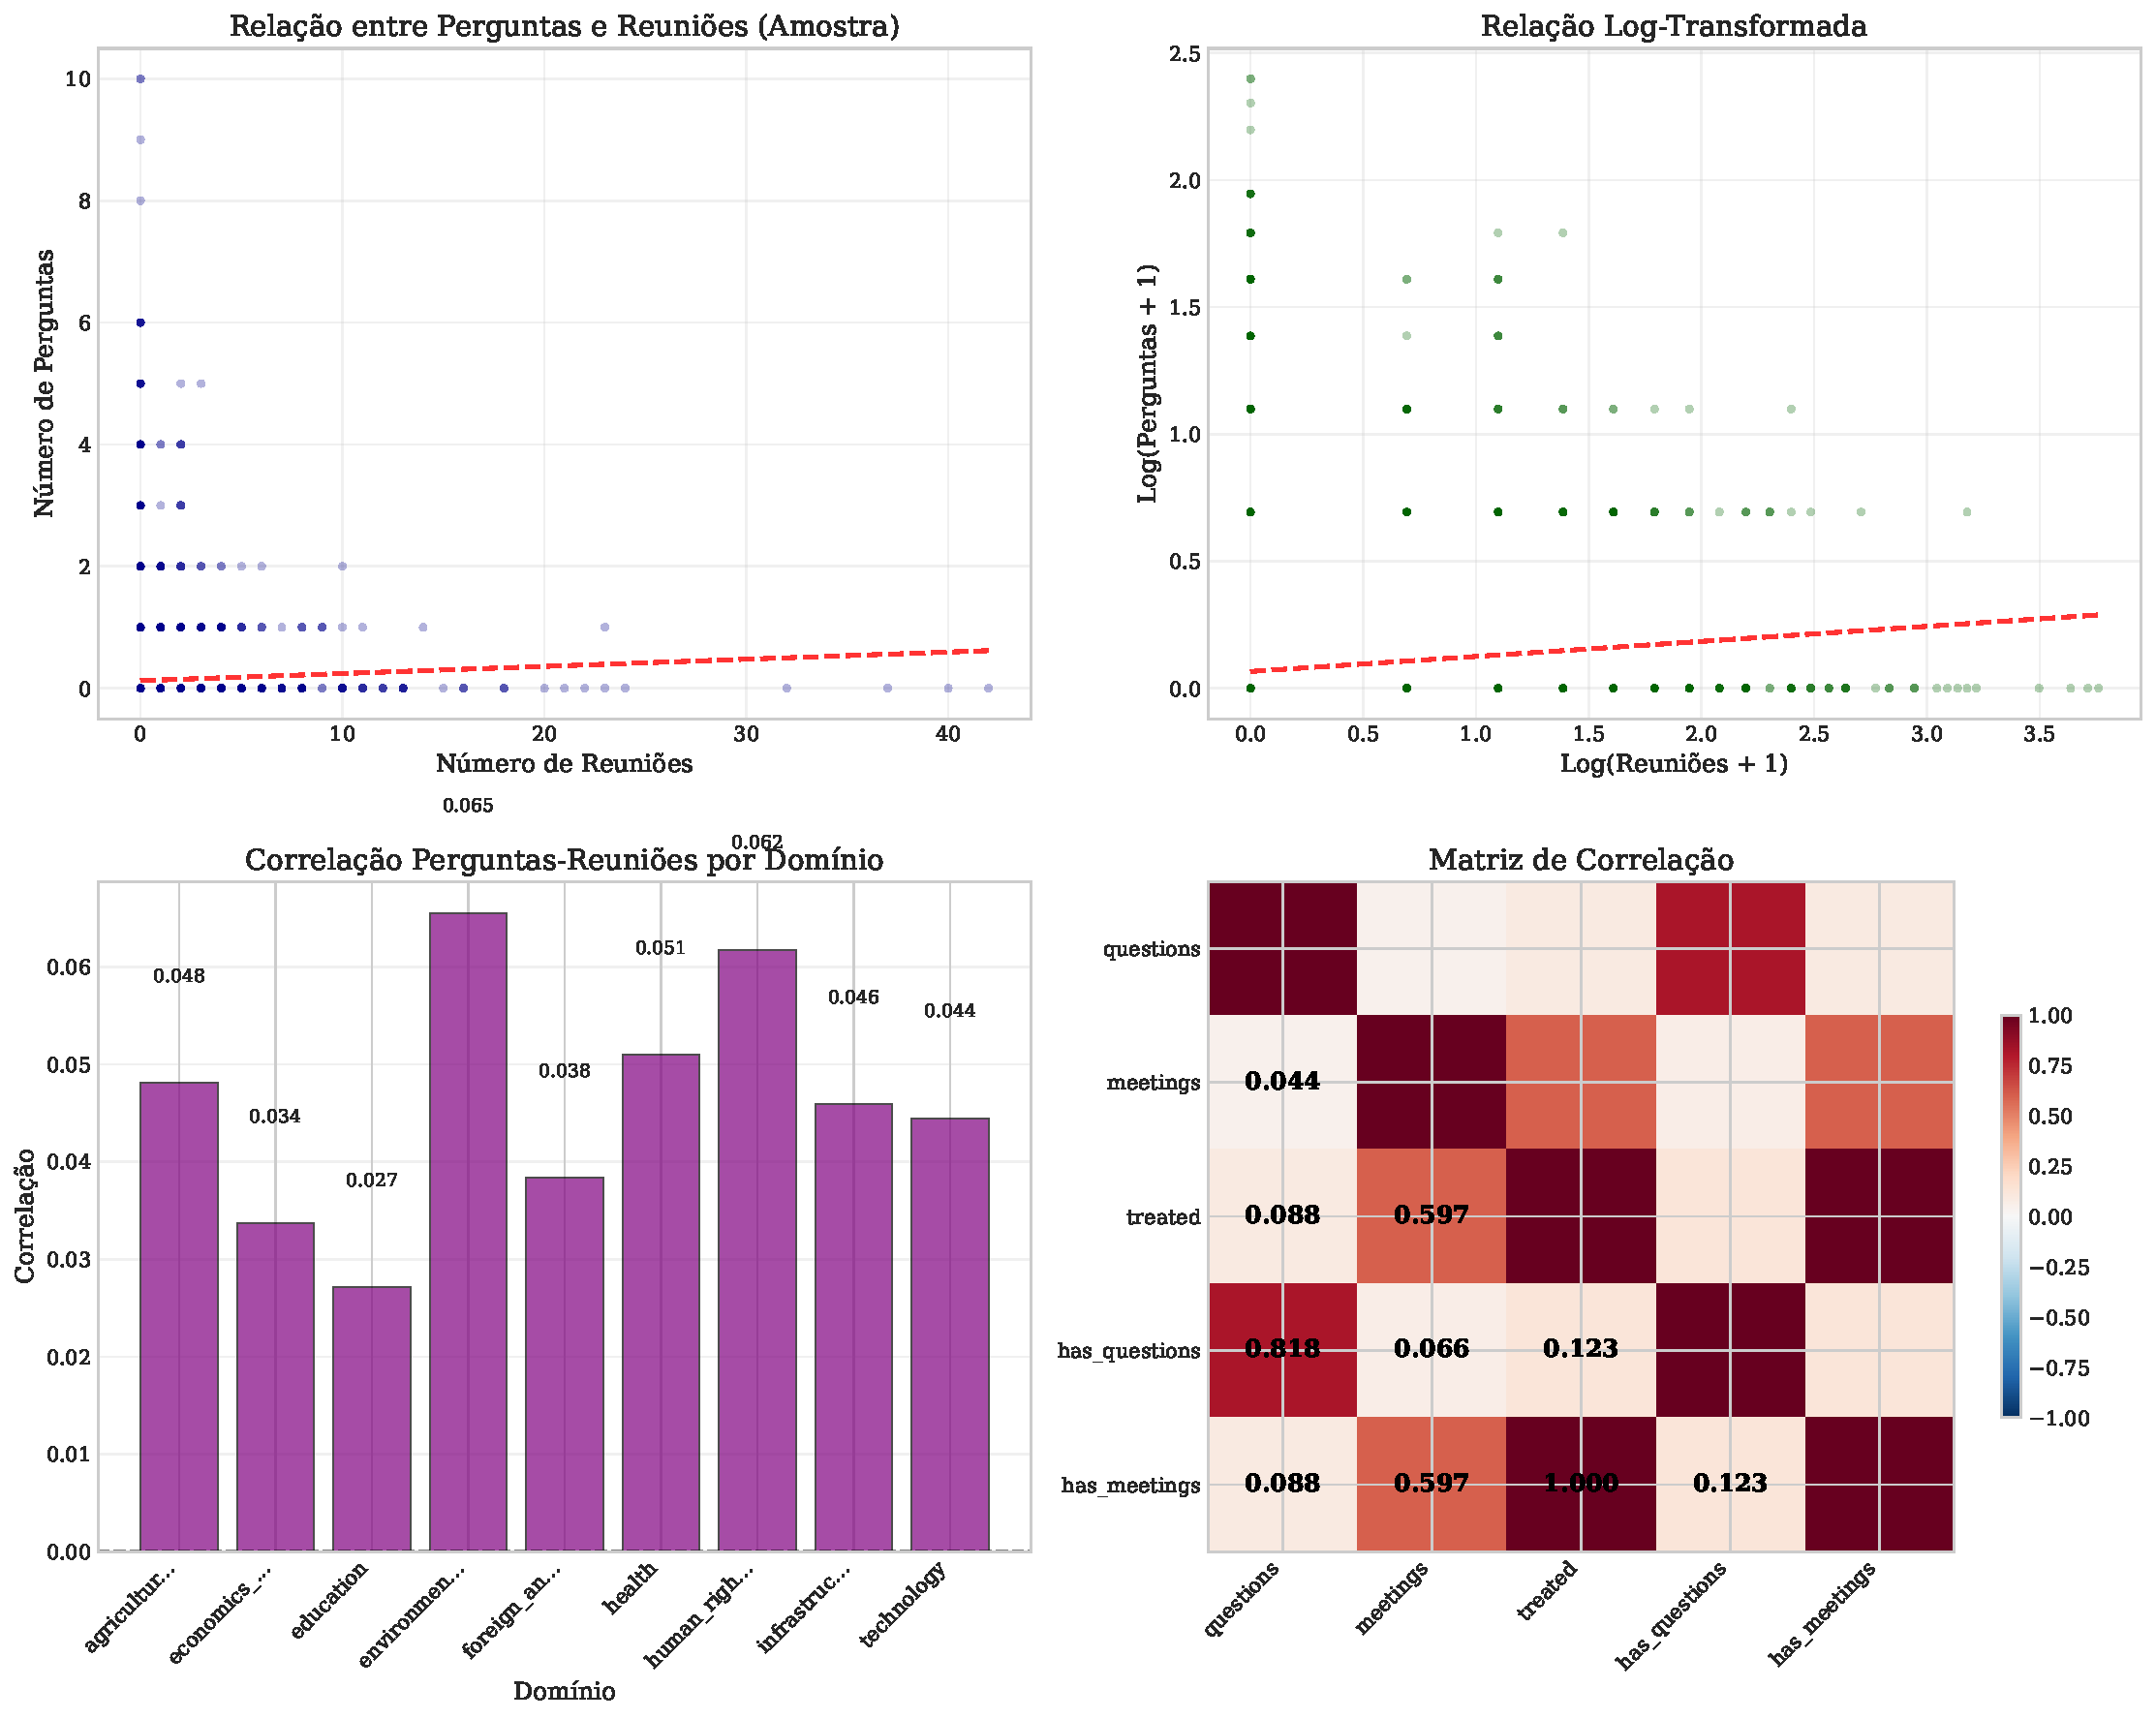
\includegraphics[width=\textwidth]{figures/fig4_correlation_analysis.pdf}
% \caption{Análise de correlações e relações entre variáveis}
% \label{fig:correlation_analysis}
% \note{O painel superior esquerdo mostra a relação geral entre perguntas e reuniões no nível MEP-domínio-mês. O painel superior direito apresenta a mesma relação em escala logarítmica. O painel inferior esquerdo mostra as correlações por domínio. O painel inferior direito apresenta a matriz de correlação entre as variáveis principais.}
% \end{figure}

% A análise de correlações revela padrões consistentes com a baixa sobreposição contemporânea observada anteriormente. No nível agregado MEP-domínio-mês, a correlação é positiva mas modesta. Interessantemente, existe heterogeneidade sistemática nas correlações entre domínios, sugerindo que a força da relação varia com características setoriais específicas.

\subsection{Síntese e implicações metodológicas}

A análise descritiva multinível revela um conjunto coerente de \textit{stylized facts} que informam tanto a compreensão teórica quanto as escolhas metodológicas para a análise causal subsequente.

% \paragraph{Características empíricas principais}

Primeiro, o \textbf{lobbying é um fenômeno disseminado mas episódico}. Enquanto 46,3\% dos deputados recebem lobbying durante o período estudado, a atividade temporal é concentrada: considerando apenas domínios onde MEPs demonstram atividade parlamentar, 70,9\% das observações MEP-mês não apresentam perguntas e 85,2\% não apresentam reuniões, indicando que a influência opera através de interações concentradas temporalmente.

Segundo, existe \textbf{concentração extrema} em múltiplas dimensões. No nível individual, a distribuição de reuniões é altamente assimétrica (mediana 105, média 288, máximo 4.274). Crucialmente, a aparente inflação extrema de zeros (>92\%) no nível MEP-domínio-mês é em grande parte artificial, refletindo combinações onde não se espera atividade devido à especialização temática.

Terceiro, observa-se \textbf{heterogeneidade sistemática entre domínios} em todas as métricas analisadas. Domínios de regulação econômica apresentam consistentemente maior atividade de lobbying, refletindo diferenças estruturais em stakes econômicos e capacidade organizacional. Esta heterogeneidade é consistente com a especialização temática documentada.

Quarto, a \textbf{especialização temática é limitada mas empiricamente relevante}: enquanto 97,6\% dos MEPs atuam como generalistas (HHI < 0,4), existem 22 deputados altamente especializados e 26 moderadamente especializados, com padrões claros de concentração que informam estratégias de lobbying e justificam controles econométricos específicos.

Quinto, a \textbf{correlação contemporânea entre lobbying e atividade parlamentar é baixa} no nível temporal mensal, mas padrões agregados sugerem relações mais complexas que podem envolver defasagens temporais ou mecanismos indiretos.

% \paragraph{Implicações para estratégia econométrica}

Estas características empíricas têm implicações diretas para a escolha da estratégia econométrica:

\begin{enumerate}
    \item \textbf{Especificação funcional}: A inflação moderada de zeros (70,9\%-85,2\% após correção) e natureza de contagem das variáveis justificam o uso de estimadores Poisson Pseudo-Maximum Likelihood (PPML), mas não requerem modelos zero-inflated especializados.
    
    \item \textbf{Estrutura de efeitos fixos}: A evidência de especialização temática justifica fortemente efeitos fixos MEP×domínio para controlar heterogeneidade não observada na propensão à atividade em áreas específicas, complementados por efeitos fixos temporais.
    
    \item \textbf{Correção de viés de seleção}: A especialização temática implica que observações MEP-domínio-mês com probabilidade zero de atividade podem distorcer estimativas. Controles ou exclusões baseadas em atividade histórica podem ser apropriados.
    
    \item \textbf{Estrutura de erros}: A concentração temporal da atividade e especialização justificam erros-padrão agrupados no nível MEP×domínio para capturar correlação serial específica por área de atuação.
    
    \item \textbf{Análise de heterogeneidade}: A variação sistemática entre domínios, combinada com especialização, justifica análises diferenciadas por setor e investigação de efeitos nas margens extensiva (entrada em novos domínios) versus intensiva.
    
    \item \textbf{Interpretação causal}: Efeitos estimados devem ser interpretados condicionalmente à especialização temática existente, distinguindo entre expansão de atividade em domínios familiares versus diversificação para novas áreas.
\end{enumerate}

Finalmente, a \textbf{estrutura balanceada do painel} e a \textbf{cobertura temporal substancial} fornecem condições ideais para estratégias de identificação baseadas em variação temporal within-individual, maximizando o poder estatístico while minimizando preocupações com confounding não observado time-invariant.

Esta análise descritiva abrangente estabelece as bases empíricas sólidas para a estratégia de identificação causal apresentada na seção seguinte, demonstrando que os dados possuem as características necessárias para investigar rigorosamente os efeitos do lobbying na atividade parlamentar dos deputados europeus.

% !TeX root = ../../main.tex
\section{Análise de efeitos do lobby}
\label{sec:resultados_efeitos}

Optamos por estimar modelos de contagem via \acrshort{ppml} com \textit{link} logaritmo por três razões principais. Primeiro, as variáveis de interesse (perguntas e reuniões) são contagens, com forte assimetria e alta incidência de zeros no nível MEP–domínio–mês. O \acrshort{ppml} lida naturalmente com zeros sem exigir transformações logarítmicas \textit{ad hoc} que descartam observações. Segundo, o \acrshort{ppml} é consistente sob especificação correta da média condicional mesmo na presença de sobredispersão e heterocedasticidade não especificada, fornecendo erros-padrão robustos quando combinados com \textit{clustering}. Terceiro, a implementação com efeitos fixos de alta dimensão é estável e amplamente utilizada na literatura aplicada (estimador \texttt{fepois} do pacote \texttt{fixest}).

No \acrshort{ppml} com \textit{link} log, a expectativa condicional é \(\mathbb{E}[y\mid X] = \exp(X\beta)\). Assim, para um regressor contínuo \(x_k\) (por exemplo, \textit{meetings} em nível), o coeficiente \(\beta_k\) tem interpretação multiplicativa: um aumento de uma unidade em \(x_k\) está associado a uma variação percentual de \(100\times(\mathrm{e}^{\beta_k}-1)\%\) na média de \(y\), \textit{ceteris paribus}.

A especificação segue o \textit{framework} analítico delineado no capítulo: controlamos por heterogeneidade não observada ao nível do membro e por choques comuns estruturados por partido, país e domínio ao longo do tempo. Concretamente, estimamos modelos com efeitos fixos de membro (\texttt{member\_id}) e efeitos fixos tempo-variantes por país (\texttt{country\_time}), por partido (\texttt{party\_time}) e por domínio (\texttt{domain\_time}). Os erros-padrão são agrupados em \textit{domínio×tempo} e \textit{membro}, capturando correlação serial e choques idiossincráticos nesse nível, conforme implementado nos scripts empíricos.

Essa modelagem garante três propriedades fundamentais para a identificação dos efeitos: (i) permite comparar a evolução da atividade do mesmo \acrshort{mpe} ao longo do tempo, controlando por características não observadas e invariantes como preferências individuais, capital político e produtividade; (ii) elimina a influência de choques ou tendências comuns a todos os \acrshort{mpe}s de um mesmo país ou partido em cada mês, por meio dos efeitos fixos específicos de país$\times$tempo e partido$\times$tempo; e (iii) assegura robustez frente a choques específicos de cada setor ou área temática ao incorporar efeitos fixos de domínio$\times$tempo (\texttt{domain\_time}), isolando variações idiossincráticas desses contextos.

Para testar a Hipótese 1, utilizamos o painel agregado MEP–domínio–mês em amostra combinada (\textit{pooled}) e estimamos PPML com a estrutura de efeitos fixos descrita acima. O coeficiente associado às reuniões (\textit{meetings}) é \textbf{positivo}, indicando que aumentos na intensidade de lobbying estão associados a maior atividade parlamentar em termos de perguntas. Esse resultado é consistente em especificações alternativas, incluindo a versão com termo quadrático para capturar possíveis não linearidades e a inclusão de efeitos fixos \textit{domínio×tempo}, sugerindo robustez do sinal e da magnitude qualitativa do efeito.

Em termos de interpretação, mantidos constantes os efeitos fixos, um incremento marginal em reuniões está associado a um aumento proporcional na média de perguntas dado por \(\mathrm{e}^{\hat{\beta}}-1\). Reportamos os efeitos como variações percentuais estimadas na seção de tabelas de resultados, com intervalos de confiança baseados em erros-padrão agrupados.

\begin{table}[htbp]
\centering
\caption{Resumo dos modelos \acrshort{ppml} para a Hipótese 1}
\label{tab:ppml_h1_both}
\begin{tabularx}{\textwidth}{>{\raggedright\arraybackslash}p{.22\textwidth} >{\raggedright\arraybackslash}X >{\raggedright\arraybackslash}X}
\toprule
  & PPML & PPML (Quad.) \\
\midrule
Reuni\~oes & 0.013*** (0.002) & 0.037*** (0.005) \\
Reuni\~oes$^2$ &  & -0.001*** (0.000) \\
\midrule
Observa\c{c}\~oes & 711,855 & 711,855 \\
Efeitos fixos & \multicolumn{2}{p{.72\textwidth}}{\raggedright pa\'is$\times$tempo; partido$\times$tempo; dom\'inio$\times$tempo} \\
Cluster & \multicolumn{2}{p{.72\textwidth}}{\raggedright dom\'inio$\times$tempo; membro} \\
\bottomrule
\end{tabularx}

\note{A coluna ``PPML'' reporta o modelo principal com efeito linear em \textit{meetings}. A coluna ``PPML (Quadrático)'' adiciona \(\textit{meetings}^2\) para capturar retornos marginais decrescentes. Efeitos fixos: membro; país$\times$tempo; partido$\times$tempo. Erros-padrão agrupados em domínio$\times$tempo e membro.}
\end{table}

\begin{figure}[htbp]
\centering
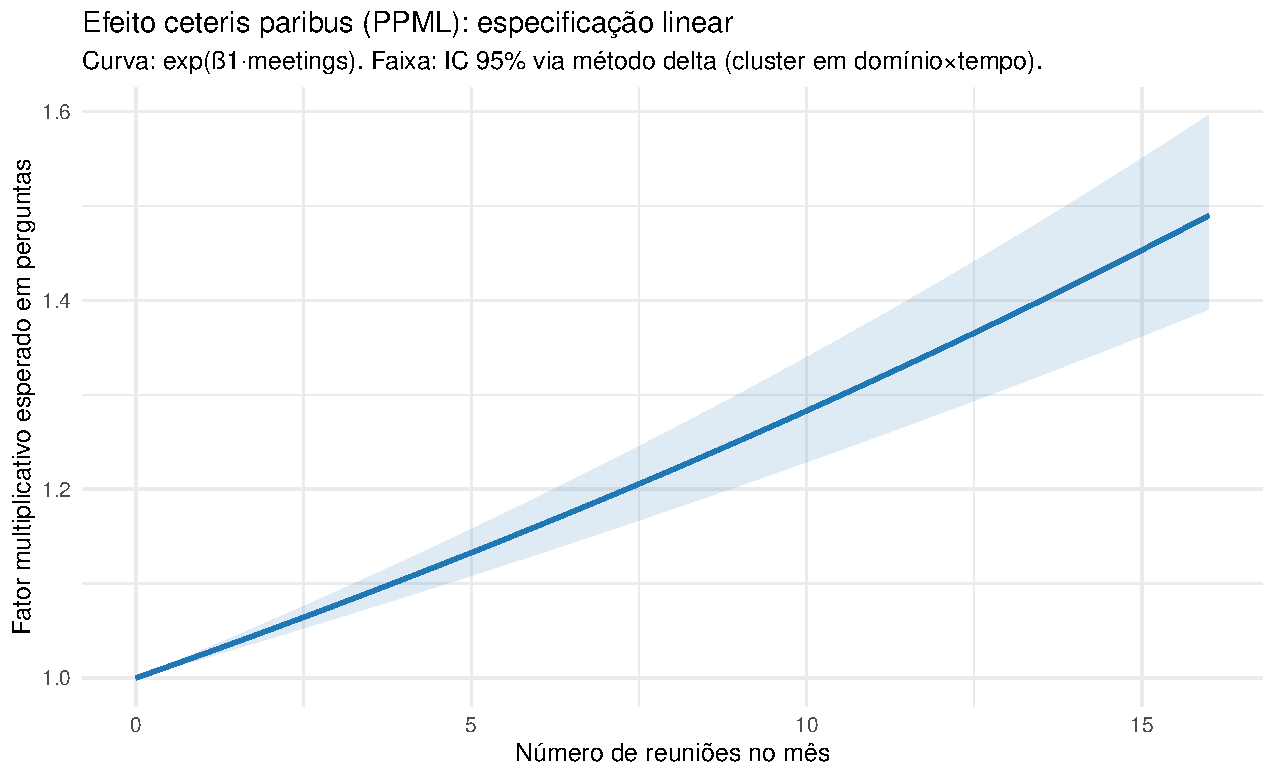
\includegraphics[width=\textwidth]{figures/h1_test/fig_effect_linear_ppml.pdf}
\caption{Efeito esperado ceteris paribus: especificação linear (\acrshort{ppml})}
\label{fig:effect_linear_ppml}
\note{A curva apresenta o fator multiplicativo esperado em perguntas como função do número de reuniões no mês, mantendo constantes os efeitos fixos (\(\exp(\hat{\beta}_1\cdot \textit{meetings})\)). A faixa sombreada corresponde ao intervalo de 95\% obtido via método delta com erros-padrão agrupados em domínio×tempo.}
\end{figure}

\begin{figure}[htbp]
\centering
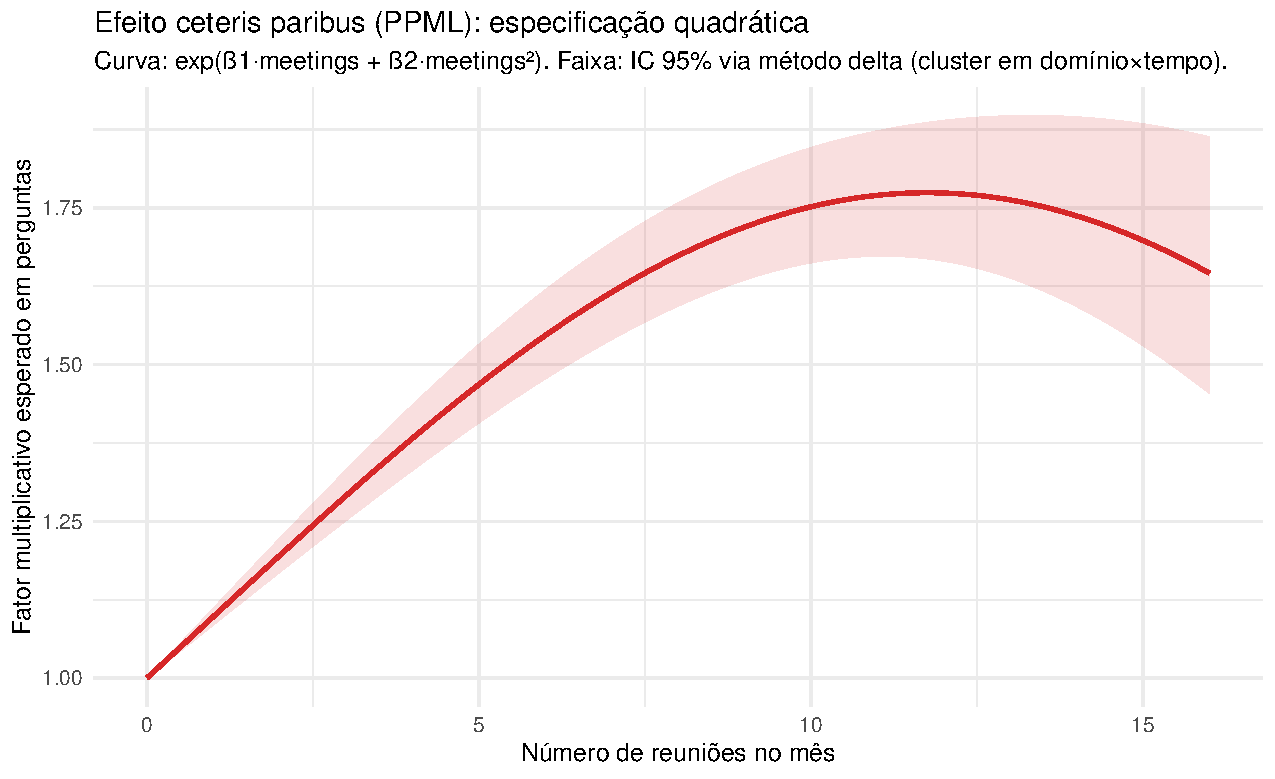
\includegraphics[width=\textwidth]{figures/h1_test/fig_effect_quadratic_ppml.pdf}
\caption{Efeito esperado ceteris paribus: especificação quadrática (\acrshort{ppml})}
\label{fig:effect_quadratic_ppml}
\note{A curva apresenta o fator multiplicativo esperado em perguntas como função do número de reuniões, permitindo retornos marginais decrescentes (\(\exp(\hat{\beta}_1\cdot \textit{meetings} + \hat{\beta}_2\cdot \textit{meetings}^2)\)). A faixa sombreada representa o IC de 95\% via método delta com a matriz de variância-covariância agrupada.}
\end{figure}

\autoref{tab:ppml_h1_both} mostra que o coeficiente de \textit{meetings} no modelo \acrshort{ppml} linear é positivo e estatisticamente significativo, evidenciando que aumentos na intensidade de lobbying associam-se a maior número de perguntas, \textit{ceteris paribus}. Na especificação quadrática, o termo linear permanece positivo enquanto o termo quadrático é negativo, indicando retornos marginais decrescentes: o impacto adicional de reuniões sobre perguntas diminui à medida que o volume de reuniões cresce.

Essa interpretação decorre da forma funcional do \acrshort{ppml} (\(\mathbb{E}[y\mid X]=\exp(X\beta)\)). No modelo linear, um acréscimo de uma unidade em \textit{meetings} altera a média condicional de perguntas em \(100\times(\mathrm{e}^{\hat{\beta}_1}-1)\%\). No modelo quadrático, o efeito marginal em log-média é \(\partial\log\mathbb{E}[y\mid X]/\partial\,\textit{meetings}=\hat{\beta}_1+2\hat{\beta}_2\,\textit{meetings}\). Com \(\hat{\beta}_2<0\), esse efeito declina com o nível de \textit{meetings}, isto é, há retornos marginais decrescentes. 

Em particular, a magnitude do termo quadrático é muito inferior ao efeito linear (0,098 vs. 0,004), o que indica retornos marginais decrescentes pequenos na faixa observada. Isso implica que atores com maior disponibilidade de recursos enfrentam pouca perda de eficácia ao intensificar o número de reuniões e, portanto, podem sustentar níveis muito mais altos de lobbying; tal padrão é consistente com a hipótese de que grandes players conseguem alavancar sua capacidade financeira para obter influência relativamente maior, mesmo diante de retornos marginais decrescentes.

% importante mencionar que esse efeito esperado é considerando o número de reuniões com apenas um parlamentar dentro de um único mês. Não considera o efeito total das reuniões que podem ser realizadas em meses diferentes. Não captura a dinâmica de uma organização realizar diversas reuniões com diversos parlamentares em meses diferents. Essa análise foi realizada para testar as hipóteses 2 e 3.

As curvas em \autoref{fig:effect_linear_ppml} e \autoref{fig:effect_quadratic_ppml} tornam essa dinâmica visual. A primeira apresenta um efeito multiplicativo crescente de forma monotônica (\(\exp(\hat{\beta}_1\,\allowbreak\textit{meetings})\)), com faixas de incerteza (IC 95\%) obtidas por método delta usando a matriz de variância-covariância com \textit{clustering} em domínio$\times$tempo e membro. A segunda permite curvatura (\(\exp(\hat{\beta}_1\,\allowbreak\textit{meetings}+\hat{\beta}_2\,\allowbreak\textit{meetings}^2)\)) e revela concavidade compatível com saturação de agenda: para níveis altos de \textit{meetings}, o ganho marginal em perguntas é menor. Em ambas as figuras, o eixo horizontal é mantido dentro do suporte observado dos dados para evitar extrapolações.

Do ponto de vista de identificação, os efeitos fixos por membro, país$\times$tempo e partido$\times$tempo controlam heterogeneidade não observada invariável e choques comuns, permitindo comparação \textit{within} do mesmo \acrshort{mpe} ao longo do tempo. A inferência usa erros-padrão agrupados em duas dimensões (domínio$\times$tempo; membro), acomodando dependência serial e seções cruzadas.

Em síntese, os resultados corroboram a Hipótese 1: há associação positiva entre lobbying e atividade de fiscalização medida por perguntas parlamentares, com evidência de retornos marginais decrescentes em níveis mais altos de \textit{meetings}. Essa conclusão é robusta a especificações alternativas consideradas.

A análise desagregada por domínios de políticas públicas revela que o efeito positivo das reuniões sobre a atividade parlamentar é consistente em praticamente todas as áreas temáticas consideradas. Conforme ilustrado na \autoref{fig:effect_linear_ppml_domains}, a estimativa do coeficiente associado a \textit{meetings} permanece positiva em todos os domínios, ainda que a magnitude do efeito varie entre eles. Por exemplo, domínios como "Agricultura" e "Educação" apresentam efeitos mais pronunciados, sugerindo que nesses setores o lobbying pode ser particularmente eficaz em estimular a apresentação de perguntas parlamentares. Já em áreas como "Economia e Comércio" ou "Tecnologia", embora o efeito também seja positivo, sua magnitude é ligeiramente inferior, o que pode refletir diferenças na dinâmica de atuação dos grupos de interesse ou na agenda dos parlamentares nesses temas.

\begin{figure}[htbp]
\centering
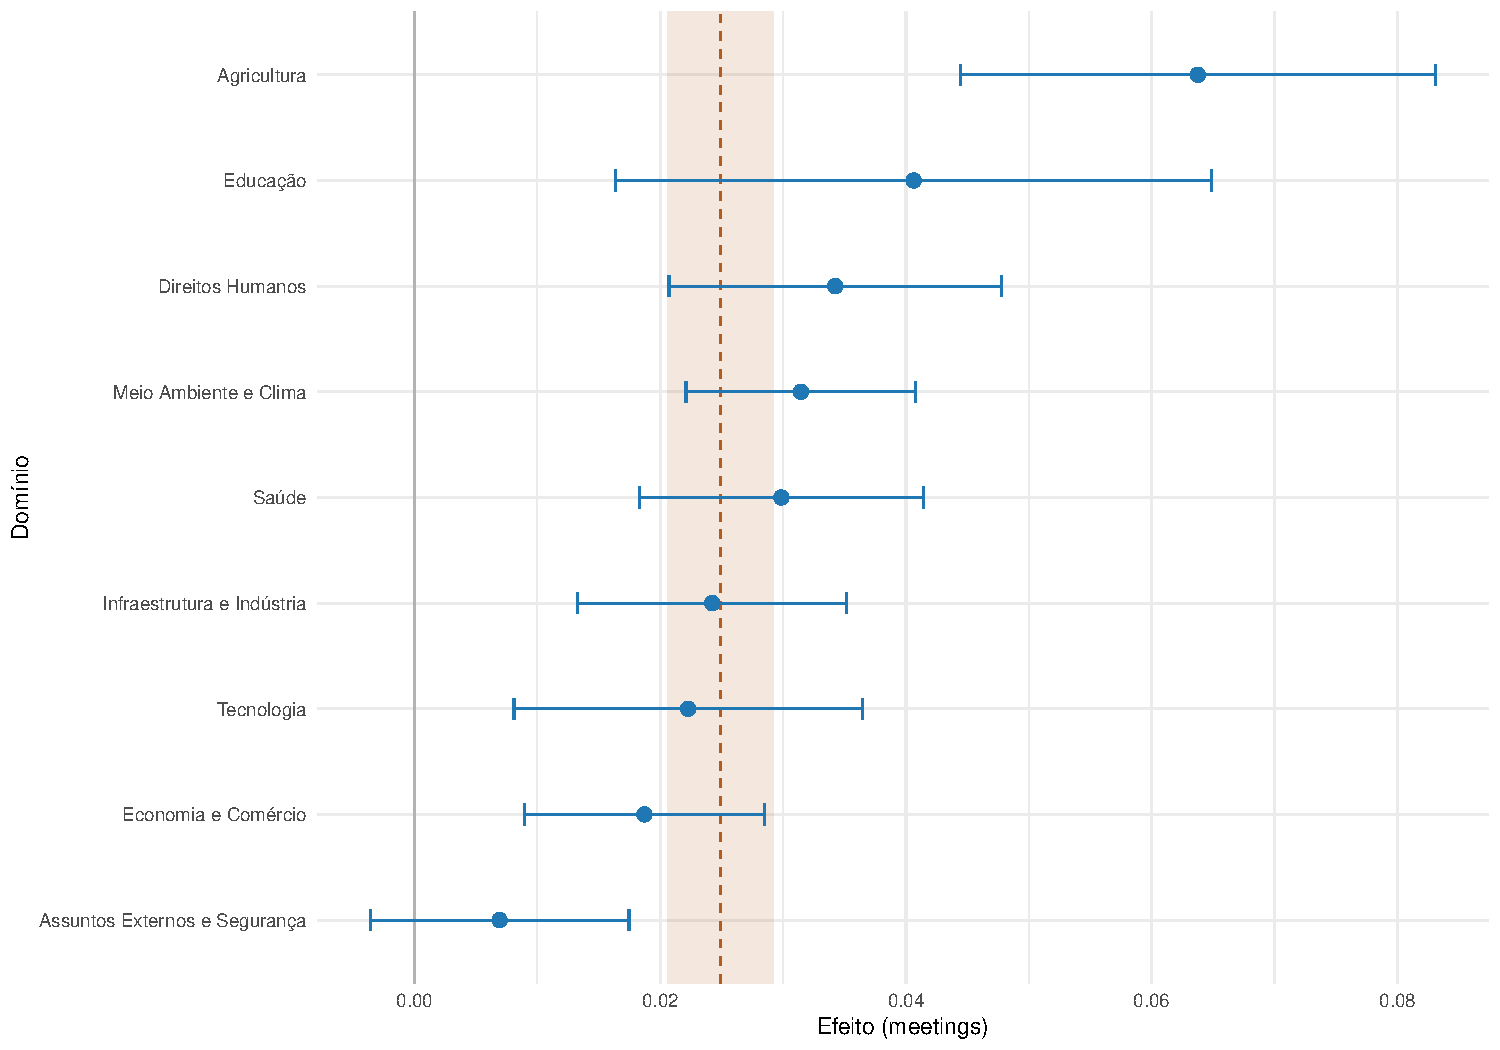
\includegraphics[width=\textwidth]{figures/fig_coeff_domains.pdf}
\caption{Efeito esperado \textit{ceteris paribus}: especificação linear (\acrshort{ppml}) para cada domínio}
\label{fig:effect_linear_ppml_domains}
\note{Cada ponto azul representa a estimativa do coeficiente associado a \textit{meetings} para um domínio específico de políticas públicas, refletindo o efeito marginal esperado de reuniões sobre o número de perguntas parlamentares naquele domínio, mantidos constantes os efeitos fixos. As linhas horizontais correspondem aos intervalos de confiança de 95\% para cada estimativa, indicando a incerteza estatística. A linha tracejada vermelha indica o efeito médio estimado para todos os domínios, servindo como referência para comparação entre áreas temáticas.}
\end{figure}

Além disso, os intervalos de confiança indicam que, apesar de variações na precisão das estimativas entre domínios, o sinal positivo do efeito é robusto e estatisticamente distinto de zero na maioria dos casos. Isso reforça a conclusão de que a associação entre intensidade de lobbying e atividade de fiscalização parlamentar não se restringe a um setor específico, mas se manifesta de forma generalizada no Parlamento Europeu, ainda que com intensidades distintas conforme o contexto temático.

De modo geral, esses resultados sugerem que o impacto do lobbying sobre a produção de perguntas parlamentares é um fenômeno transversal aos diferentes campos de políticas públicas, evidenciando a relevância desse mecanismo de influência em múltiplas agendas legislativas.


% \begin{figure}[htbp]
%     \centering
%     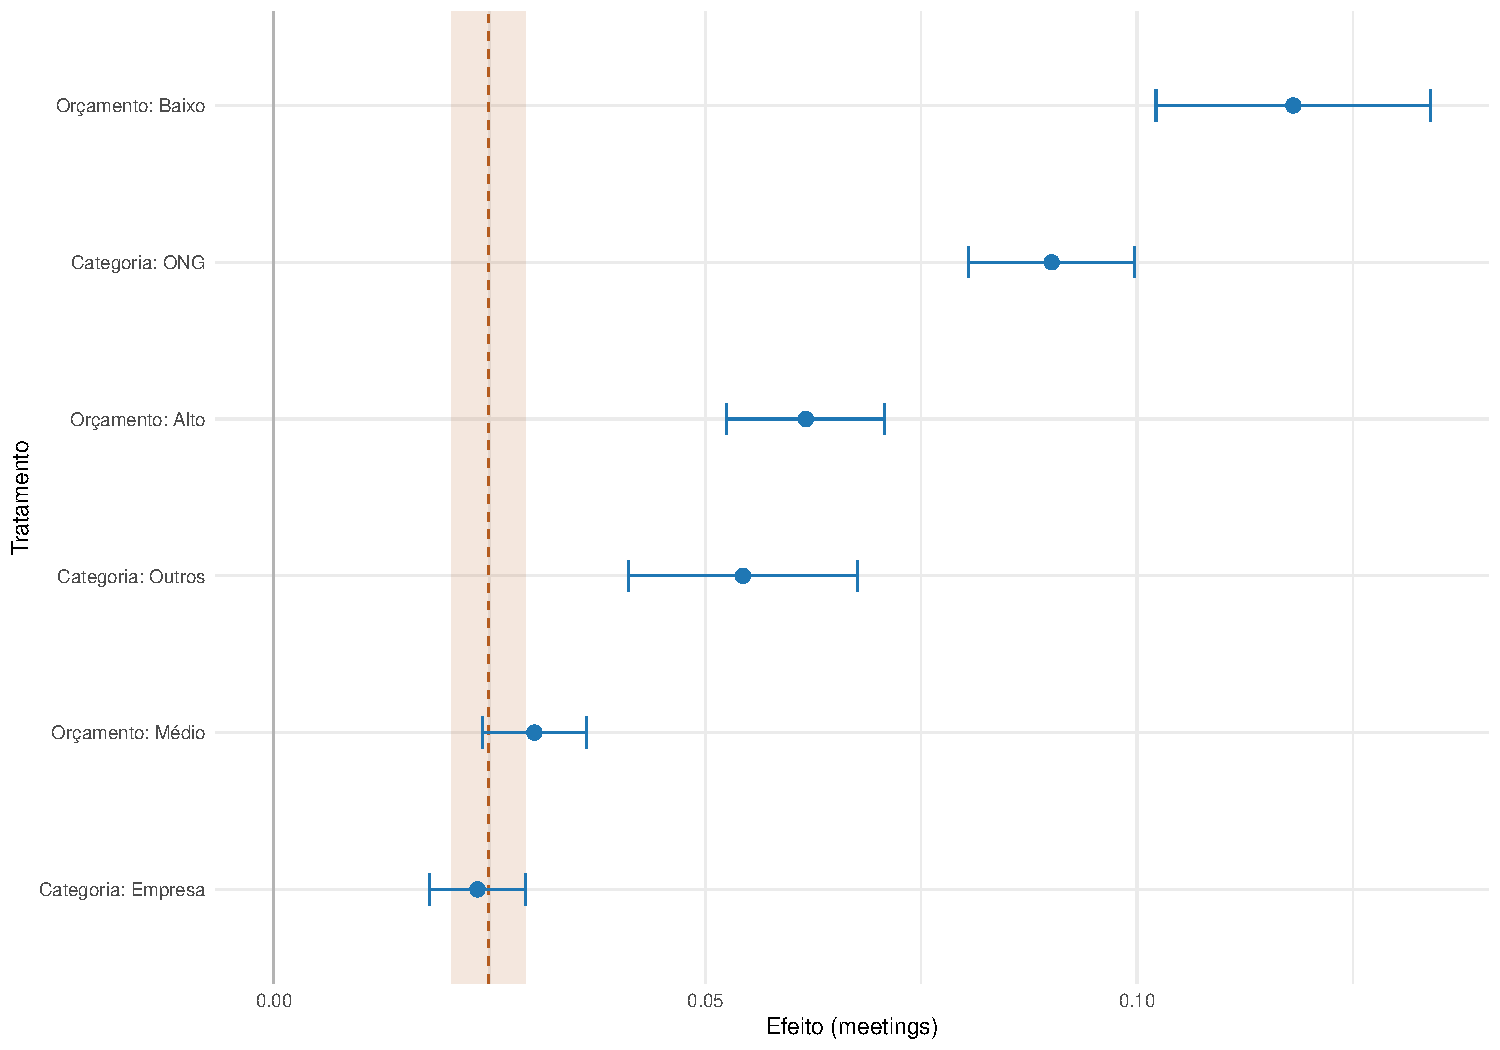
\includegraphics[width=\textwidth]{figures/fig_coeff_treatments_overall.pdf}
%     \caption{Efeito esperado \textit{ceteris paribus}: especificação linear (\acrshort{ppml}) para cada tratamento}
%     \label{fig:effect_linear_ppml_treatments}
%     \note{Cada ponto azul representa a estimativa do coeficiente associado a \textit{meetings} para um tratamento específico, refletindo o efeito marginal esperado de reuniões sobre o número de perguntas parlamentares, mantidos constantes os efeitos fixos. As linhas horizontais correspondem aos intervalos de confiança de 95\% para cada estimativa, indicando a incerteza estatística. A linha tracejada vermelha indica o efeito médio estimado para todos os tratamentos, servindo como referência para comparação entre tratamentos.}
% \end{figure}



\subsection{A Heterogeneidade do Efeito por Tipo de Ator}

A avaliação da Hipótese 2, que postula uma maior influência das empresas sobre a atividade parlamentar em comparação com outros atores, exige uma análise que transcenda a simples contagem de reuniões. Uma análise preliminar do efeito marginal por reunião, apresentada na Figura \ref{fig:effect_linear_ppml_treatments}, sugere que as \acrshort{ong}s, paradoxalmente, exercem uma influência maior por encontro. Este resultado, embora contraintuitivo, destaca a necessidade de um modelo mais completo que considere a heterogeneidade dos atores de lobby.

\begin{figure}[htbp]
    \centering
    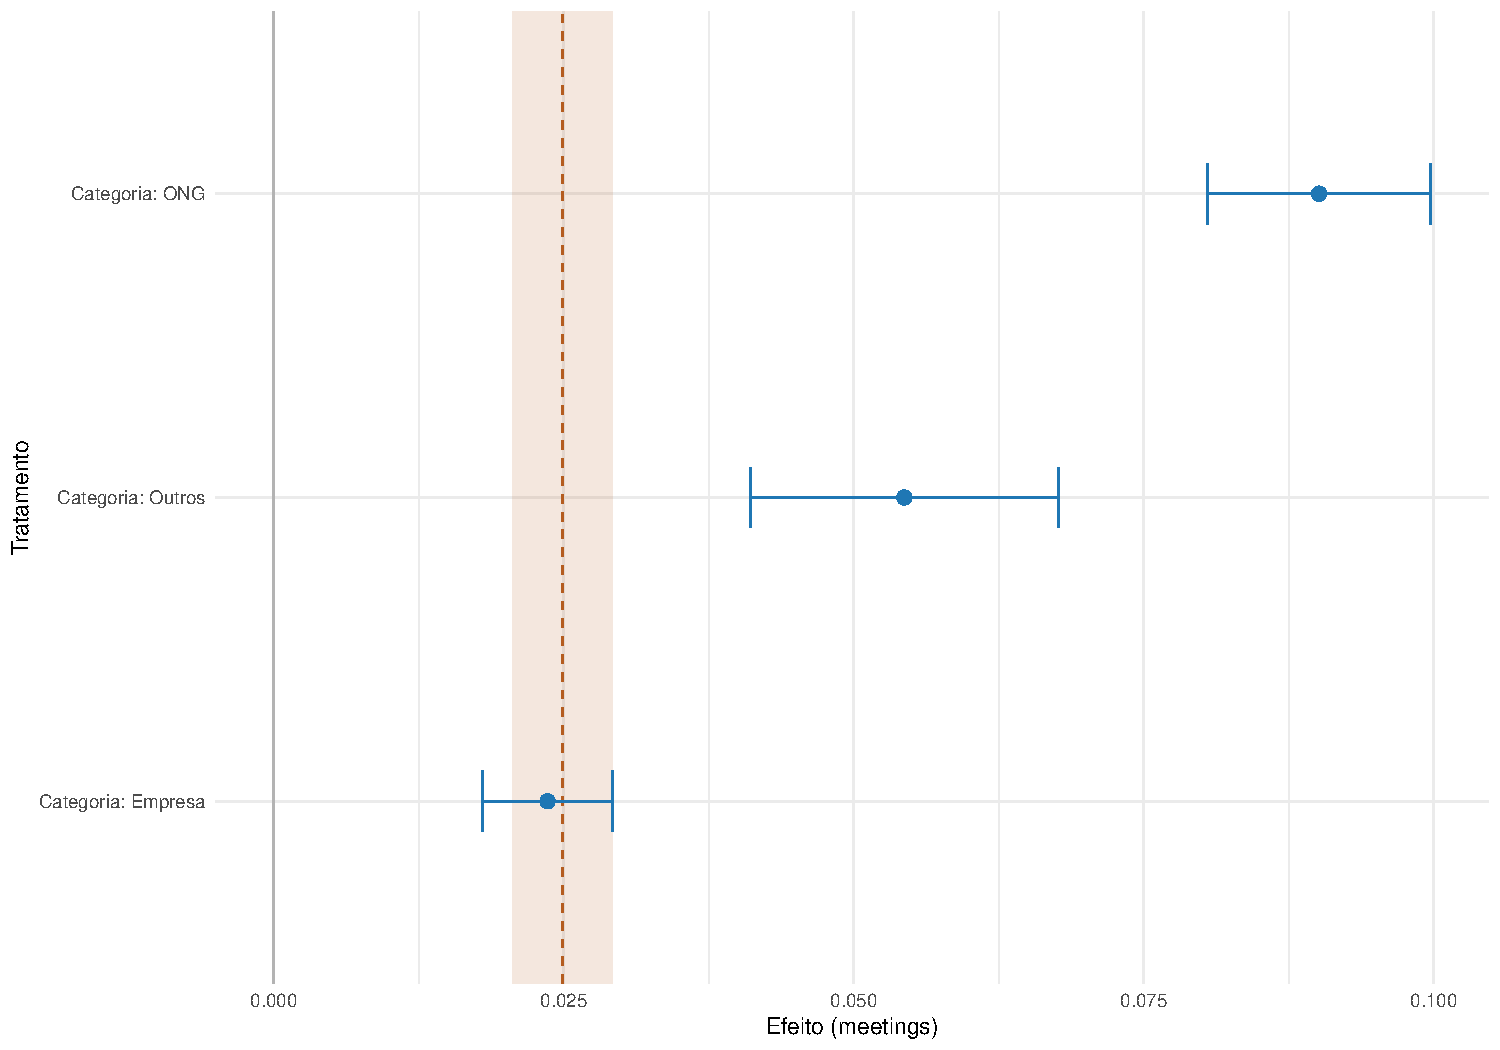
\includegraphics[width=\textwidth]{figures/h2_test/fig_coeff_treatments_overall.pdf}
    \caption{Efeito marginal por tipo de ator: especificação \acrshort{ppml}}
    \label{fig:effect_linear_ppml_treatments}
    \note{Cada ponto representa a estimativa do coeficiente para \textit{reuniões}, associado a um tipo de ator (tratamento), refletindo o efeito marginal esperado de uma única reunião sobre o número de perguntas parlamentares, mantendo os efeitos fixos constantes. As linhas horizontais indicam os intervalos de confiança de 95\%. A faixa vertical sombreada representa o intervalo de confiança do efeito médio geral, servindo como referência.}
\end{figure}

O efeito marginal isolado, contudo, é insuficiente para um teste robusto da hipótese. A influência total de um grupo de interesse não depende apenas da \textit{eficácia} de cada reunião, mas também da sua capacidade de assegurar \textit{acesso} -- isto é, o volume de reuniões que consegue realizar. Argumentamos que o impacto total é uma função dessas duas componentes: a frequência do acesso e a eficácia da persuasão em cada encontro.

Para capturar essa dualidade, adotamos uma estratégia de modelagem em duas etapas que decompõe o processo de lobby da seguinte forma:
\begin{itemize}
    \item \textbf{Acesso (Frequência):} O processo pelo qual um lobista garante reuniões com os \acrshort{mpe}s. Esta etapa, modelada com uma regressão Binomial Negativa, responde à pergunta: \textit{"Quantas reuniões um determinado lobista consegue obter?"}
    \item \textbf{Persuasão (Eficácia):} O processo pelo qual um lobista utiliza uma reunião para influenciar a atividade de um \acrshort{mpe}. Esta etapa, modelada com \acrshort{ppml}, responde à pergunta: \textit{"Quão eficaz é uma única reunião para gerar atividade parlamentar?"}
\end{itemize}

Esta abordagem permite-nos decompor e compreender os mecanismos através dos quais diferentes atores exercem influência.

Para estimar o volume de reuniões (Acesso) - Etapa 1 -, utilizamos um modelo de regressão Binomial Negativo, apropriado para dados de contagem com sobredispersão. A variável dependente é o número de reuniões que um lobista realiza, e as variáveis explicativas incluem o orçamento de lobby, a categoria do ator (\acrshort{ong}, Empresa, Outros) e um termo de interação entre orçamento e categoria, além de controles setoriais e geográficos.

O coeficiente de interação entre ser uma empresa e o orçamento de lobby é particularmente revelador. Um resultado positivo e estatisticamente significativo para este termo indica que as empresas não só tendem a realizar mais reuniões em média, mas também demonstram uma "eficiência alocativa" superior: cada aumento percentual no seu orçamento se traduz num aumento maior no número de reuniões em comparação com as \acrshort{ong}s. A Figura \ref{fig:h2_pred_meetings} ilustra essa dinâmica, mostrando o número esperado de reuniões em função do orçamento.

\begin{figure}[htbp]
    \centering
    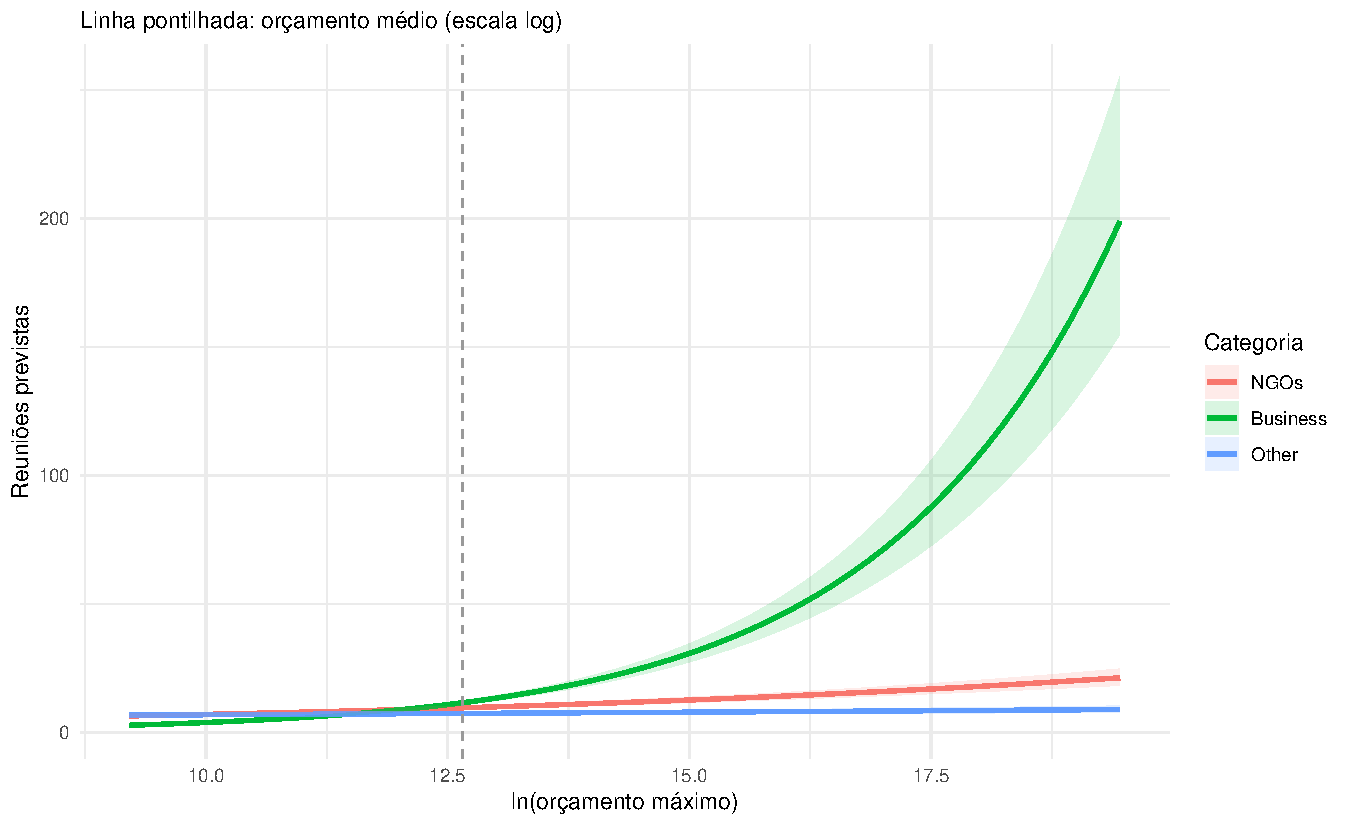
\includegraphics[width=\textwidth]{figures/h2_test/fig_pred_meetings_vs_budget_centered_by_category.pdf}
    \caption{Previsão do número de reuniões por categoria e orçamento}
    \label{fig:h2_pred_meetings}
    \note{O gráfico exibe o número esperado de reuniões (eixo Y) em função do logaritmo do orçamento de lobby (eixo X), com base no modelo Binomial Negativo. As curvas representam a previsão para cada categoria de ator, mantendo as demais variáveis em seus valores médios ou modais. A linha tracejada vertical indica o orçamento médio na amostra. As áreas sombreadas correspondem aos intervalos de confiança de 95\%.}
\end{figure}

Observa-se um ponto de inflexão: abaixo de um orçamento de aproximadamente \$27.000 ($\approx e^{10.2}$), as \acrshort{ong}s tendem a realizar mais reuniões. Acima desse limiar, a capacidade das empresas de converter recursos financeiros em acesso torna-se proeminente, e a disparidade cresce exponencialmente com o orçamento.

Para estimar o efeito agregado (Etapa 2), combinamos os resultados das duas etapas, multiplicando o número esperado de reuniões (o \textit{Acesso}, da Etapa 1) pelo efeito marginal por reunião (a \textit{Persuasão}, da Figura \ref{fig:effect_linear_ppml_treatments}) para cada categoria de ator e nível de orçamento. O resultado, ilustrado na Figura \ref{fig:h2_total_effects}, representa uma aproximação de primeira ordem do impacto total do lobby.

\begin{figure}[htbp]
    \centering
    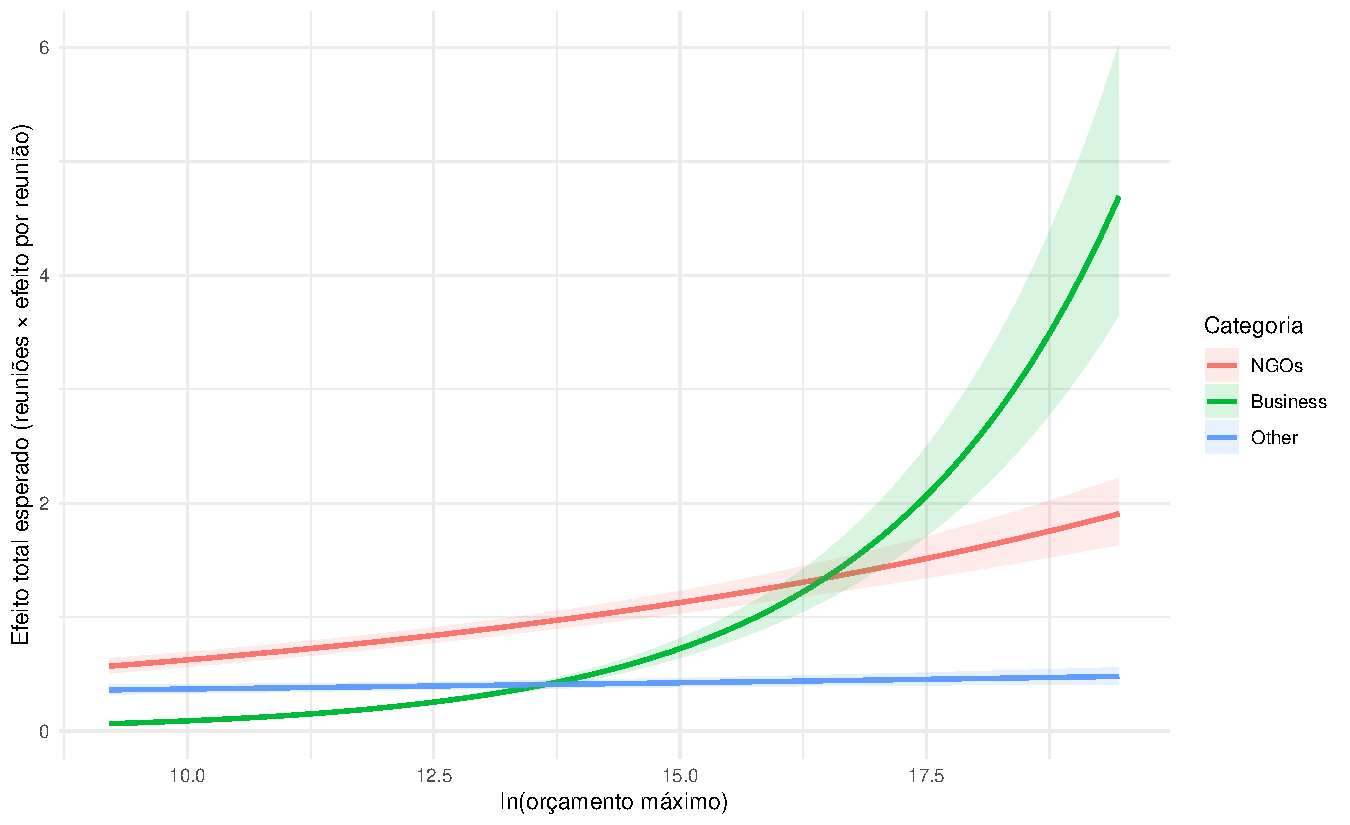
\includegraphics[width=\textwidth]{figures/h2_test/fig_total_effect_vs_budget_by_category.pdf}
    \caption{Efeito total estimado por categoria e orçamento}
    \label{fig:h2_total_effects}
    \note{O gráfico representa o efeito total esperado, calculado como o produto do número previsto de reuniões (da Figura \ref{fig:h2_pred_meetings}) e do coeficiente de efeito marginal por reunião (da Figura \ref{fig:effect_linear_ppml_treatments}). O eixo Y representa o aumento esperado no número de perguntas parlamentares.}
\end{figure}

A análise do efeito total revela uma relação complexa e não-linear. Embora uma única reunião com uma \acrshort{ong} seja, em média, mais influente, a superioridade das empresas em garantir um grande volume de acesso, especialmente quando dispõem de orçamentos elevados, reverte essa vantagem. Para orçamentos abaixo de \$8,8 milhões ($\approx e^{16}$), o efeito total das \acrshort{ong}s permanece superior. No entanto, acima de \$40 milhões ($\approx e^{17.5}$), o efeito agregado das empresas torna-se substancialmente maior.

Estes resultados oferecem um suporte nuançado à Hipótese 2 e dialogam diretamente com a literatura sobre os mecanismos de influência do lobby. A influência das empresas não é incondicionalmente superior, mas torna-se dominante quando alavancada por vastos recursos financeiros, um achado que se alinha com a discussão sobre a desigualdade de representação \cite{mahoney_lobbying_2007}. A decomposição do efeito em "acesso" e "persuasão" permite-nos explorar as diferentes naturezas dos recursos mobilizados pelos atores, conforme aponta a literatura \cite{de_figueiredo_advancing_2014, Pop2013Lobbying}.

A maior eficácia marginal por reunião das \acrshort{ong}s pode ser interpretada à luz do seu capital reputacional e da sua legitimidade percebida \cite{bunea2018legitimacy}. Do ponto de vista do comportamento parlamentar, interagir com \acrshort{ong}s pode ser uma estratégia de \textit{vote-seeking} para os \acrshort{mpe}s, que buscam sinalizar alinhamento com causas de interesse público e, assim, aumentar seu apelo eleitoral \cite{Ibenskas2021, mayhew2004congress}.

Por outro lado, a capacidade das grandes corporações de converter recursos financeiros em um volume massivo de acesso aponta para outro mecanismo de influência: a subsidiação de informação. Para atingir seus objetivos de carreira (\textit{career-seeking}) e de formulação de políticas (\textit{policy-seeking}), os parlamentares necessitam de informação técnica e especializada \cite{daniel2015career, kluver_informational_2012}. As grandes empresas, com seus recursos, estão em posição privilegiada para fornecer este subsídio informacional, estabelecendo uma relação de troca \cite{huwyler_no_2023} que lhes garante um acesso privilegiado e contínuo. Assim, a capacidade de "saturar" o ambiente informacional com interações frequentes parece ser um fator decisivo para a sua influência agregada.

É importante notar que esta abordagem metodológica assenta na premissa de \textit{separabilidade} entre os processos de "acesso" e "persuasão". Esta premissa implica que, após controlarmos pelas variáveis observáveis (como o orçamento), os fatores não observados que tornam um lobista eficaz em garantir reuniões são estatisticamente independentes dos fatores não observados que o tornam influente durante essas reuniões. A suposição de separabilidade poderia ser violada se, por exemplo, uma "qualidade" ou "reputação" intrínseca do lobista, não capturada pelo modelo, afetasse simultaneamente a sua capacidade de agendar reuniões e a recetividade dos parlamentares às suas propostas. Nesse cenário, a multiplicação dos efeitos poderia levar a uma estimativa enviesada do impacto total.

Em suma, os resultados indicam que, embora o discurso das \acrshort{ong}s possa ter maior ressonância por interação, a capacidade financeira das grandes empresas permite-lhes superar essa desvantagem através de uma presença quantitativamente esmagadora, confirmando a importância crítica dos recursos na determinação da influência política.
\subsubsection{Teste da hipótese 3: O Efeito do Lobby em Temas Salientes}

A Hipótese 3 postula que, em temas de maior saliência, o lobby exercido por organizações não empresariais (como as \acrshort{ong}s) tem uma maior probabilidade de influenciar a atividade legislativa dos \acrshort{mpe}s em comparação com o lobby de organizações empresariais. A lógica subjacente é que, quando um tema está sob intenso escrutínio público, os parlamentares se tornam mais sensíveis a argumentos que ressoam com a opinião pública e a interesses difusos, frequentemente representados por \acrshort{ong}s.

Para testar esta hipótese, mantivemos a estrutura do modelo \acrshort{ppml} com efeitos fixos, garantindo a consistência com as análises anteriores. A principal diferença metodológica foi a introdução de uma variável para capturar a saliência de um tema e a sua interação com os diferentes tipos de lobistas.

A saliência foi operacionalizada como uma proxy baseada na intensidade da atividade de lobby, uma abordagem que encontra respaldo na literatura \cite{baumgartner2010agendas}. Especificamente, criamos uma variável (salience\_std) que mede o volume total de reuniões de lobby dentro de cada domínio temático para cada período mensal, padronizada para ter média zero e desvio padrão um. Um valor mais alto nesta variável indica que um tema atraiu mais atenção de todos os grupos de interesse, sendo, portanto, considerado mais saliente.

O modelo econométrico foi então especificado para incluir termos de interação entre cada categoria de lobista (Empresa, \acrshort{ong}, Outros) e a variável de saliência, apresentado na Equação \ref{eq:modelo_h3}. Esta especificação permite-nos estimar como o efeito marginal de uma reunião de cada tipo de ator varia em função do nível de saliência do tema. Os resultados da regressão estão sumarizados na Tabela \ref{tab:h3_interaction} e visualizados no gráfico de efeitos marginais na Figura \ref{fig:h3_marginal_effects}.

\begin{table}
\centering
\begin{talltblr}[         %% tabularray outer open
entry=none,label=none,
note{}={+ p \num{< 0.1}, * p \num{< 0.05}, ** p \num{< 0.01}, *** p \num{< 0.001}},
]                     %% tabularray outer close
{                     %% tabularray inner open
colspec={Q[]Q[]},
column{2}={}{halign=c,},
column{1}={}{halign=l,},
hline{10}={1-2}{solid, black, 0.05em},
}                     %% tabularray inner close
\toprule
& PPML com Interação (H3) \\ \midrule %% TinyTableHeader
Empresa (base) & \num{0.035}*** \\
& (\num{0.006}) \\
ONG (base) & \num{0.090}*** \\
& (\num{0.006}) \\
Outros (base) & \num{0.032}** \\
& (\num{0.010}) \\
Empresa x Saliência & \num{-0.022}*** \\
& (\num{0.005}) \\
Num.Obs. & \num{600237} \\
R2 & \num{0.253} \\
RMSE & \num{0.56} \\
Std.Errors & by: cl\_dt \\
FE: fe\_ct & X \\
FE: fe\_pt & X \\
FE: fe\_dt & X \\
\bottomrule
\end{talltblr}
\end{table}



\begin{figure}[htbp]
    \centering
    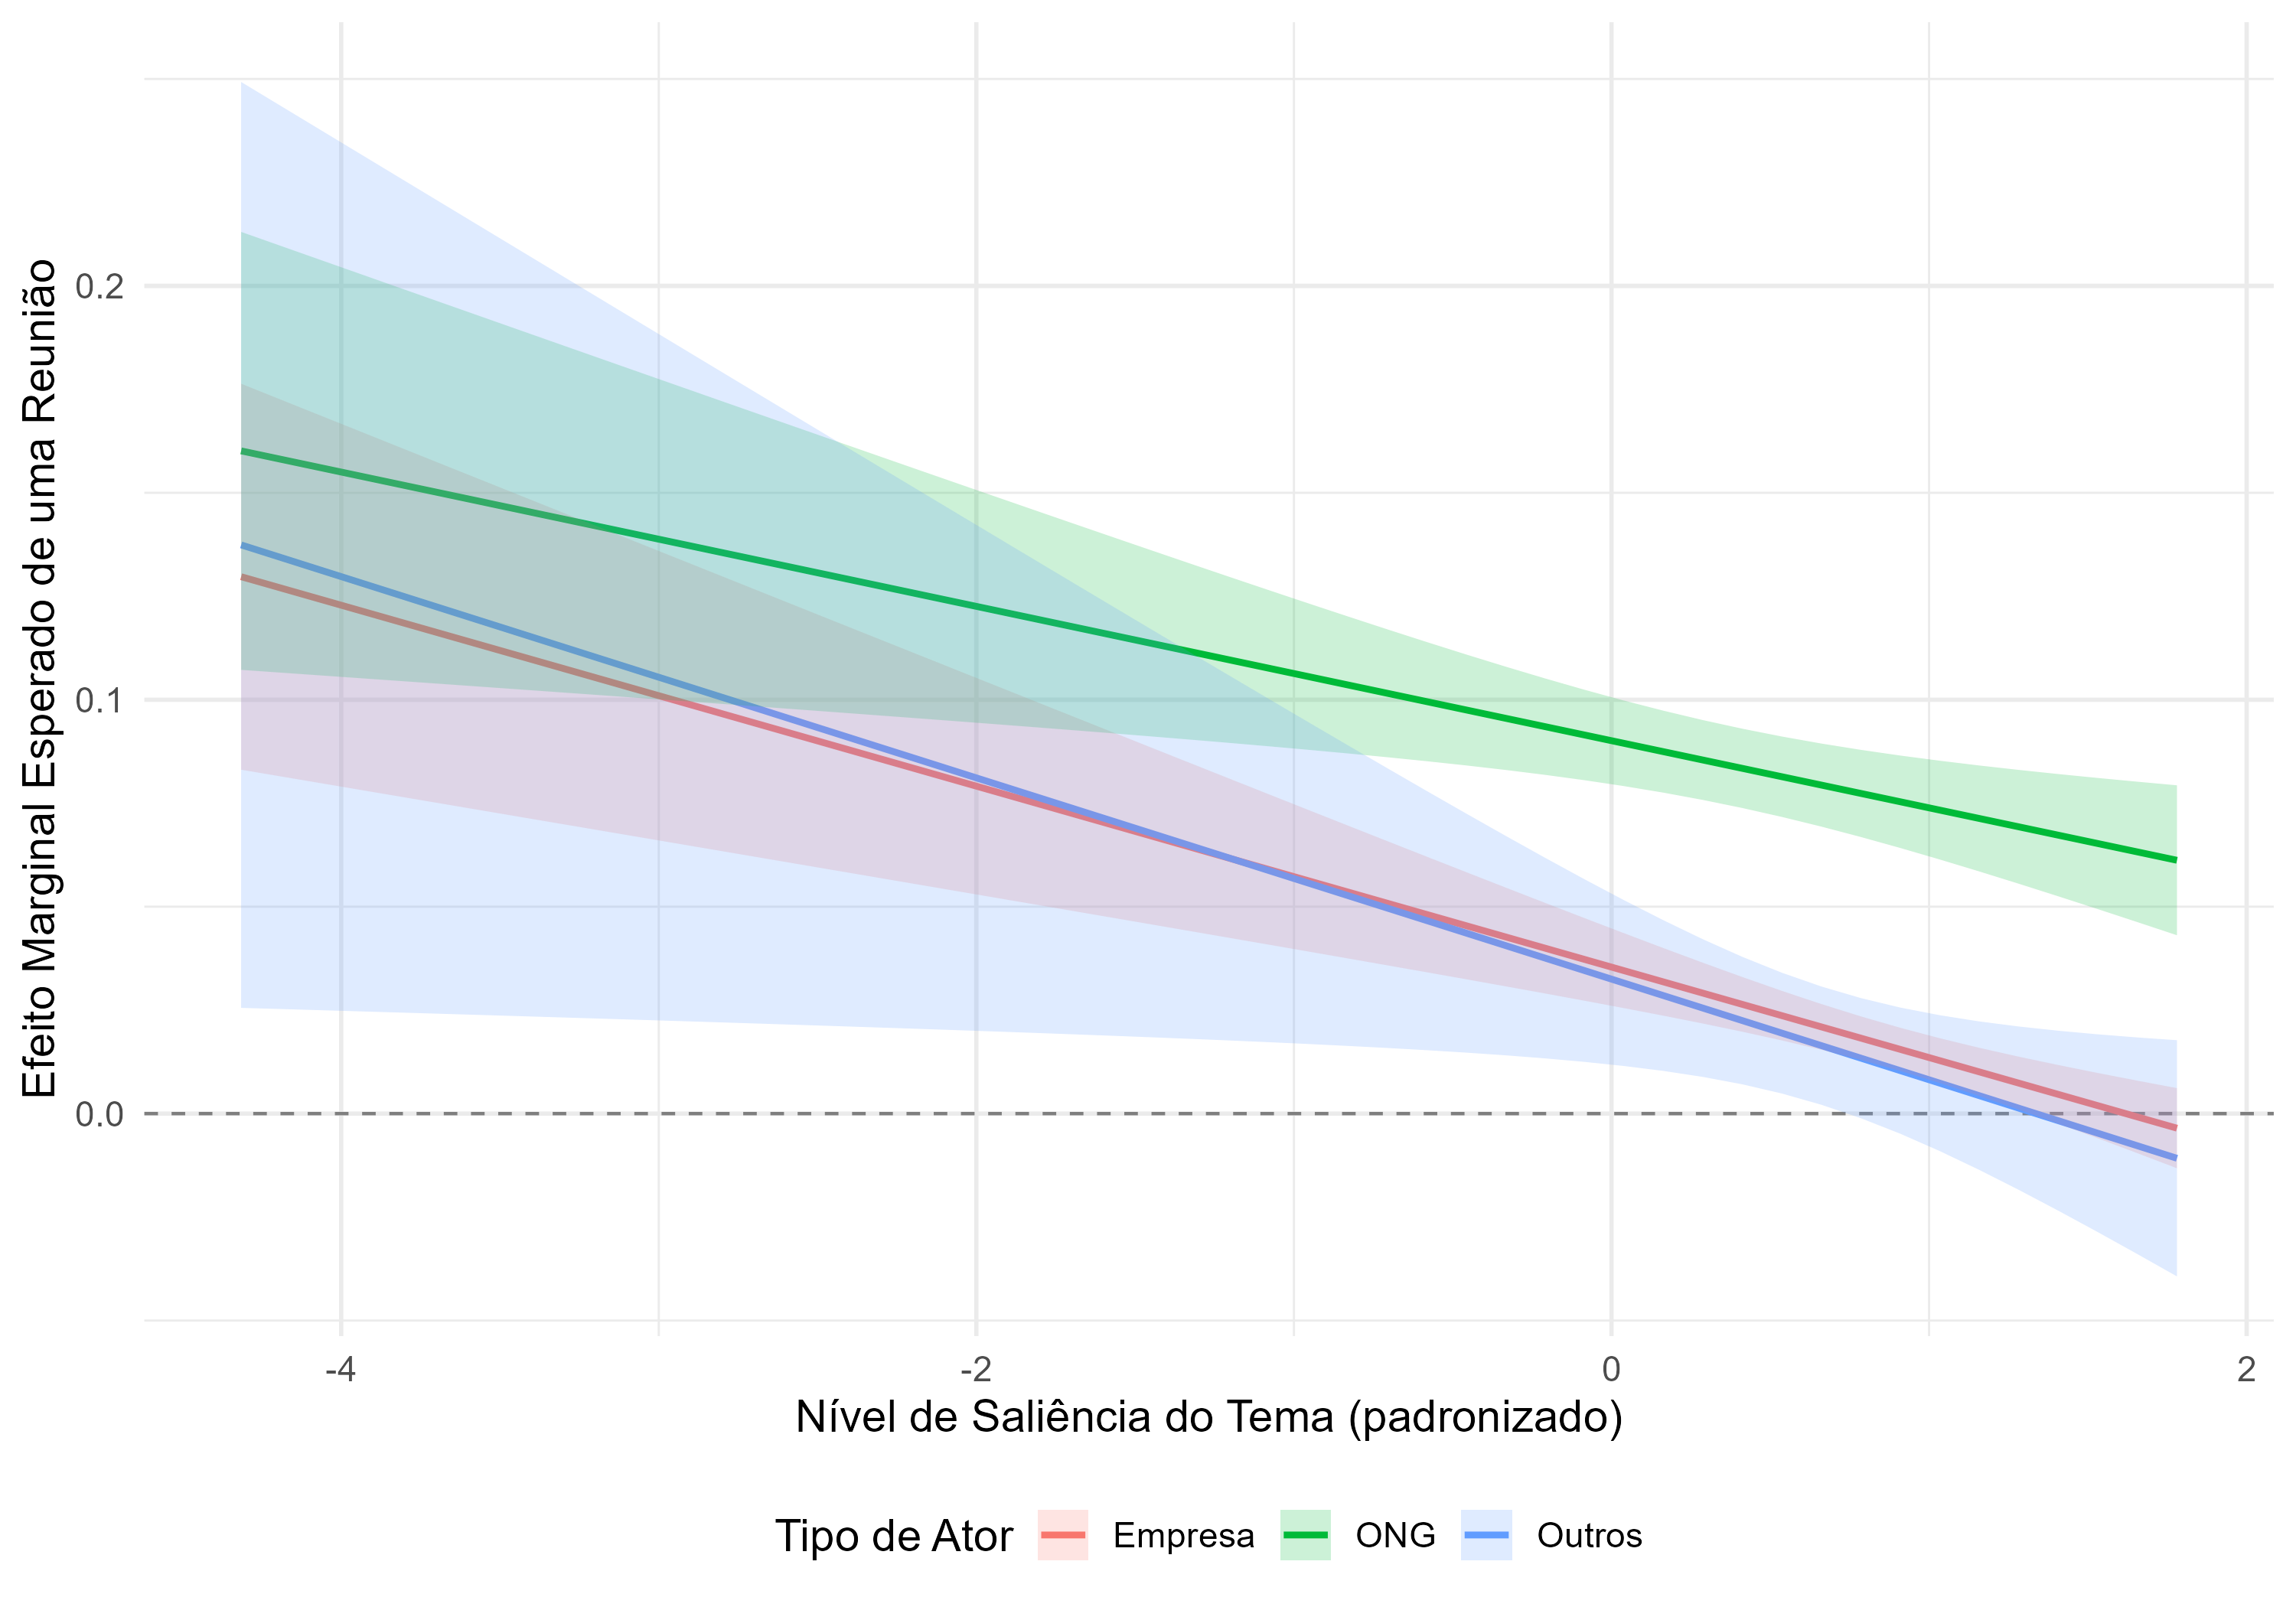
\includegraphics[width=\textwidth]{figures/h3_test/fig_h3_marginal_effects_manual.png}
    \caption{Efeito do Lobby Condicional à Saliência do Tema}
    \label{fig:h3_marginal_effects}
    \note{O gráfico exibe o efeito marginal esperado de uma única reunião sobre o número de perguntas parlamentares (eixo Y) em diferentes níveis de saliência do tema (eixo X). As linhas representam a estimativa para cada categoria de ator, e as áreas sombreadas correspondem aos intervalos de confiança de 95\%, calculados via bootstrap.}
\end{figure}

A análise revela um padrão complexo que contradiz parcialmente, mas também enriquece, a Hipótese 3. Contrariamente à expectativa de que o efeito das \acrshort{ong}s aumentaria com a saliência, observamos que o efeito marginal de uma reunião \textbf{diminui} para todos os grupos à medida que um tema se torna mais saliente (coeficiente negativo para todos os grupos nas variáveis de interação). Este achado está em forte alinhamento com a literatura, que sugere que a influência do lobby direto decresce quando a opinião pública e a atenção da mídia se intensificam, forçando os parlamentares a se alinharem a considerações eleitorais mais amplas \cite{mahoney_lobbying_2007, kollman1998outside}.

No entanto, a análise revela uma heterogeneidade crucial na taxa dessa diminuição. Três pontos principais se destacam na Figura \ref{fig:h3_marginal_effects}. Em temas de baixa saliência (à esquerda do gráfico), o efeito das \acrshort{ong}s é similar estatisticamente ao de empresas e outros atores. Isso pode ser observado pela intersecção das áreas sombreadas das linhas, que indicam o intervalo de confiança de 95\% das estimativas.
    
À medida que a saliência aumenta (movendo-se para a direita no gráfico), a vantagem comparativa das \acrshort{ong}s se acentua significativamente. O efeito do lobby de empresas e de outros atores decai rapidamente, enquanto o efeito das \acrshort{ong}s se mostra muito mais resiliente, diminuindo a uma taxa consideravelmente menor.
    
Em temas de alta saliência, onde a influência de empresas e outros grupos se torna estatisticamente indistinguível de zero (seus intervalos de confiança cruzam a linha pontilhada), o efeito das \acrshort{ong}s permanece positivo, robusto e estatisticamente significativo. É precisamente neste contexto de maior escrutínio público que a sua influência relativa se torna mais pronunciada.

Os resultados validam a Hipótese 3. Em temas de maior saliência, o lobby de organizações não empresariais é, de fato, mais eficaz em aumentar a atividade parlamentar em comparação com o lobby empresarial. A nuance importante é que essa maior eficácia não se manifesta como um aumento absoluto do efeito, mas sim como uma resiliência superior à pressão do escrutínio público, o que amplia a sua vantagem comparativa.

Esta descoberta dialoga diretamente com a teoria sobre os recursos do lobby e os incentivos parlamentares. Em temas de baixa saliência, os parlamentares, focados em seus objetivos de formulação de políticas (\textit{policy-seeking}), podem valorizar o subsídio informacional técnico fornecido por empresas. Contudo, quando um tema ganha visibilidade, os incentivos de reeleição (\textit{vote-seeking}) tornam-se dominantes \cite{mayhew2004congress}. Nesse contexto, alinhar-se a interesses empresariais pode ter um custo político elevado, enquanto responder a \acrshort{ong}s, que detêm maior capital de legitimidade \cite{bunea2018legitimacy}, reforça a imagem pública do parlamentar.

Os achados confirmam que a influência do lobby é altamente contextual e que, sob o escrutínio público, a vantagem se desloca para os atores percebidos como representantes de interesses mais amplos e difusos.

        \chapter{Resultados}
\label{chapter:resultados}
Este capítulo tem como objetivo apresentar e discutir os principais resultados empíricos da tese, respondendo às hipóteses formuladas e avaliando o impacto do lobby sobre a atividade legislativa no Parlamento Europeu. Inicialmente, são descritas as características dos lobistas e dos parlamentares presentes na amostra, bem como padrões descritivos das reuniões e perguntas parlamentares. Em seguida, são apresentados os resultados dos testes das hipóteses centrais, com análise dos efeitos estimados, heterogeneidades e mecanismos identificados. Por fim, o capítulo discute as implicações dos achados para o debate sobre influência política e transparência institucional.

\section{Lobby no Parlamento: atores, recursos e agendas}
\label{sec:resultados_descritica_lobistas}
A Tabela \ref{tab:dist_orgs_reunioes} apresenta a distribuição de lobistas e sua atividade (mensurada pelo número de reuniões) por categoria organizacional. Os dados revelam uma predominância de interesses empresariais, que constituem o maior grupo tanto em número de organizações (2.409) quanto em volume de reuniões (22.427). Em média, cada organização empresarial realizou 9,31 reuniões, a maior taxa entre as categorias. As ONGs figuram como o segundo grupo mais ativo, seguidas pela categoria "Outros".

\begin{table}[!htbp]
\centering
\caption{Distribuição de organizações, reuniões e reuniões por lobista, por categoria de organização}
\label{tab:dist_orgs_reunioes}
\begin{tabular}{lccc}
\hline
Categoria & Organizações & Reuniões & Reuniões por Organização \\
\hline
Empresarial & 2.409 & 22.427 & 9,31 \\
ONGs & 1.271 & 10.966 & 8,63 \\
Outros & 1.042 & 6.950 & 6,67 \\
\hline
Total & 4.722 & 40.343 & 8,54 \\
\hline  
\end{tabular}
\end{table}

Esses resultados corroboram uma vasta literatura que aponta para a assimetria de recursos e representação no universo do lobby. Interesses empresariais, que dispõem de maiores recursos financeiros, tendem a predominar na atividade de lobby \cite{de_figueiredo_advancing_2014}. No contexto específico da União Europeia, estudos demonstram que grupos empresariais e associações nacionais são os mais presentes \cite{dur20212wholobbies, eising2007institutional}, o que levou alguns autores a caracterizarem o sistema como um "pluralismo de elite" \cite{coen1997evolution, schmidt2006procedural}.

A intensidade da atividade, refletida no elevado número total de reuniões (40.343), sinaliza uma forte competição pelo acesso aos tomadores de decisão, um recurso considerado escasso pela literatura \cite{hall1990buying}. Embora os atores empresariais detenham mais acesso, a presença expressiva de ONGs indica um ambiente competitivo, e não monolítico. Essa coexistência sugere que diferentes tipos de organizações mobilizam recursos distintos para influenciar o processo político. Enquanto interesses empresariais podem alavancar recursos financeiros e expertise técnica, ONGs e outros grupos da sociedade civil podem recorrer a recursos como legitimidade, representatividade e apoio público para defender suas causas \cite{Coen2019, dur_measuring_2008}.

Portanto, a análise descritiva inicial já delineia uma das tensões centrais investigadas neste trabalho: o desequilíbrio de poder e recursos entre interesses empresariais e outros setores da sociedade, e como essa assimetria se manifesta na competição por influência política no \acrshort{pe}.


% Análise do orçamento máximo declarado
A análise do orçamento máximo declarado por categoria (Figura \ref{fig:budget_ln_boxplot}), em escala logarítmica, revela padrões distributivos distintos. O grupo empresarial, embora mais numeroso em quantidade de organizações, exibe a menor mediana de orçamento e uma distribuição notavelmente mais concentrada, o que sugere uma maior homogeneidade nos gastos com lobby declarados por essas entidades.

Em contrapartida, as ONGs e a categoria "Outros" apresentam medianas mais elevadas e uma variância substancialmente maior. Essa dispersão indica uma forte heterogeneidade interna, sugerindo a coexistência de organizações com recursos modestos e outras com orçamentos muito elevados, que influenciam a distribuição.

\begin{figure}[!htbp]
\centering
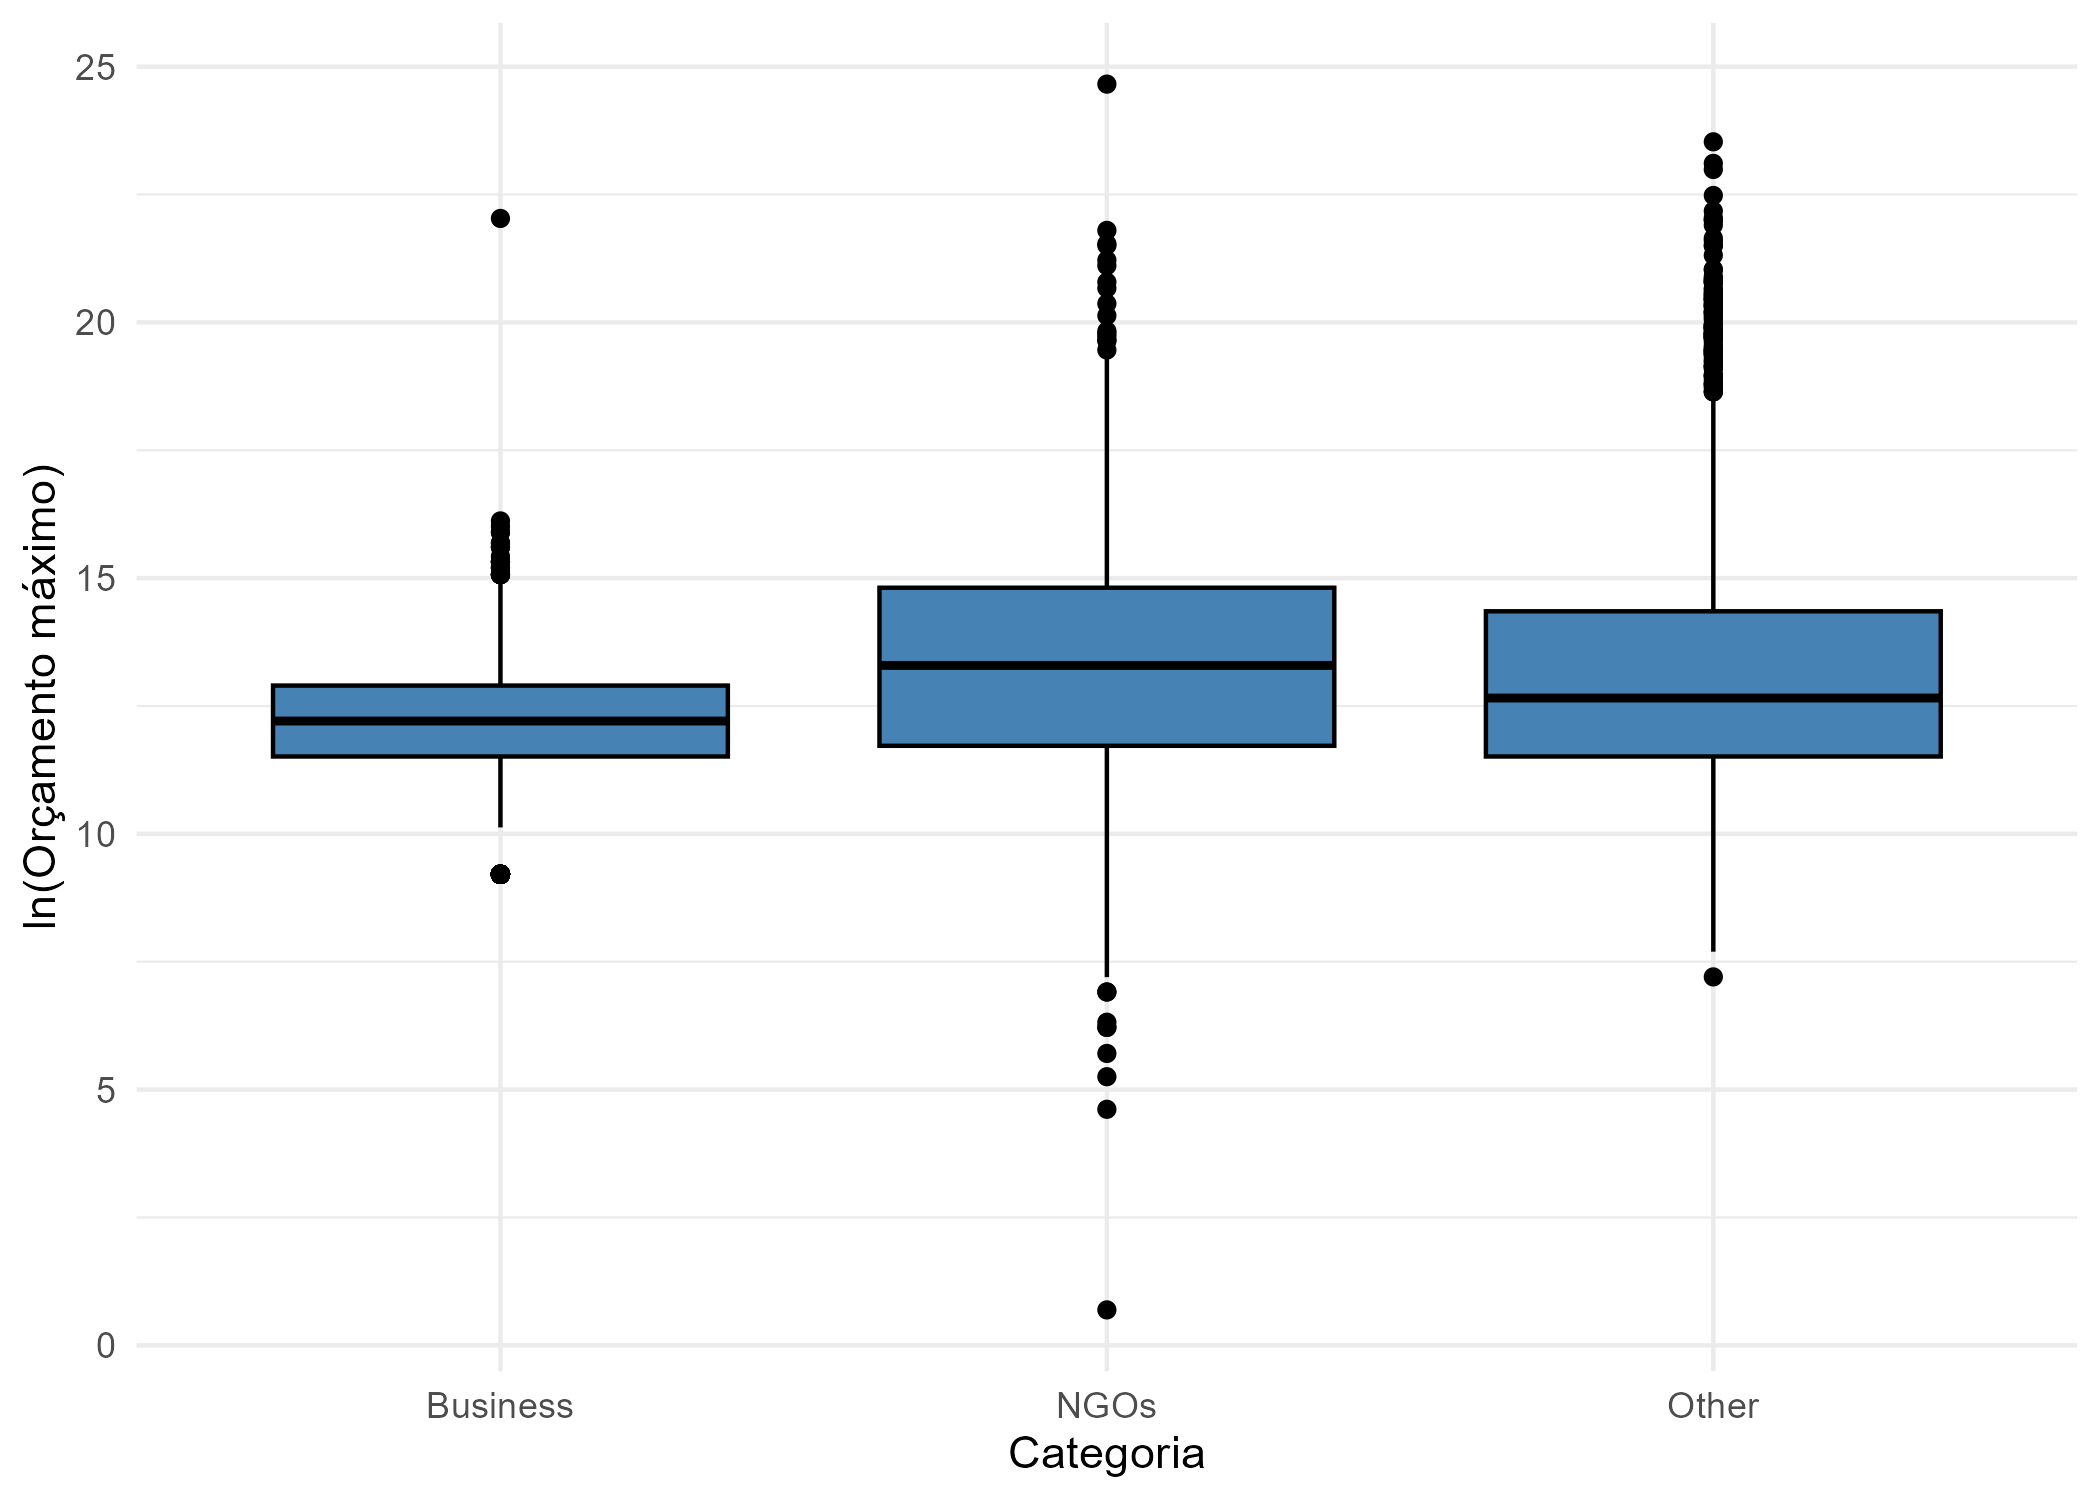
\includegraphics[width=0.75\textwidth]{figures/descriptives_lobbyists/boxplot_max_budget_by_category.png}
\caption{Distribuição de orçamento máximo declarado (\textit{ln(Orçamento Máximo Declarado)}) por categoria}
\label{fig:budget_ln_boxplot}
\end{figure}

Este achado é particularmente interessante, pois parece tensionar a premissa da literatura de que interesses empresariais dominam em termos de recursos financeiros \cite{de_figueiredo_advancing_2014, dur20212wholobbies}. Uma interpretação possível é que a categoria empresarial seja composta por um grande número de atores com gastos mais padronizados, enquanto as categorias de ONGs e "Outros" contêm algumas organizações muito grandes, cujos orçamentos massivos podem refletir campanhas de alto custo ou estruturas de financiamento distintas. A alta variância pode, ainda, ser um reflexo de diferentes estratégias: enquanto empresas podem ter um dispêndio mais constante, ONGs podem mobilizar grandes somas para temas de alta saliência, onde a opinião pública é um fator crucial \cite{mahoney_lobbying_2007}.

Adicionalmente, a concentração no grupo empresarial pode estar relacionada ao problema da ação coletiva \cite{olson1971logic}, onde muitas empresas optam por atuar por meio de associações — que podem estar classificadas na categoria "Outros". De todo modo, os dados reforçam que a relação entre recursos financeiros e influência não é direta \cite{simon_notes_1953}, e que a capacidade de mobilizar diferentes tipos de recursos — não apenas financeiros, mas também de legitimidade e informação \cite{Coen2019} — é central para a dinâmica do lobby na \acrshort{ue}.


% Distribuição geográfica
A análise da distribuição geográfica dos lobistas (Figura \ref{fig:country_distribution}) revela uma acentuada concentração em polos institucionais da União Europeia, com Bélgica (24,2\%), Alemanha (15,3\%) e França (10,1\%) abrigando a maioria das organizações. Este padrão corrobora a tese da vantagem da proximidade institucional: a presença massiva na Bélgica, sede da Comissão Europeia e de grande parte das atividades do Parlamento, e na França, que sedia as sessões plenárias do Parlamento em Estrasburgo, é uma resposta estratégica à complexa governança multinível da \acrshort{ue} \cite{richardson2000government}.

\begin{figure}[!htbp]
\centering
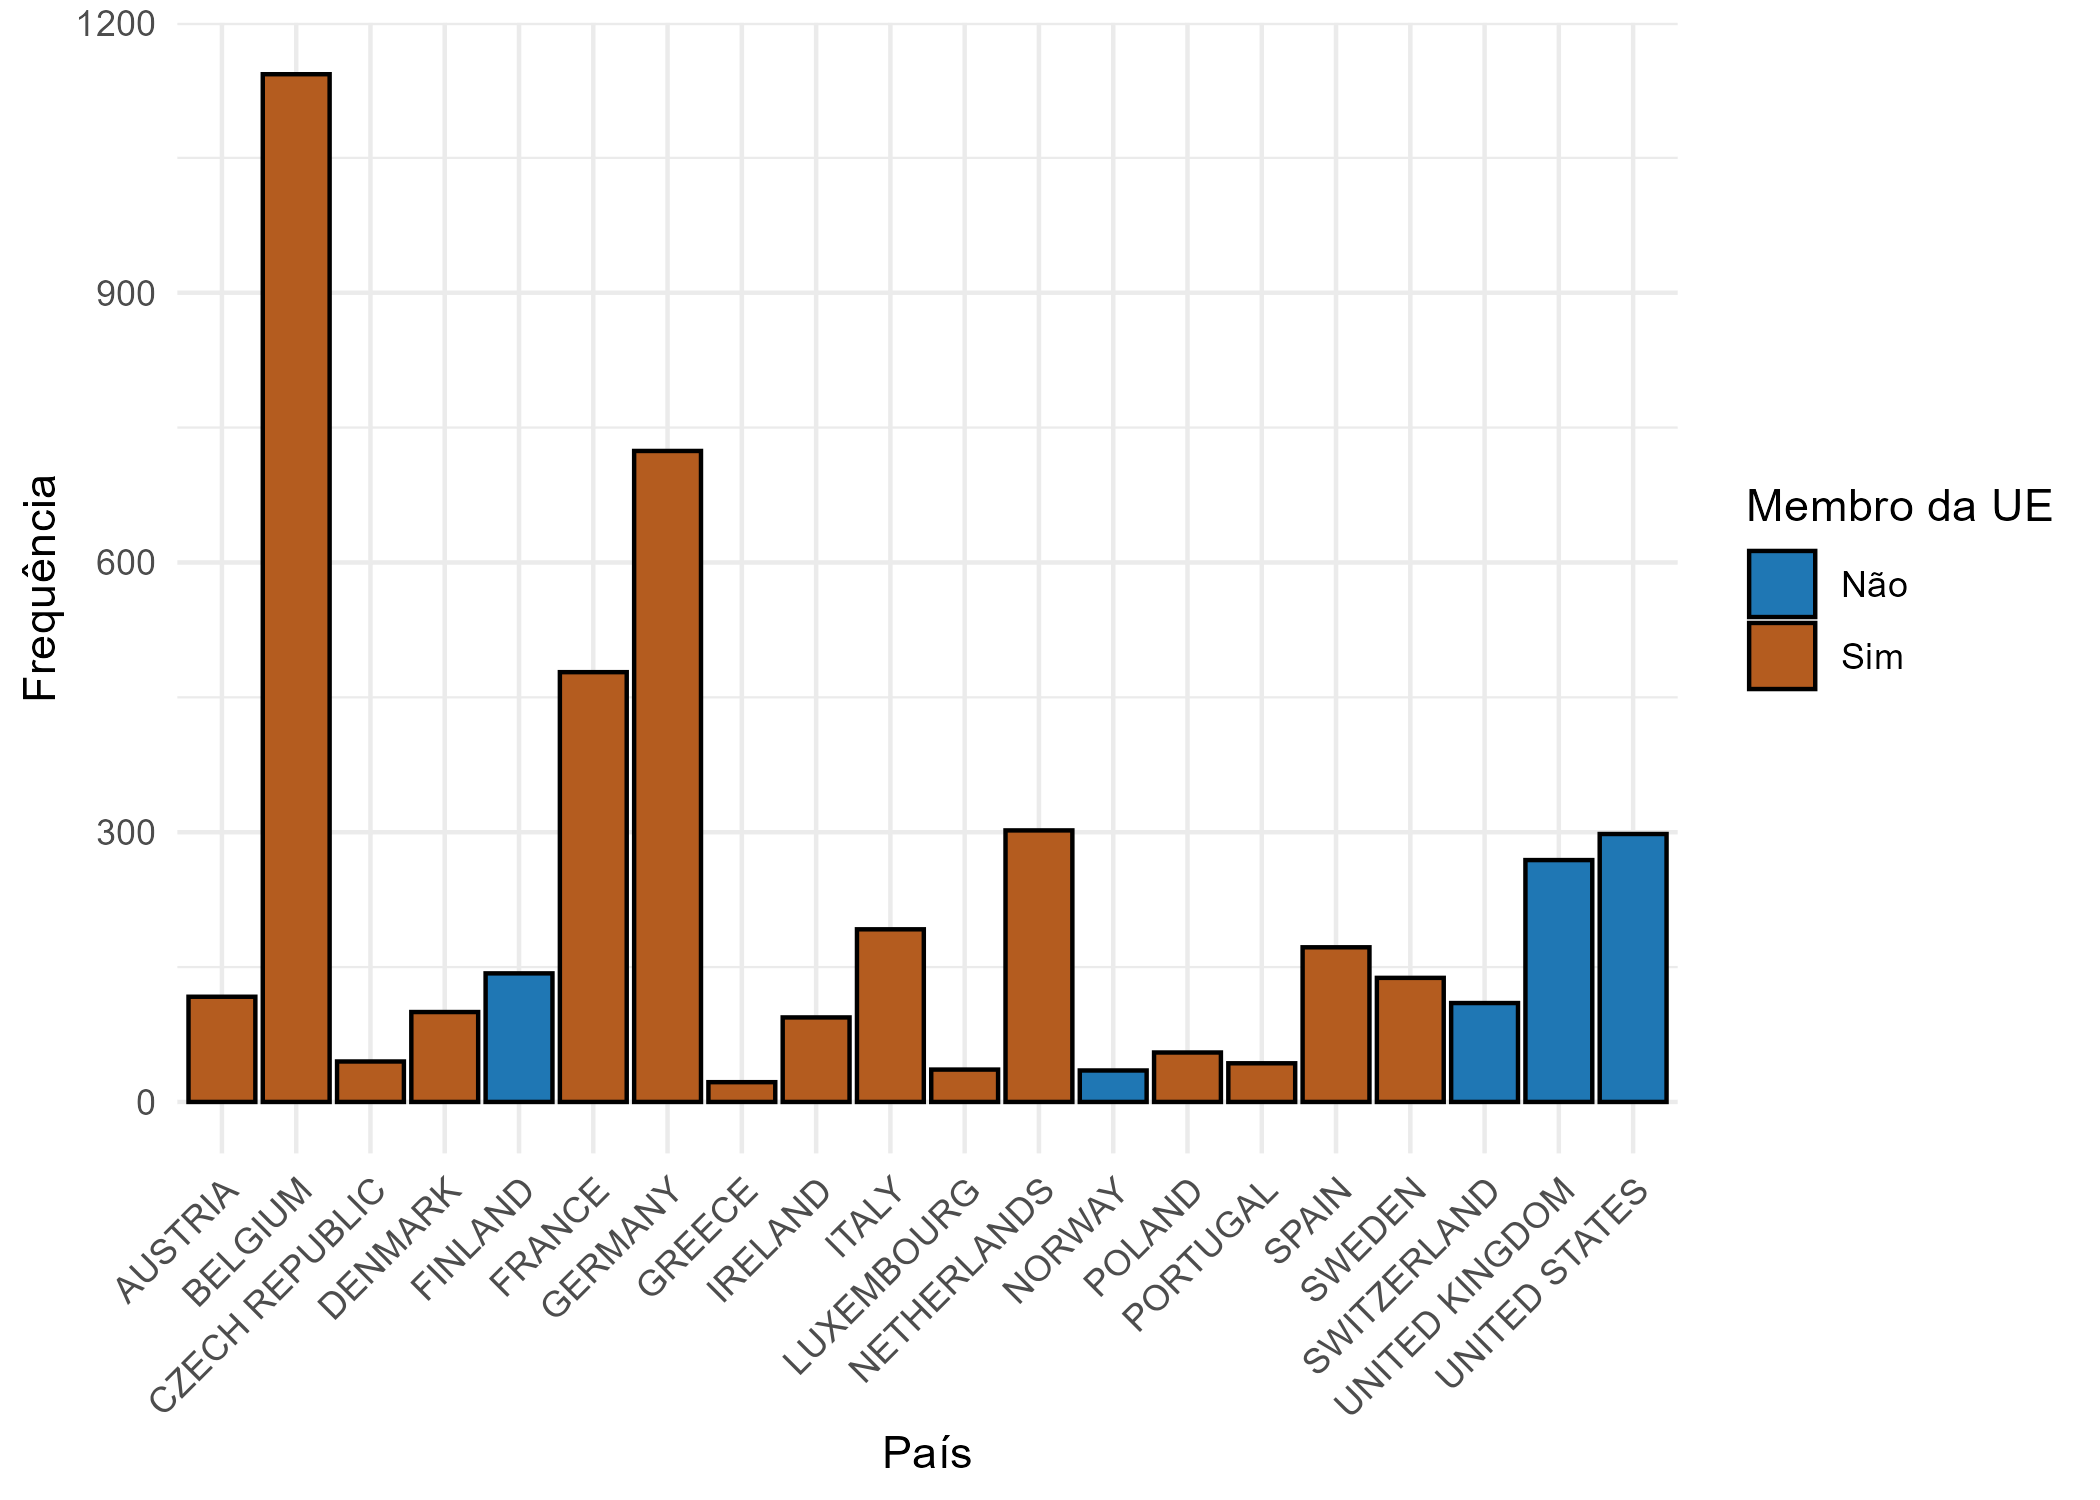
\includegraphics[width=0.9\textwidth]{figures/descriptives_lobbyists/barplot_country_distribution.png}
\caption{Top 20 países-sede (n = 4.516 organizações, totalizando 95,6\% do total de organizações)}
\label{fig:country_distribution}
\end{figure}

O fenômeno do \textit{venue-shopping} — a escolha estratégica do fórum mais favorável para exercer pressão — é central para entender essa distribuição \cite{kluver2015legislative}. A estrutura institucional da \acrshort{ue}, com poder decisório partilhado entre a Comissão, o Conselho e o Parlamento, incentiva os grupos de interesse a se estabelecerem nos locais onde podem monitorar e intervir mais eficazmente no ciclo político. A proeminência de países como Alemanha e França reflete não apenas a proximidade, mas também o peso político e econômico que exercem dentro da \acrshort{ue}.

Adicionalmente, a presença significativa de atores extracomunitários, que representam cerca de 20\% do total de organizações com sedes em 70 países (com destaque para os Estados Unidos, com 6,3\%), evidencia a importância da \acrshort{ue} como arena regulatória global. A atratividade do mercado europeu e o impacto de suas decisões incentivam atores internacionais a investir em uma presença local para influenciar a formulação de políticas que afetarão seus interesses. 

O recorte do top 20, que mostra uma cauda longa com muitos países de baixa frequência, reforça a ideia de que, embora o sistema seja permeável, os altos custos de manter uma operação de lobby eficaz na Europa centralizam a influência em atores com maiores recursos e localização estratégica.

% Distribuição temporal dos registros
Temporalmente, observa-se aceleração do registro de entidades após meados da década de 2010, com 2023 concentrando 17,9\% do total. Picos intermediários (2015--2016; 2020--2022) são compatíveis com ciclos legislativos, janelas regulatórias e alterações incrementais nos mecanismos de transparência.

\begin{figure}[!htbp]
\centering
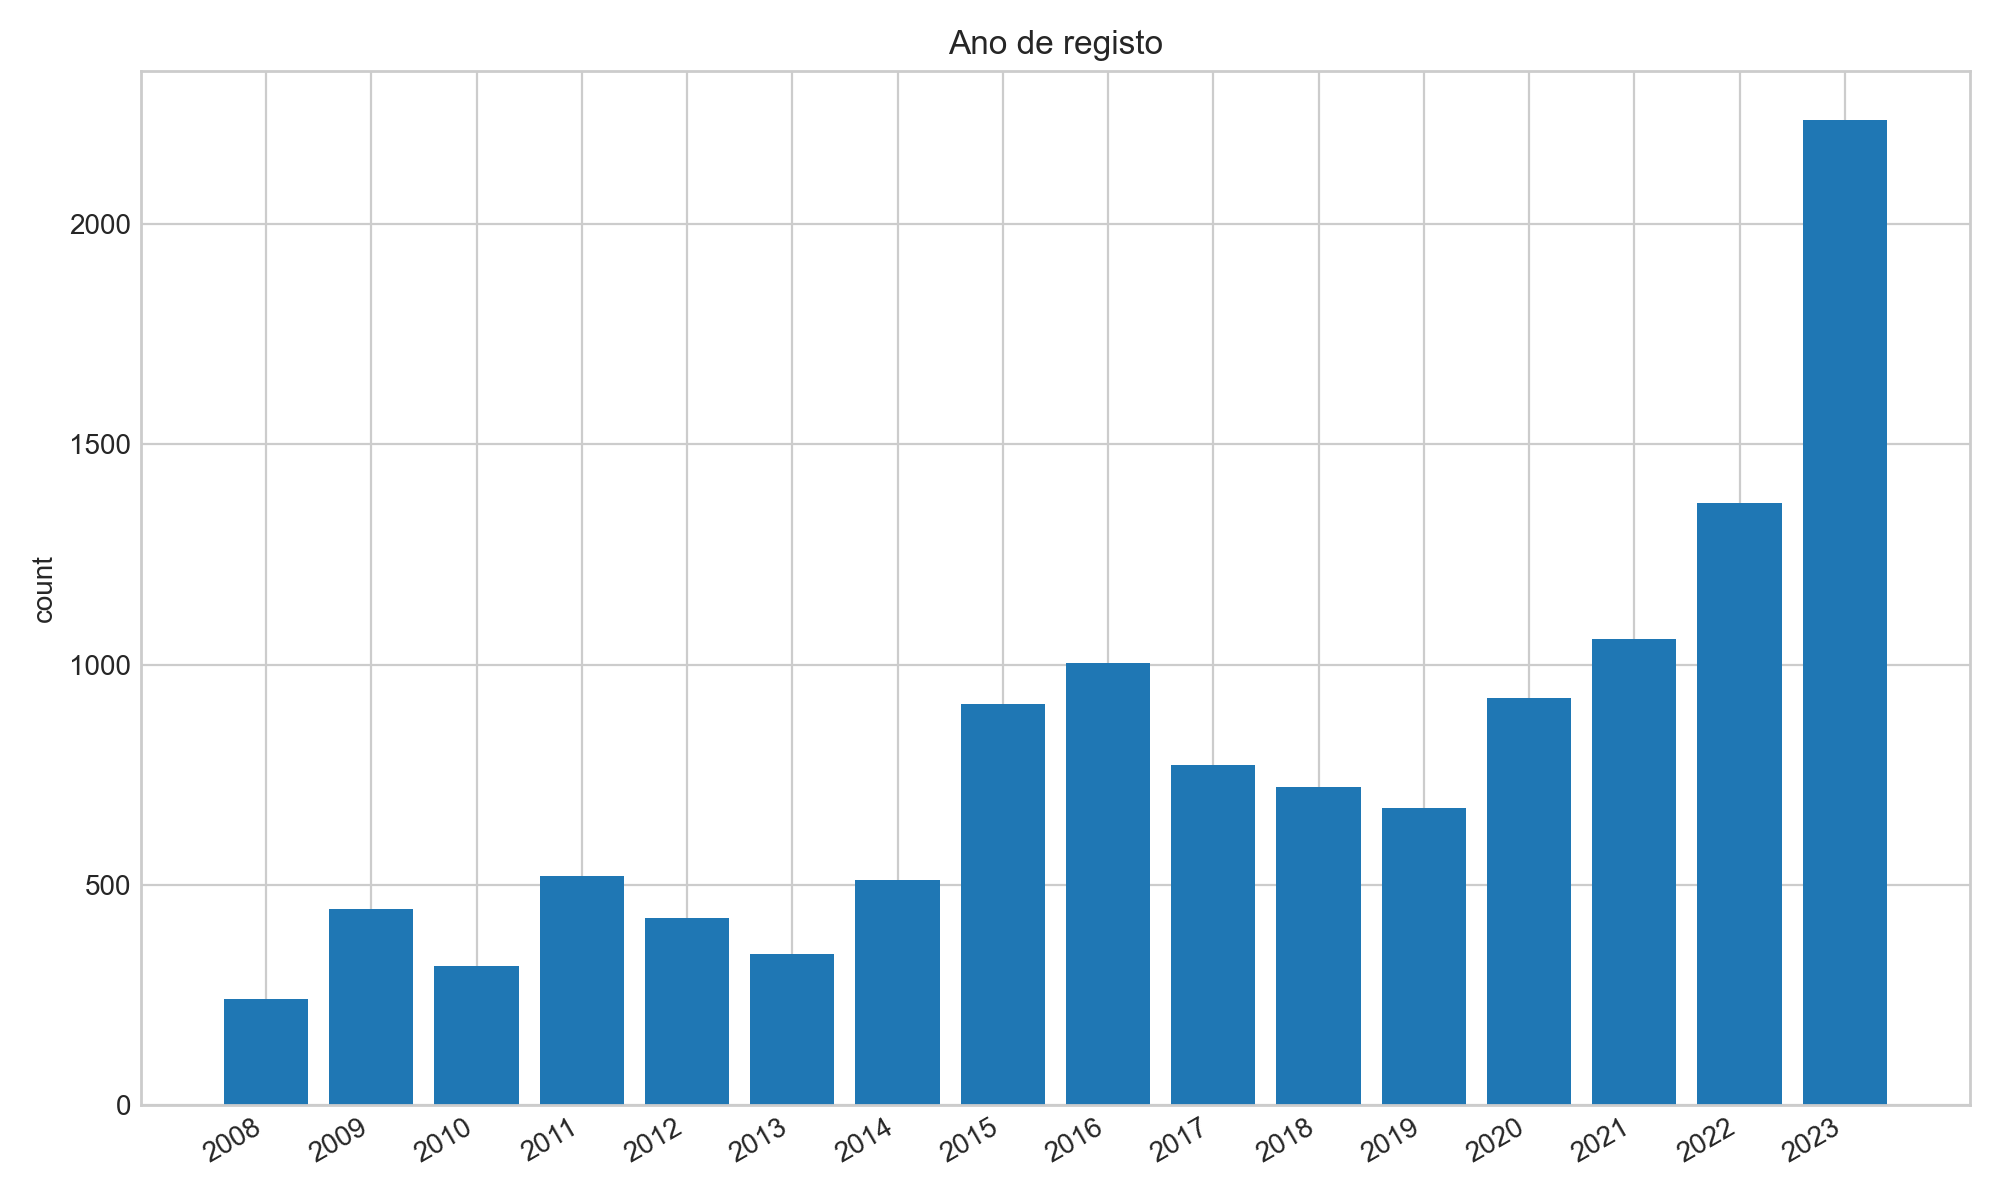
\includegraphics[width=0.75\textwidth]{figures/year_distribution.png}
\caption{Ano de registo}
\end{figure}

O padrão visual sugere crescimento estrutural recente do ecossistema de representação de interesses, possivelmente associado às agendas de transição digital e verde e à recomposição pós-pandemia.

% Distribuição temática
As incidências por domínio (Figura \ref{fig:theme_coverage}) destacam \textit{Economia e Comércio} (15\%), \textit{Tecnologia} (14,9\%) e \textit{Infraestrutura e Indústria} (14,4\%), seguidas por \textit{Tecnologia} (14,2\%) e \textit{Meio Ambiente e Clima} (13,8\%). Temas como \textit{Saúde} (9,8\%) e \textit{Educação} (8,1\%) são intermediários; \textit{Agricultura} (7,2\%) e \textit{Direitos Humanos} (6,2\%) têm menor incidência relativa.

\begin{figure}[!htbp]
\centering
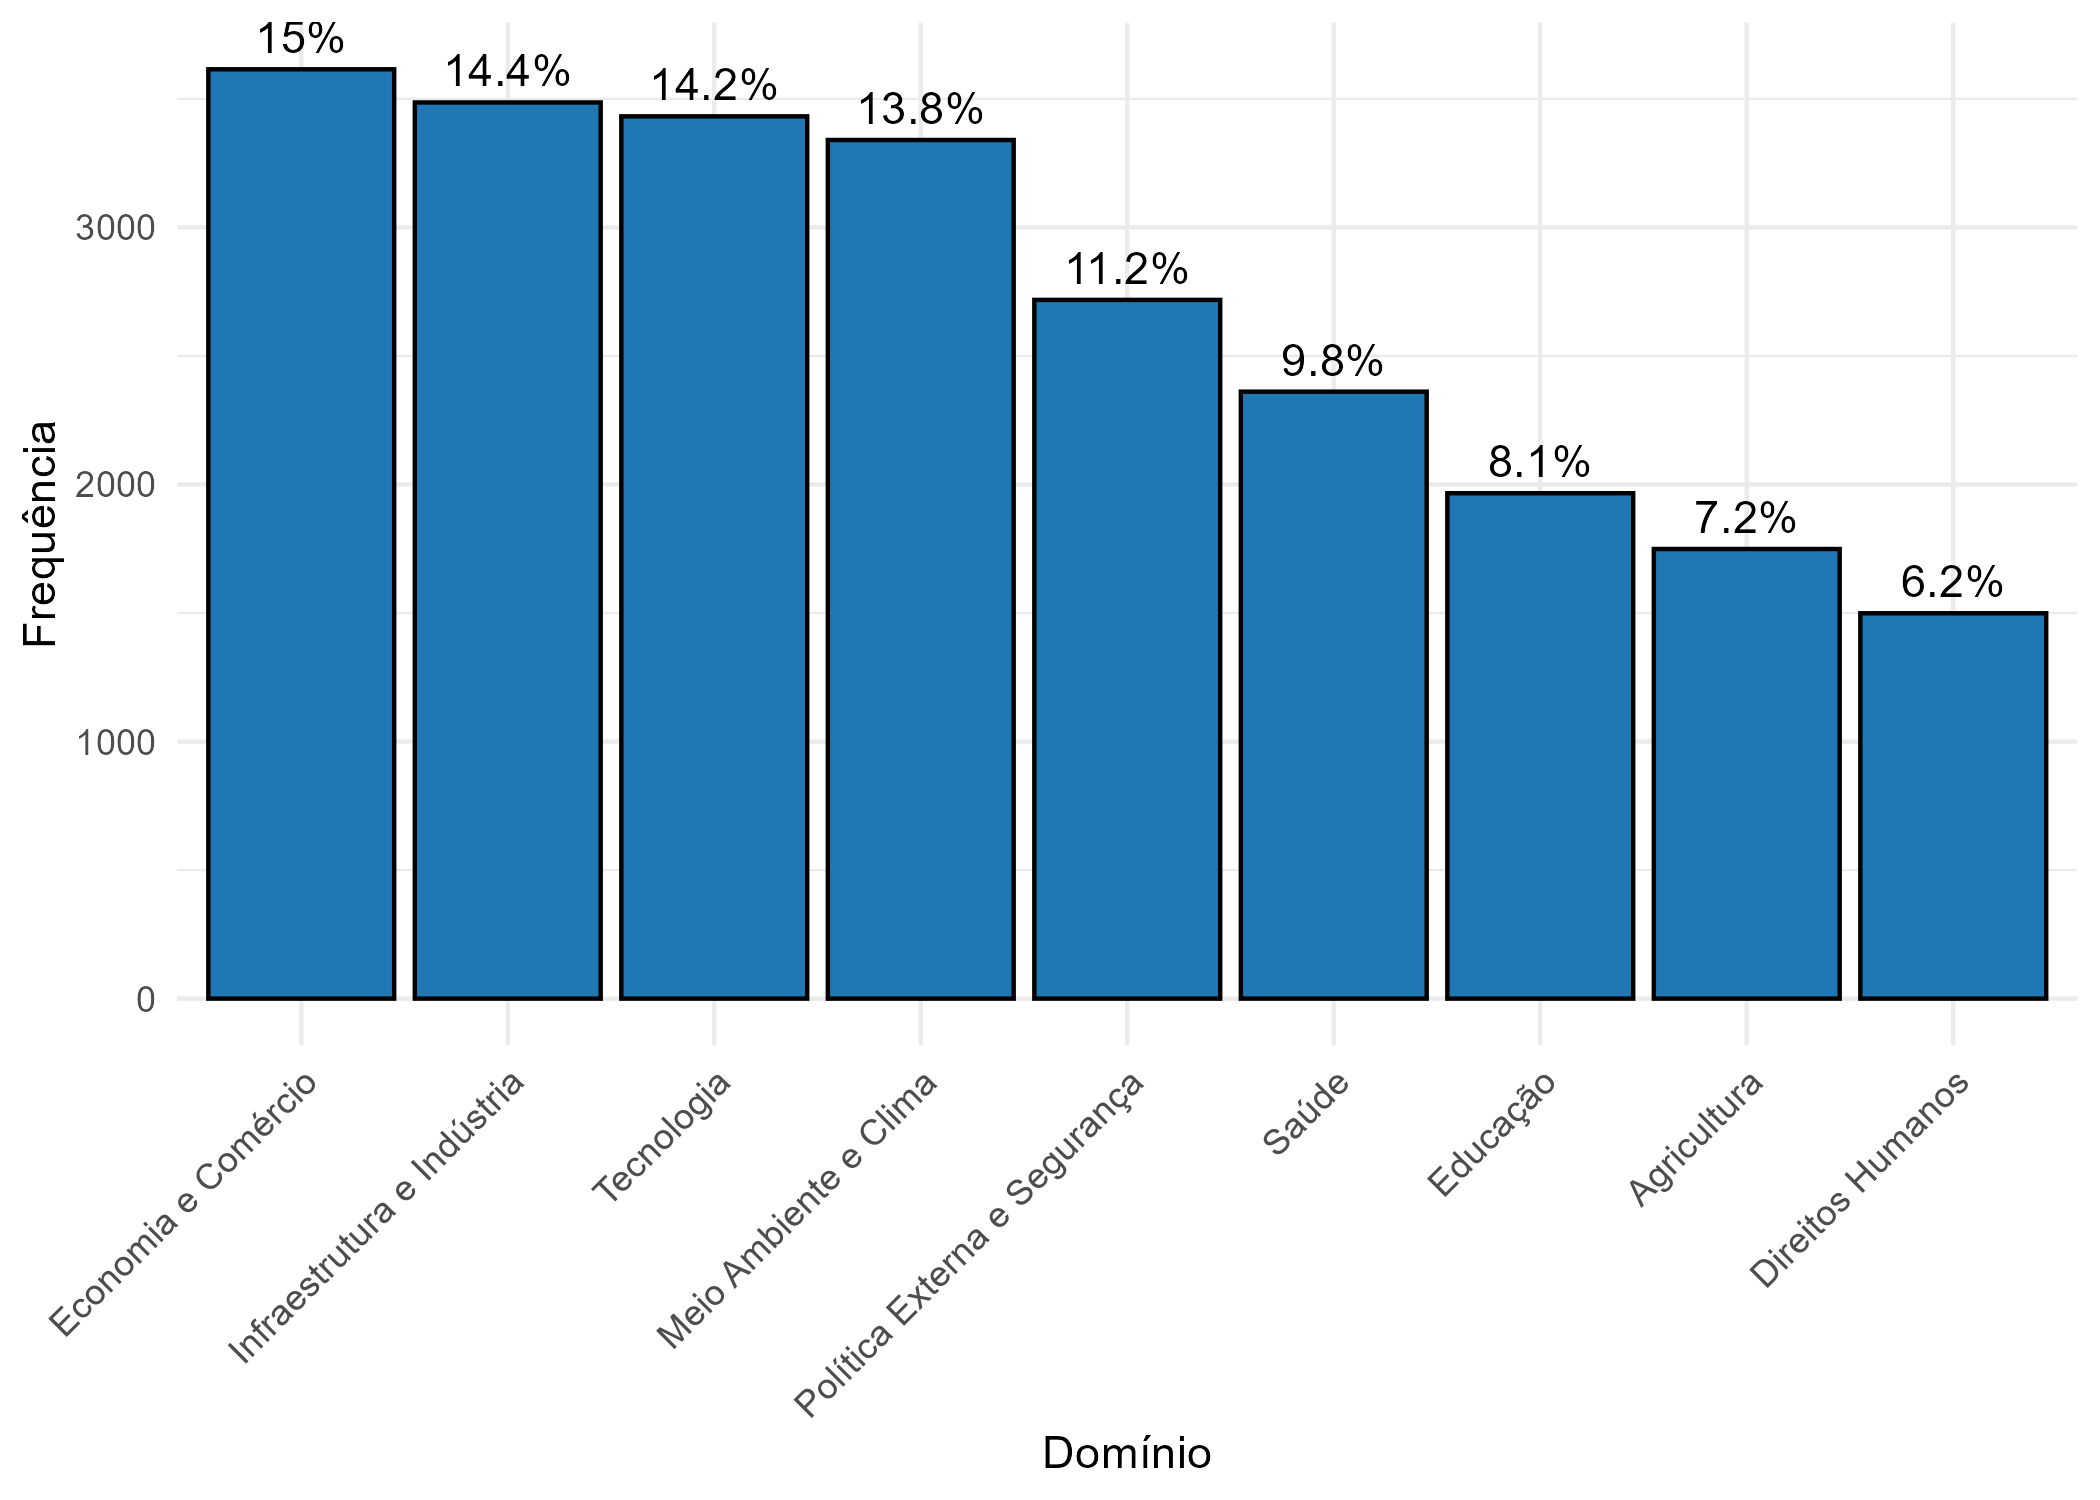
\includegraphics[width=0.9\textwidth]{figures/descriptives_lobbyists/barplot_domain_distribution.png}
\caption{Cobertura temática (proporção de entidades)}
\label{fig:theme_coverage}
\end{figure}

A distribuição temática (Figura \ref{fig:theme_coverage}) reflete uma concentração estratégica de esforços de lobby nas arenas de maior peso econômico e regulatório da União Europeia. A proeminência de domínios como "Economia e Comércio", "Infraestrutura e Indústria" e "Tecnologia" está alinhada com a literatura que demonstra uma correlação positiva entre a atividade de lobby e a saliência de um tema \cite{caldeira2000lobbying, baumgartner2010agendas}. São áreas onde as decisões políticas implicam altas consequências financeiras, mobilizando um volume expressivo de atores.

Adicionalmente, esses temas são caracterizados por uma elevada complexidade técnica. Este fator aumenta a demanda por informação especializada por parte dos decisores políticos, criando um vácuo que os lobistas buscam preencher para ganhar acesso e exercer influência, conforme sugere a literatura sobre o papel informacional do lobby \cite{kluver_informational_2012}. A própria agenda política da \acrshort{ue}, com iniciativas centrais como o Mercado Único Digital e o Pacto Ecológico Europeu, transforma esses domínios em focos de intensa atividade, corroborando a ideia de que os grupos de interesse são mais ativos nos temas em que o Estado também é mais atuante \cite{mahoney2008brussels}.

Em contraste, temas como "Direitos Humanos" e "Agricultura", embora relevantes, apresentam menor incidência relativa. Isso pode indicar que os interesses difusos ou setoriais dessas áreas enfrentam maiores desafios de ação coletiva ou utilizam estratégias de influência distintas, que não se refletem com a mesma intensidade no lobby direto. O padrão observado, portanto, sugere um ecossistema de lobby que responde de forma racional tanto aos incentivos econômicos quanto às necessidades informacionais geradas pela agenda regulatória da UE.

\begin{figure}[!htbp]
\centering
\includegraphics[width=0.75\textwidth]{figures/descriptives_lobbyists/histogram_themes_per_lobbyist.png}
\caption{Número de temas por lobista}
\label{fig:themes_per_lobbyist_hist}
\end{figure}

A análise da diversidade temática das organizações (Figura \ref{fig:themes_per_lobbyist_hist}) revela que a maioria dos lobistas atua em múltiplas frentes. A distribuição, que se assemelha a uma curva normal com média de 5,1 temas por organização, demonstra a coexistência de estratégias especializadas (focadas em poucos temas) e generalistas. Contudo, o padrão dominante é o de uma abordagem multi-temática, onde as organizações cobrem um portfólio de 3 a 7 áreas de interesse.

Este achado dialoga diretamente com o debate na literatura sobre os recursos mais valiosos para o lobby: expertise ("o que você sabe") versus conexões ("quem você conhece") \cite{bertrand2014whom}. A presença de atores especializados sugere uma aposta na expertise técnica como via de influência, especialmente em domínios de alta complexidade \cite{kluver_informational_2012}. Por outro lado, a predominância de atores multi-temáticos indica que uma estratégia mais ampla, possivelmente baseada em redes de contatos e na capacidade de adaptação a diferentes arenas políticas, é a norma no complexo ambiente institucional da \acrshort{ue}. A governança multinível e a interconexão de políticas na Europa podem incentivar as organizações a não se limitarem a um único nicho, buscando pontos de acesso em diferentes comissões e agências \cite{coen2019legislative}.

Em conjunto, os resultados descritivos apontam para um ecossistema plural, geograficamente ancorado em polos institucionais centrais, com dinamismo temporal recente e agendas orientadas por digitalização, competitividade industrial e sustentabilidade. Esses padrões informam as escolhas de especificação nos capítulos seguintes, notadamente a estratificação por perfis organizacionais, a construção de domínios temáticos e o controle para tendências temporais.


Os resultados descritivos delineiam um panorama abrangente do universo de lobistas registados junto às instituições europeias. Em primeiro lugar, a distribuição por categoria revela a coexistência de diferentes perfis organizacionais (\textit{Empresas}, \textit{\acrshort{ong}s} e \textit{Outros}), com magnitudes comparáveis entre atores empresariais e organizações da sociedade civil. Essa composição é compatível com a literatura sobre pluralismo organizacional e competição por acesso institucional no contexto da \acrshort{ue}, sugerindo um campo de ação onde interesses difusos e concentrados buscam simultaneamente agenda e influência.

Em síntese, as evidências descritivas apontam para um ecossistema plural, geograficamente ancorado em polos institucionais centrais, com dinamismo temporal recente e agendas orientadas por digitalização, competitividade industrial e sustentabilidade. Esses padrões informam as escolhas de especificação nos capítulos seguintes, notadamente a estratificação por perfis organizacionais, a construção de domínios temáticos e o controle para tendências temporais.


\section{Análise descritiva do tratamento}
\label{sec:resultados_descritica}

Esta seção apresenta uma análise descritiva sistemática dos dados utilizados para investigar os efeitos do lobbying na atividade parlamentar dos deputados do Parlamento Europeu. A abordagem adotada segue uma estratégia analítica multinível, iniciando com padrões agregados gerais e progredindo para análises desagregadas mais específicas. Esta progressão metodológica permite compreender tanto as tendências globais quanto os mecanismos específicos que operam no nível individual e temporal.

O conjunto de dados constitui um painel balanceado que combina informações sobre atividade parlamentar (perguntas) e intensidade de lobbying (reuniões) para 1.353 deputados ao longo de 63 meses, de julho de 2019 a novembro de 2024 em 9 domínios de política pública. Esta estrutura temporal permite capturar variações tanto na dimensão \textit{cross-sectional} (entre deputados e domínios) quanto longitudinal (evolução temporal), fornecendo a base empírica necessária para estratégias de identificação causal robustas.

Considerando a unidade de análise a tríade MEP-domínio-mês, temos 767.151 observações com taxa de completude de 100\%. Esta estrutura balanceada é metodologicamente vantajosa, pois elimina preocupações com viés de seleção decorrente de atrito amostral e garante que as estimativas não sejam distorcidas por padrões de observações ausentes.

A cobertura temporal de julho de 2019 a novembro de 2024 é particularmente relevante por abranger períodos de intensa atividade legislativa europeia, incluindo a transição entre legislaturas e eventos político-econômicos significativos. Destaca-se, nesse intervalo, o impacto da pandemia de COVID-19, que afetou profundamente tanto a dinâmica da atividade parlamentar quanto as estratégias de lobbying. A pandemia resultou em mudanças substanciais nos modos de trabalho do Parlamento Europeu, com a adoção de sessões remotas e restrições a reuniões presenciais, o que pode ter alterado padrões de interação entre deputados e grupos de interesse. Assim, a análise cobre não apenas períodos de normalidade institucional, mas também um contexto de crise sanitária global, permitindo investigar como choques exógenos desse tipo influenciam o comportamento político e o lobbying.

A \autoref{fig:time_series} apresenta a evolução temporal das variáveis principais no nível mais agregado, revelando padrões que são fundamentais para compreender a dinâmica do sistema político europeu ao longo do período estudado.

\begin{figure}[htbp]
\centering
\includegraphics[width=\textwidth]{figures/fig1_time_series_meetings_questions.pdf}
\caption{Evolução temporal da atividade parlamentar e de lobbying}
\label{fig:time_series}
% \note{O painel superior esquerdo mostra os totais mensais agregados de perguntas e reuniões. O painel superior direito apresenta as médias mensais por observação MEP-domínio. O painel inferior esquerdo mostra a evolução da proporção de observações com atividade de lobbying. O painel inferior direito apresenta a estabilidade da correlação contemporânea entre as variáveis ao longo do tempo.}
\end{figure}

A análise temporal revela quatro padrões empiricamente relevantes. Primeiro, observa-se uma \textbf{tendência crescente} em ambas as variáveis ao longo do período, sugerindo intensificação tanto da atividade parlamentar quanto do lobbying. Segundo, existe clara \textbf{sazonalidade} relacionada ao calendário parlamentar, com reduções sistemáticas durante períodos de recesso. Terceiro, identificam-se \textbf{picos de atividade} que coincidem com discussões de legislação relevante em domínios específicos, indicando resposta coordenada do sistema político. Quarto, a \textbf{correlação contemporânea} entre perguntas e reuniões permanece relativamente estável ao longo do tempo, sugerindo estabilidade estrutural na relação entre as variáveis.

% não há exatamente essa tendência cerescente...


Estes padrões temporais têm implicações metodológicas importantes. A presença de tendências temporais justifica a inclusão de efeitos fixos de tempo nas especificações econométricas para controlar choques temporais comuns. A sazonalidade observada valida a escolha da frequência mensal como unidade temporal, capturando variações de curto prazo sem introduzir ruído excessivo. A estabilidade da correlação fornece evidência preliminar contra quebras estruturais que poderiam comprometer a validade das estimativas.

% \subsection{Padrões de participação: análise agregada por deputado}

Complementando a análise temporal, é fundamental examinar os padrões de participação no nível individual dos deputados. Esta perspectiva agregada revela a distribuição da atividade de lobbying entre os parlamentares e fornece insights sobre a concentração e heterogeneidade dos fenômenos estudados.



As \autoref{fig:proportion_meetings}, \autoref{fig:correlation_meetings_questions} e \autoref{fig:meetings_hist} apresentam uma análise dos padrões de participação agregados por deputado, revelando aspectos da distribuição da atividade de lobbying no Parlamento Europeu que impactam a identificação causal.

% \begin{figure}[htbp]
% \centering
% \includegraphics[width=\textwidth]{figures/fig6_mep_aggregated_analysis.pdf}
% \caption{Análise agregada por MEP: distribuição e intensidade do tratamento}
% \label{fig:mep_aggregated}
% \note{O painel superior esquerdo mostra a proporção de deputados que receberam pelo menos uma reunião de lobbying durante todo o período. O painel superior direito apresenta a distribuição da intensidade total de reuniões entre deputados tratados. O painel inferior esquerdo examina a relação agregada entre reuniões e perguntas totais por deputado. O painel inferior direito identifica os deputados mais ativos em termos de recepção de lobbying.}
% \end{figure}



% \subsubsection{Distribuição do tratamento entre deputados}

\begin{figure}[htbp]
    \centering
    \includegraphics[width=\textwidth]{figures/fig2_proportion_meetings.pdf}
    \caption{Evolução temporal da proporção de \acrshort{mpe}s que participaram de reuniões de lobbying}
    \label{fig:proportion_meetings}
    % \note{O painel superior esquerdo mostra os totais mensais agregados de perguntas e reuniões. O painel superior direito apresenta as médias mensais por observação MEP-domínio. O painel inferior esquerdo mostra a evolução da proporção de observações com atividade de lobbying. O painel inferior direito apresenta a estabilidade da correlação contemporânea entre as variáveis ao longo do tempo.}
\end{figure}

\begin{figure}[htbp]
    \centering
    \includegraphics[width=\textwidth]{figures/fig3_correlation_meetings_questions.pdf}
    \caption{Evolução temporal da correlação entre reuniões e perguntas}
    \label{fig:correlation_meetings_questions}
    % \note{O painel superior esquerdo mostra os totais mensais agregados de perguntas e reuniões. O painel superior direito apresenta as médias mensais por observação MEP-domínio. O painel inferior esquerdo mostra a evolução da proporção de observações com atividade de lobbying. O painel inferior direito apresenta a estabilidade da correlação contemporânea entre as variáveis ao longo do tempo.}
\end{figure}

\begin{figure}[htbp]
    \centering
    \includegraphics[width=\textwidth]{figures/fig3.1_meetings_hist.pdf}
    \caption{Distribuição de reuniões por \acrshort{mpe}}
    \label{fig:meetings_hist}
    % \note{O painel superior esquerdo mostra os totais mensais agregados de perguntas e reuniões. O painel superior direito apresenta as médias mensais por observação MEP-domínio. O painel inferior esquerdo mostra a evolução da proporção de observações com atividade de lobbying. O painel inferior direito apresenta a estabilidade da correlação contemporânea entre as variáveis ao longo do tempo.}
\end{figure}


A análise revela três características fundamentais da distribuição de tratamento. Primeiro, existe \textbf{participação substancial mas não universal}: 46,3\% dos deputados (637 de 1.353) receberam pelo menos uma reunião de lobbying durante o período estudado. Esta proporção indica que o lobbying é um fenômeno disseminado mas não ubíquo no sistema parlamentar europeu.

Segundo, observa-se \textbf{concentração extrema} na intensidade de tratamento. Entre os deputados que receberam lobbying, a distribuição é altamente assimétrica: enquanto a mediana é de 105 reuniões por deputado, a média é de 288,2 reuniões, indicando que uma minoria de parlamentares concentra uma proporção desproporcional da atividade lobista. O caso extremo de um deputado com 4.274 reuniões ilustra esta concentração.

Terceiro, a \textbf{correlação agregada} entre reuniões e perguntas totais por deputado é surpreendentemente baixa (0,056), contrastando com correlações mais elevadas observadas no nível temporal. Este padrão sugere que os efeitos do lobbying podem ser mais evidentes em frequências temporais específicas do que em padrões de atividade agregados de longo prazo.

% \paragraph{Implicações para a estratégia empírica}

Estes padrões agregados têm implicações importantes para a identificação causal. A concentração do tratamento em uma minoria de deputados sugere que estratégias de identificação baseadas em variação cross-sectional podem sofrer de poder estatístico limitado. Simultaneamente, a variação substancial na intensidade de tratamento entre deputados tratados fornece fonte valiosa de identificação para estimativas de dose-resposta.

A baixa correlação agregada, combinada com correlações temporais mais elevadas, indica que a identificação causal pode beneficiar-se de estratégias que explorem variação temporal within-individual rather than cross-sectional between-individual. Esta evidência preliminar orienta a especificação de modelos com efeitos fixos de deputado para controlar heterogeneidade não observada time-invariant.

\begin{table}[htbp]
\centering
\caption{Estatísticas agregadas de tratamento por deputado}
\label{tab:mep_treatment_stats}
\begin{tabular}{lr}
\toprule
\textbf{Estatística} & \textbf{Valor} \\
\midrule
Total de deputados únicos & 1{,}353 \\
Deputados que receberam tratamento & 627 \\
Taxa de tratamento por deputado (\%) & 46{,}3\% \\
\midrule
\textbf{Entre deputados tratados:} & \\
Reuniões médias por deputado & 288{,}2 \\
Reuniões medianas por deputado & 105{,}0 \\
Desvio padrão & 468{,}9 \\
Deputado mais ativo (reuniões) & 4{,}274 \\
\midrule
\textbf{Correlação agregada:} & \\
Correlação reuniões-perguntas & 0{,}056 \\
\bottomrule
\end{tabular}
\end{table}

\subsection{Heterogeneidade entre domínios de política pública}

A terceira dimensão da análise agregada examina a variação entre domínios de política pública. Esta heterogeneidade setorial é teoricamente relevante porque diferentes áreas de política podem apresentar características distintas em termos de complexidade técnica, interesse econômico e organização de grupos de pressão, afetando tanto a demanda por lobbying quanto a responsividade parlamentar.

% \paragraph{Padrões de tratamento por domínio}

A \autoref{fig:domain_treatment} apresenta uma análise sistemática da variação inter-domínios em múltiplas dimensões: penetração, volume e intensidade do tratamento, bem como padrões temporais de iniciação.


\begin{table}[htbp]
    \centering
    \caption{Taxa de tratamento por domínio: deputados únicos que receberam lobbying}
    \label{tab:domain_treatment_rates}
    \begin{tabular}{lrrr}
    \toprule
    \textbf{Domínio} & \textbf{Deputados Tratados} & \textbf{Total Deputados} & \textbf{Taxa (\%)} \\
    \midrule
    Economia e Comércio & 615 & 1{,}353 & 45{,}5 \\
    Tecnologia & 615 & 1{,}353 & 45{,}5 \\
    Política Externa e Segurança & 611 & 1{,}353 & 45{,}2 \\
    Infraestrutura e Indústria & 610 & 1{,}353 & 45{,}1 \\
    Meio Ambiente e Clima & 607 & 1{,}353 & 44{,}9 \\
    Saúde & 599 & 1{,}353 & 44{,}3 \\
    Educação & 578 & 1{,}353 & 42{,}7 \\
    Direitos Humanos & 564 & 1{,}353 & 41{,}7 \\
    Agricultura & 554 & 1{,}353 & 40{,}9 \\
    \bottomrule
    \end{tabular}
    \end{table}

A análise revela heterogeneidade sistemática mas moderada entre domínios. Em termos de \textbf{penetração}, as taxas variam de 40,9\% (agricultura) a 45,5\% (economia e tecnologia), uma amplitude de apenas 4,6 pontos percentuais. Esta variação relativamente pequena sugere que o lobbying possui caráter transversal, não concentrando-se drasticamente em setores específicos.

Contudo, emergem padrões teoricamente consistentes. Domínios relacionados à \textbf{regulação econômica} (economia e comércio, tecnologia, infraestrutura) apresentam sistematicamente maiores taxas de penetração, refletindo os elevados interesses econômicos e a complexidade regulatória que incentivam investimento em atividades de lobbying. Este padrão é especialmente relevante considerando que a promoção da integração econômica é o foco principal de um bloco como a União Europeia, o que naturalmente direciona maior atenção e mobilização de grupos de interesse para essas áreas. Inversamente, domínios com características de bem público (agricultura, direitos humanos) apresentam menores taxas, consistente com problemas de ação coletiva e menor capacidade organizacional de grupos difusos.


\begin{figure}[htbp]
    \centering
    \includegraphics[width=\textwidth]{figures/fig7_domain_treatment_analysis.pdf}
    \caption{Análise detalhada de tratamento por domínio de política pública}
    \label{fig:domain_treatment}
    \note{O painel superior esquerdo mostra a taxa de penetração (percentual de deputados únicos que receberam pelo menos uma reunião em cada domínio). O painel superior direito apresenta o volume absoluto de deputados tratados. O painel inferior esquerdo mostra a intensidade média condicional de tratamento. O painel inferior direito apresenta a evolução temporal dos primeiros tratamentos para os três domínios mais ativos.}
\end{figure}


A heterogeneidade observada entre domínios tem duas implicações metodológicas importantes. Primeiro, a variação sistemática sugere que estimativas de efeito médio podem mascarar diferenças substantivas entre setores, justificando análises de heterogeneidade de efeitos por domínio. Segundo, a ordenação consistente dos domínios por múltiplas métricas (penetração, volume, intensidade) sugere que esta heterogeneidade reflete características estruturais dos setores ao invés de variação aleatória, aumentando a credibilidade de interpretações causais diferenciadas.

% \begin{figure}[htbp]
% \centering
% \includegraphics[width=.9\textwidth]{figures/fig3_domain_heterogeneity.pdf}
% \caption{Heterogeneidade por domínio: atividade média e distribuições}
% \label{fig:domain_heterogeneity}
% \note{O painel superior esquerdo mostra a atividade média mensal por domínio para ambas as variáveis. O painel superior direito apresenta as taxas de tratamento mensais. Os painéis inferiores mostram box plots das distribuições completas por domínio, evidenciando tanto diferenças de localização quanto de dispersão entre áreas de política pública.}
% \end{figure}

% \subsection{Análise detalhada: observações MEP-domínio-período}

% Após estabelecer os padrões agregados gerais, temporais e setoriais, esta seção examina as características específicas dos dados no nível mais desagregado: observações MEP-domínio-mês. Esta análise é crucial porque a unidade de observação constitui a base para as estimações econométricas e suas características distribucionais determinam as escolhas metodológicas apropriadas.

% \paragraph{Especialização temática e o problema da inflação artificial de zeros}

A análise da inflação de zeros requer cuidado metodológico particular, pois a unidade de observação MEP-domínio-mês pode gerar inflação \textbf{artificial} de zeros. Como documentado na literatura sobre comportamento parlamentar \cite{example}, deputados tendem a especializar-se tematicamente, concentrando atividade em subconjuntos específicos de domínios. Consequentemente, grupos de interesse, cientes desta especialização, direcionam esforços de lobbying apenas para deputados ativos em suas áreas de interesse.

\textbf{Evidência de especialização temática:} A análise da atividade parlamentar agregada por deputado revela que 97,6\% dos MEPs são \textbf{generalistas} (Índice Herfindahl < 0,4), atuando em média em 7,47 dos 9 domínios disponíveis. Contudo, identificam-se 22 MEPs altamente especializados (HHI > 0,8) que concentram perguntas em domínios únicos, e 26 moderadamente especializados (HHI 0,4-0,8), demonstrando que a especialização, embora limitada, é empiricamente relevante.

\paragraph{Análise corrigida da inflação de zeros}

Para evitar viés na interpretação, a análise da inflação de zeros deve considerar níveis de agregação teoricamente apropriados. A \autoref{tab:zero_inflation_comparison} apresenta uma comparação sistemática entre diferentes níveis de agregação.

\begin{table}[htbp]
\centering
\caption{Inflação de zeros por nível de agregação}
\label{tab:zero_inflation_comparison}
% Usar tabularx para permitir quebra de linha na primeira coluna e evitar overfull hbox
\begin{tabularx}{\textwidth}{>{\raggedright\arraybackslash}X r r r}
\toprule
\textbf{Nível de Agregação} & \textbf{Observações} & \textbf{Zeros Perguntas} & \textbf{Zeros Reuniões} \\
\midrule
MEP-Domínio-Mês (original) & 767{.}151 & 92{,}2\% & 92{,}5\% \\
MEP-Mês (domínios ativos) & 54{.}117 & 70{,}9\% & 85{,}2\% \\
Domínio-Mês (agregado) & 567 & 3{,}2\% & 0{,}0\% \\
\bottomrule
\end{tabularx}
\end{table}

Os resultados revelam que a inflação de zeros é \textbf{sensível ao nível de agregação} e parcialmente \textbf{artificial} quando consideramos especializações temáticas:

\begin{enumerate}
    \item \textbf{Nível MEP-domínio-mês}: A inflação aparentemente extrema (>92\%) reflete em grande parte combinações MEP-domínio onde não se espera atividade sistemática devido à especialização.
    
    \item \textbf{Nível MEP-mês} (agregando apenas domínios onde o MEP demonstra atividade parlamentar): A inflação reduz substancialmente para 70,9\% (perguntas) e 85,2\% (reuniões), revelando que a atividade é \textit{episódica} mas não \textit{ausente}.
    
    \item \textbf{Nível domínio-mês} (agregando todos os MEPs ativos): A inflação torna-se negligível (3,2\% para perguntas, 0\% para reuniões), indicando que há atividade consistente em todos os domínios quando consideramos o conjunto de deputados relevantes.
\end{enumerate}

% A \autoref{fig:corrected_zero_inflation} apresenta uma comparação visual sistemática entre os diferentes níveis de agregação, evidenciando como a especialização temática afeta a interpretação da inflação de zeros.

% \begin{figure}[htbp]
% \centering
% \includegraphics[width=\textwidth]{figures/fig_corrected_zero_inflation_analysis.pdf}
% \caption{Análise corrigida da inflação de zeros considerando especialização temática}
% \label{fig:corrected_zero_inflation}
% \note{O painel superior esquerdo mostra a inflação aparente no nível MEP-domínio-mês original. O painel superior direito apresenta a inflação corrigida no nível MEP-mês considerando apenas domínios ativos. O painel inferior esquerdo mostra a distribuição de especialização temática dos MEPs. O painel inferior direito compara a evolução temporal dos totais mensais entre os métodos original e corrigido.}
% \end{figure}

% \paragraph{Implicações metodológicas revisadas}

Esta análise corrigida tem implicações fundamentais para a estratégia econométrica:

\begin{enumerate}
    \item \textbf{Falso problema de inflação de zeros}: A aparente inflação extrema (>92\%) é em grande parte \textbf{artificial}, resultante da inclusão de combinações MEP-domínio teoricamente implausíveis. A inflação \textbf{real} no nível MEP-mês é substancialmente menor (70,9\%-85,2\%).
    
    \item \textbf{Justificativa para efeitos fixos}: A especialização temática documentada justifica ainda mais fortemente o uso de efeitos fixos MEP×domínio, pois captura heterogeneidade não observada na propensão à atividade em áreas específicas.
    
    \item \textbf{Modelos econométricos apropriados}: Enquanto a inflação moderada (70,9\%) ainda sugere benefícios de modelos de contagem (PPML), a inflação não é tão extrema a ponto de requerer modelos zero-inflated especializados.
    
    \item \textbf{Unidade de análise}: A evidência sustenta a escolha da unidade MEP-domínio-mês para análise causal, pois captura a granularidade necessária para identificação, desde que acompanhada de controles apropriados para especialização.
    
    \item \textbf{Interpretação de resultados}: Efeitos estimados devem ser interpretados condicionalmente à especialização temática, com atenção particular às margens extensiva (entrada em novos domínios) versus intensiva (aumento de atividade em domínios existentes).
\end{enumerate}

% \paragraph{Decomposição em margens extensiva e intensiva}

% A extrema inflação de zeros torna analiticamente vantajoso decompor o fenômeno em duas margens conceituais distintas: a \textbf{margem extensiva} (decisão de participar) e a \textbf{margem intensiva} (nível de atividade condicional à participação). Esta decomposição é teoricamente relevante porque diferentes mecanismos causais podem operar em cada margem.

% A \autoref{fig:extensive_intensive} apresenta uma análise detalhada desta decomposição, incluindo a sobreposição entre atividades parlamentares e de lobbying.

% \begin{figure}[htbp]
% \centering
% \includegraphics[width=\textwidth]{figures/fig5_extensive_intensive_margins.pdf}
% \caption{Análise das margens extensiva e intensiva}
% \label{fig:extensive_intensive}
% \note{O painel superior esquerdo apresenta a tabulação cruzada entre atividade parlamentar e de lobbying, revelando padrões de sobreposição. O painel superior direito decompõe as margens extensiva (participação) e intensiva (intensidade condicional). Os painéis inferiores mostram as distribuições condicionais completas para ambas as variáveis na margem intensiva.}
% \end{figure}

% A tabulação cruzada revela um padrão notável: apenas \textbf{0,4\%} das observações apresentam simultaneamente perguntas parlamentares e reuniões de lobbying. Esta baixa sobreposição indica que atividade parlamentar e lobbying são largamente \textbf{independentes} no nível temporal mensal, sugerindo que potenciais efeitos causais podem operar através de canais indiretos ou com defasagens temporais que não são captadas na correlação contemporânea.

% Na margem extensiva, 7,8\% das observações apresentam atividade parlamentar e 7,5\% apresentam atividade de lobbying. Na margem intensiva, condicionalmente à participação, as médias são 1,54 perguntas e 3,15 reuniões por observação, com distribuições altamente assimétricas evidenciando concentração mesmo dentro do subconjunto de observações ativas.

% \paragraph{Correlações e relações entre variáveis}

% Para completar a caracterização dos dados, a \autoref{fig:correlation_analysis} examina as relações diretas entre as variáveis principais através de múltiplas perspectivas analíticas.

% \begin{figure}[htbp]
% \centering
% \includegraphics[width=\textwidth]{figures/fig4_correlation_analysis.pdf}
% \caption{Análise de correlações e relações entre variáveis}
% \label{fig:correlation_analysis}
% \note{O painel superior esquerdo mostra a relação geral entre perguntas e reuniões no nível MEP-domínio-mês. O painel superior direito apresenta a mesma relação em escala logarítmica. O painel inferior esquerdo mostra as correlações por domínio. O painel inferior direito apresenta a matriz de correlação entre as variáveis principais.}
% \end{figure}

% A análise de correlações revela padrões consistentes com a baixa sobreposição contemporânea observada anteriormente. No nível agregado MEP-domínio-mês, a correlação é positiva mas modesta. Interessantemente, existe heterogeneidade sistemática nas correlações entre domínios, sugerindo que a força da relação varia com características setoriais específicas.

\subsection{Síntese e implicações metodológicas}

A análise descritiva multinível revela um conjunto coerente de \textit{stylized facts} que informam tanto a compreensão teórica quanto as escolhas metodológicas para a análise causal subsequente.

% \paragraph{Características empíricas principais}

Primeiro, o \textbf{lobbying é um fenômeno disseminado mas episódico}. Enquanto 46,3\% dos deputados recebem lobbying durante o período estudado, a atividade temporal é concentrada: considerando apenas domínios onde MEPs demonstram atividade parlamentar, 70,9\% das observações MEP-mês não apresentam perguntas e 85,2\% não apresentam reuniões, indicando que a influência opera através de interações concentradas temporalmente.

Segundo, existe \textbf{concentração extrema} em múltiplas dimensões. No nível individual, a distribuição de reuniões é altamente assimétrica (mediana 105, média 288, máximo 4.274). Crucialmente, a aparente inflação extrema de zeros (>92\%) no nível MEP-domínio-mês é em grande parte artificial, refletindo combinações onde não se espera atividade devido à especialização temática.

Terceiro, observa-se \textbf{heterogeneidade sistemática entre domínios} em todas as métricas analisadas. Domínios de regulação econômica apresentam consistentemente maior atividade de lobbying, refletindo diferenças estruturais em stakes econômicos e capacidade organizacional. Esta heterogeneidade é consistente com a especialização temática documentada.

Quarto, a \textbf{especialização temática é limitada mas empiricamente relevante}: enquanto 97,6\% dos MEPs atuam como generalistas (HHI < 0,4), existem 22 deputados altamente especializados e 26 moderadamente especializados, com padrões claros de concentração que informam estratégias de lobbying e justificam controles econométricos específicos.

Quinto, a \textbf{correlação contemporânea entre lobbying e atividade parlamentar é baixa} no nível temporal mensal, mas padrões agregados sugerem relações mais complexas que podem envolver defasagens temporais ou mecanismos indiretos.

% \paragraph{Implicações para estratégia econométrica}

Estas características empíricas têm implicações diretas para a escolha da estratégia econométrica:

\begin{enumerate}
    \item \textbf{Especificação funcional}: A inflação moderada de zeros (70,9\%-85,2\% após correção) e natureza de contagem das variáveis justificam o uso de estimadores Poisson Pseudo-Maximum Likelihood (PPML), mas não requerem modelos zero-inflated especializados.
    
    \item \textbf{Estrutura de efeitos fixos}: A evidência de especialização temática justifica fortemente efeitos fixos MEP×domínio para controlar heterogeneidade não observada na propensão à atividade em áreas específicas, complementados por efeitos fixos temporais.
    
    \item \textbf{Correção de viés de seleção}: A especialização temática implica que observações MEP-domínio-mês com probabilidade zero de atividade podem distorcer estimativas. Controles ou exclusões baseadas em atividade histórica podem ser apropriados.
    
    \item \textbf{Estrutura de erros}: A concentração temporal da atividade e especialização justificam erros-padrão agrupados no nível MEP×domínio para capturar correlação serial específica por área de atuação.
    
    \item \textbf{Análise de heterogeneidade}: A variação sistemática entre domínios, combinada com especialização, justifica análises diferenciadas por setor e investigação de efeitos nas margens extensiva (entrada em novos domínios) versus intensiva.
    
    \item \textbf{Interpretação causal}: Efeitos estimados devem ser interpretados condicionalmente à especialização temática existente, distinguindo entre expansão de atividade em domínios familiares versus diversificação para novas áreas.
\end{enumerate}

Finalmente, a \textbf{estrutura balanceada do painel} e a \textbf{cobertura temporal substancial} fornecem condições ideais para estratégias de identificação baseadas em variação temporal within-individual, maximizando o poder estatístico while minimizando preocupações com confounding não observado time-invariant.

Esta análise descritiva abrangente estabelece as bases empíricas sólidas para a estratégia de identificação causal apresentada na seção seguinte, demonstrando que os dados possuem as características necessárias para investigar rigorosamente os efeitos do lobbying na atividade parlamentar dos deputados europeus.

% !TeX root = ../../main.tex
\section{Análise de efeitos do lobby}
\label{sec:resultados_efeitos}

Optamos por estimar modelos de contagem via \acrshort{ppml} com \textit{link} logaritmo por três razões principais. Primeiro, as variáveis de interesse (perguntas e reuniões) são contagens, com forte assimetria e alta incidência de zeros no nível MEP–domínio–mês. O \acrshort{ppml} lida naturalmente com zeros sem exigir transformações logarítmicas \textit{ad hoc} que descartam observações. Segundo, o \acrshort{ppml} é consistente sob especificação correta da média condicional mesmo na presença de sobredispersão e heterocedasticidade não especificada, fornecendo erros-padrão robustos quando combinados com \textit{clustering}. Terceiro, a implementação com efeitos fixos de alta dimensão é estável e amplamente utilizada na literatura aplicada (estimador \texttt{fepois} do pacote \texttt{fixest}).

No \acrshort{ppml} com \textit{link} log, a expectativa condicional é \(\mathbb{E}[y\mid X] = \exp(X\beta)\). Assim, para um regressor contínuo \(x_k\) (por exemplo, \textit{meetings} em nível), o coeficiente \(\beta_k\) tem interpretação multiplicativa: um aumento de uma unidade em \(x_k\) está associado a uma variação percentual de \(100\times(\mathrm{e}^{\beta_k}-1)\%\) na média de \(y\), \textit{ceteris paribus}.

A especificação segue o \textit{framework} analítico delineado no capítulo: controlamos por heterogeneidade não observada ao nível do membro e por choques comuns estruturados por partido, país e domínio ao longo do tempo. Concretamente, estimamos modelos com efeitos fixos de membro (\texttt{member\_id}) e efeitos fixos tempo-variantes por país (\texttt{country\_time}), por partido (\texttt{party\_time}) e por domínio (\texttt{domain\_time}). Os erros-padrão são agrupados em \textit{domínio×tempo} e \textit{membro}, capturando correlação serial e choques idiossincráticos nesse nível, conforme implementado nos scripts empíricos.

Essa modelagem garante três propriedades fundamentais para a identificação dos efeitos: (i) permite comparar a evolução da atividade do mesmo \acrshort{mpe} ao longo do tempo, controlando por características não observadas e invariantes como preferências individuais, capital político e produtividade; (ii) elimina a influência de choques ou tendências comuns a todos os \acrshort{mpe}s de um mesmo país ou partido em cada mês, por meio dos efeitos fixos específicos de país$\times$tempo e partido$\times$tempo; e (iii) assegura robustez frente a choques específicos de cada setor ou área temática ao incorporar efeitos fixos de domínio$\times$tempo (\texttt{domain\_time}), isolando variações idiossincráticas desses contextos.

Para testar a Hipótese 1, utilizamos o painel agregado MEP–domínio–mês em amostra combinada (\textit{pooled}) e estimamos PPML com a estrutura de efeitos fixos descrita acima. O coeficiente associado às reuniões (\textit{meetings}) é \textbf{positivo}, indicando que aumentos na intensidade de lobbying estão associados a maior atividade parlamentar em termos de perguntas. Esse resultado é consistente em especificações alternativas, incluindo a versão com termo quadrático para capturar possíveis não linearidades e a inclusão de efeitos fixos \textit{domínio×tempo}, sugerindo robustez do sinal e da magnitude qualitativa do efeito.

Em termos de interpretação, mantidos constantes os efeitos fixos, um incremento marginal em reuniões está associado a um aumento proporcional na média de perguntas dado por \(\mathrm{e}^{\hat{\beta}}-1\). Reportamos os efeitos como variações percentuais estimadas na seção de tabelas de resultados, com intervalos de confiança baseados em erros-padrão agrupados.

\begin{table}[htbp]
\centering
\caption{Resumo dos modelos \acrshort{ppml} para a Hipótese 1}
\label{tab:ppml_h1_both}
\begin{tabularx}{\textwidth}{>{\raggedright\arraybackslash}p{.22\textwidth} >{\raggedright\arraybackslash}X >{\raggedright\arraybackslash}X}
\toprule
  & PPML & PPML (Quad.) \\
\midrule
Reuni\~oes & 0.013*** (0.002) & 0.037*** (0.005) \\
Reuni\~oes$^2$ &  & -0.001*** (0.000) \\
\midrule
Observa\c{c}\~oes & 711,855 & 711,855 \\
Efeitos fixos & \multicolumn{2}{p{.72\textwidth}}{\raggedright pa\'is$\times$tempo; partido$\times$tempo; dom\'inio$\times$tempo} \\
Cluster & \multicolumn{2}{p{.72\textwidth}}{\raggedright dom\'inio$\times$tempo; membro} \\
\bottomrule
\end{tabularx}

\note{A coluna ``PPML'' reporta o modelo principal com efeito linear em \textit{meetings}. A coluna ``PPML (Quadrático)'' adiciona \(\textit{meetings}^2\) para capturar retornos marginais decrescentes. Efeitos fixos: membro; país$\times$tempo; partido$\times$tempo. Erros-padrão agrupados em domínio$\times$tempo e membro.}
\end{table}

\begin{figure}[htbp]
\centering
\includegraphics[width=\textwidth]{figures/h1_test/fig_effect_linear_ppml.pdf}
\caption{Efeito esperado ceteris paribus: especificação linear (\acrshort{ppml})}
\label{fig:effect_linear_ppml}
\note{A curva apresenta o fator multiplicativo esperado em perguntas como função do número de reuniões no mês, mantendo constantes os efeitos fixos (\(\exp(\hat{\beta}_1\cdot \textit{meetings})\)). A faixa sombreada corresponde ao intervalo de 95\% obtido via método delta com erros-padrão agrupados em domínio×tempo.}
\end{figure}

\begin{figure}[htbp]
\centering
\includegraphics[width=\textwidth]{figures/h1_test/fig_effect_quadratic_ppml.pdf}
\caption{Efeito esperado ceteris paribus: especificação quadrática (\acrshort{ppml})}
\label{fig:effect_quadratic_ppml}
\note{A curva apresenta o fator multiplicativo esperado em perguntas como função do número de reuniões, permitindo retornos marginais decrescentes (\(\exp(\hat{\beta}_1\cdot \textit{meetings} + \hat{\beta}_2\cdot \textit{meetings}^2)\)). A faixa sombreada representa o IC de 95\% via método delta com a matriz de variância-covariância agrupada.}
\end{figure}

\autoref{tab:ppml_h1_both} mostra que o coeficiente de \textit{meetings} no modelo \acrshort{ppml} linear é positivo e estatisticamente significativo, evidenciando que aumentos na intensidade de lobbying associam-se a maior número de perguntas, \textit{ceteris paribus}. Na especificação quadrática, o termo linear permanece positivo enquanto o termo quadrático é negativo, indicando retornos marginais decrescentes: o impacto adicional de reuniões sobre perguntas diminui à medida que o volume de reuniões cresce.

Essa interpretação decorre da forma funcional do \acrshort{ppml} (\(\mathbb{E}[y\mid X]=\exp(X\beta)\)). No modelo linear, um acréscimo de uma unidade em \textit{meetings} altera a média condicional de perguntas em \(100\times(\mathrm{e}^{\hat{\beta}_1}-1)\%\). No modelo quadrático, o efeito marginal em log-média é \(\partial\log\mathbb{E}[y\mid X]/\partial\,\textit{meetings}=\hat{\beta}_1+2\hat{\beta}_2\,\textit{meetings}\). Com \(\hat{\beta}_2<0\), esse efeito declina com o nível de \textit{meetings}, isto é, há retornos marginais decrescentes. 

Em particular, a magnitude do termo quadrático é muito inferior ao efeito linear (0,098 vs. 0,004), o que indica retornos marginais decrescentes pequenos na faixa observada. Isso implica que atores com maior disponibilidade de recursos enfrentam pouca perda de eficácia ao intensificar o número de reuniões e, portanto, podem sustentar níveis muito mais altos de lobbying; tal padrão é consistente com a hipótese de que grandes players conseguem alavancar sua capacidade financeira para obter influência relativamente maior, mesmo diante de retornos marginais decrescentes.

% importante mencionar que esse efeito esperado é considerando o número de reuniões com apenas um parlamentar dentro de um único mês. Não considera o efeito total das reuniões que podem ser realizadas em meses diferentes. Não captura a dinâmica de uma organização realizar diversas reuniões com diversos parlamentares em meses diferents. Essa análise foi realizada para testar as hipóteses 2 e 3.

As curvas em \autoref{fig:effect_linear_ppml} e \autoref{fig:effect_quadratic_ppml} tornam essa dinâmica visual. A primeira apresenta um efeito multiplicativo crescente de forma monotônica (\(\exp(\hat{\beta}_1\,\allowbreak\textit{meetings})\)), com faixas de incerteza (IC 95\%) obtidas por método delta usando a matriz de variância-covariância com \textit{clustering} em domínio$\times$tempo e membro. A segunda permite curvatura (\(\exp(\hat{\beta}_1\,\allowbreak\textit{meetings}+\hat{\beta}_2\,\allowbreak\textit{meetings}^2)\)) e revela concavidade compatível com saturação de agenda: para níveis altos de \textit{meetings}, o ganho marginal em perguntas é menor. Em ambas as figuras, o eixo horizontal é mantido dentro do suporte observado dos dados para evitar extrapolações.

Do ponto de vista de identificação, os efeitos fixos por membro, país$\times$tempo e partido$\times$tempo controlam heterogeneidade não observada invariável e choques comuns, permitindo comparação \textit{within} do mesmo \acrshort{mpe} ao longo do tempo. A inferência usa erros-padrão agrupados em duas dimensões (domínio$\times$tempo; membro), acomodando dependência serial e seções cruzadas.

Em síntese, os resultados corroboram a Hipótese 1: há associação positiva entre lobbying e atividade de fiscalização medida por perguntas parlamentares, com evidência de retornos marginais decrescentes em níveis mais altos de \textit{meetings}. Essa conclusão é robusta a especificações alternativas consideradas.

A análise desagregada por domínios de políticas públicas revela que o efeito positivo das reuniões sobre a atividade parlamentar é consistente em praticamente todas as áreas temáticas consideradas. Conforme ilustrado na \autoref{fig:effect_linear_ppml_domains}, a estimativa do coeficiente associado a \textit{meetings} permanece positiva em todos os domínios, ainda que a magnitude do efeito varie entre eles. Por exemplo, domínios como "Agricultura" e "Educação" apresentam efeitos mais pronunciados, sugerindo que nesses setores o lobbying pode ser particularmente eficaz em estimular a apresentação de perguntas parlamentares. Já em áreas como "Economia e Comércio" ou "Tecnologia", embora o efeito também seja positivo, sua magnitude é ligeiramente inferior, o que pode refletir diferenças na dinâmica de atuação dos grupos de interesse ou na agenda dos parlamentares nesses temas.

\begin{figure}[htbp]
\centering
\includegraphics[width=\textwidth]{figures/fig_coeff_domains.pdf}
\caption{Efeito esperado \textit{ceteris paribus}: especificação linear (\acrshort{ppml}) para cada domínio}
\label{fig:effect_linear_ppml_domains}
\note{Cada ponto azul representa a estimativa do coeficiente associado a \textit{meetings} para um domínio específico de políticas públicas, refletindo o efeito marginal esperado de reuniões sobre o número de perguntas parlamentares naquele domínio, mantidos constantes os efeitos fixos. As linhas horizontais correspondem aos intervalos de confiança de 95\% para cada estimativa, indicando a incerteza estatística. A linha tracejada vermelha indica o efeito médio estimado para todos os domínios, servindo como referência para comparação entre áreas temáticas.}
\end{figure}

Além disso, os intervalos de confiança indicam que, apesar de variações na precisão das estimativas entre domínios, o sinal positivo do efeito é robusto e estatisticamente distinto de zero na maioria dos casos. Isso reforça a conclusão de que a associação entre intensidade de lobbying e atividade de fiscalização parlamentar não se restringe a um setor específico, mas se manifesta de forma generalizada no Parlamento Europeu, ainda que com intensidades distintas conforme o contexto temático.

De modo geral, esses resultados sugerem que o impacto do lobbying sobre a produção de perguntas parlamentares é um fenômeno transversal aos diferentes campos de políticas públicas, evidenciando a relevância desse mecanismo de influência em múltiplas agendas legislativas.


% \begin{figure}[htbp]
%     \centering
%     \includegraphics[width=\textwidth]{figures/fig_coeff_treatments_overall.pdf}
%     \caption{Efeito esperado \textit{ceteris paribus}: especificação linear (\acrshort{ppml}) para cada tratamento}
%     \label{fig:effect_linear_ppml_treatments}
%     \note{Cada ponto azul representa a estimativa do coeficiente associado a \textit{meetings} para um tratamento específico, refletindo o efeito marginal esperado de reuniões sobre o número de perguntas parlamentares, mantidos constantes os efeitos fixos. As linhas horizontais correspondem aos intervalos de confiança de 95\% para cada estimativa, indicando a incerteza estatística. A linha tracejada vermelha indica o efeito médio estimado para todos os tratamentos, servindo como referência para comparação entre tratamentos.}
% \end{figure}



\subsection{A Heterogeneidade do Efeito por Tipo de Ator}

A avaliação da Hipótese 2, que postula uma maior influência das empresas sobre a atividade parlamentar em comparação com outros atores, exige uma análise que transcenda a simples contagem de reuniões. Uma análise preliminar do efeito marginal por reunião, apresentada na Figura \ref{fig:effect_linear_ppml_treatments}, sugere que as \acrshort{ong}s, paradoxalmente, exercem uma influência maior por encontro. Este resultado, embora contraintuitivo, destaca a necessidade de um modelo mais completo que considere a heterogeneidade dos atores de lobby.

\begin{figure}[htbp]
    \centering
    \includegraphics[width=\textwidth]{figures/h2_test/fig_coeff_treatments_overall.pdf}
    \caption{Efeito marginal por tipo de ator: especificação \acrshort{ppml}}
    \label{fig:effect_linear_ppml_treatments}
    \note{Cada ponto representa a estimativa do coeficiente para \textit{reuniões}, associado a um tipo de ator (tratamento), refletindo o efeito marginal esperado de uma única reunião sobre o número de perguntas parlamentares, mantendo os efeitos fixos constantes. As linhas horizontais indicam os intervalos de confiança de 95\%. A faixa vertical sombreada representa o intervalo de confiança do efeito médio geral, servindo como referência.}
\end{figure}

O efeito marginal isolado, contudo, é insuficiente para um teste robusto da hipótese. A influência total de um grupo de interesse não depende apenas da \textit{eficácia} de cada reunião, mas também da sua capacidade de assegurar \textit{acesso} -- isto é, o volume de reuniões que consegue realizar. Argumentamos que o impacto total é uma função dessas duas componentes: a frequência do acesso e a eficácia da persuasão em cada encontro.

Para capturar essa dualidade, adotamos uma estratégia de modelagem em duas etapas que decompõe o processo de lobby da seguinte forma:
\begin{itemize}
    \item \textbf{Acesso (Frequência):} O processo pelo qual um lobista garante reuniões com os \acrshort{mpe}s. Esta etapa, modelada com uma regressão Binomial Negativa, responde à pergunta: \textit{"Quantas reuniões um determinado lobista consegue obter?"}
    \item \textbf{Persuasão (Eficácia):} O processo pelo qual um lobista utiliza uma reunião para influenciar a atividade de um \acrshort{mpe}. Esta etapa, modelada com \acrshort{ppml}, responde à pergunta: \textit{"Quão eficaz é uma única reunião para gerar atividade parlamentar?"}
\end{itemize}

Esta abordagem permite-nos decompor e compreender os mecanismos através dos quais diferentes atores exercem influência.

Para estimar o volume de reuniões (Acesso) - Etapa 1 -, utilizamos um modelo de regressão Binomial Negativo, apropriado para dados de contagem com sobredispersão. A variável dependente é o número de reuniões que um lobista realiza, e as variáveis explicativas incluem o orçamento de lobby, a categoria do ator (\acrshort{ong}, Empresa, Outros) e um termo de interação entre orçamento e categoria, além de controles setoriais e geográficos.

O coeficiente de interação entre ser uma empresa e o orçamento de lobby é particularmente revelador. Um resultado positivo e estatisticamente significativo para este termo indica que as empresas não só tendem a realizar mais reuniões em média, mas também demonstram uma "eficiência alocativa" superior: cada aumento percentual no seu orçamento se traduz num aumento maior no número de reuniões em comparação com as \acrshort{ong}s. A Figura \ref{fig:h2_pred_meetings} ilustra essa dinâmica, mostrando o número esperado de reuniões em função do orçamento.

\begin{figure}[htbp]
    \centering
    \includegraphics[width=\textwidth]{figures/h2_test/fig_pred_meetings_vs_budget_centered_by_category.pdf}
    \caption{Previsão do número de reuniões por categoria e orçamento}
    \label{fig:h2_pred_meetings}
    \note{O gráfico exibe o número esperado de reuniões (eixo Y) em função do logaritmo do orçamento de lobby (eixo X), com base no modelo Binomial Negativo. As curvas representam a previsão para cada categoria de ator, mantendo as demais variáveis em seus valores médios ou modais. A linha tracejada vertical indica o orçamento médio na amostra. As áreas sombreadas correspondem aos intervalos de confiança de 95\%.}
\end{figure}

Observa-se um ponto de inflexão: abaixo de um orçamento de aproximadamente \$27.000 ($\approx e^{10.2}$), as \acrshort{ong}s tendem a realizar mais reuniões. Acima desse limiar, a capacidade das empresas de converter recursos financeiros em acesso torna-se proeminente, e a disparidade cresce exponencialmente com o orçamento.

Para estimar o efeito agregado (Etapa 2), combinamos os resultados das duas etapas, multiplicando o número esperado de reuniões (o \textit{Acesso}, da Etapa 1) pelo efeito marginal por reunião (a \textit{Persuasão}, da Figura \ref{fig:effect_linear_ppml_treatments}) para cada categoria de ator e nível de orçamento. O resultado, ilustrado na Figura \ref{fig:h2_total_effects}, representa uma aproximação de primeira ordem do impacto total do lobby.

\begin{figure}[htbp]
    \centering
    \includegraphics[width=\textwidth]{figures/h2_test/fig_total_effect_vs_budget_by_category.pdf}
    \caption{Efeito total estimado por categoria e orçamento}
    \label{fig:h2_total_effects}
    \note{O gráfico representa o efeito total esperado, calculado como o produto do número previsto de reuniões (da Figura \ref{fig:h2_pred_meetings}) e do coeficiente de efeito marginal por reunião (da Figura \ref{fig:effect_linear_ppml_treatments}). O eixo Y representa o aumento esperado no número de perguntas parlamentares.}
\end{figure}

A análise do efeito total revela uma relação complexa e não-linear. Embora uma única reunião com uma \acrshort{ong} seja, em média, mais influente, a superioridade das empresas em garantir um grande volume de acesso, especialmente quando dispõem de orçamentos elevados, reverte essa vantagem. Para orçamentos abaixo de \$8,8 milhões ($\approx e^{16}$), o efeito total das \acrshort{ong}s permanece superior. No entanto, acima de \$40 milhões ($\approx e^{17.5}$), o efeito agregado das empresas torna-se substancialmente maior.

Estes resultados oferecem um suporte nuançado à Hipótese 2 e dialogam diretamente com a literatura sobre os mecanismos de influência do lobby. A influência das empresas não é incondicionalmente superior, mas torna-se dominante quando alavancada por vastos recursos financeiros, um achado que se alinha com a discussão sobre a desigualdade de representação \cite{mahoney_lobbying_2007}. A decomposição do efeito em "acesso" e "persuasão" permite-nos explorar as diferentes naturezas dos recursos mobilizados pelos atores, conforme aponta a literatura \cite{de_figueiredo_advancing_2014, Pop2013Lobbying}.

A maior eficácia marginal por reunião das \acrshort{ong}s pode ser interpretada à luz do seu capital reputacional e da sua legitimidade percebida \cite{bunea2018legitimacy}. Do ponto de vista do comportamento parlamentar, interagir com \acrshort{ong}s pode ser uma estratégia de \textit{vote-seeking} para os \acrshort{mpe}s, que buscam sinalizar alinhamento com causas de interesse público e, assim, aumentar seu apelo eleitoral \cite{Ibenskas2021, mayhew2004congress}.

Por outro lado, a capacidade das grandes corporações de converter recursos financeiros em um volume massivo de acesso aponta para outro mecanismo de influência: a subsidiação de informação. Para atingir seus objetivos de carreira (\textit{career-seeking}) e de formulação de políticas (\textit{policy-seeking}), os parlamentares necessitam de informação técnica e especializada \cite{daniel2015career, kluver_informational_2012}. As grandes empresas, com seus recursos, estão em posição privilegiada para fornecer este subsídio informacional, estabelecendo uma relação de troca \cite{huwyler_no_2023} que lhes garante um acesso privilegiado e contínuo. Assim, a capacidade de "saturar" o ambiente informacional com interações frequentes parece ser um fator decisivo para a sua influência agregada.

É importante notar que esta abordagem metodológica assenta na premissa de \textit{separabilidade} entre os processos de "acesso" e "persuasão". Esta premissa implica que, após controlarmos pelas variáveis observáveis (como o orçamento), os fatores não observados que tornam um lobista eficaz em garantir reuniões são estatisticamente independentes dos fatores não observados que o tornam influente durante essas reuniões. A suposição de separabilidade poderia ser violada se, por exemplo, uma "qualidade" ou "reputação" intrínseca do lobista, não capturada pelo modelo, afetasse simultaneamente a sua capacidade de agendar reuniões e a recetividade dos parlamentares às suas propostas. Nesse cenário, a multiplicação dos efeitos poderia levar a uma estimativa enviesada do impacto total.

Em suma, os resultados indicam que, embora o discurso das \acrshort{ong}s possa ter maior ressonância por interação, a capacidade financeira das grandes empresas permite-lhes superar essa desvantagem através de uma presença quantitativamente esmagadora, confirmando a importância crítica dos recursos na determinação da influência política.
\subsubsection{Teste da hipótese 3: O Efeito do Lobby em Temas Salientes}

A Hipótese 3 postula que, em temas de maior saliência, o lobby exercido por organizações não empresariais (como as \acrshort{ong}s) tem uma maior probabilidade de influenciar a atividade legislativa dos \acrshort{mpe}s em comparação com o lobby de organizações empresariais. A lógica subjacente é que, quando um tema está sob intenso escrutínio público, os parlamentares se tornam mais sensíveis a argumentos que ressoam com a opinião pública e a interesses difusos, frequentemente representados por \acrshort{ong}s.

Para testar esta hipótese, mantivemos a estrutura do modelo \acrshort{ppml} com efeitos fixos, garantindo a consistência com as análises anteriores. A principal diferença metodológica foi a introdução de uma variável para capturar a saliência de um tema e a sua interação com os diferentes tipos de lobistas.

A saliência foi operacionalizada como uma proxy baseada na intensidade da atividade de lobby, uma abordagem que encontra respaldo na literatura \cite{baumgartner2010agendas}. Especificamente, criamos uma variável (salience\_std) que mede o volume total de reuniões de lobby dentro de cada domínio temático para cada período mensal, padronizada para ter média zero e desvio padrão um. Um valor mais alto nesta variável indica que um tema atraiu mais atenção de todos os grupos de interesse, sendo, portanto, considerado mais saliente.

O modelo econométrico foi então especificado para incluir termos de interação entre cada categoria de lobista (Empresa, \acrshort{ong}, Outros) e a variável de saliência, apresentado na Equação \ref{eq:modelo_h3}. Esta especificação permite-nos estimar como o efeito marginal de uma reunião de cada tipo de ator varia em função do nível de saliência do tema. Os resultados da regressão estão sumarizados na Tabela \ref{tab:h3_interaction} e visualizados no gráfico de efeitos marginais na Figura \ref{fig:h3_marginal_effects}.

\begin{table}
\centering
\begin{talltblr}[         %% tabularray outer open
entry=none,label=none,
note{}={+ p \num{< 0.1}, * p \num{< 0.05}, ** p \num{< 0.01}, *** p \num{< 0.001}},
]                     %% tabularray outer close
{                     %% tabularray inner open
colspec={Q[]Q[]},
column{2}={}{halign=c,},
column{1}={}{halign=l,},
hline{10}={1-2}{solid, black, 0.05em},
}                     %% tabularray inner close
\toprule
& PPML com Interação (H3) \\ \midrule %% TinyTableHeader
Empresa (base) & \num{0.035}*** \\
& (\num{0.006}) \\
ONG (base) & \num{0.090}*** \\
& (\num{0.006}) \\
Outros (base) & \num{0.032}** \\
& (\num{0.010}) \\
Empresa x Saliência & \num{-0.022}*** \\
& (\num{0.005}) \\
Num.Obs. & \num{600237} \\
R2 & \num{0.253} \\
RMSE & \num{0.56} \\
Std.Errors & by: cl\_dt \\
FE: fe\_ct & X \\
FE: fe\_pt & X \\
FE: fe\_dt & X \\
\bottomrule
\end{talltblr}
\end{table}



\begin{figure}[htbp]
    \centering
    \includegraphics[width=\textwidth]{figures/h3_test/fig_h3_marginal_effects_manual.png}
    \caption{Efeito do Lobby Condicional à Saliência do Tema}
    \label{fig:h3_marginal_effects}
    \note{O gráfico exibe o efeito marginal esperado de uma única reunião sobre o número de perguntas parlamentares (eixo Y) em diferentes níveis de saliência do tema (eixo X). As linhas representam a estimativa para cada categoria de ator, e as áreas sombreadas correspondem aos intervalos de confiança de 95\%, calculados via bootstrap.}
\end{figure}

A análise revela um padrão complexo que contradiz parcialmente, mas também enriquece, a Hipótese 3. Contrariamente à expectativa de que o efeito das \acrshort{ong}s aumentaria com a saliência, observamos que o efeito marginal de uma reunião \textbf{diminui} para todos os grupos à medida que um tema se torna mais saliente (coeficiente negativo para todos os grupos nas variáveis de interação). Este achado está em forte alinhamento com a literatura, que sugere que a influência do lobby direto decresce quando a opinião pública e a atenção da mídia se intensificam, forçando os parlamentares a se alinharem a considerações eleitorais mais amplas \cite{mahoney_lobbying_2007, kollman1998outside}.

No entanto, a análise revela uma heterogeneidade crucial na taxa dessa diminuição. Três pontos principais se destacam na Figura \ref{fig:h3_marginal_effects}. Em temas de baixa saliência (à esquerda do gráfico), o efeito das \acrshort{ong}s é similar estatisticamente ao de empresas e outros atores. Isso pode ser observado pela intersecção das áreas sombreadas das linhas, que indicam o intervalo de confiança de 95\% das estimativas.
    
À medida que a saliência aumenta (movendo-se para a direita no gráfico), a vantagem comparativa das \acrshort{ong}s se acentua significativamente. O efeito do lobby de empresas e de outros atores decai rapidamente, enquanto o efeito das \acrshort{ong}s se mostra muito mais resiliente, diminuindo a uma taxa consideravelmente menor.
    
Em temas de alta saliência, onde a influência de empresas e outros grupos se torna estatisticamente indistinguível de zero (seus intervalos de confiança cruzam a linha pontilhada), o efeito das \acrshort{ong}s permanece positivo, robusto e estatisticamente significativo. É precisamente neste contexto de maior escrutínio público que a sua influência relativa se torna mais pronunciada.

Os resultados validam a Hipótese 3. Em temas de maior saliência, o lobby de organizações não empresariais é, de fato, mais eficaz em aumentar a atividade parlamentar em comparação com o lobby empresarial. A nuance importante é que essa maior eficácia não se manifesta como um aumento absoluto do efeito, mas sim como uma resiliência superior à pressão do escrutínio público, o que amplia a sua vantagem comparativa.

Esta descoberta dialoga diretamente com a teoria sobre os recursos do lobby e os incentivos parlamentares. Em temas de baixa saliência, os parlamentares, focados em seus objetivos de formulação de políticas (\textit{policy-seeking}), podem valorizar o subsídio informacional técnico fornecido por empresas. Contudo, quando um tema ganha visibilidade, os incentivos de reeleição (\textit{vote-seeking}) tornam-se dominantes \cite{mayhew2004congress}. Nesse contexto, alinhar-se a interesses empresariais pode ter um custo político elevado, enquanto responder a \acrshort{ong}s, que detêm maior capital de legitimidade \cite{bunea2018legitimacy}, reforça a imagem pública do parlamentar.

Os achados confirmam que a influência do lobby é altamente contextual e que, sob o escrutínio público, a vantagem se desloca para os atores percebidos como representantes de interesses mais amplos e difusos.

        \chapter{Resultados}
\label{chapter:resultados}
Este capítulo tem como objetivo apresentar e discutir os principais resultados empíricos da tese, respondendo às hipóteses formuladas e avaliando o impacto do lobby sobre a atividade legislativa no Parlamento Europeu. Inicialmente, são descritas as características dos lobistas e dos parlamentares presentes na amostra, bem como padrões descritivos das reuniões e perguntas parlamentares. Em seguida, são apresentados os resultados dos testes das hipóteses centrais, com análise dos efeitos estimados, heterogeneidades e mecanismos identificados. Por fim, o capítulo discute as implicações dos achados para o debate sobre influência política e transparência institucional.

\section{Lobby no Parlamento: atores, recursos e agendas}
\label{sec:resultados_descritica_lobistas}
A Tabela \ref{tab:dist_orgs_reunioes} apresenta a distribuição de lobistas e sua atividade (mensurada pelo número de reuniões) por categoria organizacional. Os dados revelam uma predominância de interesses empresariais, que constituem o maior grupo tanto em número de organizações (2.409) quanto em volume de reuniões (22.427). Em média, cada organização empresarial realizou 9,31 reuniões, a maior taxa entre as categorias. As ONGs figuram como o segundo grupo mais ativo, seguidas pela categoria "Outros".

\begin{table}[!htbp]
\centering
\caption{Distribuição de organizações, reuniões e reuniões por lobista, por categoria de organização}
\label{tab:dist_orgs_reunioes}
\begin{tabular}{lccc}
\hline
Categoria & Organizações & Reuniões & Reuniões por Organização \\
\hline
Empresarial & 2.409 & 22.427 & 9,31 \\
ONGs & 1.271 & 10.966 & 8,63 \\
Outros & 1.042 & 6.950 & 6,67 \\
\hline
Total & 4.722 & 40.343 & 8,54 \\
\hline  
\end{tabular}
\end{table}

Esses resultados corroboram uma vasta literatura que aponta para a assimetria de recursos e representação no universo do lobby. Interesses empresariais, que dispõem de maiores recursos financeiros, tendem a predominar na atividade de lobby \cite{de_figueiredo_advancing_2014}. No contexto específico da União Europeia, estudos demonstram que grupos empresariais e associações nacionais são os mais presentes \cite{dur20212wholobbies, eising2007institutional}, o que levou alguns autores a caracterizarem o sistema como um "pluralismo de elite" \cite{coen1997evolution, schmidt2006procedural}.

A intensidade da atividade, refletida no elevado número total de reuniões (40.343), sinaliza uma forte competição pelo acesso aos tomadores de decisão, um recurso considerado escasso pela literatura \cite{hall1990buying}. Embora os atores empresariais detenham mais acesso, a presença expressiva de ONGs indica um ambiente competitivo, e não monolítico. Essa coexistência sugere que diferentes tipos de organizações mobilizam recursos distintos para influenciar o processo político. Enquanto interesses empresariais podem alavancar recursos financeiros e expertise técnica, ONGs e outros grupos da sociedade civil podem recorrer a recursos como legitimidade, representatividade e apoio público para defender suas causas \cite{Coen2019, dur_measuring_2008}.

Portanto, a análise descritiva inicial já delineia uma das tensões centrais investigadas neste trabalho: o desequilíbrio de poder e recursos entre interesses empresariais e outros setores da sociedade, e como essa assimetria se manifesta na competição por influência política no \acrshort{pe}.


% Análise do orçamento máximo declarado
A análise do orçamento máximo declarado por categoria (Figura \ref{fig:budget_ln_boxplot}), em escala logarítmica, revela padrões distributivos distintos. O grupo empresarial, embora mais numeroso em quantidade de organizações, exibe a menor mediana de orçamento e uma distribuição notavelmente mais concentrada, o que sugere uma maior homogeneidade nos gastos com lobby declarados por essas entidades.

Em contrapartida, as ONGs e a categoria "Outros" apresentam medianas mais elevadas e uma variância substancialmente maior. Essa dispersão indica uma forte heterogeneidade interna, sugerindo a coexistência de organizações com recursos modestos e outras com orçamentos muito elevados, que influenciam a distribuição.

\begin{figure}[!htbp]
\centering
\includegraphics[width=0.75\textwidth]{figures/descriptives_lobbyists/boxplot_max_budget_by_category.png}
\caption{Distribuição de orçamento máximo declarado (\textit{ln(Orçamento Máximo Declarado)}) por categoria}
\label{fig:budget_ln_boxplot}
\end{figure}

Este achado é particularmente interessante, pois parece tensionar a premissa da literatura de que interesses empresariais dominam em termos de recursos financeiros \cite{de_figueiredo_advancing_2014, dur20212wholobbies}. Uma interpretação possível é que a categoria empresarial seja composta por um grande número de atores com gastos mais padronizados, enquanto as categorias de ONGs e "Outros" contêm algumas organizações muito grandes, cujos orçamentos massivos podem refletir campanhas de alto custo ou estruturas de financiamento distintas. A alta variância pode, ainda, ser um reflexo de diferentes estratégias: enquanto empresas podem ter um dispêndio mais constante, ONGs podem mobilizar grandes somas para temas de alta saliência, onde a opinião pública é um fator crucial \cite{mahoney_lobbying_2007}.

Adicionalmente, a concentração no grupo empresarial pode estar relacionada ao problema da ação coletiva \cite{olson1971logic}, onde muitas empresas optam por atuar por meio de associações — que podem estar classificadas na categoria "Outros". De todo modo, os dados reforçam que a relação entre recursos financeiros e influência não é direta \cite{simon_notes_1953}, e que a capacidade de mobilizar diferentes tipos de recursos — não apenas financeiros, mas também de legitimidade e informação \cite{Coen2019} — é central para a dinâmica do lobby na \acrshort{ue}.


% Distribuição geográfica
A análise da distribuição geográfica dos lobistas (Figura \ref{fig:country_distribution}) revela uma acentuada concentração em polos institucionais da União Europeia, com Bélgica (24,2\%), Alemanha (15,3\%) e França (10,1\%) abrigando a maioria das organizações. Este padrão corrobora a tese da vantagem da proximidade institucional: a presença massiva na Bélgica, sede da Comissão Europeia e de grande parte das atividades do Parlamento, e na França, que sedia as sessões plenárias do Parlamento em Estrasburgo, é uma resposta estratégica à complexa governança multinível da \acrshort{ue} \cite{richardson2000government}.

\begin{figure}[!htbp]
\centering
\includegraphics[width=0.9\textwidth]{figures/descriptives_lobbyists/barplot_country_distribution.png}
\caption{Top 20 países-sede (n = 4.516 organizações, totalizando 95,6\% do total de organizações)}
\label{fig:country_distribution}
\end{figure}

O fenômeno do \textit{venue-shopping} — a escolha estratégica do fórum mais favorável para exercer pressão — é central para entender essa distribuição \cite{kluver2015legislative}. A estrutura institucional da \acrshort{ue}, com poder decisório partilhado entre a Comissão, o Conselho e o Parlamento, incentiva os grupos de interesse a se estabelecerem nos locais onde podem monitorar e intervir mais eficazmente no ciclo político. A proeminência de países como Alemanha e França reflete não apenas a proximidade, mas também o peso político e econômico que exercem dentro da \acrshort{ue}.

Adicionalmente, a presença significativa de atores extracomunitários, que representam cerca de 20\% do total de organizações com sedes em 70 países (com destaque para os Estados Unidos, com 6,3\%), evidencia a importância da \acrshort{ue} como arena regulatória global. A atratividade do mercado europeu e o impacto de suas decisões incentivam atores internacionais a investir em uma presença local para influenciar a formulação de políticas que afetarão seus interesses. 

O recorte do top 20, que mostra uma cauda longa com muitos países de baixa frequência, reforça a ideia de que, embora o sistema seja permeável, os altos custos de manter uma operação de lobby eficaz na Europa centralizam a influência em atores com maiores recursos e localização estratégica.

% Distribuição temporal dos registros
Temporalmente, observa-se aceleração do registro de entidades após meados da década de 2010, com 2023 concentrando 17,9\% do total. Picos intermediários (2015--2016; 2020--2022) são compatíveis com ciclos legislativos, janelas regulatórias e alterações incrementais nos mecanismos de transparência.

\begin{figure}[!htbp]
\centering
\includegraphics[width=0.75\textwidth]{figures/year_distribution.png}
\caption{Ano de registo}
\end{figure}

O padrão visual sugere crescimento estrutural recente do ecossistema de representação de interesses, possivelmente associado às agendas de transição digital e verde e à recomposição pós-pandemia.

% Distribuição temática
As incidências por domínio (Figura \ref{fig:theme_coverage}) destacam \textit{Economia e Comércio} (15\%), \textit{Tecnologia} (14,9\%) e \textit{Infraestrutura e Indústria} (14,4\%), seguidas por \textit{Tecnologia} (14,2\%) e \textit{Meio Ambiente e Clima} (13,8\%). Temas como \textit{Saúde} (9,8\%) e \textit{Educação} (8,1\%) são intermediários; \textit{Agricultura} (7,2\%) e \textit{Direitos Humanos} (6,2\%) têm menor incidência relativa.

\begin{figure}[!htbp]
\centering
\includegraphics[width=0.9\textwidth]{figures/descriptives_lobbyists/barplot_domain_distribution.png}
\caption{Cobertura temática (proporção de entidades)}
\label{fig:theme_coverage}
\end{figure}

A distribuição temática (Figura \ref{fig:theme_coverage}) reflete uma concentração estratégica de esforços de lobby nas arenas de maior peso econômico e regulatório da União Europeia. A proeminência de domínios como "Economia e Comércio", "Infraestrutura e Indústria" e "Tecnologia" está alinhada com a literatura que demonstra uma correlação positiva entre a atividade de lobby e a saliência de um tema \cite{caldeira2000lobbying, baumgartner2010agendas}. São áreas onde as decisões políticas implicam altas consequências financeiras, mobilizando um volume expressivo de atores.

Adicionalmente, esses temas são caracterizados por uma elevada complexidade técnica. Este fator aumenta a demanda por informação especializada por parte dos decisores políticos, criando um vácuo que os lobistas buscam preencher para ganhar acesso e exercer influência, conforme sugere a literatura sobre o papel informacional do lobby \cite{kluver_informational_2012}. A própria agenda política da \acrshort{ue}, com iniciativas centrais como o Mercado Único Digital e o Pacto Ecológico Europeu, transforma esses domínios em focos de intensa atividade, corroborando a ideia de que os grupos de interesse são mais ativos nos temas em que o Estado também é mais atuante \cite{mahoney2008brussels}.

Em contraste, temas como "Direitos Humanos" e "Agricultura", embora relevantes, apresentam menor incidência relativa. Isso pode indicar que os interesses difusos ou setoriais dessas áreas enfrentam maiores desafios de ação coletiva ou utilizam estratégias de influência distintas, que não se refletem com a mesma intensidade no lobby direto. O padrão observado, portanto, sugere um ecossistema de lobby que responde de forma racional tanto aos incentivos econômicos quanto às necessidades informacionais geradas pela agenda regulatória da UE.

\begin{figure}[!htbp]
\centering
\includegraphics[width=0.75\textwidth]{figures/descriptives_lobbyists/histogram_themes_per_lobbyist.png}
\caption{Número de temas por lobista}
\label{fig:themes_per_lobbyist_hist}
\end{figure}

A análise da diversidade temática das organizações (Figura \ref{fig:themes_per_lobbyist_hist}) revela que a maioria dos lobistas atua em múltiplas frentes. A distribuição, que se assemelha a uma curva normal com média de 5,1 temas por organização, demonstra a coexistência de estratégias especializadas (focadas em poucos temas) e generalistas. Contudo, o padrão dominante é o de uma abordagem multi-temática, onde as organizações cobrem um portfólio de 3 a 7 áreas de interesse.

Este achado dialoga diretamente com o debate na literatura sobre os recursos mais valiosos para o lobby: expertise ("o que você sabe") versus conexões ("quem você conhece") \cite{bertrand2014whom}. A presença de atores especializados sugere uma aposta na expertise técnica como via de influência, especialmente em domínios de alta complexidade \cite{kluver_informational_2012}. Por outro lado, a predominância de atores multi-temáticos indica que uma estratégia mais ampla, possivelmente baseada em redes de contatos e na capacidade de adaptação a diferentes arenas políticas, é a norma no complexo ambiente institucional da \acrshort{ue}. A governança multinível e a interconexão de políticas na Europa podem incentivar as organizações a não se limitarem a um único nicho, buscando pontos de acesso em diferentes comissões e agências \cite{coen2019legislative}.

Em conjunto, os resultados descritivos apontam para um ecossistema plural, geograficamente ancorado em polos institucionais centrais, com dinamismo temporal recente e agendas orientadas por digitalização, competitividade industrial e sustentabilidade. Esses padrões informam as escolhas de especificação nos capítulos seguintes, notadamente a estratificação por perfis organizacionais, a construção de domínios temáticos e o controle para tendências temporais.


Os resultados descritivos delineiam um panorama abrangente do universo de lobistas registados junto às instituições europeias. Em primeiro lugar, a distribuição por categoria revela a coexistência de diferentes perfis organizacionais (\textit{Empresas}, \textit{\acrshort{ong}s} e \textit{Outros}), com magnitudes comparáveis entre atores empresariais e organizações da sociedade civil. Essa composição é compatível com a literatura sobre pluralismo organizacional e competição por acesso institucional no contexto da \acrshort{ue}, sugerindo um campo de ação onde interesses difusos e concentrados buscam simultaneamente agenda e influência.

Em síntese, as evidências descritivas apontam para um ecossistema plural, geograficamente ancorado em polos institucionais centrais, com dinamismo temporal recente e agendas orientadas por digitalização, competitividade industrial e sustentabilidade. Esses padrões informam as escolhas de especificação nos capítulos seguintes, notadamente a estratificação por perfis organizacionais, a construção de domínios temáticos e o controle para tendências temporais.


\section{Análise descritiva do tratamento}
\label{sec:resultados_descritica}

Esta seção apresenta uma análise descritiva sistemática dos dados utilizados para investigar os efeitos do lobbying na atividade parlamentar dos deputados do Parlamento Europeu. A abordagem adotada segue uma estratégia analítica multinível, iniciando com padrões agregados gerais e progredindo para análises desagregadas mais específicas. Esta progressão metodológica permite compreender tanto as tendências globais quanto os mecanismos específicos que operam no nível individual e temporal.

O conjunto de dados constitui um painel balanceado que combina informações sobre atividade parlamentar (perguntas) e intensidade de lobbying (reuniões) para 1.353 deputados ao longo de 63 meses, de julho de 2019 a novembro de 2024 em 9 domínios de política pública. Esta estrutura temporal permite capturar variações tanto na dimensão \textit{cross-sectional} (entre deputados e domínios) quanto longitudinal (evolução temporal), fornecendo a base empírica necessária para estratégias de identificação causal robustas.

Considerando a unidade de análise a tríade MEP-domínio-mês, temos 767.151 observações com taxa de completude de 100\%. Esta estrutura balanceada é metodologicamente vantajosa, pois elimina preocupações com viés de seleção decorrente de atrito amostral e garante que as estimativas não sejam distorcidas por padrões de observações ausentes.

A cobertura temporal de julho de 2019 a novembro de 2024 é particularmente relevante por abranger períodos de intensa atividade legislativa europeia, incluindo a transição entre legislaturas e eventos político-econômicos significativos. Destaca-se, nesse intervalo, o impacto da pandemia de COVID-19, que afetou profundamente tanto a dinâmica da atividade parlamentar quanto as estratégias de lobbying. A pandemia resultou em mudanças substanciais nos modos de trabalho do Parlamento Europeu, com a adoção de sessões remotas e restrições a reuniões presenciais, o que pode ter alterado padrões de interação entre deputados e grupos de interesse. Assim, a análise cobre não apenas períodos de normalidade institucional, mas também um contexto de crise sanitária global, permitindo investigar como choques exógenos desse tipo influenciam o comportamento político e o lobbying.

A \autoref{fig:time_series} apresenta a evolução temporal das variáveis principais no nível mais agregado, revelando padrões que são fundamentais para compreender a dinâmica do sistema político europeu ao longo do período estudado.

\begin{figure}[htbp]
\centering
\includegraphics[width=\textwidth]{figures/fig1_time_series_meetings_questions.pdf}
\caption{Evolução temporal da atividade parlamentar e de lobbying}
\label{fig:time_series}
% \note{O painel superior esquerdo mostra os totais mensais agregados de perguntas e reuniões. O painel superior direito apresenta as médias mensais por observação MEP-domínio. O painel inferior esquerdo mostra a evolução da proporção de observações com atividade de lobbying. O painel inferior direito apresenta a estabilidade da correlação contemporânea entre as variáveis ao longo do tempo.}
\end{figure}

A análise temporal revela quatro padrões empiricamente relevantes. Primeiro, observa-se uma \textbf{tendência crescente} em ambas as variáveis ao longo do período, sugerindo intensificação tanto da atividade parlamentar quanto do lobbying. Segundo, existe clara \textbf{sazonalidade} relacionada ao calendário parlamentar, com reduções sistemáticas durante períodos de recesso. Terceiro, identificam-se \textbf{picos de atividade} que coincidem com discussões de legislação relevante em domínios específicos, indicando resposta coordenada do sistema político. Quarto, a \textbf{correlação contemporânea} entre perguntas e reuniões permanece relativamente estável ao longo do tempo, sugerindo estabilidade estrutural na relação entre as variáveis.

% não há exatamente essa tendência cerescente...


Estes padrões temporais têm implicações metodológicas importantes. A presença de tendências temporais justifica a inclusão de efeitos fixos de tempo nas especificações econométricas para controlar choques temporais comuns. A sazonalidade observada valida a escolha da frequência mensal como unidade temporal, capturando variações de curto prazo sem introduzir ruído excessivo. A estabilidade da correlação fornece evidência preliminar contra quebras estruturais que poderiam comprometer a validade das estimativas.

% \subsection{Padrões de participação: análise agregada por deputado}

Complementando a análise temporal, é fundamental examinar os padrões de participação no nível individual dos deputados. Esta perspectiva agregada revela a distribuição da atividade de lobbying entre os parlamentares e fornece insights sobre a concentração e heterogeneidade dos fenômenos estudados.



As \autoref{fig:proportion_meetings}, \autoref{fig:correlation_meetings_questions} e \autoref{fig:meetings_hist} apresentam uma análise dos padrões de participação agregados por deputado, revelando aspectos da distribuição da atividade de lobbying no Parlamento Europeu que impactam a identificação causal.

% \begin{figure}[htbp]
% \centering
% \includegraphics[width=\textwidth]{figures/fig6_mep_aggregated_analysis.pdf}
% \caption{Análise agregada por MEP: distribuição e intensidade do tratamento}
% \label{fig:mep_aggregated}
% \note{O painel superior esquerdo mostra a proporção de deputados que receberam pelo menos uma reunião de lobbying durante todo o período. O painel superior direito apresenta a distribuição da intensidade total de reuniões entre deputados tratados. O painel inferior esquerdo examina a relação agregada entre reuniões e perguntas totais por deputado. O painel inferior direito identifica os deputados mais ativos em termos de recepção de lobbying.}
% \end{figure}



% \subsubsection{Distribuição do tratamento entre deputados}

\begin{figure}[htbp]
    \centering
    \includegraphics[width=\textwidth]{figures/fig2_proportion_meetings.pdf}
    \caption{Evolução temporal da proporção de \acrshort{mpe}s que participaram de reuniões de lobbying}
    \label{fig:proportion_meetings}
    % \note{O painel superior esquerdo mostra os totais mensais agregados de perguntas e reuniões. O painel superior direito apresenta as médias mensais por observação MEP-domínio. O painel inferior esquerdo mostra a evolução da proporção de observações com atividade de lobbying. O painel inferior direito apresenta a estabilidade da correlação contemporânea entre as variáveis ao longo do tempo.}
\end{figure}

\begin{figure}[htbp]
    \centering
    \includegraphics[width=\textwidth]{figures/fig3_correlation_meetings_questions.pdf}
    \caption{Evolução temporal da correlação entre reuniões e perguntas}
    \label{fig:correlation_meetings_questions}
    % \note{O painel superior esquerdo mostra os totais mensais agregados de perguntas e reuniões. O painel superior direito apresenta as médias mensais por observação MEP-domínio. O painel inferior esquerdo mostra a evolução da proporção de observações com atividade de lobbying. O painel inferior direito apresenta a estabilidade da correlação contemporânea entre as variáveis ao longo do tempo.}
\end{figure}

\begin{figure}[htbp]
    \centering
    \includegraphics[width=\textwidth]{figures/fig3.1_meetings_hist.pdf}
    \caption{Distribuição de reuniões por \acrshort{mpe}}
    \label{fig:meetings_hist}
    % \note{O painel superior esquerdo mostra os totais mensais agregados de perguntas e reuniões. O painel superior direito apresenta as médias mensais por observação MEP-domínio. O painel inferior esquerdo mostra a evolução da proporção de observações com atividade de lobbying. O painel inferior direito apresenta a estabilidade da correlação contemporânea entre as variáveis ao longo do tempo.}
\end{figure}


A análise revela três características fundamentais da distribuição de tratamento. Primeiro, existe \textbf{participação substancial mas não universal}: 46,3\% dos deputados (637 de 1.353) receberam pelo menos uma reunião de lobbying durante o período estudado. Esta proporção indica que o lobbying é um fenômeno disseminado mas não ubíquo no sistema parlamentar europeu.

Segundo, observa-se \textbf{concentração extrema} na intensidade de tratamento. Entre os deputados que receberam lobbying, a distribuição é altamente assimétrica: enquanto a mediana é de 105 reuniões por deputado, a média é de 288,2 reuniões, indicando que uma minoria de parlamentares concentra uma proporção desproporcional da atividade lobista. O caso extremo de um deputado com 4.274 reuniões ilustra esta concentração.

Terceiro, a \textbf{correlação agregada} entre reuniões e perguntas totais por deputado é surpreendentemente baixa (0,056), contrastando com correlações mais elevadas observadas no nível temporal. Este padrão sugere que os efeitos do lobbying podem ser mais evidentes em frequências temporais específicas do que em padrões de atividade agregados de longo prazo.

% \paragraph{Implicações para a estratégia empírica}

Estes padrões agregados têm implicações importantes para a identificação causal. A concentração do tratamento em uma minoria de deputados sugere que estratégias de identificação baseadas em variação cross-sectional podem sofrer de poder estatístico limitado. Simultaneamente, a variação substancial na intensidade de tratamento entre deputados tratados fornece fonte valiosa de identificação para estimativas de dose-resposta.

A baixa correlação agregada, combinada com correlações temporais mais elevadas, indica que a identificação causal pode beneficiar-se de estratégias que explorem variação temporal within-individual rather than cross-sectional between-individual. Esta evidência preliminar orienta a especificação de modelos com efeitos fixos de deputado para controlar heterogeneidade não observada time-invariant.

\begin{table}[htbp]
\centering
\caption{Estatísticas agregadas de tratamento por deputado}
\label{tab:mep_treatment_stats}
\begin{tabular}{lr}
\toprule
\textbf{Estatística} & \textbf{Valor} \\
\midrule
Total de deputados únicos & 1{,}353 \\
Deputados que receberam tratamento & 627 \\
Taxa de tratamento por deputado (\%) & 46{,}3\% \\
\midrule
\textbf{Entre deputados tratados:} & \\
Reuniões médias por deputado & 288{,}2 \\
Reuniões medianas por deputado & 105{,}0 \\
Desvio padrão & 468{,}9 \\
Deputado mais ativo (reuniões) & 4{,}274 \\
\midrule
\textbf{Correlação agregada:} & \\
Correlação reuniões-perguntas & 0{,}056 \\
\bottomrule
\end{tabular}
\end{table}

\subsection{Heterogeneidade entre domínios de política pública}

A terceira dimensão da análise agregada examina a variação entre domínios de política pública. Esta heterogeneidade setorial é teoricamente relevante porque diferentes áreas de política podem apresentar características distintas em termos de complexidade técnica, interesse econômico e organização de grupos de pressão, afetando tanto a demanda por lobbying quanto a responsividade parlamentar.

% \paragraph{Padrões de tratamento por domínio}

A \autoref{fig:domain_treatment} apresenta uma análise sistemática da variação inter-domínios em múltiplas dimensões: penetração, volume e intensidade do tratamento, bem como padrões temporais de iniciação.


\begin{table}[htbp]
    \centering
    \caption{Taxa de tratamento por domínio: deputados únicos que receberam lobbying}
    \label{tab:domain_treatment_rates}
    \begin{tabular}{lrrr}
    \toprule
    \textbf{Domínio} & \textbf{Deputados Tratados} & \textbf{Total Deputados} & \textbf{Taxa (\%)} \\
    \midrule
    Economia e Comércio & 615 & 1{,}353 & 45{,}5 \\
    Tecnologia & 615 & 1{,}353 & 45{,}5 \\
    Política Externa e Segurança & 611 & 1{,}353 & 45{,}2 \\
    Infraestrutura e Indústria & 610 & 1{,}353 & 45{,}1 \\
    Meio Ambiente e Clima & 607 & 1{,}353 & 44{,}9 \\
    Saúde & 599 & 1{,}353 & 44{,}3 \\
    Educação & 578 & 1{,}353 & 42{,}7 \\
    Direitos Humanos & 564 & 1{,}353 & 41{,}7 \\
    Agricultura & 554 & 1{,}353 & 40{,}9 \\
    \bottomrule
    \end{tabular}
    \end{table}

A análise revela heterogeneidade sistemática mas moderada entre domínios. Em termos de \textbf{penetração}, as taxas variam de 40,9\% (agricultura) a 45,5\% (economia e tecnologia), uma amplitude de apenas 4,6 pontos percentuais. Esta variação relativamente pequena sugere que o lobbying possui caráter transversal, não concentrando-se drasticamente em setores específicos.

Contudo, emergem padrões teoricamente consistentes. Domínios relacionados à \textbf{regulação econômica} (economia e comércio, tecnologia, infraestrutura) apresentam sistematicamente maiores taxas de penetração, refletindo os elevados interesses econômicos e a complexidade regulatória que incentivam investimento em atividades de lobbying. Este padrão é especialmente relevante considerando que a promoção da integração econômica é o foco principal de um bloco como a União Europeia, o que naturalmente direciona maior atenção e mobilização de grupos de interesse para essas áreas. Inversamente, domínios com características de bem público (agricultura, direitos humanos) apresentam menores taxas, consistente com problemas de ação coletiva e menor capacidade organizacional de grupos difusos.


\begin{figure}[htbp]
    \centering
    \includegraphics[width=\textwidth]{figures/fig7_domain_treatment_analysis.pdf}
    \caption{Análise detalhada de tratamento por domínio de política pública}
    \label{fig:domain_treatment}
    \note{O painel superior esquerdo mostra a taxa de penetração (percentual de deputados únicos que receberam pelo menos uma reunião em cada domínio). O painel superior direito apresenta o volume absoluto de deputados tratados. O painel inferior esquerdo mostra a intensidade média condicional de tratamento. O painel inferior direito apresenta a evolução temporal dos primeiros tratamentos para os três domínios mais ativos.}
\end{figure}


A heterogeneidade observada entre domínios tem duas implicações metodológicas importantes. Primeiro, a variação sistemática sugere que estimativas de efeito médio podem mascarar diferenças substantivas entre setores, justificando análises de heterogeneidade de efeitos por domínio. Segundo, a ordenação consistente dos domínios por múltiplas métricas (penetração, volume, intensidade) sugere que esta heterogeneidade reflete características estruturais dos setores ao invés de variação aleatória, aumentando a credibilidade de interpretações causais diferenciadas.

% \begin{figure}[htbp]
% \centering
% \includegraphics[width=.9\textwidth]{figures/fig3_domain_heterogeneity.pdf}
% \caption{Heterogeneidade por domínio: atividade média e distribuições}
% \label{fig:domain_heterogeneity}
% \note{O painel superior esquerdo mostra a atividade média mensal por domínio para ambas as variáveis. O painel superior direito apresenta as taxas de tratamento mensais. Os painéis inferiores mostram box plots das distribuições completas por domínio, evidenciando tanto diferenças de localização quanto de dispersão entre áreas de política pública.}
% \end{figure}

% \subsection{Análise detalhada: observações MEP-domínio-período}

% Após estabelecer os padrões agregados gerais, temporais e setoriais, esta seção examina as características específicas dos dados no nível mais desagregado: observações MEP-domínio-mês. Esta análise é crucial porque a unidade de observação constitui a base para as estimações econométricas e suas características distribucionais determinam as escolhas metodológicas apropriadas.

% \paragraph{Especialização temática e o problema da inflação artificial de zeros}

A análise da inflação de zeros requer cuidado metodológico particular, pois a unidade de observação MEP-domínio-mês pode gerar inflação \textbf{artificial} de zeros. Como documentado na literatura sobre comportamento parlamentar \cite{example}, deputados tendem a especializar-se tematicamente, concentrando atividade em subconjuntos específicos de domínios. Consequentemente, grupos de interesse, cientes desta especialização, direcionam esforços de lobbying apenas para deputados ativos em suas áreas de interesse.

\textbf{Evidência de especialização temática:} A análise da atividade parlamentar agregada por deputado revela que 97,6\% dos MEPs são \textbf{generalistas} (Índice Herfindahl < 0,4), atuando em média em 7,47 dos 9 domínios disponíveis. Contudo, identificam-se 22 MEPs altamente especializados (HHI > 0,8) que concentram perguntas em domínios únicos, e 26 moderadamente especializados (HHI 0,4-0,8), demonstrando que a especialização, embora limitada, é empiricamente relevante.

\paragraph{Análise corrigida da inflação de zeros}

Para evitar viés na interpretação, a análise da inflação de zeros deve considerar níveis de agregação teoricamente apropriados. A \autoref{tab:zero_inflation_comparison} apresenta uma comparação sistemática entre diferentes níveis de agregação.

\begin{table}[htbp]
\centering
\caption{Inflação de zeros por nível de agregação}
\label{tab:zero_inflation_comparison}
% Usar tabularx para permitir quebra de linha na primeira coluna e evitar overfull hbox
\begin{tabularx}{\textwidth}{>{\raggedright\arraybackslash}X r r r}
\toprule
\textbf{Nível de Agregação} & \textbf{Observações} & \textbf{Zeros Perguntas} & \textbf{Zeros Reuniões} \\
\midrule
MEP-Domínio-Mês (original) & 767{.}151 & 92{,}2\% & 92{,}5\% \\
MEP-Mês (domínios ativos) & 54{.}117 & 70{,}9\% & 85{,}2\% \\
Domínio-Mês (agregado) & 567 & 3{,}2\% & 0{,}0\% \\
\bottomrule
\end{tabularx}
\end{table}

Os resultados revelam que a inflação de zeros é \textbf{sensível ao nível de agregação} e parcialmente \textbf{artificial} quando consideramos especializações temáticas:

\begin{enumerate}
    \item \textbf{Nível MEP-domínio-mês}: A inflação aparentemente extrema (>92\%) reflete em grande parte combinações MEP-domínio onde não se espera atividade sistemática devido à especialização.
    
    \item \textbf{Nível MEP-mês} (agregando apenas domínios onde o MEP demonstra atividade parlamentar): A inflação reduz substancialmente para 70,9\% (perguntas) e 85,2\% (reuniões), revelando que a atividade é \textit{episódica} mas não \textit{ausente}.
    
    \item \textbf{Nível domínio-mês} (agregando todos os MEPs ativos): A inflação torna-se negligível (3,2\% para perguntas, 0\% para reuniões), indicando que há atividade consistente em todos os domínios quando consideramos o conjunto de deputados relevantes.
\end{enumerate}

% A \autoref{fig:corrected_zero_inflation} apresenta uma comparação visual sistemática entre os diferentes níveis de agregação, evidenciando como a especialização temática afeta a interpretação da inflação de zeros.

% \begin{figure}[htbp]
% \centering
% \includegraphics[width=\textwidth]{figures/fig_corrected_zero_inflation_analysis.pdf}
% \caption{Análise corrigida da inflação de zeros considerando especialização temática}
% \label{fig:corrected_zero_inflation}
% \note{O painel superior esquerdo mostra a inflação aparente no nível MEP-domínio-mês original. O painel superior direito apresenta a inflação corrigida no nível MEP-mês considerando apenas domínios ativos. O painel inferior esquerdo mostra a distribuição de especialização temática dos MEPs. O painel inferior direito compara a evolução temporal dos totais mensais entre os métodos original e corrigido.}
% \end{figure}

% \paragraph{Implicações metodológicas revisadas}

Esta análise corrigida tem implicações fundamentais para a estratégia econométrica:

\begin{enumerate}
    \item \textbf{Falso problema de inflação de zeros}: A aparente inflação extrema (>92\%) é em grande parte \textbf{artificial}, resultante da inclusão de combinações MEP-domínio teoricamente implausíveis. A inflação \textbf{real} no nível MEP-mês é substancialmente menor (70,9\%-85,2\%).
    
    \item \textbf{Justificativa para efeitos fixos}: A especialização temática documentada justifica ainda mais fortemente o uso de efeitos fixos MEP×domínio, pois captura heterogeneidade não observada na propensão à atividade em áreas específicas.
    
    \item \textbf{Modelos econométricos apropriados}: Enquanto a inflação moderada (70,9\%) ainda sugere benefícios de modelos de contagem (PPML), a inflação não é tão extrema a ponto de requerer modelos zero-inflated especializados.
    
    \item \textbf{Unidade de análise}: A evidência sustenta a escolha da unidade MEP-domínio-mês para análise causal, pois captura a granularidade necessária para identificação, desde que acompanhada de controles apropriados para especialização.
    
    \item \textbf{Interpretação de resultados}: Efeitos estimados devem ser interpretados condicionalmente à especialização temática, com atenção particular às margens extensiva (entrada em novos domínios) versus intensiva (aumento de atividade em domínios existentes).
\end{enumerate}

% \paragraph{Decomposição em margens extensiva e intensiva}

% A extrema inflação de zeros torna analiticamente vantajoso decompor o fenômeno em duas margens conceituais distintas: a \textbf{margem extensiva} (decisão de participar) e a \textbf{margem intensiva} (nível de atividade condicional à participação). Esta decomposição é teoricamente relevante porque diferentes mecanismos causais podem operar em cada margem.

% A \autoref{fig:extensive_intensive} apresenta uma análise detalhada desta decomposição, incluindo a sobreposição entre atividades parlamentares e de lobbying.

% \begin{figure}[htbp]
% \centering
% \includegraphics[width=\textwidth]{figures/fig5_extensive_intensive_margins.pdf}
% \caption{Análise das margens extensiva e intensiva}
% \label{fig:extensive_intensive}
% \note{O painel superior esquerdo apresenta a tabulação cruzada entre atividade parlamentar e de lobbying, revelando padrões de sobreposição. O painel superior direito decompõe as margens extensiva (participação) e intensiva (intensidade condicional). Os painéis inferiores mostram as distribuições condicionais completas para ambas as variáveis na margem intensiva.}
% \end{figure}

% A tabulação cruzada revela um padrão notável: apenas \textbf{0,4\%} das observações apresentam simultaneamente perguntas parlamentares e reuniões de lobbying. Esta baixa sobreposição indica que atividade parlamentar e lobbying são largamente \textbf{independentes} no nível temporal mensal, sugerindo que potenciais efeitos causais podem operar através de canais indiretos ou com defasagens temporais que não são captadas na correlação contemporânea.

% Na margem extensiva, 7,8\% das observações apresentam atividade parlamentar e 7,5\% apresentam atividade de lobbying. Na margem intensiva, condicionalmente à participação, as médias são 1,54 perguntas e 3,15 reuniões por observação, com distribuições altamente assimétricas evidenciando concentração mesmo dentro do subconjunto de observações ativas.

% \paragraph{Correlações e relações entre variáveis}

% Para completar a caracterização dos dados, a \autoref{fig:correlation_analysis} examina as relações diretas entre as variáveis principais através de múltiplas perspectivas analíticas.

% \begin{figure}[htbp]
% \centering
% \includegraphics[width=\textwidth]{figures/fig4_correlation_analysis.pdf}
% \caption{Análise de correlações e relações entre variáveis}
% \label{fig:correlation_analysis}
% \note{O painel superior esquerdo mostra a relação geral entre perguntas e reuniões no nível MEP-domínio-mês. O painel superior direito apresenta a mesma relação em escala logarítmica. O painel inferior esquerdo mostra as correlações por domínio. O painel inferior direito apresenta a matriz de correlação entre as variáveis principais.}
% \end{figure}

% A análise de correlações revela padrões consistentes com a baixa sobreposição contemporânea observada anteriormente. No nível agregado MEP-domínio-mês, a correlação é positiva mas modesta. Interessantemente, existe heterogeneidade sistemática nas correlações entre domínios, sugerindo que a força da relação varia com características setoriais específicas.

\subsection{Síntese e implicações metodológicas}

A análise descritiva multinível revela um conjunto coerente de \textit{stylized facts} que informam tanto a compreensão teórica quanto as escolhas metodológicas para a análise causal subsequente.

% \paragraph{Características empíricas principais}

Primeiro, o \textbf{lobbying é um fenômeno disseminado mas episódico}. Enquanto 46,3\% dos deputados recebem lobbying durante o período estudado, a atividade temporal é concentrada: considerando apenas domínios onde MEPs demonstram atividade parlamentar, 70,9\% das observações MEP-mês não apresentam perguntas e 85,2\% não apresentam reuniões, indicando que a influência opera através de interações concentradas temporalmente.

Segundo, existe \textbf{concentração extrema} em múltiplas dimensões. No nível individual, a distribuição de reuniões é altamente assimétrica (mediana 105, média 288, máximo 4.274). Crucialmente, a aparente inflação extrema de zeros (>92\%) no nível MEP-domínio-mês é em grande parte artificial, refletindo combinações onde não se espera atividade devido à especialização temática.

Terceiro, observa-se \textbf{heterogeneidade sistemática entre domínios} em todas as métricas analisadas. Domínios de regulação econômica apresentam consistentemente maior atividade de lobbying, refletindo diferenças estruturais em stakes econômicos e capacidade organizacional. Esta heterogeneidade é consistente com a especialização temática documentada.

Quarto, a \textbf{especialização temática é limitada mas empiricamente relevante}: enquanto 97,6\% dos MEPs atuam como generalistas (HHI < 0,4), existem 22 deputados altamente especializados e 26 moderadamente especializados, com padrões claros de concentração que informam estratégias de lobbying e justificam controles econométricos específicos.

Quinto, a \textbf{correlação contemporânea entre lobbying e atividade parlamentar é baixa} no nível temporal mensal, mas padrões agregados sugerem relações mais complexas que podem envolver defasagens temporais ou mecanismos indiretos.

% \paragraph{Implicações para estratégia econométrica}

Estas características empíricas têm implicações diretas para a escolha da estratégia econométrica:

\begin{enumerate}
    \item \textbf{Especificação funcional}: A inflação moderada de zeros (70,9\%-85,2\% após correção) e natureza de contagem das variáveis justificam o uso de estimadores Poisson Pseudo-Maximum Likelihood (PPML), mas não requerem modelos zero-inflated especializados.
    
    \item \textbf{Estrutura de efeitos fixos}: A evidência de especialização temática justifica fortemente efeitos fixos MEP×domínio para controlar heterogeneidade não observada na propensão à atividade em áreas específicas, complementados por efeitos fixos temporais.
    
    \item \textbf{Correção de viés de seleção}: A especialização temática implica que observações MEP-domínio-mês com probabilidade zero de atividade podem distorcer estimativas. Controles ou exclusões baseadas em atividade histórica podem ser apropriados.
    
    \item \textbf{Estrutura de erros}: A concentração temporal da atividade e especialização justificam erros-padrão agrupados no nível MEP×domínio para capturar correlação serial específica por área de atuação.
    
    \item \textbf{Análise de heterogeneidade}: A variação sistemática entre domínios, combinada com especialização, justifica análises diferenciadas por setor e investigação de efeitos nas margens extensiva (entrada em novos domínios) versus intensiva.
    
    \item \textbf{Interpretação causal}: Efeitos estimados devem ser interpretados condicionalmente à especialização temática existente, distinguindo entre expansão de atividade em domínios familiares versus diversificação para novas áreas.
\end{enumerate}

Finalmente, a \textbf{estrutura balanceada do painel} e a \textbf{cobertura temporal substancial} fornecem condições ideais para estratégias de identificação baseadas em variação temporal within-individual, maximizando o poder estatístico while minimizando preocupações com confounding não observado time-invariant.

Esta análise descritiva abrangente estabelece as bases empíricas sólidas para a estratégia de identificação causal apresentada na seção seguinte, demonstrando que os dados possuem as características necessárias para investigar rigorosamente os efeitos do lobbying na atividade parlamentar dos deputados europeus.

% !TeX root = ../../main.tex
\section{Análise de efeitos do lobby}
\label{sec:resultados_efeitos}

Optamos por estimar modelos de contagem via \acrshort{ppml} com \textit{link} logaritmo por três razões principais. Primeiro, as variáveis de interesse (perguntas e reuniões) são contagens, com forte assimetria e alta incidência de zeros no nível MEP–domínio–mês. O \acrshort{ppml} lida naturalmente com zeros sem exigir transformações logarítmicas \textit{ad hoc} que descartam observações. Segundo, o \acrshort{ppml} é consistente sob especificação correta da média condicional mesmo na presença de sobredispersão e heterocedasticidade não especificada, fornecendo erros-padrão robustos quando combinados com \textit{clustering}. Terceiro, a implementação com efeitos fixos de alta dimensão é estável e amplamente utilizada na literatura aplicada (estimador \texttt{fepois} do pacote \texttt{fixest}).

No \acrshort{ppml} com \textit{link} log, a expectativa condicional é \(\mathbb{E}[y\mid X] = \exp(X\beta)\). Assim, para um regressor contínuo \(x_k\) (por exemplo, \textit{meetings} em nível), o coeficiente \(\beta_k\) tem interpretação multiplicativa: um aumento de uma unidade em \(x_k\) está associado a uma variação percentual de \(100\times(\mathrm{e}^{\beta_k}-1)\%\) na média de \(y\), \textit{ceteris paribus}.

A especificação segue o \textit{framework} analítico delineado no capítulo: controlamos por heterogeneidade não observada ao nível do membro e por choques comuns estruturados por partido, país e domínio ao longo do tempo. Concretamente, estimamos modelos com efeitos fixos de membro (\texttt{member\_id}) e efeitos fixos tempo-variantes por país (\texttt{country\_time}), por partido (\texttt{party\_time}) e por domínio (\texttt{domain\_time}). Os erros-padrão são agrupados em \textit{domínio×tempo} e \textit{membro}, capturando correlação serial e choques idiossincráticos nesse nível, conforme implementado nos scripts empíricos.

Essa modelagem garante três propriedades fundamentais para a identificação dos efeitos: (i) permite comparar a evolução da atividade do mesmo \acrshort{mpe} ao longo do tempo, controlando por características não observadas e invariantes como preferências individuais, capital político e produtividade; (ii) elimina a influência de choques ou tendências comuns a todos os \acrshort{mpe}s de um mesmo país ou partido em cada mês, por meio dos efeitos fixos específicos de país$\times$tempo e partido$\times$tempo; e (iii) assegura robustez frente a choques específicos de cada setor ou área temática ao incorporar efeitos fixos de domínio$\times$tempo (\texttt{domain\_time}), isolando variações idiossincráticas desses contextos.

Para testar a Hipótese 1, utilizamos o painel agregado MEP–domínio–mês em amostra combinada (\textit{pooled}) e estimamos PPML com a estrutura de efeitos fixos descrita acima. O coeficiente associado às reuniões (\textit{meetings}) é \textbf{positivo}, indicando que aumentos na intensidade de lobbying estão associados a maior atividade parlamentar em termos de perguntas. Esse resultado é consistente em especificações alternativas, incluindo a versão com termo quadrático para capturar possíveis não linearidades e a inclusão de efeitos fixos \textit{domínio×tempo}, sugerindo robustez do sinal e da magnitude qualitativa do efeito.

Em termos de interpretação, mantidos constantes os efeitos fixos, um incremento marginal em reuniões está associado a um aumento proporcional na média de perguntas dado por \(\mathrm{e}^{\hat{\beta}}-1\). Reportamos os efeitos como variações percentuais estimadas na seção de tabelas de resultados, com intervalos de confiança baseados em erros-padrão agrupados.

\begin{table}[htbp]
\centering
\caption{Resumo dos modelos \acrshort{ppml} para a Hipótese 1}
\label{tab:ppml_h1_both}
\begin{tabularx}{\textwidth}{>{\raggedright\arraybackslash}p{.22\textwidth} >{\raggedright\arraybackslash}X >{\raggedright\arraybackslash}X}
\toprule
  & PPML & PPML (Quad.) \\
\midrule
Reuni\~oes & 0.013*** (0.002) & 0.037*** (0.005) \\
Reuni\~oes$^2$ &  & -0.001*** (0.000) \\
\midrule
Observa\c{c}\~oes & 711,855 & 711,855 \\
Efeitos fixos & \multicolumn{2}{p{.72\textwidth}}{\raggedright pa\'is$\times$tempo; partido$\times$tempo; dom\'inio$\times$tempo} \\
Cluster & \multicolumn{2}{p{.72\textwidth}}{\raggedright dom\'inio$\times$tempo; membro} \\
\bottomrule
\end{tabularx}

\note{A coluna ``PPML'' reporta o modelo principal com efeito linear em \textit{meetings}. A coluna ``PPML (Quadrático)'' adiciona \(\textit{meetings}^2\) para capturar retornos marginais decrescentes. Efeitos fixos: membro; país$\times$tempo; partido$\times$tempo. Erros-padrão agrupados em domínio$\times$tempo e membro.}
\end{table}

\begin{figure}[htbp]
\centering
\includegraphics[width=\textwidth]{figures/h1_test/fig_effect_linear_ppml.pdf}
\caption{Efeito esperado ceteris paribus: especificação linear (\acrshort{ppml})}
\label{fig:effect_linear_ppml}
\note{A curva apresenta o fator multiplicativo esperado em perguntas como função do número de reuniões no mês, mantendo constantes os efeitos fixos (\(\exp(\hat{\beta}_1\cdot \textit{meetings})\)). A faixa sombreada corresponde ao intervalo de 95\% obtido via método delta com erros-padrão agrupados em domínio×tempo.}
\end{figure}

\begin{figure}[htbp]
\centering
\includegraphics[width=\textwidth]{figures/h1_test/fig_effect_quadratic_ppml.pdf}
\caption{Efeito esperado ceteris paribus: especificação quadrática (\acrshort{ppml})}
\label{fig:effect_quadratic_ppml}
\note{A curva apresenta o fator multiplicativo esperado em perguntas como função do número de reuniões, permitindo retornos marginais decrescentes (\(\exp(\hat{\beta}_1\cdot \textit{meetings} + \hat{\beta}_2\cdot \textit{meetings}^2)\)). A faixa sombreada representa o IC de 95\% via método delta com a matriz de variância-covariância agrupada.}
\end{figure}

\autoref{tab:ppml_h1_both} mostra que o coeficiente de \textit{meetings} no modelo \acrshort{ppml} linear é positivo e estatisticamente significativo, evidenciando que aumentos na intensidade de lobbying associam-se a maior número de perguntas, \textit{ceteris paribus}. Na especificação quadrática, o termo linear permanece positivo enquanto o termo quadrático é negativo, indicando retornos marginais decrescentes: o impacto adicional de reuniões sobre perguntas diminui à medida que o volume de reuniões cresce.

Essa interpretação decorre da forma funcional do \acrshort{ppml} (\(\mathbb{E}[y\mid X]=\exp(X\beta)\)). No modelo linear, um acréscimo de uma unidade em \textit{meetings} altera a média condicional de perguntas em \(100\times(\mathrm{e}^{\hat{\beta}_1}-1)\%\). No modelo quadrático, o efeito marginal em log-média é \(\partial\log\mathbb{E}[y\mid X]/\partial\,\textit{meetings}=\hat{\beta}_1+2\hat{\beta}_2\,\textit{meetings}\). Com \(\hat{\beta}_2<0\), esse efeito declina com o nível de \textit{meetings}, isto é, há retornos marginais decrescentes. 

Em particular, a magnitude do termo quadrático é muito inferior ao efeito linear (0,098 vs. 0,004), o que indica retornos marginais decrescentes pequenos na faixa observada. Isso implica que atores com maior disponibilidade de recursos enfrentam pouca perda de eficácia ao intensificar o número de reuniões e, portanto, podem sustentar níveis muito mais altos de lobbying; tal padrão é consistente com a hipótese de que grandes players conseguem alavancar sua capacidade financeira para obter influência relativamente maior, mesmo diante de retornos marginais decrescentes.

% importante mencionar que esse efeito esperado é considerando o número de reuniões com apenas um parlamentar dentro de um único mês. Não considera o efeito total das reuniões que podem ser realizadas em meses diferentes. Não captura a dinâmica de uma organização realizar diversas reuniões com diversos parlamentares em meses diferents. Essa análise foi realizada para testar as hipóteses 2 e 3.

As curvas em \autoref{fig:effect_linear_ppml} e \autoref{fig:effect_quadratic_ppml} tornam essa dinâmica visual. A primeira apresenta um efeito multiplicativo crescente de forma monotônica (\(\exp(\hat{\beta}_1\,\allowbreak\textit{meetings})\)), com faixas de incerteza (IC 95\%) obtidas por método delta usando a matriz de variância-covariância com \textit{clustering} em domínio$\times$tempo e membro. A segunda permite curvatura (\(\exp(\hat{\beta}_1\,\allowbreak\textit{meetings}+\hat{\beta}_2\,\allowbreak\textit{meetings}^2)\)) e revela concavidade compatível com saturação de agenda: para níveis altos de \textit{meetings}, o ganho marginal em perguntas é menor. Em ambas as figuras, o eixo horizontal é mantido dentro do suporte observado dos dados para evitar extrapolações.

Do ponto de vista de identificação, os efeitos fixos por membro, país$\times$tempo e partido$\times$tempo controlam heterogeneidade não observada invariável e choques comuns, permitindo comparação \textit{within} do mesmo \acrshort{mpe} ao longo do tempo. A inferência usa erros-padrão agrupados em duas dimensões (domínio$\times$tempo; membro), acomodando dependência serial e seções cruzadas.

Em síntese, os resultados corroboram a Hipótese 1: há associação positiva entre lobbying e atividade de fiscalização medida por perguntas parlamentares, com evidência de retornos marginais decrescentes em níveis mais altos de \textit{meetings}. Essa conclusão é robusta a especificações alternativas consideradas.

A análise desagregada por domínios de políticas públicas revela que o efeito positivo das reuniões sobre a atividade parlamentar é consistente em praticamente todas as áreas temáticas consideradas. Conforme ilustrado na \autoref{fig:effect_linear_ppml_domains}, a estimativa do coeficiente associado a \textit{meetings} permanece positiva em todos os domínios, ainda que a magnitude do efeito varie entre eles. Por exemplo, domínios como "Agricultura" e "Educação" apresentam efeitos mais pronunciados, sugerindo que nesses setores o lobbying pode ser particularmente eficaz em estimular a apresentação de perguntas parlamentares. Já em áreas como "Economia e Comércio" ou "Tecnologia", embora o efeito também seja positivo, sua magnitude é ligeiramente inferior, o que pode refletir diferenças na dinâmica de atuação dos grupos de interesse ou na agenda dos parlamentares nesses temas.

\begin{figure}[htbp]
\centering
\includegraphics[width=\textwidth]{figures/fig_coeff_domains.pdf}
\caption{Efeito esperado \textit{ceteris paribus}: especificação linear (\acrshort{ppml}) para cada domínio}
\label{fig:effect_linear_ppml_domains}
\note{Cada ponto azul representa a estimativa do coeficiente associado a \textit{meetings} para um domínio específico de políticas públicas, refletindo o efeito marginal esperado de reuniões sobre o número de perguntas parlamentares naquele domínio, mantidos constantes os efeitos fixos. As linhas horizontais correspondem aos intervalos de confiança de 95\% para cada estimativa, indicando a incerteza estatística. A linha tracejada vermelha indica o efeito médio estimado para todos os domínios, servindo como referência para comparação entre áreas temáticas.}
\end{figure}

Além disso, os intervalos de confiança indicam que, apesar de variações na precisão das estimativas entre domínios, o sinal positivo do efeito é robusto e estatisticamente distinto de zero na maioria dos casos. Isso reforça a conclusão de que a associação entre intensidade de lobbying e atividade de fiscalização parlamentar não se restringe a um setor específico, mas se manifesta de forma generalizada no Parlamento Europeu, ainda que com intensidades distintas conforme o contexto temático.

De modo geral, esses resultados sugerem que o impacto do lobbying sobre a produção de perguntas parlamentares é um fenômeno transversal aos diferentes campos de políticas públicas, evidenciando a relevância desse mecanismo de influência em múltiplas agendas legislativas.


% \begin{figure}[htbp]
%     \centering
%     \includegraphics[width=\textwidth]{figures/fig_coeff_treatments_overall.pdf}
%     \caption{Efeito esperado \textit{ceteris paribus}: especificação linear (\acrshort{ppml}) para cada tratamento}
%     \label{fig:effect_linear_ppml_treatments}
%     \note{Cada ponto azul representa a estimativa do coeficiente associado a \textit{meetings} para um tratamento específico, refletindo o efeito marginal esperado de reuniões sobre o número de perguntas parlamentares, mantidos constantes os efeitos fixos. As linhas horizontais correspondem aos intervalos de confiança de 95\% para cada estimativa, indicando a incerteza estatística. A linha tracejada vermelha indica o efeito médio estimado para todos os tratamentos, servindo como referência para comparação entre tratamentos.}
% \end{figure}



\subsection{A Heterogeneidade do Efeito por Tipo de Ator}

A avaliação da Hipótese 2, que postula uma maior influência das empresas sobre a atividade parlamentar em comparação com outros atores, exige uma análise que transcenda a simples contagem de reuniões. Uma análise preliminar do efeito marginal por reunião, apresentada na Figura \ref{fig:effect_linear_ppml_treatments}, sugere que as \acrshort{ong}s, paradoxalmente, exercem uma influência maior por encontro. Este resultado, embora contraintuitivo, destaca a necessidade de um modelo mais completo que considere a heterogeneidade dos atores de lobby.

\begin{figure}[htbp]
    \centering
    \includegraphics[width=\textwidth]{figures/h2_test/fig_coeff_treatments_overall.pdf}
    \caption{Efeito marginal por tipo de ator: especificação \acrshort{ppml}}
    \label{fig:effect_linear_ppml_treatments}
    \note{Cada ponto representa a estimativa do coeficiente para \textit{reuniões}, associado a um tipo de ator (tratamento), refletindo o efeito marginal esperado de uma única reunião sobre o número de perguntas parlamentares, mantendo os efeitos fixos constantes. As linhas horizontais indicam os intervalos de confiança de 95\%. A faixa vertical sombreada representa o intervalo de confiança do efeito médio geral, servindo como referência.}
\end{figure}

O efeito marginal isolado, contudo, é insuficiente para um teste robusto da hipótese. A influência total de um grupo de interesse não depende apenas da \textit{eficácia} de cada reunião, mas também da sua capacidade de assegurar \textit{acesso} -- isto é, o volume de reuniões que consegue realizar. Argumentamos que o impacto total é uma função dessas duas componentes: a frequência do acesso e a eficácia da persuasão em cada encontro.

Para capturar essa dualidade, adotamos uma estratégia de modelagem em duas etapas que decompõe o processo de lobby da seguinte forma:
\begin{itemize}
    \item \textbf{Acesso (Frequência):} O processo pelo qual um lobista garante reuniões com os \acrshort{mpe}s. Esta etapa, modelada com uma regressão Binomial Negativa, responde à pergunta: \textit{"Quantas reuniões um determinado lobista consegue obter?"}
    \item \textbf{Persuasão (Eficácia):} O processo pelo qual um lobista utiliza uma reunião para influenciar a atividade de um \acrshort{mpe}. Esta etapa, modelada com \acrshort{ppml}, responde à pergunta: \textit{"Quão eficaz é uma única reunião para gerar atividade parlamentar?"}
\end{itemize}

Esta abordagem permite-nos decompor e compreender os mecanismos através dos quais diferentes atores exercem influência.

Para estimar o volume de reuniões (Acesso) - Etapa 1 -, utilizamos um modelo de regressão Binomial Negativo, apropriado para dados de contagem com sobredispersão. A variável dependente é o número de reuniões que um lobista realiza, e as variáveis explicativas incluem o orçamento de lobby, a categoria do ator (\acrshort{ong}, Empresa, Outros) e um termo de interação entre orçamento e categoria, além de controles setoriais e geográficos.

O coeficiente de interação entre ser uma empresa e o orçamento de lobby é particularmente revelador. Um resultado positivo e estatisticamente significativo para este termo indica que as empresas não só tendem a realizar mais reuniões em média, mas também demonstram uma "eficiência alocativa" superior: cada aumento percentual no seu orçamento se traduz num aumento maior no número de reuniões em comparação com as \acrshort{ong}s. A Figura \ref{fig:h2_pred_meetings} ilustra essa dinâmica, mostrando o número esperado de reuniões em função do orçamento.

\begin{figure}[htbp]
    \centering
    \includegraphics[width=\textwidth]{figures/h2_test/fig_pred_meetings_vs_budget_centered_by_category.pdf}
    \caption{Previsão do número de reuniões por categoria e orçamento}
    \label{fig:h2_pred_meetings}
    \note{O gráfico exibe o número esperado de reuniões (eixo Y) em função do logaritmo do orçamento de lobby (eixo X), com base no modelo Binomial Negativo. As curvas representam a previsão para cada categoria de ator, mantendo as demais variáveis em seus valores médios ou modais. A linha tracejada vertical indica o orçamento médio na amostra. As áreas sombreadas correspondem aos intervalos de confiança de 95\%.}
\end{figure}

Observa-se um ponto de inflexão: abaixo de um orçamento de aproximadamente \$27.000 ($\approx e^{10.2}$), as \acrshort{ong}s tendem a realizar mais reuniões. Acima desse limiar, a capacidade das empresas de converter recursos financeiros em acesso torna-se proeminente, e a disparidade cresce exponencialmente com o orçamento.

Para estimar o efeito agregado (Etapa 2), combinamos os resultados das duas etapas, multiplicando o número esperado de reuniões (o \textit{Acesso}, da Etapa 1) pelo efeito marginal por reunião (a \textit{Persuasão}, da Figura \ref{fig:effect_linear_ppml_treatments}) para cada categoria de ator e nível de orçamento. O resultado, ilustrado na Figura \ref{fig:h2_total_effects}, representa uma aproximação de primeira ordem do impacto total do lobby.

\begin{figure}[htbp]
    \centering
    \includegraphics[width=\textwidth]{figures/h2_test/fig_total_effect_vs_budget_by_category.pdf}
    \caption{Efeito total estimado por categoria e orçamento}
    \label{fig:h2_total_effects}
    \note{O gráfico representa o efeito total esperado, calculado como o produto do número previsto de reuniões (da Figura \ref{fig:h2_pred_meetings}) e do coeficiente de efeito marginal por reunião (da Figura \ref{fig:effect_linear_ppml_treatments}). O eixo Y representa o aumento esperado no número de perguntas parlamentares.}
\end{figure}

A análise do efeito total revela uma relação complexa e não-linear. Embora uma única reunião com uma \acrshort{ong} seja, em média, mais influente, a superioridade das empresas em garantir um grande volume de acesso, especialmente quando dispõem de orçamentos elevados, reverte essa vantagem. Para orçamentos abaixo de \$8,8 milhões ($\approx e^{16}$), o efeito total das \acrshort{ong}s permanece superior. No entanto, acima de \$40 milhões ($\approx e^{17.5}$), o efeito agregado das empresas torna-se substancialmente maior.

Estes resultados oferecem um suporte nuançado à Hipótese 2 e dialogam diretamente com a literatura sobre os mecanismos de influência do lobby. A influência das empresas não é incondicionalmente superior, mas torna-se dominante quando alavancada por vastos recursos financeiros, um achado que se alinha com a discussão sobre a desigualdade de representação \cite{mahoney_lobbying_2007}. A decomposição do efeito em "acesso" e "persuasão" permite-nos explorar as diferentes naturezas dos recursos mobilizados pelos atores, conforme aponta a literatura \cite{de_figueiredo_advancing_2014, Pop2013Lobbying}.

A maior eficácia marginal por reunião das \acrshort{ong}s pode ser interpretada à luz do seu capital reputacional e da sua legitimidade percebida \cite{bunea2018legitimacy}. Do ponto de vista do comportamento parlamentar, interagir com \acrshort{ong}s pode ser uma estratégia de \textit{vote-seeking} para os \acrshort{mpe}s, que buscam sinalizar alinhamento com causas de interesse público e, assim, aumentar seu apelo eleitoral \cite{Ibenskas2021, mayhew2004congress}.

Por outro lado, a capacidade das grandes corporações de converter recursos financeiros em um volume massivo de acesso aponta para outro mecanismo de influência: a subsidiação de informação. Para atingir seus objetivos de carreira (\textit{career-seeking}) e de formulação de políticas (\textit{policy-seeking}), os parlamentares necessitam de informação técnica e especializada \cite{daniel2015career, kluver_informational_2012}. As grandes empresas, com seus recursos, estão em posição privilegiada para fornecer este subsídio informacional, estabelecendo uma relação de troca \cite{huwyler_no_2023} que lhes garante um acesso privilegiado e contínuo. Assim, a capacidade de "saturar" o ambiente informacional com interações frequentes parece ser um fator decisivo para a sua influência agregada.

É importante notar que esta abordagem metodológica assenta na premissa de \textit{separabilidade} entre os processos de "acesso" e "persuasão". Esta premissa implica que, após controlarmos pelas variáveis observáveis (como o orçamento), os fatores não observados que tornam um lobista eficaz em garantir reuniões são estatisticamente independentes dos fatores não observados que o tornam influente durante essas reuniões. A suposição de separabilidade poderia ser violada se, por exemplo, uma "qualidade" ou "reputação" intrínseca do lobista, não capturada pelo modelo, afetasse simultaneamente a sua capacidade de agendar reuniões e a recetividade dos parlamentares às suas propostas. Nesse cenário, a multiplicação dos efeitos poderia levar a uma estimativa enviesada do impacto total.

Em suma, os resultados indicam que, embora o discurso das \acrshort{ong}s possa ter maior ressonância por interação, a capacidade financeira das grandes empresas permite-lhes superar essa desvantagem através de uma presença quantitativamente esmagadora, confirmando a importância crítica dos recursos na determinação da influência política.
\subsubsection{Teste da hipótese 3: O Efeito do Lobby em Temas Salientes}

A Hipótese 3 postula que, em temas de maior saliência, o lobby exercido por organizações não empresariais (como as \acrshort{ong}s) tem uma maior probabilidade de influenciar a atividade legislativa dos \acrshort{mpe}s em comparação com o lobby de organizações empresariais. A lógica subjacente é que, quando um tema está sob intenso escrutínio público, os parlamentares se tornam mais sensíveis a argumentos que ressoam com a opinião pública e a interesses difusos, frequentemente representados por \acrshort{ong}s.

Para testar esta hipótese, mantivemos a estrutura do modelo \acrshort{ppml} com efeitos fixos, garantindo a consistência com as análises anteriores. A principal diferença metodológica foi a introdução de uma variável para capturar a saliência de um tema e a sua interação com os diferentes tipos de lobistas.

A saliência foi operacionalizada como uma proxy baseada na intensidade da atividade de lobby, uma abordagem que encontra respaldo na literatura \cite{baumgartner2010agendas}. Especificamente, criamos uma variável (salience\_std) que mede o volume total de reuniões de lobby dentro de cada domínio temático para cada período mensal, padronizada para ter média zero e desvio padrão um. Um valor mais alto nesta variável indica que um tema atraiu mais atenção de todos os grupos de interesse, sendo, portanto, considerado mais saliente.

O modelo econométrico foi então especificado para incluir termos de interação entre cada categoria de lobista (Empresa, \acrshort{ong}, Outros) e a variável de saliência, apresentado na Equação \ref{eq:modelo_h3}. Esta especificação permite-nos estimar como o efeito marginal de uma reunião de cada tipo de ator varia em função do nível de saliência do tema. Os resultados da regressão estão sumarizados na Tabela \ref{tab:h3_interaction} e visualizados no gráfico de efeitos marginais na Figura \ref{fig:h3_marginal_effects}.

\begin{table}
\centering
\begin{talltblr}[         %% tabularray outer open
entry=none,label=none,
note{}={+ p \num{< 0.1}, * p \num{< 0.05}, ** p \num{< 0.01}, *** p \num{< 0.001}},
]                     %% tabularray outer close
{                     %% tabularray inner open
colspec={Q[]Q[]},
column{2}={}{halign=c,},
column{1}={}{halign=l,},
hline{10}={1-2}{solid, black, 0.05em},
}                     %% tabularray inner close
\toprule
& PPML com Interação (H3) \\ \midrule %% TinyTableHeader
Empresa (base) & \num{0.035}*** \\
& (\num{0.006}) \\
ONG (base) & \num{0.090}*** \\
& (\num{0.006}) \\
Outros (base) & \num{0.032}** \\
& (\num{0.010}) \\
Empresa x Saliência & \num{-0.022}*** \\
& (\num{0.005}) \\
Num.Obs. & \num{600237} \\
R2 & \num{0.253} \\
RMSE & \num{0.56} \\
Std.Errors & by: cl\_dt \\
FE: fe\_ct & X \\
FE: fe\_pt & X \\
FE: fe\_dt & X \\
\bottomrule
\end{talltblr}
\end{table}



\begin{figure}[htbp]
    \centering
    \includegraphics[width=\textwidth]{figures/h3_test/fig_h3_marginal_effects_manual.png}
    \caption{Efeito do Lobby Condicional à Saliência do Tema}
    \label{fig:h3_marginal_effects}
    \note{O gráfico exibe o efeito marginal esperado de uma única reunião sobre o número de perguntas parlamentares (eixo Y) em diferentes níveis de saliência do tema (eixo X). As linhas representam a estimativa para cada categoria de ator, e as áreas sombreadas correspondem aos intervalos de confiança de 95\%, calculados via bootstrap.}
\end{figure}

A análise revela um padrão complexo que contradiz parcialmente, mas também enriquece, a Hipótese 3. Contrariamente à expectativa de que o efeito das \acrshort{ong}s aumentaria com a saliência, observamos que o efeito marginal de uma reunião \textbf{diminui} para todos os grupos à medida que um tema se torna mais saliente (coeficiente negativo para todos os grupos nas variáveis de interação). Este achado está em forte alinhamento com a literatura, que sugere que a influência do lobby direto decresce quando a opinião pública e a atenção da mídia se intensificam, forçando os parlamentares a se alinharem a considerações eleitorais mais amplas \cite{mahoney_lobbying_2007, kollman1998outside}.

No entanto, a análise revela uma heterogeneidade crucial na taxa dessa diminuição. Três pontos principais se destacam na Figura \ref{fig:h3_marginal_effects}. Em temas de baixa saliência (à esquerda do gráfico), o efeito das \acrshort{ong}s é similar estatisticamente ao de empresas e outros atores. Isso pode ser observado pela intersecção das áreas sombreadas das linhas, que indicam o intervalo de confiança de 95\% das estimativas.
    
À medida que a saliência aumenta (movendo-se para a direita no gráfico), a vantagem comparativa das \acrshort{ong}s se acentua significativamente. O efeito do lobby de empresas e de outros atores decai rapidamente, enquanto o efeito das \acrshort{ong}s se mostra muito mais resiliente, diminuindo a uma taxa consideravelmente menor.
    
Em temas de alta saliência, onde a influência de empresas e outros grupos se torna estatisticamente indistinguível de zero (seus intervalos de confiança cruzam a linha pontilhada), o efeito das \acrshort{ong}s permanece positivo, robusto e estatisticamente significativo. É precisamente neste contexto de maior escrutínio público que a sua influência relativa se torna mais pronunciada.

Os resultados validam a Hipótese 3. Em temas de maior saliência, o lobby de organizações não empresariais é, de fato, mais eficaz em aumentar a atividade parlamentar em comparação com o lobby empresarial. A nuance importante é que essa maior eficácia não se manifesta como um aumento absoluto do efeito, mas sim como uma resiliência superior à pressão do escrutínio público, o que amplia a sua vantagem comparativa.

Esta descoberta dialoga diretamente com a teoria sobre os recursos do lobby e os incentivos parlamentares. Em temas de baixa saliência, os parlamentares, focados em seus objetivos de formulação de políticas (\textit{policy-seeking}), podem valorizar o subsídio informacional técnico fornecido por empresas. Contudo, quando um tema ganha visibilidade, os incentivos de reeleição (\textit{vote-seeking}) tornam-se dominantes \cite{mayhew2004congress}. Nesse contexto, alinhar-se a interesses empresariais pode ter um custo político elevado, enquanto responder a \acrshort{ong}s, que detêm maior capital de legitimidade \cite{bunea2018legitimacy}, reforça a imagem pública do parlamentar.

Os achados confirmam que a influência do lobby é altamente contextual e que, sob o escrutínio público, a vantagem se desloca para os atores percebidos como representantes de interesses mais amplos e difusos.

        \chapter{Resultados}
\label{chapter:resultados}
Este capítulo tem como objetivo apresentar e discutir os principais resultados empíricos da tese, respondendo às hipóteses formuladas e avaliando o impacto do lobby sobre a atividade legislativa no Parlamento Europeu. Inicialmente, são descritas as características dos lobistas e dos parlamentares presentes na amostra, bem como padrões descritivos das reuniões e perguntas parlamentares. Em seguida, são apresentados os resultados dos testes das hipóteses centrais, com análise dos efeitos estimados, heterogeneidades e mecanismos identificados. Por fim, o capítulo discute as implicações dos achados para o debate sobre influência política e transparência institucional.

\section{Lobby no Parlamento: atores, recursos e agendas}
\label{sec:resultados_descritica_lobistas}
A Tabela \ref{tab:dist_orgs_reunioes} apresenta a distribuição de lobistas e sua atividade (mensurada pelo número de reuniões) por categoria organizacional. Os dados revelam uma predominância de interesses empresariais, que constituem o maior grupo tanto em número de organizações (2.409) quanto em volume de reuniões (22.427). Em média, cada organização empresarial realizou 9,31 reuniões, a maior taxa entre as categorias. As ONGs figuram como o segundo grupo mais ativo, seguidas pela categoria "Outros".

\begin{table}[!htbp]
\centering
\caption{Distribuição de organizações, reuniões e reuniões por lobista, por categoria de organização}
\label{tab:dist_orgs_reunioes}
\begin{tabular}{lccc}
\hline
Categoria & Organizações & Reuniões & Reuniões por Organização \\
\hline
Empresarial & 2.409 & 22.427 & 9,31 \\
ONGs & 1.271 & 10.966 & 8,63 \\
Outros & 1.042 & 6.950 & 6,67 \\
\hline
Total & 4.722 & 40.343 & 8,54 \\
\hline  
\end{tabular}
\end{table}

Esses resultados corroboram uma vasta literatura que aponta para a assimetria de recursos e representação no universo do lobby. Interesses empresariais, que dispõem de maiores recursos financeiros, tendem a predominar na atividade de lobby \cite{de_figueiredo_advancing_2014}. No contexto específico da União Europeia, estudos demonstram que grupos empresariais e associações nacionais são os mais presentes \cite{dur20212wholobbies, eising2007institutional}, o que levou alguns autores a caracterizarem o sistema como um "pluralismo de elite" \cite{coen1997evolution, schmidt2006procedural}.

A intensidade da atividade, refletida no elevado número total de reuniões (40.343), sinaliza uma forte competição pelo acesso aos tomadores de decisão, um recurso considerado escasso pela literatura \cite{hall1990buying}. Embora os atores empresariais detenham mais acesso, a presença expressiva de ONGs indica um ambiente competitivo, e não monolítico. Essa coexistência sugere que diferentes tipos de organizações mobilizam recursos distintos para influenciar o processo político. Enquanto interesses empresariais podem alavancar recursos financeiros e expertise técnica, ONGs e outros grupos da sociedade civil podem recorrer a recursos como legitimidade, representatividade e apoio público para defender suas causas \cite{Coen2019, dur_measuring_2008}.

Portanto, a análise descritiva inicial já delineia uma das tensões centrais investigadas neste trabalho: o desequilíbrio de poder e recursos entre interesses empresariais e outros setores da sociedade, e como essa assimetria se manifesta na competição por influência política no \acrshort{pe}.


% Análise do orçamento máximo declarado
A análise do orçamento máximo declarado por categoria (Figura \ref{fig:budget_ln_boxplot}), em escala logarítmica, revela padrões distributivos distintos. O grupo empresarial, embora mais numeroso em quantidade de organizações, exibe a menor mediana de orçamento e uma distribuição notavelmente mais concentrada, o que sugere uma maior homogeneidade nos gastos com lobby declarados por essas entidades.

Em contrapartida, as ONGs e a categoria "Outros" apresentam medianas mais elevadas e uma variância substancialmente maior. Essa dispersão indica uma forte heterogeneidade interna, sugerindo a coexistência de organizações com recursos modestos e outras com orçamentos muito elevados, que influenciam a distribuição.

\begin{figure}[!htbp]
\centering
\includegraphics[width=0.75\textwidth]{figures/descriptives_lobbyists/boxplot_max_budget_by_category.png}
\caption{Distribuição de orçamento máximo declarado (\textit{ln(Orçamento Máximo Declarado)}) por categoria}
\label{fig:budget_ln_boxplot}
\end{figure}

Este achado é particularmente interessante, pois parece tensionar a premissa da literatura de que interesses empresariais dominam em termos de recursos financeiros \cite{de_figueiredo_advancing_2014, dur20212wholobbies}. Uma interpretação possível é que a categoria empresarial seja composta por um grande número de atores com gastos mais padronizados, enquanto as categorias de ONGs e "Outros" contêm algumas organizações muito grandes, cujos orçamentos massivos podem refletir campanhas de alto custo ou estruturas de financiamento distintas. A alta variância pode, ainda, ser um reflexo de diferentes estratégias: enquanto empresas podem ter um dispêndio mais constante, ONGs podem mobilizar grandes somas para temas de alta saliência, onde a opinião pública é um fator crucial \cite{mahoney_lobbying_2007}.

Adicionalmente, a concentração no grupo empresarial pode estar relacionada ao problema da ação coletiva \cite{olson1971logic}, onde muitas empresas optam por atuar por meio de associações — que podem estar classificadas na categoria "Outros". De todo modo, os dados reforçam que a relação entre recursos financeiros e influência não é direta \cite{simon_notes_1953}, e que a capacidade de mobilizar diferentes tipos de recursos — não apenas financeiros, mas também de legitimidade e informação \cite{Coen2019} — é central para a dinâmica do lobby na \acrshort{ue}.


% Distribuição geográfica
A análise da distribuição geográfica dos lobistas (Figura \ref{fig:country_distribution}) revela uma acentuada concentração em polos institucionais da União Europeia, com Bélgica (24,2\%), Alemanha (15,3\%) e França (10,1\%) abrigando a maioria das organizações. Este padrão corrobora a tese da vantagem da proximidade institucional: a presença massiva na Bélgica, sede da Comissão Europeia e de grande parte das atividades do Parlamento, e na França, que sedia as sessões plenárias do Parlamento em Estrasburgo, é uma resposta estratégica à complexa governança multinível da \acrshort{ue} \cite{richardson2000government}.

\begin{figure}[!htbp]
\centering
\includegraphics[width=0.9\textwidth]{figures/descriptives_lobbyists/barplot_country_distribution.png}
\caption{Top 20 países-sede (n = 4.516 organizações, totalizando 95,6\% do total de organizações)}
\label{fig:country_distribution}
\end{figure}

O fenômeno do \textit{venue-shopping} — a escolha estratégica do fórum mais favorável para exercer pressão — é central para entender essa distribuição \cite{kluver2015legislative}. A estrutura institucional da \acrshort{ue}, com poder decisório partilhado entre a Comissão, o Conselho e o Parlamento, incentiva os grupos de interesse a se estabelecerem nos locais onde podem monitorar e intervir mais eficazmente no ciclo político. A proeminência de países como Alemanha e França reflete não apenas a proximidade, mas também o peso político e econômico que exercem dentro da \acrshort{ue}.

Adicionalmente, a presença significativa de atores extracomunitários, que representam cerca de 20\% do total de organizações com sedes em 70 países (com destaque para os Estados Unidos, com 6,3\%), evidencia a importância da \acrshort{ue} como arena regulatória global. A atratividade do mercado europeu e o impacto de suas decisões incentivam atores internacionais a investir em uma presença local para influenciar a formulação de políticas que afetarão seus interesses. 

O recorte do top 20, que mostra uma cauda longa com muitos países de baixa frequência, reforça a ideia de que, embora o sistema seja permeável, os altos custos de manter uma operação de lobby eficaz na Europa centralizam a influência em atores com maiores recursos e localização estratégica.

% Distribuição temporal dos registros
Temporalmente, observa-se aceleração do registro de entidades após meados da década de 2010, com 2023 concentrando 17,9\% do total. Picos intermediários (2015--2016; 2020--2022) são compatíveis com ciclos legislativos, janelas regulatórias e alterações incrementais nos mecanismos de transparência.

\begin{figure}[!htbp]
\centering
\includegraphics[width=0.75\textwidth]{figures/year_distribution.png}
\caption{Ano de registo}
\end{figure}

O padrão visual sugere crescimento estrutural recente do ecossistema de representação de interesses, possivelmente associado às agendas de transição digital e verde e à recomposição pós-pandemia.

% Distribuição temática
As incidências por domínio (Figura \ref{fig:theme_coverage}) destacam \textit{Economia e Comércio} (15\%), \textit{Tecnologia} (14,9\%) e \textit{Infraestrutura e Indústria} (14,4\%), seguidas por \textit{Tecnologia} (14,2\%) e \textit{Meio Ambiente e Clima} (13,8\%). Temas como \textit{Saúde} (9,8\%) e \textit{Educação} (8,1\%) são intermediários; \textit{Agricultura} (7,2\%) e \textit{Direitos Humanos} (6,2\%) têm menor incidência relativa.

\begin{figure}[!htbp]
\centering
\includegraphics[width=0.9\textwidth]{figures/descriptives_lobbyists/barplot_domain_distribution.png}
\caption{Cobertura temática (proporção de entidades)}
\label{fig:theme_coverage}
\end{figure}

A distribuição temática (Figura \ref{fig:theme_coverage}) reflete uma concentração estratégica de esforços de lobby nas arenas de maior peso econômico e regulatório da União Europeia. A proeminência de domínios como "Economia e Comércio", "Infraestrutura e Indústria" e "Tecnologia" está alinhada com a literatura que demonstra uma correlação positiva entre a atividade de lobby e a saliência de um tema \cite{caldeira2000lobbying, baumgartner2010agendas}. São áreas onde as decisões políticas implicam altas consequências financeiras, mobilizando um volume expressivo de atores.

Adicionalmente, esses temas são caracterizados por uma elevada complexidade técnica. Este fator aumenta a demanda por informação especializada por parte dos decisores políticos, criando um vácuo que os lobistas buscam preencher para ganhar acesso e exercer influência, conforme sugere a literatura sobre o papel informacional do lobby \cite{kluver_informational_2012}. A própria agenda política da \acrshort{ue}, com iniciativas centrais como o Mercado Único Digital e o Pacto Ecológico Europeu, transforma esses domínios em focos de intensa atividade, corroborando a ideia de que os grupos de interesse são mais ativos nos temas em que o Estado também é mais atuante \cite{mahoney2008brussels}.

Em contraste, temas como "Direitos Humanos" e "Agricultura", embora relevantes, apresentam menor incidência relativa. Isso pode indicar que os interesses difusos ou setoriais dessas áreas enfrentam maiores desafios de ação coletiva ou utilizam estratégias de influência distintas, que não se refletem com a mesma intensidade no lobby direto. O padrão observado, portanto, sugere um ecossistema de lobby que responde de forma racional tanto aos incentivos econômicos quanto às necessidades informacionais geradas pela agenda regulatória da UE.

\begin{figure}[!htbp]
\centering
\includegraphics[width=0.75\textwidth]{figures/descriptives_lobbyists/histogram_themes_per_lobbyist.png}
\caption{Número de temas por lobista}
\label{fig:themes_per_lobbyist_hist}
\end{figure}

A análise da diversidade temática das organizações (Figura \ref{fig:themes_per_lobbyist_hist}) revela que a maioria dos lobistas atua em múltiplas frentes. A distribuição, que se assemelha a uma curva normal com média de 5,1 temas por organização, demonstra a coexistência de estratégias especializadas (focadas em poucos temas) e generalistas. Contudo, o padrão dominante é o de uma abordagem multi-temática, onde as organizações cobrem um portfólio de 3 a 7 áreas de interesse.

Este achado dialoga diretamente com o debate na literatura sobre os recursos mais valiosos para o lobby: expertise ("o que você sabe") versus conexões ("quem você conhece") \cite{bertrand2014whom}. A presença de atores especializados sugere uma aposta na expertise técnica como via de influência, especialmente em domínios de alta complexidade \cite{kluver_informational_2012}. Por outro lado, a predominância de atores multi-temáticos indica que uma estratégia mais ampla, possivelmente baseada em redes de contatos e na capacidade de adaptação a diferentes arenas políticas, é a norma no complexo ambiente institucional da \acrshort{ue}. A governança multinível e a interconexão de políticas na Europa podem incentivar as organizações a não se limitarem a um único nicho, buscando pontos de acesso em diferentes comissões e agências \cite{coen2019legislative}.

Em conjunto, os resultados descritivos apontam para um ecossistema plural, geograficamente ancorado em polos institucionais centrais, com dinamismo temporal recente e agendas orientadas por digitalização, competitividade industrial e sustentabilidade. Esses padrões informam as escolhas de especificação nos capítulos seguintes, notadamente a estratificação por perfis organizacionais, a construção de domínios temáticos e o controle para tendências temporais.


Os resultados descritivos delineiam um panorama abrangente do universo de lobistas registados junto às instituições europeias. Em primeiro lugar, a distribuição por categoria revela a coexistência de diferentes perfis organizacionais (\textit{Empresas}, \textit{\acrshort{ong}s} e \textit{Outros}), com magnitudes comparáveis entre atores empresariais e organizações da sociedade civil. Essa composição é compatível com a literatura sobre pluralismo organizacional e competição por acesso institucional no contexto da \acrshort{ue}, sugerindo um campo de ação onde interesses difusos e concentrados buscam simultaneamente agenda e influência.

Em síntese, as evidências descritivas apontam para um ecossistema plural, geograficamente ancorado em polos institucionais centrais, com dinamismo temporal recente e agendas orientadas por digitalização, competitividade industrial e sustentabilidade. Esses padrões informam as escolhas de especificação nos capítulos seguintes, notadamente a estratificação por perfis organizacionais, a construção de domínios temáticos e o controle para tendências temporais.


\section{Análise descritiva do tratamento}
\label{sec:resultados_descritica}

Esta seção apresenta uma análise descritiva sistemática dos dados utilizados para investigar os efeitos do lobbying na atividade parlamentar dos deputados do Parlamento Europeu. A abordagem adotada segue uma estratégia analítica multinível, iniciando com padrões agregados gerais e progredindo para análises desagregadas mais específicas. Esta progressão metodológica permite compreender tanto as tendências globais quanto os mecanismos específicos que operam no nível individual e temporal.

O conjunto de dados constitui um painel balanceado que combina informações sobre atividade parlamentar (perguntas) e intensidade de lobbying (reuniões) para 1.353 deputados ao longo de 63 meses, de julho de 2019 a novembro de 2024 em 9 domínios de política pública. Esta estrutura temporal permite capturar variações tanto na dimensão \textit{cross-sectional} (entre deputados e domínios) quanto longitudinal (evolução temporal), fornecendo a base empírica necessária para estratégias de identificação causal robustas.

Considerando a unidade de análise a tríade MEP-domínio-mês, temos 767.151 observações com taxa de completude de 100\%. Esta estrutura balanceada é metodologicamente vantajosa, pois elimina preocupações com viés de seleção decorrente de atrito amostral e garante que as estimativas não sejam distorcidas por padrões de observações ausentes.

A cobertura temporal de julho de 2019 a novembro de 2024 é particularmente relevante por abranger períodos de intensa atividade legislativa europeia, incluindo a transição entre legislaturas e eventos político-econômicos significativos. Destaca-se, nesse intervalo, o impacto da pandemia de COVID-19, que afetou profundamente tanto a dinâmica da atividade parlamentar quanto as estratégias de lobbying. A pandemia resultou em mudanças substanciais nos modos de trabalho do Parlamento Europeu, com a adoção de sessões remotas e restrições a reuniões presenciais, o que pode ter alterado padrões de interação entre deputados e grupos de interesse. Assim, a análise cobre não apenas períodos de normalidade institucional, mas também um contexto de crise sanitária global, permitindo investigar como choques exógenos desse tipo influenciam o comportamento político e o lobbying.

A \autoref{fig:time_series} apresenta a evolução temporal das variáveis principais no nível mais agregado, revelando padrões que são fundamentais para compreender a dinâmica do sistema político europeu ao longo do período estudado.

\begin{figure}[htbp]
\centering
\includegraphics[width=\textwidth]{figures/fig1_time_series_meetings_questions.pdf}
\caption{Evolução temporal da atividade parlamentar e de lobbying}
\label{fig:time_series}
% \note{O painel superior esquerdo mostra os totais mensais agregados de perguntas e reuniões. O painel superior direito apresenta as médias mensais por observação MEP-domínio. O painel inferior esquerdo mostra a evolução da proporção de observações com atividade de lobbying. O painel inferior direito apresenta a estabilidade da correlação contemporânea entre as variáveis ao longo do tempo.}
\end{figure}

A análise temporal revela quatro padrões empiricamente relevantes. Primeiro, observa-se uma \textbf{tendência crescente} em ambas as variáveis ao longo do período, sugerindo intensificação tanto da atividade parlamentar quanto do lobbying. Segundo, existe clara \textbf{sazonalidade} relacionada ao calendário parlamentar, com reduções sistemáticas durante períodos de recesso. Terceiro, identificam-se \textbf{picos de atividade} que coincidem com discussões de legislação relevante em domínios específicos, indicando resposta coordenada do sistema político. Quarto, a \textbf{correlação contemporânea} entre perguntas e reuniões permanece relativamente estável ao longo do tempo, sugerindo estabilidade estrutural na relação entre as variáveis.

% não há exatamente essa tendência cerescente...


Estes padrões temporais têm implicações metodológicas importantes. A presença de tendências temporais justifica a inclusão de efeitos fixos de tempo nas especificações econométricas para controlar choques temporais comuns. A sazonalidade observada valida a escolha da frequência mensal como unidade temporal, capturando variações de curto prazo sem introduzir ruído excessivo. A estabilidade da correlação fornece evidência preliminar contra quebras estruturais que poderiam comprometer a validade das estimativas.

% \subsection{Padrões de participação: análise agregada por deputado}

Complementando a análise temporal, é fundamental examinar os padrões de participação no nível individual dos deputados. Esta perspectiva agregada revela a distribuição da atividade de lobbying entre os parlamentares e fornece insights sobre a concentração e heterogeneidade dos fenômenos estudados.



As \autoref{fig:proportion_meetings}, \autoref{fig:correlation_meetings_questions} e \autoref{fig:meetings_hist} apresentam uma análise dos padrões de participação agregados por deputado, revelando aspectos da distribuição da atividade de lobbying no Parlamento Europeu que impactam a identificação causal.

% \begin{figure}[htbp]
% \centering
% \includegraphics[width=\textwidth]{figures/fig6_mep_aggregated_analysis.pdf}
% \caption{Análise agregada por MEP: distribuição e intensidade do tratamento}
% \label{fig:mep_aggregated}
% \note{O painel superior esquerdo mostra a proporção de deputados que receberam pelo menos uma reunião de lobbying durante todo o período. O painel superior direito apresenta a distribuição da intensidade total de reuniões entre deputados tratados. O painel inferior esquerdo examina a relação agregada entre reuniões e perguntas totais por deputado. O painel inferior direito identifica os deputados mais ativos em termos de recepção de lobbying.}
% \end{figure}



% \subsubsection{Distribuição do tratamento entre deputados}

\begin{figure}[htbp]
    \centering
    \includegraphics[width=\textwidth]{figures/fig2_proportion_meetings.pdf}
    \caption{Evolução temporal da proporção de \acrshort{mpe}s que participaram de reuniões de lobbying}
    \label{fig:proportion_meetings}
    % \note{O painel superior esquerdo mostra os totais mensais agregados de perguntas e reuniões. O painel superior direito apresenta as médias mensais por observação MEP-domínio. O painel inferior esquerdo mostra a evolução da proporção de observações com atividade de lobbying. O painel inferior direito apresenta a estabilidade da correlação contemporânea entre as variáveis ao longo do tempo.}
\end{figure}

\begin{figure}[htbp]
    \centering
    \includegraphics[width=\textwidth]{figures/fig3_correlation_meetings_questions.pdf}
    \caption{Evolução temporal da correlação entre reuniões e perguntas}
    \label{fig:correlation_meetings_questions}
    % \note{O painel superior esquerdo mostra os totais mensais agregados de perguntas e reuniões. O painel superior direito apresenta as médias mensais por observação MEP-domínio. O painel inferior esquerdo mostra a evolução da proporção de observações com atividade de lobbying. O painel inferior direito apresenta a estabilidade da correlação contemporânea entre as variáveis ao longo do tempo.}
\end{figure}

\begin{figure}[htbp]
    \centering
    \includegraphics[width=\textwidth]{figures/fig3.1_meetings_hist.pdf}
    \caption{Distribuição de reuniões por \acrshort{mpe}}
    \label{fig:meetings_hist}
    % \note{O painel superior esquerdo mostra os totais mensais agregados de perguntas e reuniões. O painel superior direito apresenta as médias mensais por observação MEP-domínio. O painel inferior esquerdo mostra a evolução da proporção de observações com atividade de lobbying. O painel inferior direito apresenta a estabilidade da correlação contemporânea entre as variáveis ao longo do tempo.}
\end{figure}


A análise revela três características fundamentais da distribuição de tratamento. Primeiro, existe \textbf{participação substancial mas não universal}: 46,3\% dos deputados (637 de 1.353) receberam pelo menos uma reunião de lobbying durante o período estudado. Esta proporção indica que o lobbying é um fenômeno disseminado mas não ubíquo no sistema parlamentar europeu.

Segundo, observa-se \textbf{concentração extrema} na intensidade de tratamento. Entre os deputados que receberam lobbying, a distribuição é altamente assimétrica: enquanto a mediana é de 105 reuniões por deputado, a média é de 288,2 reuniões, indicando que uma minoria de parlamentares concentra uma proporção desproporcional da atividade lobista. O caso extremo de um deputado com 4.274 reuniões ilustra esta concentração.

Terceiro, a \textbf{correlação agregada} entre reuniões e perguntas totais por deputado é surpreendentemente baixa (0,056), contrastando com correlações mais elevadas observadas no nível temporal. Este padrão sugere que os efeitos do lobbying podem ser mais evidentes em frequências temporais específicas do que em padrões de atividade agregados de longo prazo.

% \paragraph{Implicações para a estratégia empírica}

Estes padrões agregados têm implicações importantes para a identificação causal. A concentração do tratamento em uma minoria de deputados sugere que estratégias de identificação baseadas em variação cross-sectional podem sofrer de poder estatístico limitado. Simultaneamente, a variação substancial na intensidade de tratamento entre deputados tratados fornece fonte valiosa de identificação para estimativas de dose-resposta.

A baixa correlação agregada, combinada com correlações temporais mais elevadas, indica que a identificação causal pode beneficiar-se de estratégias que explorem variação temporal within-individual rather than cross-sectional between-individual. Esta evidência preliminar orienta a especificação de modelos com efeitos fixos de deputado para controlar heterogeneidade não observada time-invariant.

\begin{table}[htbp]
\centering
\caption{Estatísticas agregadas de tratamento por deputado}
\label{tab:mep_treatment_stats}
\begin{tabular}{lr}
\toprule
\textbf{Estatística} & \textbf{Valor} \\
\midrule
Total de deputados únicos & 1{,}353 \\
Deputados que receberam tratamento & 627 \\
Taxa de tratamento por deputado (\%) & 46{,}3\% \\
\midrule
\textbf{Entre deputados tratados:} & \\
Reuniões médias por deputado & 288{,}2 \\
Reuniões medianas por deputado & 105{,}0 \\
Desvio padrão & 468{,}9 \\
Deputado mais ativo (reuniões) & 4{,}274 \\
\midrule
\textbf{Correlação agregada:} & \\
Correlação reuniões-perguntas & 0{,}056 \\
\bottomrule
\end{tabular}
\end{table}

\subsection{Heterogeneidade entre domínios de política pública}

A terceira dimensão da análise agregada examina a variação entre domínios de política pública. Esta heterogeneidade setorial é teoricamente relevante porque diferentes áreas de política podem apresentar características distintas em termos de complexidade técnica, interesse econômico e organização de grupos de pressão, afetando tanto a demanda por lobbying quanto a responsividade parlamentar.

% \paragraph{Padrões de tratamento por domínio}

A \autoref{fig:domain_treatment} apresenta uma análise sistemática da variação inter-domínios em múltiplas dimensões: penetração, volume e intensidade do tratamento, bem como padrões temporais de iniciação.


\begin{table}[htbp]
    \centering
    \caption{Taxa de tratamento por domínio: deputados únicos que receberam lobbying}
    \label{tab:domain_treatment_rates}
    \begin{tabular}{lrrr}
    \toprule
    \textbf{Domínio} & \textbf{Deputados Tratados} & \textbf{Total Deputados} & \textbf{Taxa (\%)} \\
    \midrule
    Economia e Comércio & 615 & 1{,}353 & 45{,}5 \\
    Tecnologia & 615 & 1{,}353 & 45{,}5 \\
    Política Externa e Segurança & 611 & 1{,}353 & 45{,}2 \\
    Infraestrutura e Indústria & 610 & 1{,}353 & 45{,}1 \\
    Meio Ambiente e Clima & 607 & 1{,}353 & 44{,}9 \\
    Saúde & 599 & 1{,}353 & 44{,}3 \\
    Educação & 578 & 1{,}353 & 42{,}7 \\
    Direitos Humanos & 564 & 1{,}353 & 41{,}7 \\
    Agricultura & 554 & 1{,}353 & 40{,}9 \\
    \bottomrule
    \end{tabular}
    \end{table}

A análise revela heterogeneidade sistemática mas moderada entre domínios. Em termos de \textbf{penetração}, as taxas variam de 40,9\% (agricultura) a 45,5\% (economia e tecnologia), uma amplitude de apenas 4,6 pontos percentuais. Esta variação relativamente pequena sugere que o lobbying possui caráter transversal, não concentrando-se drasticamente em setores específicos.

Contudo, emergem padrões teoricamente consistentes. Domínios relacionados à \textbf{regulação econômica} (economia e comércio, tecnologia, infraestrutura) apresentam sistematicamente maiores taxas de penetração, refletindo os elevados interesses econômicos e a complexidade regulatória que incentivam investimento em atividades de lobbying. Este padrão é especialmente relevante considerando que a promoção da integração econômica é o foco principal de um bloco como a União Europeia, o que naturalmente direciona maior atenção e mobilização de grupos de interesse para essas áreas. Inversamente, domínios com características de bem público (agricultura, direitos humanos) apresentam menores taxas, consistente com problemas de ação coletiva e menor capacidade organizacional de grupos difusos.


\begin{figure}[htbp]
    \centering
    \includegraphics[width=\textwidth]{figures/fig7_domain_treatment_analysis.pdf}
    \caption{Análise detalhada de tratamento por domínio de política pública}
    \label{fig:domain_treatment}
    \note{O painel superior esquerdo mostra a taxa de penetração (percentual de deputados únicos que receberam pelo menos uma reunião em cada domínio). O painel superior direito apresenta o volume absoluto de deputados tratados. O painel inferior esquerdo mostra a intensidade média condicional de tratamento. O painel inferior direito apresenta a evolução temporal dos primeiros tratamentos para os três domínios mais ativos.}
\end{figure}


A heterogeneidade observada entre domínios tem duas implicações metodológicas importantes. Primeiro, a variação sistemática sugere que estimativas de efeito médio podem mascarar diferenças substantivas entre setores, justificando análises de heterogeneidade de efeitos por domínio. Segundo, a ordenação consistente dos domínios por múltiplas métricas (penetração, volume, intensidade) sugere que esta heterogeneidade reflete características estruturais dos setores ao invés de variação aleatória, aumentando a credibilidade de interpretações causais diferenciadas.

% \begin{figure}[htbp]
% \centering
% \includegraphics[width=.9\textwidth]{figures/fig3_domain_heterogeneity.pdf}
% \caption{Heterogeneidade por domínio: atividade média e distribuições}
% \label{fig:domain_heterogeneity}
% \note{O painel superior esquerdo mostra a atividade média mensal por domínio para ambas as variáveis. O painel superior direito apresenta as taxas de tratamento mensais. Os painéis inferiores mostram box plots das distribuições completas por domínio, evidenciando tanto diferenças de localização quanto de dispersão entre áreas de política pública.}
% \end{figure}

% \subsection{Análise detalhada: observações MEP-domínio-período}

% Após estabelecer os padrões agregados gerais, temporais e setoriais, esta seção examina as características específicas dos dados no nível mais desagregado: observações MEP-domínio-mês. Esta análise é crucial porque a unidade de observação constitui a base para as estimações econométricas e suas características distribucionais determinam as escolhas metodológicas apropriadas.

% \paragraph{Especialização temática e o problema da inflação artificial de zeros}

A análise da inflação de zeros requer cuidado metodológico particular, pois a unidade de observação MEP-domínio-mês pode gerar inflação \textbf{artificial} de zeros. Como documentado na literatura sobre comportamento parlamentar \cite{example}, deputados tendem a especializar-se tematicamente, concentrando atividade em subconjuntos específicos de domínios. Consequentemente, grupos de interesse, cientes desta especialização, direcionam esforços de lobbying apenas para deputados ativos em suas áreas de interesse.

\textbf{Evidência de especialização temática:} A análise da atividade parlamentar agregada por deputado revela que 97,6\% dos MEPs são \textbf{generalistas} (Índice Herfindahl < 0,4), atuando em média em 7,47 dos 9 domínios disponíveis. Contudo, identificam-se 22 MEPs altamente especializados (HHI > 0,8) que concentram perguntas em domínios únicos, e 26 moderadamente especializados (HHI 0,4-0,8), demonstrando que a especialização, embora limitada, é empiricamente relevante.

\paragraph{Análise corrigida da inflação de zeros}

Para evitar viés na interpretação, a análise da inflação de zeros deve considerar níveis de agregação teoricamente apropriados. A \autoref{tab:zero_inflation_comparison} apresenta uma comparação sistemática entre diferentes níveis de agregação.

\begin{table}[htbp]
\centering
\caption{Inflação de zeros por nível de agregação}
\label{tab:zero_inflation_comparison}
% Usar tabularx para permitir quebra de linha na primeira coluna e evitar overfull hbox
\begin{tabularx}{\textwidth}{>{\raggedright\arraybackslash}X r r r}
\toprule
\textbf{Nível de Agregação} & \textbf{Observações} & \textbf{Zeros Perguntas} & \textbf{Zeros Reuniões} \\
\midrule
MEP-Domínio-Mês (original) & 767{.}151 & 92{,}2\% & 92{,}5\% \\
MEP-Mês (domínios ativos) & 54{.}117 & 70{,}9\% & 85{,}2\% \\
Domínio-Mês (agregado) & 567 & 3{,}2\% & 0{,}0\% \\
\bottomrule
\end{tabularx}
\end{table}

Os resultados revelam que a inflação de zeros é \textbf{sensível ao nível de agregação} e parcialmente \textbf{artificial} quando consideramos especializações temáticas:

\begin{enumerate}
    \item \textbf{Nível MEP-domínio-mês}: A inflação aparentemente extrema (>92\%) reflete em grande parte combinações MEP-domínio onde não se espera atividade sistemática devido à especialização.
    
    \item \textbf{Nível MEP-mês} (agregando apenas domínios onde o MEP demonstra atividade parlamentar): A inflação reduz substancialmente para 70,9\% (perguntas) e 85,2\% (reuniões), revelando que a atividade é \textit{episódica} mas não \textit{ausente}.
    
    \item \textbf{Nível domínio-mês} (agregando todos os MEPs ativos): A inflação torna-se negligível (3,2\% para perguntas, 0\% para reuniões), indicando que há atividade consistente em todos os domínios quando consideramos o conjunto de deputados relevantes.
\end{enumerate}

% A \autoref{fig:corrected_zero_inflation} apresenta uma comparação visual sistemática entre os diferentes níveis de agregação, evidenciando como a especialização temática afeta a interpretação da inflação de zeros.

% \begin{figure}[htbp]
% \centering
% \includegraphics[width=\textwidth]{figures/fig_corrected_zero_inflation_analysis.pdf}
% \caption{Análise corrigida da inflação de zeros considerando especialização temática}
% \label{fig:corrected_zero_inflation}
% \note{O painel superior esquerdo mostra a inflação aparente no nível MEP-domínio-mês original. O painel superior direito apresenta a inflação corrigida no nível MEP-mês considerando apenas domínios ativos. O painel inferior esquerdo mostra a distribuição de especialização temática dos MEPs. O painel inferior direito compara a evolução temporal dos totais mensais entre os métodos original e corrigido.}
% \end{figure}

% \paragraph{Implicações metodológicas revisadas}

Esta análise corrigida tem implicações fundamentais para a estratégia econométrica:

\begin{enumerate}
    \item \textbf{Falso problema de inflação de zeros}: A aparente inflação extrema (>92\%) é em grande parte \textbf{artificial}, resultante da inclusão de combinações MEP-domínio teoricamente implausíveis. A inflação \textbf{real} no nível MEP-mês é substancialmente menor (70,9\%-85,2\%).
    
    \item \textbf{Justificativa para efeitos fixos}: A especialização temática documentada justifica ainda mais fortemente o uso de efeitos fixos MEP×domínio, pois captura heterogeneidade não observada na propensão à atividade em áreas específicas.
    
    \item \textbf{Modelos econométricos apropriados}: Enquanto a inflação moderada (70,9\%) ainda sugere benefícios de modelos de contagem (PPML), a inflação não é tão extrema a ponto de requerer modelos zero-inflated especializados.
    
    \item \textbf{Unidade de análise}: A evidência sustenta a escolha da unidade MEP-domínio-mês para análise causal, pois captura a granularidade necessária para identificação, desde que acompanhada de controles apropriados para especialização.
    
    \item \textbf{Interpretação de resultados}: Efeitos estimados devem ser interpretados condicionalmente à especialização temática, com atenção particular às margens extensiva (entrada em novos domínios) versus intensiva (aumento de atividade em domínios existentes).
\end{enumerate}

% \paragraph{Decomposição em margens extensiva e intensiva}

% A extrema inflação de zeros torna analiticamente vantajoso decompor o fenômeno em duas margens conceituais distintas: a \textbf{margem extensiva} (decisão de participar) e a \textbf{margem intensiva} (nível de atividade condicional à participação). Esta decomposição é teoricamente relevante porque diferentes mecanismos causais podem operar em cada margem.

% A \autoref{fig:extensive_intensive} apresenta uma análise detalhada desta decomposição, incluindo a sobreposição entre atividades parlamentares e de lobbying.

% \begin{figure}[htbp]
% \centering
% \includegraphics[width=\textwidth]{figures/fig5_extensive_intensive_margins.pdf}
% \caption{Análise das margens extensiva e intensiva}
% \label{fig:extensive_intensive}
% \note{O painel superior esquerdo apresenta a tabulação cruzada entre atividade parlamentar e de lobbying, revelando padrões de sobreposição. O painel superior direito decompõe as margens extensiva (participação) e intensiva (intensidade condicional). Os painéis inferiores mostram as distribuições condicionais completas para ambas as variáveis na margem intensiva.}
% \end{figure}

% A tabulação cruzada revela um padrão notável: apenas \textbf{0,4\%} das observações apresentam simultaneamente perguntas parlamentares e reuniões de lobbying. Esta baixa sobreposição indica que atividade parlamentar e lobbying são largamente \textbf{independentes} no nível temporal mensal, sugerindo que potenciais efeitos causais podem operar através de canais indiretos ou com defasagens temporais que não são captadas na correlação contemporânea.

% Na margem extensiva, 7,8\% das observações apresentam atividade parlamentar e 7,5\% apresentam atividade de lobbying. Na margem intensiva, condicionalmente à participação, as médias são 1,54 perguntas e 3,15 reuniões por observação, com distribuições altamente assimétricas evidenciando concentração mesmo dentro do subconjunto de observações ativas.

% \paragraph{Correlações e relações entre variáveis}

% Para completar a caracterização dos dados, a \autoref{fig:correlation_analysis} examina as relações diretas entre as variáveis principais através de múltiplas perspectivas analíticas.

% \begin{figure}[htbp]
% \centering
% \includegraphics[width=\textwidth]{figures/fig4_correlation_analysis.pdf}
% \caption{Análise de correlações e relações entre variáveis}
% \label{fig:correlation_analysis}
% \note{O painel superior esquerdo mostra a relação geral entre perguntas e reuniões no nível MEP-domínio-mês. O painel superior direito apresenta a mesma relação em escala logarítmica. O painel inferior esquerdo mostra as correlações por domínio. O painel inferior direito apresenta a matriz de correlação entre as variáveis principais.}
% \end{figure}

% A análise de correlações revela padrões consistentes com a baixa sobreposição contemporânea observada anteriormente. No nível agregado MEP-domínio-mês, a correlação é positiva mas modesta. Interessantemente, existe heterogeneidade sistemática nas correlações entre domínios, sugerindo que a força da relação varia com características setoriais específicas.

\subsection{Síntese e implicações metodológicas}

A análise descritiva multinível revela um conjunto coerente de \textit{stylized facts} que informam tanto a compreensão teórica quanto as escolhas metodológicas para a análise causal subsequente.

% \paragraph{Características empíricas principais}

Primeiro, o \textbf{lobbying é um fenômeno disseminado mas episódico}. Enquanto 46,3\% dos deputados recebem lobbying durante o período estudado, a atividade temporal é concentrada: considerando apenas domínios onde MEPs demonstram atividade parlamentar, 70,9\% das observações MEP-mês não apresentam perguntas e 85,2\% não apresentam reuniões, indicando que a influência opera através de interações concentradas temporalmente.

Segundo, existe \textbf{concentração extrema} em múltiplas dimensões. No nível individual, a distribuição de reuniões é altamente assimétrica (mediana 105, média 288, máximo 4.274). Crucialmente, a aparente inflação extrema de zeros (>92\%) no nível MEP-domínio-mês é em grande parte artificial, refletindo combinações onde não se espera atividade devido à especialização temática.

Terceiro, observa-se \textbf{heterogeneidade sistemática entre domínios} em todas as métricas analisadas. Domínios de regulação econômica apresentam consistentemente maior atividade de lobbying, refletindo diferenças estruturais em stakes econômicos e capacidade organizacional. Esta heterogeneidade é consistente com a especialização temática documentada.

Quarto, a \textbf{especialização temática é limitada mas empiricamente relevante}: enquanto 97,6\% dos MEPs atuam como generalistas (HHI < 0,4), existem 22 deputados altamente especializados e 26 moderadamente especializados, com padrões claros de concentração que informam estratégias de lobbying e justificam controles econométricos específicos.

Quinto, a \textbf{correlação contemporânea entre lobbying e atividade parlamentar é baixa} no nível temporal mensal, mas padrões agregados sugerem relações mais complexas que podem envolver defasagens temporais ou mecanismos indiretos.

% \paragraph{Implicações para estratégia econométrica}

Estas características empíricas têm implicações diretas para a escolha da estratégia econométrica:

\begin{enumerate}
    \item \textbf{Especificação funcional}: A inflação moderada de zeros (70,9\%-85,2\% após correção) e natureza de contagem das variáveis justificam o uso de estimadores Poisson Pseudo-Maximum Likelihood (PPML), mas não requerem modelos zero-inflated especializados.
    
    \item \textbf{Estrutura de efeitos fixos}: A evidência de especialização temática justifica fortemente efeitos fixos MEP×domínio para controlar heterogeneidade não observada na propensão à atividade em áreas específicas, complementados por efeitos fixos temporais.
    
    \item \textbf{Correção de viés de seleção}: A especialização temática implica que observações MEP-domínio-mês com probabilidade zero de atividade podem distorcer estimativas. Controles ou exclusões baseadas em atividade histórica podem ser apropriados.
    
    \item \textbf{Estrutura de erros}: A concentração temporal da atividade e especialização justificam erros-padrão agrupados no nível MEP×domínio para capturar correlação serial específica por área de atuação.
    
    \item \textbf{Análise de heterogeneidade}: A variação sistemática entre domínios, combinada com especialização, justifica análises diferenciadas por setor e investigação de efeitos nas margens extensiva (entrada em novos domínios) versus intensiva.
    
    \item \textbf{Interpretação causal}: Efeitos estimados devem ser interpretados condicionalmente à especialização temática existente, distinguindo entre expansão de atividade em domínios familiares versus diversificação para novas áreas.
\end{enumerate}

Finalmente, a \textbf{estrutura balanceada do painel} e a \textbf{cobertura temporal substancial} fornecem condições ideais para estratégias de identificação baseadas em variação temporal within-individual, maximizando o poder estatístico while minimizando preocupações com confounding não observado time-invariant.

Esta análise descritiva abrangente estabelece as bases empíricas sólidas para a estratégia de identificação causal apresentada na seção seguinte, demonstrando que os dados possuem as características necessárias para investigar rigorosamente os efeitos do lobbying na atividade parlamentar dos deputados europeus.

% !TeX root = ../../main.tex
\section{Análise de efeitos do lobby}
\label{sec:resultados_efeitos}

Optamos por estimar modelos de contagem via \acrshort{ppml} com \textit{link} logaritmo por três razões principais. Primeiro, as variáveis de interesse (perguntas e reuniões) são contagens, com forte assimetria e alta incidência de zeros no nível MEP–domínio–mês. O \acrshort{ppml} lida naturalmente com zeros sem exigir transformações logarítmicas \textit{ad hoc} que descartam observações. Segundo, o \acrshort{ppml} é consistente sob especificação correta da média condicional mesmo na presença de sobredispersão e heterocedasticidade não especificada, fornecendo erros-padrão robustos quando combinados com \textit{clustering}. Terceiro, a implementação com efeitos fixos de alta dimensão é estável e amplamente utilizada na literatura aplicada (estimador \texttt{fepois} do pacote \texttt{fixest}).

No \acrshort{ppml} com \textit{link} log, a expectativa condicional é \(\mathbb{E}[y\mid X] = \exp(X\beta)\). Assim, para um regressor contínuo \(x_k\) (por exemplo, \textit{meetings} em nível), o coeficiente \(\beta_k\) tem interpretação multiplicativa: um aumento de uma unidade em \(x_k\) está associado a uma variação percentual de \(100\times(\mathrm{e}^{\beta_k}-1)\%\) na média de \(y\), \textit{ceteris paribus}.

A especificação segue o \textit{framework} analítico delineado no capítulo: controlamos por heterogeneidade não observada ao nível do membro e por choques comuns estruturados por partido, país e domínio ao longo do tempo. Concretamente, estimamos modelos com efeitos fixos de membro (\texttt{member\_id}) e efeitos fixos tempo-variantes por país (\texttt{country\_time}), por partido (\texttt{party\_time}) e por domínio (\texttt{domain\_time}). Os erros-padrão são agrupados em \textit{domínio×tempo} e \textit{membro}, capturando correlação serial e choques idiossincráticos nesse nível, conforme implementado nos scripts empíricos.

Essa modelagem garante três propriedades fundamentais para a identificação dos efeitos: (i) permite comparar a evolução da atividade do mesmo \acrshort{mpe} ao longo do tempo, controlando por características não observadas e invariantes como preferências individuais, capital político e produtividade; (ii) elimina a influência de choques ou tendências comuns a todos os \acrshort{mpe}s de um mesmo país ou partido em cada mês, por meio dos efeitos fixos específicos de país$\times$tempo e partido$\times$tempo; e (iii) assegura robustez frente a choques específicos de cada setor ou área temática ao incorporar efeitos fixos de domínio$\times$tempo (\texttt{domain\_time}), isolando variações idiossincráticas desses contextos.

Para testar a Hipótese 1, utilizamos o painel agregado MEP–domínio–mês em amostra combinada (\textit{pooled}) e estimamos PPML com a estrutura de efeitos fixos descrita acima. O coeficiente associado às reuniões (\textit{meetings}) é \textbf{positivo}, indicando que aumentos na intensidade de lobbying estão associados a maior atividade parlamentar em termos de perguntas. Esse resultado é consistente em especificações alternativas, incluindo a versão com termo quadrático para capturar possíveis não linearidades e a inclusão de efeitos fixos \textit{domínio×tempo}, sugerindo robustez do sinal e da magnitude qualitativa do efeito.

Em termos de interpretação, mantidos constantes os efeitos fixos, um incremento marginal em reuniões está associado a um aumento proporcional na média de perguntas dado por \(\mathrm{e}^{\hat{\beta}}-1\). Reportamos os efeitos como variações percentuais estimadas na seção de tabelas de resultados, com intervalos de confiança baseados em erros-padrão agrupados.

\begin{table}[htbp]
\centering
\caption{Resumo dos modelos \acrshort{ppml} para a Hipótese 1}
\label{tab:ppml_h1_both}
\begin{tabularx}{\textwidth}{>{\raggedright\arraybackslash}p{.22\textwidth} >{\raggedright\arraybackslash}X >{\raggedright\arraybackslash}X}
\toprule
  & PPML & PPML (Quad.) \\
\midrule
Reuni\~oes & 0.013*** (0.002) & 0.037*** (0.005) \\
Reuni\~oes$^2$ &  & -0.001*** (0.000) \\
\midrule
Observa\c{c}\~oes & 711,855 & 711,855 \\
Efeitos fixos & \multicolumn{2}{p{.72\textwidth}}{\raggedright pa\'is$\times$tempo; partido$\times$tempo; dom\'inio$\times$tempo} \\
Cluster & \multicolumn{2}{p{.72\textwidth}}{\raggedright dom\'inio$\times$tempo; membro} \\
\bottomrule
\end{tabularx}

\note{A coluna ``PPML'' reporta o modelo principal com efeito linear em \textit{meetings}. A coluna ``PPML (Quadrático)'' adiciona \(\textit{meetings}^2\) para capturar retornos marginais decrescentes. Efeitos fixos: membro; país$\times$tempo; partido$\times$tempo. Erros-padrão agrupados em domínio$\times$tempo e membro.}
\end{table}

\begin{figure}[htbp]
\centering
\includegraphics[width=\textwidth]{figures/h1_test/fig_effect_linear_ppml.pdf}
\caption{Efeito esperado ceteris paribus: especificação linear (\acrshort{ppml})}
\label{fig:effect_linear_ppml}
\note{A curva apresenta o fator multiplicativo esperado em perguntas como função do número de reuniões no mês, mantendo constantes os efeitos fixos (\(\exp(\hat{\beta}_1\cdot \textit{meetings})\)). A faixa sombreada corresponde ao intervalo de 95\% obtido via método delta com erros-padrão agrupados em domínio×tempo.}
\end{figure}

\begin{figure}[htbp]
\centering
\includegraphics[width=\textwidth]{figures/h1_test/fig_effect_quadratic_ppml.pdf}
\caption{Efeito esperado ceteris paribus: especificação quadrática (\acrshort{ppml})}
\label{fig:effect_quadratic_ppml}
\note{A curva apresenta o fator multiplicativo esperado em perguntas como função do número de reuniões, permitindo retornos marginais decrescentes (\(\exp(\hat{\beta}_1\cdot \textit{meetings} + \hat{\beta}_2\cdot \textit{meetings}^2)\)). A faixa sombreada representa o IC de 95\% via método delta com a matriz de variância-covariância agrupada.}
\end{figure}

\autoref{tab:ppml_h1_both} mostra que o coeficiente de \textit{meetings} no modelo \acrshort{ppml} linear é positivo e estatisticamente significativo, evidenciando que aumentos na intensidade de lobbying associam-se a maior número de perguntas, \textit{ceteris paribus}. Na especificação quadrática, o termo linear permanece positivo enquanto o termo quadrático é negativo, indicando retornos marginais decrescentes: o impacto adicional de reuniões sobre perguntas diminui à medida que o volume de reuniões cresce.

Essa interpretação decorre da forma funcional do \acrshort{ppml} (\(\mathbb{E}[y\mid X]=\exp(X\beta)\)). No modelo linear, um acréscimo de uma unidade em \textit{meetings} altera a média condicional de perguntas em \(100\times(\mathrm{e}^{\hat{\beta}_1}-1)\%\). No modelo quadrático, o efeito marginal em log-média é \(\partial\log\mathbb{E}[y\mid X]/\partial\,\textit{meetings}=\hat{\beta}_1+2\hat{\beta}_2\,\textit{meetings}\). Com \(\hat{\beta}_2<0\), esse efeito declina com o nível de \textit{meetings}, isto é, há retornos marginais decrescentes. 

Em particular, a magnitude do termo quadrático é muito inferior ao efeito linear (0,098 vs. 0,004), o que indica retornos marginais decrescentes pequenos na faixa observada. Isso implica que atores com maior disponibilidade de recursos enfrentam pouca perda de eficácia ao intensificar o número de reuniões e, portanto, podem sustentar níveis muito mais altos de lobbying; tal padrão é consistente com a hipótese de que grandes players conseguem alavancar sua capacidade financeira para obter influência relativamente maior, mesmo diante de retornos marginais decrescentes.

% importante mencionar que esse efeito esperado é considerando o número de reuniões com apenas um parlamentar dentro de um único mês. Não considera o efeito total das reuniões que podem ser realizadas em meses diferentes. Não captura a dinâmica de uma organização realizar diversas reuniões com diversos parlamentares em meses diferents. Essa análise foi realizada para testar as hipóteses 2 e 3.

As curvas em \autoref{fig:effect_linear_ppml} e \autoref{fig:effect_quadratic_ppml} tornam essa dinâmica visual. A primeira apresenta um efeito multiplicativo crescente de forma monotônica (\(\exp(\hat{\beta}_1\,\allowbreak\textit{meetings})\)), com faixas de incerteza (IC 95\%) obtidas por método delta usando a matriz de variância-covariância com \textit{clustering} em domínio$\times$tempo e membro. A segunda permite curvatura (\(\exp(\hat{\beta}_1\,\allowbreak\textit{meetings}+\hat{\beta}_2\,\allowbreak\textit{meetings}^2)\)) e revela concavidade compatível com saturação de agenda: para níveis altos de \textit{meetings}, o ganho marginal em perguntas é menor. Em ambas as figuras, o eixo horizontal é mantido dentro do suporte observado dos dados para evitar extrapolações.

Do ponto de vista de identificação, os efeitos fixos por membro, país$\times$tempo e partido$\times$tempo controlam heterogeneidade não observada invariável e choques comuns, permitindo comparação \textit{within} do mesmo \acrshort{mpe} ao longo do tempo. A inferência usa erros-padrão agrupados em duas dimensões (domínio$\times$tempo; membro), acomodando dependência serial e seções cruzadas.

Em síntese, os resultados corroboram a Hipótese 1: há associação positiva entre lobbying e atividade de fiscalização medida por perguntas parlamentares, com evidência de retornos marginais decrescentes em níveis mais altos de \textit{meetings}. Essa conclusão é robusta a especificações alternativas consideradas.

A análise desagregada por domínios de políticas públicas revela que o efeito positivo das reuniões sobre a atividade parlamentar é consistente em praticamente todas as áreas temáticas consideradas. Conforme ilustrado na \autoref{fig:effect_linear_ppml_domains}, a estimativa do coeficiente associado a \textit{meetings} permanece positiva em todos os domínios, ainda que a magnitude do efeito varie entre eles. Por exemplo, domínios como "Agricultura" e "Educação" apresentam efeitos mais pronunciados, sugerindo que nesses setores o lobbying pode ser particularmente eficaz em estimular a apresentação de perguntas parlamentares. Já em áreas como "Economia e Comércio" ou "Tecnologia", embora o efeito também seja positivo, sua magnitude é ligeiramente inferior, o que pode refletir diferenças na dinâmica de atuação dos grupos de interesse ou na agenda dos parlamentares nesses temas.

\begin{figure}[htbp]
\centering
\includegraphics[width=\textwidth]{figures/fig_coeff_domains.pdf}
\caption{Efeito esperado \textit{ceteris paribus}: especificação linear (\acrshort{ppml}) para cada domínio}
\label{fig:effect_linear_ppml_domains}
\note{Cada ponto azul representa a estimativa do coeficiente associado a \textit{meetings} para um domínio específico de políticas públicas, refletindo o efeito marginal esperado de reuniões sobre o número de perguntas parlamentares naquele domínio, mantidos constantes os efeitos fixos. As linhas horizontais correspondem aos intervalos de confiança de 95\% para cada estimativa, indicando a incerteza estatística. A linha tracejada vermelha indica o efeito médio estimado para todos os domínios, servindo como referência para comparação entre áreas temáticas.}
\end{figure}

Além disso, os intervalos de confiança indicam que, apesar de variações na precisão das estimativas entre domínios, o sinal positivo do efeito é robusto e estatisticamente distinto de zero na maioria dos casos. Isso reforça a conclusão de que a associação entre intensidade de lobbying e atividade de fiscalização parlamentar não se restringe a um setor específico, mas se manifesta de forma generalizada no Parlamento Europeu, ainda que com intensidades distintas conforme o contexto temático.

De modo geral, esses resultados sugerem que o impacto do lobbying sobre a produção de perguntas parlamentares é um fenômeno transversal aos diferentes campos de políticas públicas, evidenciando a relevância desse mecanismo de influência em múltiplas agendas legislativas.


% \begin{figure}[htbp]
%     \centering
%     \includegraphics[width=\textwidth]{figures/fig_coeff_treatments_overall.pdf}
%     \caption{Efeito esperado \textit{ceteris paribus}: especificação linear (\acrshort{ppml}) para cada tratamento}
%     \label{fig:effect_linear_ppml_treatments}
%     \note{Cada ponto azul representa a estimativa do coeficiente associado a \textit{meetings} para um tratamento específico, refletindo o efeito marginal esperado de reuniões sobre o número de perguntas parlamentares, mantidos constantes os efeitos fixos. As linhas horizontais correspondem aos intervalos de confiança de 95\% para cada estimativa, indicando a incerteza estatística. A linha tracejada vermelha indica o efeito médio estimado para todos os tratamentos, servindo como referência para comparação entre tratamentos.}
% \end{figure}



\subsection{A Heterogeneidade do Efeito por Tipo de Ator}

A avaliação da Hipótese 2, que postula uma maior influência das empresas sobre a atividade parlamentar em comparação com outros atores, exige uma análise que transcenda a simples contagem de reuniões. Uma análise preliminar do efeito marginal por reunião, apresentada na Figura \ref{fig:effect_linear_ppml_treatments}, sugere que as \acrshort{ong}s, paradoxalmente, exercem uma influência maior por encontro. Este resultado, embora contraintuitivo, destaca a necessidade de um modelo mais completo que considere a heterogeneidade dos atores de lobby.

\begin{figure}[htbp]
    \centering
    \includegraphics[width=\textwidth]{figures/h2_test/fig_coeff_treatments_overall.pdf}
    \caption{Efeito marginal por tipo de ator: especificação \acrshort{ppml}}
    \label{fig:effect_linear_ppml_treatments}
    \note{Cada ponto representa a estimativa do coeficiente para \textit{reuniões}, associado a um tipo de ator (tratamento), refletindo o efeito marginal esperado de uma única reunião sobre o número de perguntas parlamentares, mantendo os efeitos fixos constantes. As linhas horizontais indicam os intervalos de confiança de 95\%. A faixa vertical sombreada representa o intervalo de confiança do efeito médio geral, servindo como referência.}
\end{figure}

O efeito marginal isolado, contudo, é insuficiente para um teste robusto da hipótese. A influência total de um grupo de interesse não depende apenas da \textit{eficácia} de cada reunião, mas também da sua capacidade de assegurar \textit{acesso} -- isto é, o volume de reuniões que consegue realizar. Argumentamos que o impacto total é uma função dessas duas componentes: a frequência do acesso e a eficácia da persuasão em cada encontro.

Para capturar essa dualidade, adotamos uma estratégia de modelagem em duas etapas que decompõe o processo de lobby da seguinte forma:
\begin{itemize}
    \item \textbf{Acesso (Frequência):} O processo pelo qual um lobista garante reuniões com os \acrshort{mpe}s. Esta etapa, modelada com uma regressão Binomial Negativa, responde à pergunta: \textit{"Quantas reuniões um determinado lobista consegue obter?"}
    \item \textbf{Persuasão (Eficácia):} O processo pelo qual um lobista utiliza uma reunião para influenciar a atividade de um \acrshort{mpe}. Esta etapa, modelada com \acrshort{ppml}, responde à pergunta: \textit{"Quão eficaz é uma única reunião para gerar atividade parlamentar?"}
\end{itemize}

Esta abordagem permite-nos decompor e compreender os mecanismos através dos quais diferentes atores exercem influência.

Para estimar o volume de reuniões (Acesso) - Etapa 1 -, utilizamos um modelo de regressão Binomial Negativo, apropriado para dados de contagem com sobredispersão. A variável dependente é o número de reuniões que um lobista realiza, e as variáveis explicativas incluem o orçamento de lobby, a categoria do ator (\acrshort{ong}, Empresa, Outros) e um termo de interação entre orçamento e categoria, além de controles setoriais e geográficos.

O coeficiente de interação entre ser uma empresa e o orçamento de lobby é particularmente revelador. Um resultado positivo e estatisticamente significativo para este termo indica que as empresas não só tendem a realizar mais reuniões em média, mas também demonstram uma "eficiência alocativa" superior: cada aumento percentual no seu orçamento se traduz num aumento maior no número de reuniões em comparação com as \acrshort{ong}s. A Figura \ref{fig:h2_pred_meetings} ilustra essa dinâmica, mostrando o número esperado de reuniões em função do orçamento.

\begin{figure}[htbp]
    \centering
    \includegraphics[width=\textwidth]{figures/h2_test/fig_pred_meetings_vs_budget_centered_by_category.pdf}
    \caption{Previsão do número de reuniões por categoria e orçamento}
    \label{fig:h2_pred_meetings}
    \note{O gráfico exibe o número esperado de reuniões (eixo Y) em função do logaritmo do orçamento de lobby (eixo X), com base no modelo Binomial Negativo. As curvas representam a previsão para cada categoria de ator, mantendo as demais variáveis em seus valores médios ou modais. A linha tracejada vertical indica o orçamento médio na amostra. As áreas sombreadas correspondem aos intervalos de confiança de 95\%.}
\end{figure}

Observa-se um ponto de inflexão: abaixo de um orçamento de aproximadamente \$27.000 ($\approx e^{10.2}$), as \acrshort{ong}s tendem a realizar mais reuniões. Acima desse limiar, a capacidade das empresas de converter recursos financeiros em acesso torna-se proeminente, e a disparidade cresce exponencialmente com o orçamento.

Para estimar o efeito agregado (Etapa 2), combinamos os resultados das duas etapas, multiplicando o número esperado de reuniões (o \textit{Acesso}, da Etapa 1) pelo efeito marginal por reunião (a \textit{Persuasão}, da Figura \ref{fig:effect_linear_ppml_treatments}) para cada categoria de ator e nível de orçamento. O resultado, ilustrado na Figura \ref{fig:h2_total_effects}, representa uma aproximação de primeira ordem do impacto total do lobby.

\begin{figure}[htbp]
    \centering
    \includegraphics[width=\textwidth]{figures/h2_test/fig_total_effect_vs_budget_by_category.pdf}
    \caption{Efeito total estimado por categoria e orçamento}
    \label{fig:h2_total_effects}
    \note{O gráfico representa o efeito total esperado, calculado como o produto do número previsto de reuniões (da Figura \ref{fig:h2_pred_meetings}) e do coeficiente de efeito marginal por reunião (da Figura \ref{fig:effect_linear_ppml_treatments}). O eixo Y representa o aumento esperado no número de perguntas parlamentares.}
\end{figure}

A análise do efeito total revela uma relação complexa e não-linear. Embora uma única reunião com uma \acrshort{ong} seja, em média, mais influente, a superioridade das empresas em garantir um grande volume de acesso, especialmente quando dispõem de orçamentos elevados, reverte essa vantagem. Para orçamentos abaixo de \$8,8 milhões ($\approx e^{16}$), o efeito total das \acrshort{ong}s permanece superior. No entanto, acima de \$40 milhões ($\approx e^{17.5}$), o efeito agregado das empresas torna-se substancialmente maior.

Estes resultados oferecem um suporte nuançado à Hipótese 2 e dialogam diretamente com a literatura sobre os mecanismos de influência do lobby. A influência das empresas não é incondicionalmente superior, mas torna-se dominante quando alavancada por vastos recursos financeiros, um achado que se alinha com a discussão sobre a desigualdade de representação \cite{mahoney_lobbying_2007}. A decomposição do efeito em "acesso" e "persuasão" permite-nos explorar as diferentes naturezas dos recursos mobilizados pelos atores, conforme aponta a literatura \cite{de_figueiredo_advancing_2014, Pop2013Lobbying}.

A maior eficácia marginal por reunião das \acrshort{ong}s pode ser interpretada à luz do seu capital reputacional e da sua legitimidade percebida \cite{bunea2018legitimacy}. Do ponto de vista do comportamento parlamentar, interagir com \acrshort{ong}s pode ser uma estratégia de \textit{vote-seeking} para os \acrshort{mpe}s, que buscam sinalizar alinhamento com causas de interesse público e, assim, aumentar seu apelo eleitoral \cite{Ibenskas2021, mayhew2004congress}.

Por outro lado, a capacidade das grandes corporações de converter recursos financeiros em um volume massivo de acesso aponta para outro mecanismo de influência: a subsidiação de informação. Para atingir seus objetivos de carreira (\textit{career-seeking}) e de formulação de políticas (\textit{policy-seeking}), os parlamentares necessitam de informação técnica e especializada \cite{daniel2015career, kluver_informational_2012}. As grandes empresas, com seus recursos, estão em posição privilegiada para fornecer este subsídio informacional, estabelecendo uma relação de troca \cite{huwyler_no_2023} que lhes garante um acesso privilegiado e contínuo. Assim, a capacidade de "saturar" o ambiente informacional com interações frequentes parece ser um fator decisivo para a sua influência agregada.

É importante notar que esta abordagem metodológica assenta na premissa de \textit{separabilidade} entre os processos de "acesso" e "persuasão". Esta premissa implica que, após controlarmos pelas variáveis observáveis (como o orçamento), os fatores não observados que tornam um lobista eficaz em garantir reuniões são estatisticamente independentes dos fatores não observados que o tornam influente durante essas reuniões. A suposição de separabilidade poderia ser violada se, por exemplo, uma "qualidade" ou "reputação" intrínseca do lobista, não capturada pelo modelo, afetasse simultaneamente a sua capacidade de agendar reuniões e a recetividade dos parlamentares às suas propostas. Nesse cenário, a multiplicação dos efeitos poderia levar a uma estimativa enviesada do impacto total.

Em suma, os resultados indicam que, embora o discurso das \acrshort{ong}s possa ter maior ressonância por interação, a capacidade financeira das grandes empresas permite-lhes superar essa desvantagem através de uma presença quantitativamente esmagadora, confirmando a importância crítica dos recursos na determinação da influência política.
\subsubsection{Teste da hipótese 3: O Efeito do Lobby em Temas Salientes}

A Hipótese 3 postula que, em temas de maior saliência, o lobby exercido por organizações não empresariais (como as \acrshort{ong}s) tem uma maior probabilidade de influenciar a atividade legislativa dos \acrshort{mpe}s em comparação com o lobby de organizações empresariais. A lógica subjacente é que, quando um tema está sob intenso escrutínio público, os parlamentares se tornam mais sensíveis a argumentos que ressoam com a opinião pública e a interesses difusos, frequentemente representados por \acrshort{ong}s.

Para testar esta hipótese, mantivemos a estrutura do modelo \acrshort{ppml} com efeitos fixos, garantindo a consistência com as análises anteriores. A principal diferença metodológica foi a introdução de uma variável para capturar a saliência de um tema e a sua interação com os diferentes tipos de lobistas.

A saliência foi operacionalizada como uma proxy baseada na intensidade da atividade de lobby, uma abordagem que encontra respaldo na literatura \cite{baumgartner2010agendas}. Especificamente, criamos uma variável (salience\_std) que mede o volume total de reuniões de lobby dentro de cada domínio temático para cada período mensal, padronizada para ter média zero e desvio padrão um. Um valor mais alto nesta variável indica que um tema atraiu mais atenção de todos os grupos de interesse, sendo, portanto, considerado mais saliente.

O modelo econométrico foi então especificado para incluir termos de interação entre cada categoria de lobista (Empresa, \acrshort{ong}, Outros) e a variável de saliência, apresentado na Equação \ref{eq:modelo_h3}. Esta especificação permite-nos estimar como o efeito marginal de uma reunião de cada tipo de ator varia em função do nível de saliência do tema. Os resultados da regressão estão sumarizados na Tabela \ref{tab:h3_interaction} e visualizados no gráfico de efeitos marginais na Figura \ref{fig:h3_marginal_effects}.

\begin{table}
\centering
\begin{talltblr}[         %% tabularray outer open
entry=none,label=none,
note{}={+ p \num{< 0.1}, * p \num{< 0.05}, ** p \num{< 0.01}, *** p \num{< 0.001}},
]                     %% tabularray outer close
{                     %% tabularray inner open
colspec={Q[]Q[]},
column{2}={}{halign=c,},
column{1}={}{halign=l,},
hline{10}={1-2}{solid, black, 0.05em},
}                     %% tabularray inner close
\toprule
& PPML com Interação (H3) \\ \midrule %% TinyTableHeader
Empresa (base) & \num{0.035}*** \\
& (\num{0.006}) \\
ONG (base) & \num{0.090}*** \\
& (\num{0.006}) \\
Outros (base) & \num{0.032}** \\
& (\num{0.010}) \\
Empresa x Saliência & \num{-0.022}*** \\
& (\num{0.005}) \\
Num.Obs. & \num{600237} \\
R2 & \num{0.253} \\
RMSE & \num{0.56} \\
Std.Errors & by: cl\_dt \\
FE: fe\_ct & X \\
FE: fe\_pt & X \\
FE: fe\_dt & X \\
\bottomrule
\end{talltblr}
\end{table}



\begin{figure}[htbp]
    \centering
    \includegraphics[width=\textwidth]{figures/h3_test/fig_h3_marginal_effects_manual.png}
    \caption{Efeito do Lobby Condicional à Saliência do Tema}
    \label{fig:h3_marginal_effects}
    \note{O gráfico exibe o efeito marginal esperado de uma única reunião sobre o número de perguntas parlamentares (eixo Y) em diferentes níveis de saliência do tema (eixo X). As linhas representam a estimativa para cada categoria de ator, e as áreas sombreadas correspondem aos intervalos de confiança de 95\%, calculados via bootstrap.}
\end{figure}

A análise revela um padrão complexo que contradiz parcialmente, mas também enriquece, a Hipótese 3. Contrariamente à expectativa de que o efeito das \acrshort{ong}s aumentaria com a saliência, observamos que o efeito marginal de uma reunião \textbf{diminui} para todos os grupos à medida que um tema se torna mais saliente (coeficiente negativo para todos os grupos nas variáveis de interação). Este achado está em forte alinhamento com a literatura, que sugere que a influência do lobby direto decresce quando a opinião pública e a atenção da mídia se intensificam, forçando os parlamentares a se alinharem a considerações eleitorais mais amplas \cite{mahoney_lobbying_2007, kollman1998outside}.

No entanto, a análise revela uma heterogeneidade crucial na taxa dessa diminuição. Três pontos principais se destacam na Figura \ref{fig:h3_marginal_effects}. Em temas de baixa saliência (à esquerda do gráfico), o efeito das \acrshort{ong}s é similar estatisticamente ao de empresas e outros atores. Isso pode ser observado pela intersecção das áreas sombreadas das linhas, que indicam o intervalo de confiança de 95\% das estimativas.
    
À medida que a saliência aumenta (movendo-se para a direita no gráfico), a vantagem comparativa das \acrshort{ong}s se acentua significativamente. O efeito do lobby de empresas e de outros atores decai rapidamente, enquanto o efeito das \acrshort{ong}s se mostra muito mais resiliente, diminuindo a uma taxa consideravelmente menor.
    
Em temas de alta saliência, onde a influência de empresas e outros grupos se torna estatisticamente indistinguível de zero (seus intervalos de confiança cruzam a linha pontilhada), o efeito das \acrshort{ong}s permanece positivo, robusto e estatisticamente significativo. É precisamente neste contexto de maior escrutínio público que a sua influência relativa se torna mais pronunciada.

Os resultados validam a Hipótese 3. Em temas de maior saliência, o lobby de organizações não empresariais é, de fato, mais eficaz em aumentar a atividade parlamentar em comparação com o lobby empresarial. A nuance importante é que essa maior eficácia não se manifesta como um aumento absoluto do efeito, mas sim como uma resiliência superior à pressão do escrutínio público, o que amplia a sua vantagem comparativa.

Esta descoberta dialoga diretamente com a teoria sobre os recursos do lobby e os incentivos parlamentares. Em temas de baixa saliência, os parlamentares, focados em seus objetivos de formulação de políticas (\textit{policy-seeking}), podem valorizar o subsídio informacional técnico fornecido por empresas. Contudo, quando um tema ganha visibilidade, os incentivos de reeleição (\textit{vote-seeking}) tornam-se dominantes \cite{mayhew2004congress}. Nesse contexto, alinhar-se a interesses empresariais pode ter um custo político elevado, enquanto responder a \acrshort{ong}s, que detêm maior capital de legitimidade \cite{bunea2018legitimacy}, reforça a imagem pública do parlamentar.

Os achados confirmam que a influência do lobby é altamente contextual e que, sob o escrutínio público, a vantagem se desloca para os atores percebidos como representantes de interesses mais amplos e difusos.

    
    \postextual % a partir daqui são os elementos pós-textuais.
    \bibliography{refs}

\end{document}
